% Humanlike h2.2 authoring snapshot, 2026-10-13; not submitted.
\documentclass{article}
% Tectonic/XeTeX defaults to TU; official times.sty provides T1 Times fonts.
% Select its supported encoding so the unchanged official package does not
% silently fall back to Latin Modern. No font-size or geometry change.
\usepackage[T1]{fontenc}
\usepackage{microtype}
\usepackage{graphicx,booktabs,array,longtable}
\usepackage{hyperref}
\newcommand{\theHalgorithm}{\arabic{algorithm}}
\usepackage{icml2026}
% Author-preview notice only. The official style comments explicitly identify
% this macro as the editable notice string; no style file is modified.
\makeatletter
\renewcommand{\Notice@String}{Format preview using ICML 2026 style. Submission candidate; not submitted.}
\makeatother
\usepackage{amsmath,amssymb,mathtools,amsthm}
% Preserve the mathematical minus in plain-text numeric table cells with T1.
\usepackage{newunicodechar}
\newunicodechar{−}{\ensuremath{-}}
\newunicodechar{×}{\ensuremath{\times}}
\usepackage{placeins,needspace,xurl}
\setcounter{secnumdepth}{3}
\providecommand{\tightlist}{\setlength{\itemsep}{0pt}\setlength{\parskip}{0pt}}
\newcommand{\real}{\mathbb R}
\newcommand{\E}{\mathbb E}
\newcommand{\Pp}{\mathbb P}
\newcommand*\pandocbounded[1]{#1}
\icmltitlerunning{Finite Prior-Particle Objectives Can Reward Risk-Increasing Dependence}
\begin{document}
\twocolumn[
\icmltitle{Finite Prior-Particle Likelihood Objectives Can Reward Risk-Increasing Dependence}
\begin{icmlauthorlist}
\icmlauthor{Anonymous Authors}{anon}
\end{icmlauthorlist}
\icmlaffiliation{anon}{Anonymous Institution}
\icmlcorrespondingauthor{Anonymous Author}{anon@example.invalid}
\icmlkeywords{Monte Carlo likelihood, latent-variable models, dependence learning, local geometry}
\vskip 0.3in
]
\printAffiliationsAndNotice{}
\begin{abstract}
Latent-variable models are often fitted by estimating the marginal
likelihood with an average of \(K\) conditional likelihoods at
independent prior draws and minimizing the expected negative logarithm
of that estimate. For fixed \(K\) this is a criterion of its own, not a
noisier copy of the log likelihood: estimating it more precisely does
not turn it into one. We ask which dependence structures it favours, and
whether they agree with the KL risk of the integrated model. In a
Gaussian--logistic model we append \(n\) observed fair coins. After
integration they leave every candidate's risk unchanged; inside the
particle average, their per-particle likelihoods change which particles
dominate. As \(n\) grows, with the active Gaussian marginals fixed and
\(K\ge2\) at most polynomial in \(n\), we identify the first term that
distinguishes correlations, uniformly and for the actual non-Gaussian
weights. It is a strictly concave potential that rewards larger variance
of the active log-likelihood across prior draws. Population
near-minimizers that resolve this shrinking term approach the spectral
boundary of the correlation class and retain positive risk. With no
appended block and all parameters free, a computer-assisted proof gives
an eight-particle population local minimum whose single-variable
marginals are all correct but whose joint KL is about \(0.0104\); from
that point, every sufficiently small nonzero step along a
marginal-preserving path lowers the risk and raises the objective.
Fitting the finite objective accurately, or fitting the marginals
correctly, therefore does not settle which dependence is learned.
\end{abstract}
\section{Introduction}\label{introduction}

Many latent-variable models have an intractable marginal likelihood
\(p_\theta(y)=E_{Z}\,p_\theta(y\mid Z)\). A simple replacement draws
\(K\) independent prior particles \(Z_1,\ldots,Z_K\) and minimizes the
expected negative logarithm of their average likelihood. It appears in
simulated maximum likelihood \citep{lee1995}, in prior-sampled learning
of binary latent models \citep{tipping1998}, and as the
importance-weighted bound with its proposal fixed to the prior
\citep{burda2016}. Because the logarithm is concave, the objective is
biased, and the bias depends on the parameters
\citep{maddison2017, sung2007}. At fixed \(K\) it is therefore a
different criterion from the likelihood. More outer repetitions estimate
the same finite-\(K\) objective more precisely; they do not turn it into
integrated log likelihood.

This paper asks a question that the general bias statement leaves open:
\emph{which dependence structure does a finite prior-particle objective
prefer, and when does that preference disagree with the KL risk
\(D(P\Vert Q_\theta)\) of the integrated model \(Q_\theta\)?}

\begin{figure*}[t]
\centering
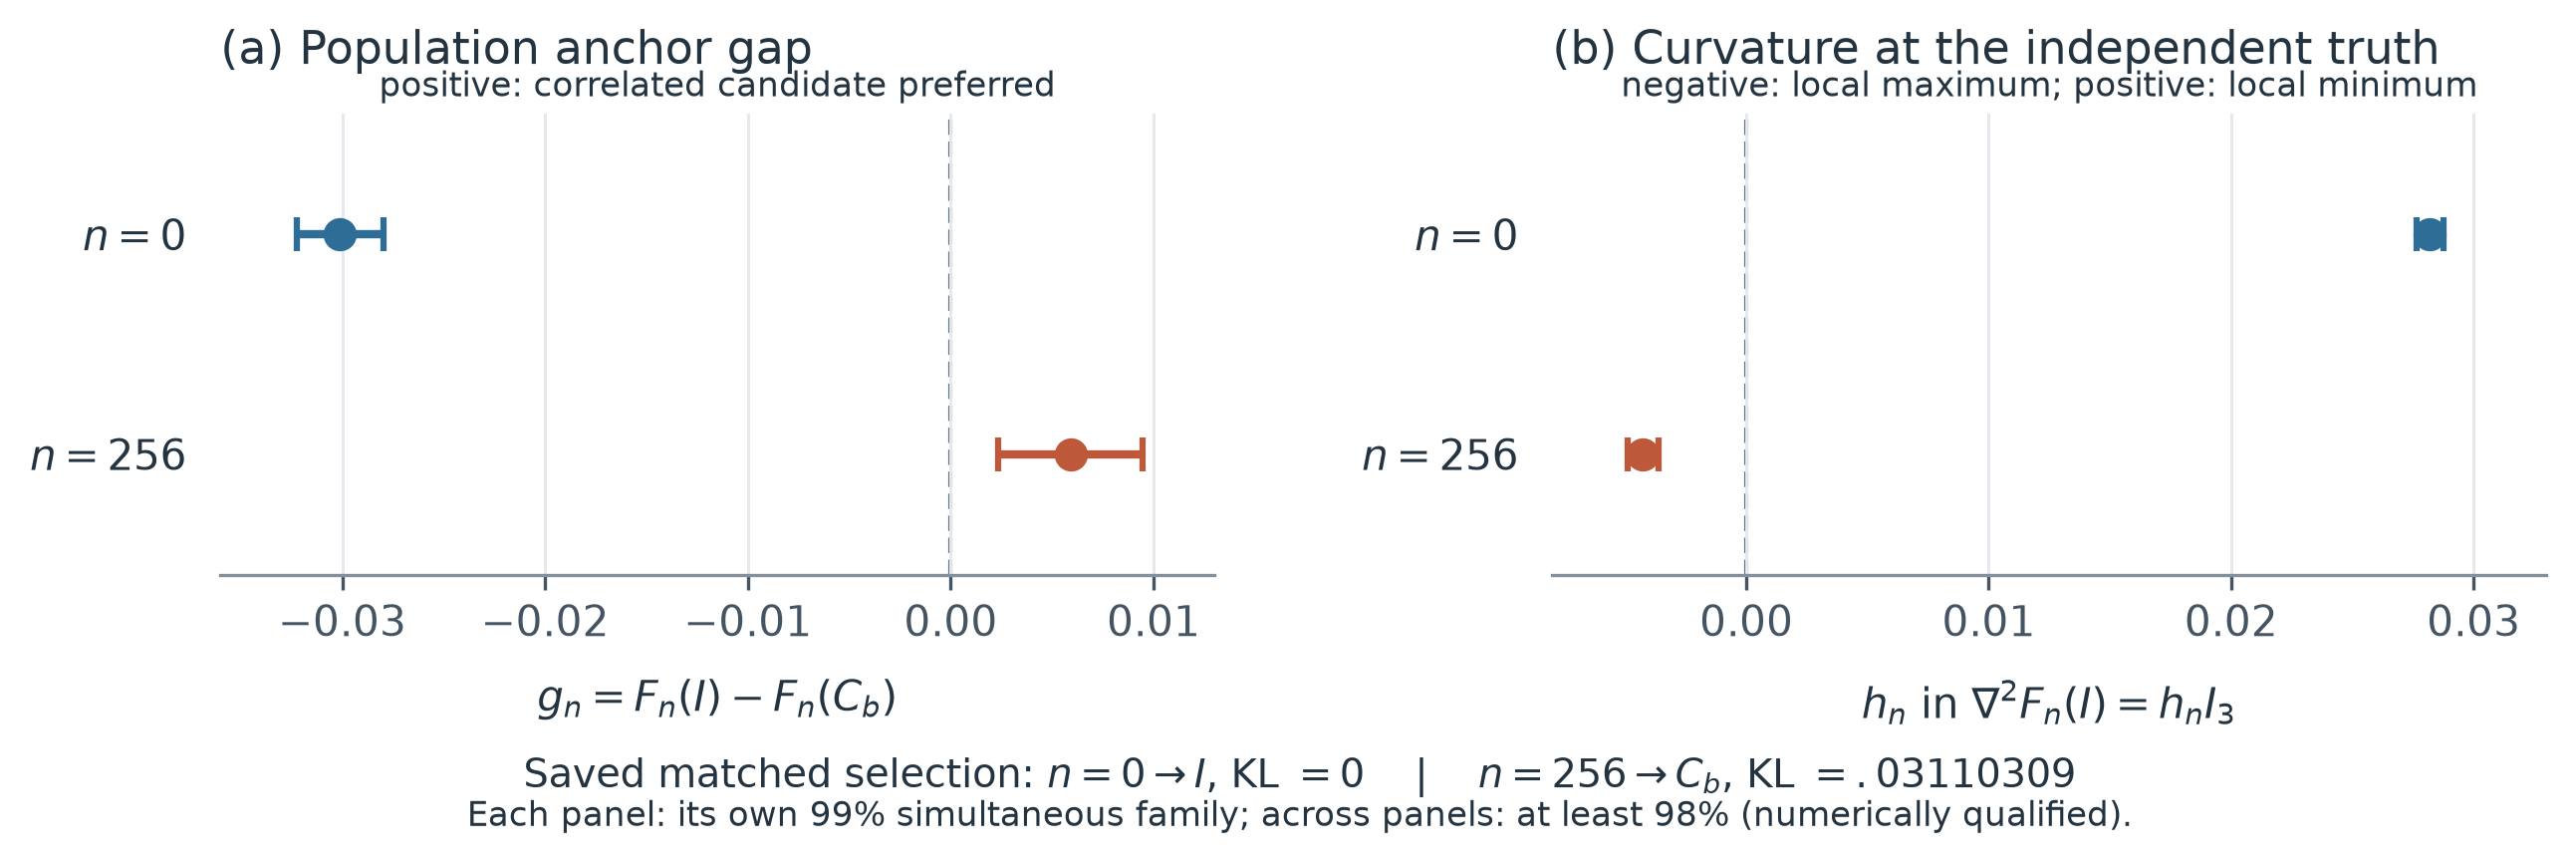
\includegraphics[width=1\linewidth,height=\textheight,keepaspectratio,alt={The fair-coin control. Three binary variables with independent latent logits (C\_*=I), K=100 particles per logarithm. (a) Population gap g\_n=F\_n(I)-F\_n(C\_b) between the truth and the equicorrelated candidate C\_b; positive values mean the finite objective prefers C\_b. (b) Curvature h\_n of the objective at the truth, where \textbackslash nabla\^{}2F\_n(I)=h\_nI\_3 in the three free correlations; negative values make the truth a local maximum. At n=256, the appended fair coins' per-particle likelihoods stay inside the particle average; active observations, active particles and candidates are shared with n=0. Bars are 99\% simultaneous intervals for each panel under ideal iid sampling and stated numerical allowances (Appendix C.2, C.4); positivity of h\_0 is also proved analytically (C.3). The footer reports one matched 143-point grid selection (C.1).}]{figures/finite_instance.png}
\caption{The fair-coin control. Three binary variables with independent
latent logits (\(C_*=I\)), \(K=100\) particles per logarithm. (a)
Population gap \(g_n=F_n(I)-F_n(C_b)\) between the truth and the
equicorrelated candidate \(C_b\); positive values mean the finite
objective prefers \(C_b\). (b) Curvature \(h_n\) of the objective at the
truth, where \(\nabla^2F_n(I)=h_nI_3\) in the three free correlations;
negative values make the truth a local maximum. At \(n=256\), the
appended fair coins' per-particle likelihoods stay inside the particle
average; active observations, active particles and candidates are shared
with \(n=0\). Bars are 99\% simultaneous intervals for each panel under
ideal iid sampling and stated numerical allowances (Appendix C.2, C.4);
positivity of \(h_0\) is also proved analytically (C.3). The footer
reports one matched 143-point grid selection (C.1).}
\end{figure*}

\textbf{A controlled comparison.} Take three binary observations whose
latent Gaussian logits are independent, and use \(K=100\) particles. Now
append \(n\) further observed binary variables that are fair coins
independent of everything else. Each coin has its own latent logit
\(G_j\sim N(0,1)\) and emission probability \(\sigma(u_jG_j)\) for
outcome \(u_j\in\{-1,1\}\). Averaged over the prior, every coin has
probability \(1/2\) under every candidate. Each candidate's integrated
model is therefore its old model times \(2^{-n}\), and every risk is
unchanged. Inside the particle average the coins act differently.
Particle \(k\) carries the factor \(\prod_j\sigma(u_jG_{kj})\), which
varies from particle to particle even though its prior mean is
\(2^{-n}\). These factors decide which particles dominate the average,
and hence how the active likelihoods compete. Integrating the coins out
\emph{before} averaging would instead contribute the common constant
\(2^{-n}\) and change nothing.

Figure 1 compares \(n=0\) with \(n=256\) on the same active
observations, active particles and candidates. Without coins, the finite
objective prefers the true independent model to an equicorrelated
candidate \(C_b\) with all correlations \(.9\), and the truth is a
strict local minimum. With 256 coins the preference reverses: \(C_b\)
scores better, the truth becomes a local maximum, and a matched grid
search returns \(C_b\), whose risk is \(.031\) nats.

We regard this construction as a control, not as a recommended practice.
The appended block is known to be independent, and its likelihood
factorizes exactly. Its value is that it changes the estimator while
preserving the active likelihood ratios and every candidate's KL risk.
Whatever changes in Figure 1 is therefore the criterion's own
preference.

\textbf{Why a fine scale is needed.} As \(n\) grows, nuisance
log-weights spread on a scale \(\sqrt n\), and the average is dominated
by the particle with the largest nuisance weight. With fixed active
marginals, the expected loss of one prior particle is the same for every
candidate correlation matrix, so the leading term of the objective does
not see dependence at all. Heuristically, the leading selection term in
this regime comes from events where the two leading particles are nearly
tied, and such events have frequency of order
\(w_{n,K}\asymp\sqrt{\log K/n}\). Selection therefore happens at a scale
that shrinks with \(n\), and this has two consequences. An approximation
that gets the objective right to \(o(1)\) can be silent about which
correlations are chosen; it must be accurate relative to \(w_{n,K}\).
And identifying the preference requires controlling near-ties for the
actual, non-Gaussian log-likelihood weights, uniformly over candidates.
A Gaussian model of the log-weights formally predicts the large-\(K\)
coefficient but does not supply this control (Section 6).

Theorem 1 supplies it. The resulting potential is strictly concave and
has a direct reading: it rewards correlation matrices under which the
active log-likelihood of an observation varies more across prior draws.
For two variables with true correlation zero, the exact likelihood pulls
a fitted correlation back toward zero, while the limiting particle
objective pushes it away. Theorem 2 combines concavity with the
classical geometry of correlation matrices. Near-minimizers that resolve
the scale \(w_{n,K}\) are driven to the spectral boundary of the class
and keep their risk bounded away from zero.

\textbf{Without an appended block.} The coins make the mechanism
visible, but they leave a natural question. Suppose there is no
designated independent block, every bias and loading is learnable, and a
local minimum of the finite objective already reproduces every
observation marginal. Does the objective then at least not oppose
dependence changes that would lower the risk? Theorem 3 answers no for a
specific eight-item, two-factor model with \(K=8\). A computer-assisted
proof certifies a rank-one strict local minimum of the exact population
objective in all 24 parameters, modulo common rotations. All marginals
are correct and the joint KL is about \(.0104\). Along a path that
rotates loading rows without changing their lengths, every sufficiently
small nonzero step lowers the risk and raises the objective. The two
parts thus answer successive questions about one criterion: an
asymptotic statement about \emph{selection} in a controlled family, then
a finite, \emph{local} statement about geometry without that control.
Neither is derived from the other.

\textbf{Contributions.}

\begin{itemize}
\tightlist
\item
  A uniform selection-scale theorem for the actual non-Gaussian weights,
  covering every fixed \(K\ge2\) and \(K\) growing polynomially in
  \(n\), together with a conditional-variance reading of the limiting
  potential (Theorem 1).
\item
  Its geometric consequence: a spectral-boundary preference and positive
  limiting risk for population near-minimizers with regret
  \(o(w_{n,K})\) (Theorem 2).
\item
  A finite-scale analysis: a signed fixed-\(K\) correction isolates the
  same-particle coupling that scalar overlap misses, and explicit bounds
  certify the leading sign of one coordinate at \(n=4096\) (Section 4).
\item
  A computer-assisted certificate of a marginal-correct, risk-positive
  local minimum with a same-root, marginal-preserving conflict,
  persisting over a small explicit teacher family (Theorem 3 and its
  corollary).
\end{itemize}

The main theory concerns population objectives with particles drawn from
the prior; Section 4.3 adds guarantees for one specified finite program.
None describes where a stochastic optimizer converges.

\section{Prior-Particle Objectives and a Controlled
Augmentation}\label{prior-particle-objectives-and-a-controlled-augmentation}

For latent \(Z\sim p(z)\) and conditional likelihood
\(p_\theta(y\mid z)\), the \(K\)-particle objective is
\(E_{Y\sim P}E_{Z_{1:K}}[-\log K^{-1}\sum_kp_\theta(Y\mid Z_k)]\), with
iid prior particles independent of \(Y\). At \(K=\infty\) it becomes the
integrated cross entropy. Our first model makes the active correlations
the only unknowns. Fix \(m\ge2\), a finite mean \(\mu\) and
\(0<\delta<1\):

\[
\begin{aligned}
\mathcal E_\delta^{(m)}
&=\{C=C^\top:\operatorname{diag}C=\mathbf1,\ C\succeq\delta I\},\\
X_A&=\mu+L_CZ,\qquad L_CL_C^\top=C,\\
X_{m+j}&=\tau_jG_j,\\
P(Y_i=y_i\mid X_i)&=\sigma(y_iX_i),\qquad y_i\in\{-1,1\}.
\end{aligned}
\tag{1}
\]

All Gaussian inputs are independent standard normals before applying
\(L_C\), and observations are conditionally independent given their
logits. Active variances and the mean are known, and active and nuisance
logits are uncorrelated. We write \(U\) for the nuisance observations
and assume the teacher \(C_*\) lies in the relative interior,
\(C_*\succ\delta I\). Because each nuisance coin is fair after
integration,

\[
Q_{C,\tau}^{(n)}(y,u)=2^{-n}Q_C^A(y),\qquad
\mathcal R(C)=D(Q_{C_*}^A\Vert Q_C^A).
\tag{2}
\]

This is also the KL risk of the complete observation. Changing nuisance
scales at fixed \(n\) leaves the whole observation law unchanged;
changing \(n\) leaves active likelihood ratios and the KL unchanged.
With \(K\) iid prior particles \((Z_k,G_k)\) independent of the
observation,

\[
\begin{aligned}
\widehat Q_{C,\tau,K}^{(n)}(y,u)
&=K^{-1}\sum_{k=1}^Kp_{C,\tau}(y,u\mid Z_k,G_k),\\
F_{n,K}(C;\tau)&=E_{Y,U,Z,G}[-\log\widehat Q_{C,\tau,K}^{(n)}(Y,U)].
\end{aligned}
\tag{3}
\]

Each realized mixture \(\widehat Q\) is a normalized distribution, so
\(F-H(P)=E_{Z,G}D(P\Vert\widehat Q)\). The finite objective scores a
random mixture, while the risk scores its average. Suppressing fixed
arguments, the gap between the two is the classical Jensen term:

\[
\begin{aligned}
F_P(C)&=H(P)+\mathcal R(C)+\mathcal J_P(C),\\
\mathcal J_P(C)&=E_P[\log Q_C\\
&\qquad -E_{Z,G}\log\widehat Q_C]\ge0.
\end{aligned}
\tag{4}
\]

Here \(P=Q_{C_*}^{(n)}\). Nonnegativity of \(\mathcal J_P\) is standard;
what matters for learning is how \(\mathcal J_P\) varies with \(C\),
which nonnegativity alone does not determine. This is consistent with
properness of the logarithmic score, because \(F\) is the expected score
of a random predictive rule rather than of \(Q_C\). Two further facts
fix what the augmentation does and does not do. Transporting the prior,
emissions and particles by an invertible latent map leaves every
realization of \(\widehat Q\) unchanged (Appendix A.1), whereas
appending observed coordinates changes the estimator. And at \(K=1\) the
objective depends only on the fixed marginals, so it is constant in
\(C\): any dependence selection requires \(K\ge2\).

\section{Which Correlations the Finite Objective
Prefers}\label{which-correlations-the-finite-objective-prefers}

\subsection{The Selection Scale}\label{the-selection-scale}

Write \(b_i=EY_i\) and \(\kappa_{ij}(c)\) for the covariance of
\(Y_i,Y_j\) when their latent correlation is \(c\). Fixed marginals make
\(b_i\) independent of \(C\), and Price's identity \citep{price1958}
gives

\[
\begin{aligned}
\kappa_{ij}(0)&=0,\\
\kappa_{ij}'(c)&=\tfrac14 E_C[\operatorname{sech}^2(X_i/2)\\
&\qquad\quad{}\times\operatorname{sech}^2(X_j/2)]>0.
\end{aligned}
\tag{5}
\]

So observed covariances identify latent correlations. Differentiating
the objective weights a per-particle \emph{dependence mark} by how much
that particle shares the average. With \(\pi_k\) the normalized
\textbf{complete} particle likelihoods, which include the nuisance
factors,

\[
\begin{aligned}
\partial_{c_{ij}}F_{n,K}
&=-E\sum_k\pi_k(1-\pi_k)H_{k,ij},\\
H_{k,ij}&=Y_iY_j\sigma(-Y_iX_{ki})\sigma(-Y_jX_{kj}),\\
EH_{k,ij}&=\{\kappa_{ij}(C_*)+\kappa_{ij}(C)\}/4.
\end{aligned}
\tag{6}
\]

The mean of the mark follows because labels and candidate particles are
independent. At finite \(n\), however, a particle's weight and its mark
are coupled, which will matter in Section 4.

Set nuisance scales to one, write \(F_{n,K}^*(C)=F_{n,K}(C;\mathbf1)\),
and define

\[
\begin{gathered}
v=\operatorname{Var}\log\sigma(G),\qquad J_K=E\max_{k\le K}G_k,\\
w_{n,K}=J_K/\sqrt{nv}.
\end{gathered}
\tag{7}
\]

Here \(J_K\) is the expected maximum of \(K\) standard Gaussians, with
\(J_K\sim\sqrt{2\log K}\) and \(J_K^2\asymp1+\log K\) for integers
\(K\ge2\) (Appendix A.2). Hence \(w_{n,K}\asymp\sqrt{\log K/n}\) in the
polynomial range below, and \(w_{n,K}\asymp n^{-1/2}\) at fixed \(K\). A
heuristic explains the scale. If the \(K\) nuisance log-weights were
Gaussian with standard deviation \(\sqrt{nv}\), the density at zero of
the gap between the largest two would be
\(K(K-1)\int\phi^2\Phi^{K-2}/\sqrt{nv}=w_{n,K}\). An active
log-likelihood difference of order one changes the dominant particle
only on such near-ties.

\subsection{The Limiting Potential}\label{the-limiting-potential}

\textbf{Theorem 1 (uniform direction and potential).} Fix
\(m,\mu,\delta\), \(C_*\in\operatorname{relint}\mathcal E_\delta^{(m)}\)
and \(C_0,p>0\). As \(n\to\infty\), uniformly over
\(C\in\mathcal E_\delta^{(m)}\) and integers \(2\le K\le C_0n^p\),

\[
\begin{aligned}
\frac{\partial_{c_{ij}}F_{n,K}^*(C)}{w_{n,K}}
&\longrightarrow-\frac{\kappa_{ij}(C_*)+\kappa_{ij}(C)}4,\\
\frac{F_{n,K}^*(C)-F_{n,K}^*(I)}{w_{n,K}}
&\longrightarrow V(C),\\
V(C)&=-\frac14\sum_{i<j}\Bigl[\kappa_{ij}(C_*)c_{ij}\\
&\qquad\qquad+\int_0^{c_{ij}}\kappa_{ij}(u)\,du\Bigr].
\end{aligned}
\tag{8}
\]

The proof (Appendix A.1--A.2) works with the actual log-sigmoid nuisance
weights. It controls nearly tied pairs of nuisance log-weights through
uniform moderate-tail and density estimates valid for polynomial \(K\),
together with a common envelope for active scores over the
fixed-dimensional correlation class. Compactness alone does not give
control at a shrinking scale. Integrating the gradient along the
feasible segment from \(I\) to \(C\) gives \(V\).

Three readings make (8) concrete.

\emph{The Jensen gap absorbs the risk.} Differences of \(F^*_{n,K}\)
vanish at rate \(w_{n,K}\), while risk differences
\(\mathcal R(C)-\mathcal R(I)\) do not depend on \(n\). By (4), the
\(C\)-dependence of the Jensen term therefore cancels the risk
differences to leading order. What survives at scale \(w_{n,K}\) is
\(V\), which can rank correlations differently from observation risk.

\emph{What \(V\) rewards.} Let \(A_C(y,Z)=\sum_i\log\sigma(y_iX_i)\) be
the active log-likelihood of label \(y\) at one prior draw, and
\(T(C)=E_Y\operatorname{Var}_ZA_C(Y,Z)\) its variance across prior
draws, averaged over true labels. Price's identity gives
\(\partial_{c_{ij}}T=\{\kappa_{ij}(C_*)+\kappa_{ij}(C)\}/2\), so

\[
V(C)=-\tfrac12\{T(C)-T(I)\}.
\]

The limiting objective prefers correlation matrices under which an
observation's active log-likelihood is more variable across prior draws.
This is the conditional variance of the active log-likelihood, not the
variance of the likelihood itself, of the nuisance weights, or of a
stochastic gradient (Appendix B.1).

\emph{Two variables.} With centred variables, true correlation
\(\theta\) and spin moment \(r(\rho)\), the exact cross entropy has
derivative \(r'(\rho)\{r(\rho)-r(\theta)\}/\{1-r(\rho)^2\}\). Its
descent moves \(\rho\) toward \(\theta\). At \(\theta=0\), the limiting
particle gradient \(-\kappa(\rho)/4\) has the opposite sign, so descent
moves a nonzero correlation away from zero. More generally, by (5) the
Hessian of \(V\) in correlation coordinates is diagonal with strictly
negative entries: \(V\) is strictly concave.

\subsection{Spectral Boundary and
Risk}\label{spectral-boundary-and-risk}

A strictly concave function on a compact convex set attains its minimum
only at extreme points. For correlation matrices, those points are
constrained by a classical rank bound \citep{litam1994}.

\textbf{Theorem 2 (spectral preference and risk).} Under Theorem 1, let
\(\mathcal M=\arg\min_{\mathcal E_\delta^{(m)}}V\) and
\(r_{\max}=\lfloor(\sqrt{8m+1}-1)/2\rfloor\). Every \(C\in\mathcal M\)
satisfies

\[
\operatorname{rank}\left(\frac{C-\delta I}{1-\delta}\right)\le r_{\max}.
\tag{9}
\]

At least \(m-r_{\max}\) eigenvalues therefore equal \(\delta\), while
\(C\) remains positive definite. For integer sequences
\(2\le K_n\le C_0n^p\) eventually, if
\(\widehat C_n\in\mathcal E_\delta^{(m)}\) has population regret
\(F_{n,K_n}^*(\widehat C_n)-\inf_C F_{n,K_n}^*(C)=o(w_{n,K_n})\), then

\[
\begin{gathered}
\operatorname{dist}(\widehat C_n,\mathcal M)\to0,\\
\liminf_n\mathcal R(\widehat C_n)
\ge\varepsilon_*,\\
\varepsilon_*:=\min_{C\in\mathcal M}\mathcal R(C)>0.
\end{gathered}
\tag{10}
\]

The constant depends on \((m,\mu,\delta,C_*)\). The affine map in (9)
sends \(\mathcal E_\delta^{(m)}\) to a set of correlation matrices,
where an extreme point of rank \(r\) satisfies \(r(r+1)/2\le m\). The
monotonicity in (5) identifies latent correlations from observed
moments, and compactness separates \(\mathcal M\) from the interior
teacher in observation KL (Appendix A.3). For example, in the
four-variable fixture (A.21), with \(\mu=(-.6,-.2,.2,.6)\),
\(\delta=.1\) and teacher eigenvalues \((.5,1,1.2,1.3)\), at least two
limiting eigenvalues equal \(.1\) and
\(\liminf_n\mathcal R(\widehat C_n)\ge9/12800\).

``Spectral boundary'' here means eigenvalues at the floor \(\delta\).
The selected matrix is positive definite, and individual correlations
need not all grow. For random outputs with \(o_p(w_{n,K_n})\) regret,
the distance to \(\mathcal M\) tends to zero in probability and
\(P\{\mathcal R(\widehat C_n)<\varepsilon_*-\eta\}\to0\) for every
\(\eta>0\). The theorem concerns population regret, not every finite
dataset: an empirical label distribution changes the linear term of
\(V\), and a one-label dataset can share its exact and particle
minimizers (Appendix A.6).

\textbf{Other parameter regimes.} Two variants show that the regime
matters. If active means and scales are also free, with means in a
compact box containing the logits of the true marginal probabilities,
scales in \([0,S]^m\) and the coins still at unit scale, then \(o(1)\)
population regret already drives the active scales to zero. The
observation law converges to the product of the true marginals, and the
risk tends to the teacher's total correlation (Appendix A.8). If instead
the common nuisance scale is learnable and may reach zero, joint
minimization switches the coins off: the extra nuisance penalty
disappears, leaving the active finite-\(K\) objective with its own bias
(Appendix A.9). Theorems 1--2 hold nuisance scales at one, which is
exactly what makes the coins a control.

\section{How the Asymptotic Picture Meets Finite
Scales}\label{how-the-asymptotic-picture-meets-finite-scales}

Theorem 1 gives no remainder bound at any finite \(n\). We therefore
examine one instance closely: \(m=3\), \(\mu=0\), \(C_*=I\),
\(\delta=.1\) and \(K=100\). Let \(C(\rho)\) have all off-diagonals
\(\rho\) and \(C_b=C(.9)\). At \(n=64,256,1024,4096\) we compare the gap
\(g_n=F_n(I)-F_n(C_b)\) and the free \(c_{12}\) derivative \(D_n\) at
\(C(.45)\) with their leading predictions, using \(F_n=F_{n,100}^*\) and
\(w_n=w_{n,100}\). The ratios \(A_n=g_n/\{w_n[V(I)-V(C_b)]\}\) and
\(B_n=-D_n/(m_H^{\mathrm{ref}}w_n)\) equal one when the leading term is
exact; \(m_H^{\mathrm{ref}}\) is a fixed numerical reference for
\(\kappa(.45)/4\).

\subsection{Weight Overlap Is Not the Learning
Signal}\label{weight-overlap-is-not-the-learning-signal}

A natural shortcut is to track scalar weight overlap
\(\omega_n=E\sum_k\pi_k(1-\pi_k)\), which measures how much of the
average is shared between particles. If marks were independent of
weights, (6) would give \(D_n=-m_H\omega_n\). At \(n=64\) overlap
matches its leading scale closely, \(\omega_n/w_n\simeq.992\). Yet
\(A_n\simeq-.143\) and \(B_n\simeq-.149\): both the gap and the
derivative have the \emph{opposite} sign to their leading predictions,
and the conditional intervals exclude zero. The identity
\(D_n=-m_H^{\mathrm{ref}}\omega_n-\mathcal C_n\), with
\(\mathcal C_n=E\sum_k\pi_k(1-\pi_k)(H_{k,12}-m_H^{\mathrm{ref}})\),
separates the overlap error \(O_n\) from weight--mark coupling \(J_n\)
(Figure 2b). Coupling dominates in magnitude at 64, 256 and 1024. By
4096 the point estimates of \(A_n\) and \(B_n\) are about \(.83\), but
the intervals do not certify 10\% relative accuracy. Complete weights
also contain active scores, so the split is an identity, not a causal
decomposition (Appendix C.6).

\begin{figure*}[t]
\centering
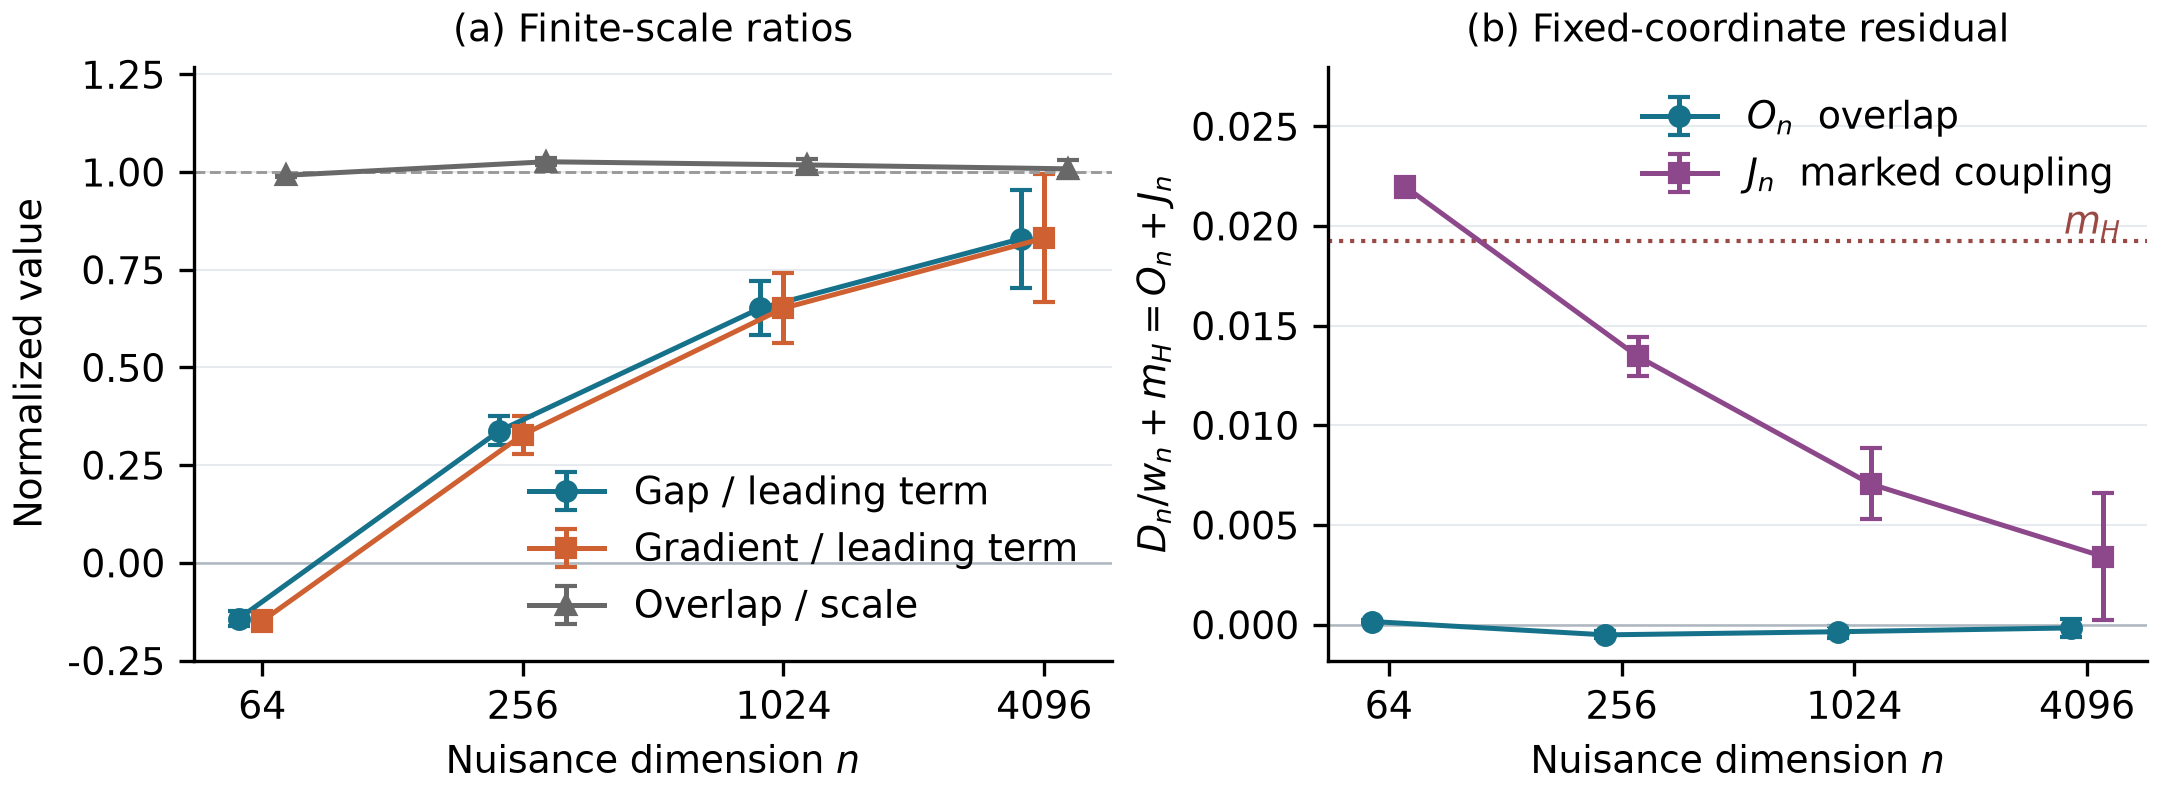
\includegraphics[width=1\linewidth,height=\textheight,keepaspectratio,alt={Finite scales with 100 particles; n counts appended fair coins. (a) Gap, free-coordinate gradient and scalar overlap relative to their leading predictions; negative ratios reverse the predicted sign. (b) Gradient residuals at C(.45), separated into overlap error O\_n and weight--mark coupling J\_n; the label m\_H denotes the fixed numerical reference m\_H\^{}\{\textbackslash mathrm\{ref\}\}. Bars are conditional 99\% simultaneous intervals for 26 targets under ideal iid sampling and stated numerical allowances; the 131,072 banks are shared across n, and the last paired increase in B\_n is unresolved (Appendix C.6).}]{figures/bridge_summary_en.png}
\caption{Finite scales with 100 particles; \(n\) counts appended fair
coins. (a) Gap, free-coordinate gradient and scalar overlap relative to
their leading predictions; negative ratios reverse the predicted sign.
(b) Gradient residuals at \(C(.45)\), separated into overlap error
\(O_n\) and weight--mark coupling \(J_n\); the label \(m_H\) denotes the
fixed numerical reference \(m_H^{\mathrm{ref}}\). Bars are conditional
99\% simultaneous intervals for 26 targets under ideal iid sampling and
stated numerical allowances; the 131,072 banks are shared across \(n\),
and the last paired increase in \(B_n\) is unresolved (Appendix C.6).}
\end{figure*}

\subsection{A Signed Correction and a Certified
Direction}\label{a-signed-correction-and-a-certified-direction}

What scalar overlap misses can be identified at fixed \(K\). Write
\(L=\log\sigma(G)\), \(\kappa_3=E(L-EL)^3\), \(s_n=\sqrt{nv}\) and
\(B_K=EM_K^2-1\), where \(M_K=\max_{k\le K}G_k\). For one candidate
particle, let \(A_Y=\sum_i\log\sigma(Y_iX_i)\), \(H_Y=H_{1,12}\) from
(6), \(m_H=EH_Y\) and \(\bar c=E_Y\operatorname{Cov}_X(H_Y,A_Y)\).

\protect\phantomsection\label{fixed-k-proposition}
\textbf{Proposition (fixed-K correction).} In the centred model (1) with
unit nuisance scales, fix \(m\), a positive definite candidate \(C\), a
teacher label law and an integer \(K\ge2\). Then, as \(n\to\infty\),

\[
\begin{aligned}
D_n:=\partial_{c_{12}}F_{n,K}^*(C)
&=-\frac{m_HJ_K}{s_n}\\
&\quad+\frac{B_K}{s_n^2}
 \left(\frac{m_H\kappa_3}{3v}-\bar c\right)\\
&\quad+O_{K,m,C}(n^{-3/2}).
\end{aligned}
\tag{11}
\]

The new ingredient is \(\bar c\): a covariance \emph{within one
particle}, between its dependence mark and its active log-likelihood,
computed given the label and then averaged over labels. It is not a
covariance between particles or between training gradients. Particles
with high active likelihood receive more weight; when their marks differ
systematically, the weighted mark is shifted. For the instance above at
\(C=C(.45)\), the \(n^{-1}\) coefficient is \(b_2\simeq1.026\). It
splits into a nuisance-skewness part \(\simeq-.077\) and a mark--score
part \(\simeq1.103\) (Appendix C.13). The correction thus opposes the
leading term and comes almost entirely from same-particle coupling.
These coefficients are model integrals rather than fits to the gradient
panel, although the panel was available when the correction was derived.
The proposition holds at fixed \(K\) and does not replace the uniform
statement of Theorem 1.

\protect\phantomsection\label{finite-direction-corollary}
\textbf{Finite-scale corollary.} At \(m=3\), \(\mu=0\), \(C_*=I\),
\(K=100\), \(C=C(.45)\) and the single free \(c_{12}\) coordinate,
explicit error bounds give

\[
\begin{gathered}
-.002045393<D_{4096}<-.0003519373,\\
|D_{4096}-D_{4096}^{(0)}|<.001097138798\\
<|D_{4096}^{(0)}|,\qquad
D_n^{(0)}=-m_HJ_{100}/s_n.
\end{gathered}
\tag{12}
\]

At \(n=4096\) the leading term has the correct sign for this coordinate.
The error bound is about 75.7\% of \(|D_{4096}^{(0)}|\), so the
certificate is about sign, not 10\% accuracy. At 64, 256 and 1024 the
same recipe leaves the sign unresolved. The enclosures are deterministic
and use the actual Gumbel-smoothed nuisance noise and certified model
moments (\hyperref[fixed-k-correction]{Appendix C.7 onward}).

The certified sign has a risk consequence. By (5) and the three-variable
law,
\(\partial_{c_{12}}\mathcal R=\kappa'(.45)\kappa/\{(1-\kappa)(1+3\kappa)\}>0\)
with \(\kappa=\kappa(.45)>0\). Every sufficiently small feasible
increase of \(c_{12}\) therefore lowers \(F^*_{4096,100}\) while raising
the risk. This is a finite, coordinate-level objective--risk conflict,
established by its own explicit remainder bounds rather than by Theorem
2.

\subsection{\texorpdfstring{Finite-Program Consequences at
\(n=256\)}{Finite-Program Consequences at n=256}}\label{finite-program-consequences-at-n256}

The instance of Figure 1 also yields finite-program statements at
\(n=256\), \(K=100\) (Appendix C.15, D, E). On a 99\% audit event under
ideal iid sampling and declared numerical conditions, every correlation
matrix in the class with population regret below \(.00134\), on or off
the grid, has risk above \(10^{-6}\); this excludes a continuous
low-risk region under a near-optimality condition that no algorithm is
shown to attain. On the same event, a fresh run of the fixed 143-point
grid program selects risk at least \(0.09/(32e)\) with probability at
least \(.7035\), a bound on a probability for that program rather than
an observed frequency.

\section{Without an Appended Block: A Certified Local
Conflict}\label{without-an-appended-block-a-certified-local-conflict}

\subsection{A Two-Factor Model with All Parameters
Free}\label{a-two-factor-model-with-all-parameters-free}

We now remove the control. There is no designated independent block; all
biases and loadings are learned:

\[
\begin{aligned}
Z&\sim N(0,I_2),\qquad \theta=(b,W),\\
Y_j\mid Z&\sim\operatorname{Bernoulli}
 \{\sigma(b_j+w_j^\top Z)\},\\
F_K^q(\theta)&=E_{Y\sim q,Z_{1:K}}\Bigl[
-\log\Bigl\{K^{-1}\sum_{k=1}^K
p_\theta(Y\mid Z_k)\Bigr\}\Bigr].
\end{aligned}
\tag{13}
\]

Here \(b\) collects logit biases, \(Y_j\in\{0,1\}\), and the prior
particles \(Z_{1:K}\) are iid and independent of \(Y\). Items are
conditionally independent given \(Z\). The target \(q\) is empirical or
the teacher law, and \(F_\infty^q\) is the integrated cross entropy. The
teacher has eight items, zero biases and rows of length \(.8\) at angles
\((-.7,-.5,-.3,-.1,.1,.3,.5,.7)\), so all pairwise loading inner
products are positive. This class differs from Section 3: the logit
covariance \(WW^\top\) has rank at most two and no spectral floor, and
loading rank is not the rank of \(\operatorname{Cov}(Y)\).

\subsection{Correct Marginals, Positive Risk, and an Opposed
Improvement}\label{correct-marginals-positive-risk-and-an-opposed-improvement}

\textbf{Theorem 3 (computer-assisted local dependence conflict).} For
the exact teacher in (13), let \(q_*\) be its observation law and
\(\mathcal R(\theta)=D(q_*\Vert Q_\theta)\). There is a rank-one
interior parameter \(\theta_*=(0,a_*,0)\), with \(a_{*,i}>0\) and
\(\nabla F_8^{q_*}(\theta_*)=0\), that is a strict local minimum of
\(F_8^{q_*}\) in the full 24-dimensional parameter space modulo common
latent rotations. Every observation marginal is correct,
\(Q_{\theta_*}(Y_j=1)=q_*(Y_j=1)=1/2\), yet
\(\mathcal R(\theta_*)\simeq.01043>0\).

There is a fixed
\(d=d_{\mathrm{ang}}^{(8)}\in\mathbf1^\perp\subset\mathbb R^8\),
\(\|d\|_2=1\), such that the path \(\theta_{\mathrm{ang}}(t)=(0,W(t))\)
satisfies

\[
\begin{aligned}
W_i(t)&=a_{*,i}\bigl(\cos(td_i),\sin(td_i)\bigr),\\
r(t)&=\mathcal R(\theta_{\mathrm{ang}}(t)),\\
r'(0)&=0,\qquad r''(0)<-.00450377.
\end{aligned}
\tag{14}
\]

There exists \(\varepsilon>0\) such that, for every
\(0<|t|<\varepsilon\),

\[
\begin{gathered}
F_8^{q_*}(\theta_{\mathrm{ang}}(t))>F_8^{q_*}(\theta_*),\\
\mathcal R(\theta_{\mathrm{ang}}(t))<\mathcal R(\theta_*),\\
\operatorname{rank}W(t)=2.
\end{gathered}
\tag{15}
\]

The path changes only dependence. Row lengths are fixed, so each
candidate logit keeps its Gaussian marginal \(N(0,a_{*,i}^2)\) and each
observation stays a fair coin, while
\(\operatorname{Cov}(X_i(t),X_j(t))=a_{*,i}a_{*,j}\cos\{t(d_i-d_j)\}\)
changes. These preserved logit variances are the candidate's own, not
the teacher's \(.8^2\). Since the root is a strict local minimum and a
nonconstant angle path leaves the rotation orbit, the objective rises
along it. The risk falls because its curvature along the path is
negative. The conflict is second order and local: every sufficiently
small nonzero step along this path lowers risk and raises the objective
(Appendix I.10). Fixed row lengths define this comparison path; they are
not a constraint on the learning problem. The full statement in
\hyperref[full-local-statement]{Appendix I.8} also certifies a direction
\(d_{\mathrm{risk}}\) with a negative first-order risk derivative; a
certified step of size \(10^{-7}\) along it raises \(F_8\), lowers the
risk and keeps the observation marginals fair, while changing row
lengths.

For scale, in four training streams of \(4096\) teacher samples,
independent-Bernoulli fits have KL about \(.107\) and Adam training with
\(K=8\) ended near \(.011\) (Appendix I.4); a refitted stationary point
of the integrated objective within the collinear submodel has KL about
\(.0070\) (I.6). These are numerical comparisons, not certified optima.

\textbf{Certificate outline.} Symmetry reduces root finding to four
coordinates, and interval root inclusion proves an exact stationary
point near a dyadic centre. Full-space stability needs every direction.
All 16 bias/radial and seven non-rotation transverse directions have
certified positive curvature; an angular check alone would not suffice
(\hyperref[full-hessian-criterion]{Appendix I.2},
\hyperref[full-local-statement]{I.8}). The risk curvature along (14)
includes the path acceleration. It is enclosed over all 256 labels by
Gaussian integration by parts, analytic quadrature error bounds
\citep{trefethen2014} and midpoint-radius arithmetic
\citep{johansson2017}, then transferred from the centre to the root by a
Lipschitz bound in the row lengths (\hyperref[same-root-angle]{I.10}).

\protect\phantomsection\label{quantitative-persistence-corollary}
\textbf{Corollary (quantitative local persistence).} Keep all eight
teacher biases zero and row lengths \(4/5\), changing only its first
angle to \(-.7+\lambda\), \(|\lambda|\le.001\). With observation law
\(q_\lambda\), there is a smooth branch
\(\theta_\lambda=(0,a(\lambda),0)\) connected to Theorem 3's root, each
a full-space strict local minimum of its own \(F_8^{q_\lambda}\) modulo
rotation. Using the same fixed \(d\) and replacing \(a_*\) by
\(a(\lambda)\) in (14) gives, for each teacher and every sufficiently
small nonzero \(|t|<\varepsilon_\lambda\), a rank-two path that raises
its finite objective and lowers its own risk
\(D(q_\lambda\Vert Q_\theta)\), preserving candidate Gaussian logit
marginals and correct fair observation marginals.

This teacher family breaks the symmetry of the original teacher, but it
is small: endpoint observation laws differ by about \(1.6\times10^{-4}\)
in \(L^1\) (\hyperref[teacher-family-full-statement]{Appendix I.11}).
For broader, unquantified perturbations of the teacher,
\hyperref[local-persistence]{Appendix I.9} shows that a nearby rank-one
strict local minimum survives with a first-order risk-decreasing
direction.

\subsection{Weak-Loading Intuition for
Alignment}\label{weak-loading-intuition-for-alignment}

A weak-loading expansion at fixed \(K>2\) gives intuition, though not a
quantitative account (Appendix I.1). With row lengths fixed and loadings
of order \(\varepsilon\), the finite objective is, up to
angle-independent terms,
\(\varepsilon^4a_K\|c-\{K/(K-2)\}c_*\|^2+O(\varepsilon^6)\), where
\(a_K>0\) is given in (I.2) and \(c\) collects pairwise row inner
products after removing the common scale \(\varepsilon\). It rewards
inner products \emph{amplified} relative to the teacher's. With fixed
lengths, rows can amplify their inner products only by aligning. In the
independent-teacher case of Section 3, the limiting potential likewise
favours dependence that the teacher lacks. The two expansions are
derived separately, and neither explains the other. The weak-loading
stability boundary of the collinear configuration, \(K\simeq4.33\), does
not predict behaviour at loading \(.8\).

Numerical learning is consistent with this picture without establishing
it (Appendix I.4--I.7). In four streams, \(K=8\) training produced
nearly collinear loadings, whereas \(K=64\) and the integrated reference
did not. Refitted at each \(K\), the collinear point numerically changes
local type between \(K=11\) and \(12\); angle probes there change the
risk by only about \(.02\%\), an effect size that belongs to those
probes, not to the certified \(K=8\) conflict.

\section{Related Work}\label{related-work}

\textbf{Monte Carlo objectives and simulated likelihood.} The logarithm
of an unbiased likelihood estimator is biased, and the bias depends on
the parameters. This is established for simulated maximum likelihood in
discrete-choice models \citep{lee1995}, for Monte Carlo likelihood
inference, where increasing simulation accuracy inside the logarithm and
averaging a fixed-\(K\) log objective are distinct limits
\citep{sung2007}, and for Monte Carlo variational objectives
\citep{maddison2017}. For a nonnegative unbiased normalizing-constant
estimator, AESMC's Claim 1 writes the expected-log gap as a KL
divergence on an extended sampling space \citep{le2018aesmc}; that
divergence is not the observation risk of the integrated model studied
here. For dependence specifically, the abstract of \citet{geweke1997}
reports downward bias of serial-correlation estimates in GHK
simulated-likelihood experiments; we treat this as an empirical
precedent, not as something our mechanism explains.

\textbf{Weight degeneracy and gradient asymptotics.} High-dimensional
importance sampling \citep{agapiou2017, chatterjee2018}, particle-filter
collapse \citep{bengtsson2008, bickel2008, snyder2008} and multi-sample
gradient estimators \citep{rainforth2018, tucker2019} are well studied.
The large-\(K\) scale \(w_{n,K}\) matches the expected maximum-weight
excess in \citet{bickel2008}; dependence selection requires control at
that scale. The nearest result to Theorem 1 is \citet{daudel2026}
(Section D.4.1, equation (208)). Under a Gaussian random-field condition
on the log-weights, and with derivative--expectation interchange, the
subleading mean gradient follows the derivative of the log-weight
standard deviation. Through the conditional-variance identity of Section
3, that formula formally predicts our large-\(K\) coefficient. Its proof
uses independence between the standardized log-weight field and its
parameter derivative, which approximate Gaussianity does not preserve
(their Section 3.4). \citet{daudel2023} (Theorem 6) treats non-Gaussian
iid log-weight sums and gives scalar objective asymptotics; that scalar
remainder cannot simply be differentiated into a correlation field that
is uniform at the smaller selection scale. What Theorem 1 adds is this
control for the actual non-Gaussian weights, uniform over the
correlation class and over \(2\le K\le C_0n^p\), including every fixed
\(K\ge2\). Theorem 2 then combines it with the classical extreme-point
geometry of correlation matrices \citep{litam1994} to reach an
observation-risk conclusion. Appendix B gives a theorem-level
comparison.

\textbf{Latent-variable learning and local geometry.} Learning binary
latent models by prior-sampled likelihood predates this work
\citep{tipping1998}. Importance-weighted autoencoders change their
learned representations when the objective changes \citep[Section 5.2
and Table 2]{burda2016}; our criterion is the negative of their bound
with the proposal fixed to the prior. A learned-proposal version is used
for item factor analysis \citep{urban2021}. Collapse and local stability
have been analysed in linear latent-variable models
\citep{lucas2019, wangziyin2022}; for linear VAEs, \citet{lucas2019}
(Theorem 1) rule out additional ELBO local maxima relative to the
marginal likelihood, and fixing the observation variance affects pPCA
stability. Theorem 3 instead certifies, in a nonlinear model, a
full-space local minimum of a finite-particle objective with a
marginal-preserving direction along which it opposes a risk improvement;
it is not a claim about low rank in general.

\section{Discussion}\label{discussion}

\textbf{What the results change.} At fixed \(K\) the prior-particle
objective has its own dependence preferences, and estimating it more
accurately does not move them toward the integrated likelihood. In the
controlled family these preferences are of order \(w_{n,K}\), yet they
decide which correlations are selected and yield positive limiting risk
(Theorems 1--2). In the finite-scale example, scalar overlap can track
its leading prediction while the correlation gradient has the opposite
sign to its own (Section 4). Correct marginals at a full-space local
minimum do not mean that the objective welcomes risk-reducing dependence
changes (Theorem 3).

\textbf{Scope.} The results carry different kinds of guarantee: Theorems
1--2 are uniform asymptotic statements; the corollary in (12) is a
deterministic enclosure at one \(n\); Section 4.3 rests on a 99\% audit
event with declared numerical conditions; Theorem 3 is a
computer-assisted local proof. All use prior particles, and apart from
the grid-program bound of Section 4.3 they concern population
objectives. The first part requires a known independent appended block
with unit scales, fixed active dimension and marginals, and regret small
relative to \(w_{n,K}\). The second part is one model with a small
explicit teacher family. A natural next question is whether learned,
posterior-adapted proposals \citep{burda2016} remove, shrink or reverse
this preference.

\textbf{Reproducibility.} The accompanying anonymous supplement provides
saved interval inputs, arithmetic checks for the certificates and
finite-program bounds, and data and scripts for Figures 1--2. Its README
gives the commands and verification scope. These checks reconstruct
saved evidence; they do not rerun production quadrature or training.
\FloatBarrier
\label{candidateMainEnd}
\section*{Impact Statement}\label{impact-statement}

This work aims to improve understanding of simulation-based
probabilistic learning. Its potential benefit is more reliable
separation of a random training criterion from the risk of the
integrated model. The studies use controlled synthetic observations,
without establishing deployment benefits. Applying the results requires
retaining their assumptions and finite-budget limitations, including the
reported recovery boundaries and negative controls.
\bibliographystyle{icml2026}
\bibliography{references}
\clearpage
\onecolumn
\setcounter{secnumdepth}{0}
\setcounter{figure}{0}
\renewcommand{\thefigure}{S\arabic{figure}}
\section*{Appendix reading guide}\label{appendix-reading-guide}

The retained appendices supply the proofs and evidence for the main-text
results. The table maps each main-text item to its support, with
continuous appendix lettering.

\begin{longtable}[]{@{}
  >{\raggedright\arraybackslash}p{(\linewidth - 4\tabcolsep) * \real{0.3333}}
  >{\raggedright\arraybackslash}p{(\linewidth - 4\tabcolsep) * \real{0.3333}}
  >{\raggedright\arraybackslash}p{(\linewidth - 4\tabcolsep) * \real{0.3333}}@{}}
\toprule\noalign{}
\begin{minipage}[b]{\linewidth}\raggedright
Main text
\end{minipage} & \begin{minipage}[b]{\linewidth}\raggedright
Where it is established
\end{minipage} & \begin{minipage}[b]{\linewidth}\raggedright
Type of support
\end{minipage} \\
\midrule\noalign{}
\endhead
\bottomrule\noalign{}
\endlastfoot
Figure 1, fair-coin control (Section 1) & C.1 matched selection; C.2 gap
audit; C.3 analytic curvature at \(n=0\); C.4 curvature audit at
\(n=256\) & Analytic bound at \(n=0\); 99\% audit families with stated
numerical allowances; one saved matched run \\
Model, decomposition and representation facts (Section 2) & A.1 &
Analytic \\
Selection scale, Theorem 1 (Section 3.1--3.2) & A.2; scale heuristic and
its relation to particle-filter collapse in B.2 & Uniform asymptotic
proof \\
Conditional-variance reading of \(V\) & B.1 & Exact identity \\
Theorem 2 and the four-variable example & A.3 (A.21--A.22) & Analytic \\
Other parameter regimes & A.8 (free active scales), A.9 (free nuisance
scale); further boundaries in A.4--A.7 & Analytic \\
Figure 2, overlap versus coupling (Section 4.1) & C.5--C.6 & Conditional
99\% simultaneous intervals, 26 targets \\
\hyperref[fixed-k-proposition]{Fixed-\(K\) correction} and
\hyperref[finite-direction-corollary]{finite-scale corollary} (Section
4.2) & \hyperref[fixed-k-correction]{C.7 onward}: proof C.8, budgets
C.9--C.12, constants and synthesis C.13, risk derivative C.14 &
Asymptotic proof; deterministic enclosure at \(n=4096\) \\
Finite-program consequences (Section 4.3) &
\hyperref[finite-evidence-summary]{C.15}; D (fresh-run bound); E
(saved-input arithmetic) & 99\% audit event, ideal iid sampling,
declared numerical conditions \\
Model (13) and weak-loading heuristic (Sections 5.1, 5.3) &
\hyperref[dense-model]{I.1} & Expansion with qualitative remainder \\
Theorem 3 (Section 5.2) & \hyperref[full-hessian-criterion]{I.2}
criterion (\hyperref[full-derivatives]{full derivatives});
\hyperref[laplace-representation]{I.3} representation;
\hyperref[proof-theorem-3]{I.8} root and
\hyperref[full-local-statement]{full-space statement};
\hyperref[same-root-angle]{I.10} same-root angular path &
Computer-assisted proof \\
\hyperref[quantitative-persistence-corollary]{Quantitative persistence
corollary} (Section 5.2) & \hyperref[quantitative-teacher-family]{I.11}
and \hyperref[teacher-family-full-statement]{full family statement} &
Computer-assisted proof over \(\lvert\lambda\rvert\le.001\) \\
Qualitative persistence (Section 5.2) &
\hyperref[local-persistence]{I.9} & Implicit-function argument;
neighbourhood not quantified \\
Numerical learning and K11/K12 probes (Section 5.3) & I.4--I.7 &
Numerical, with stated quadrature qualifications \\
\end{longtable}

\textbf{Material reported only in the appendices.} Known-mean robustness
and observation-equivalent scales (F); a two-particle counterexample
showing that matched means need not preserve finite-particle
stationarity (G); and the earlier finite selection and its negative
control (Appendix H).

A.2 retains the full uniform proof. Saved-endpoint and
certificate-composition checks do not recompute probability, gradient or
Hessian grids.

\clearpage

\section*{Appendix A. Proofs and representation
boundaries}\label{appendix-a.-proofs-and-representation-boundaries}

Theorem 1 is proved in A.1--A.2 and Theorem 2 in A.3. Here the star on F
denotes the fixed teacher: the appendix notation F with star and
nuisance scales is the same population score as in the main text. The
constant \(\varepsilon_*\) in Theorem 2 is the minimum risk on the
potential minimizing set; \(R_*\) in (A.19) is an explicit lower bound
for it. A.4--A.9 give the additional representation and scale
boundaries.

All logarithms are natural. Risk is the KL divergence for a complete
observation, without division by dimension. Throughout A.1--A.6, the
active dimension \(m\ge2\), mean vector \(\mu\in\mathbb R^m\), and
spectral floor \(0<\delta<1\) are fixed. Spin labels are
\(Y_i\in\{-1,1\}\); native API bits are \(Y_i^{(01)}=(Y_i+1)/2\).
Particle samples are independent of the observation being scored. The
population statements below do not assume that a finite optimization run
attains their required regret.

\subsection*{A.1. Model, exact task and the finite-particle
derivative}\label{a.1.-model-exact-task-and-the-finite-particle-derivative}

Learn the upper-triangular entries \(c_{ij}\), \(i<j\), of

\[
\begin{gathered}
\mathcal E_\delta^{(m)}
=\{C=C^\top:\operatorname{diag}C=\mathbf1,\ C\succeq\delta I\},\\
|c_{ij}|\le1-\delta,\qquad
\delta\le\lambda_{\min}(C)\le\lambda_{\max}(C)\le m-(m-1)\delta .
\end{gathered}
\tag{A.1}
\]

This is a compact convex set with nonempty relative interior in the
affine space of unit-diagonal symmetric matrices. Let
\(X\sim N(\mu,C)\), with conditionally independent emissions
\(P(Y_i=y_i\mid X_i)=\sigma(y_iX_i)\). Independent nuisance logits are
\(\tau_jG_j\), \(G_j\sim N(0,1)\), with the same logistic emission.
Symmetry gives

\[
\begin{aligned}
Q_C^A(y)&=E_C\prod_{i=1}^m\sigma(y_iX_i),&
Q_{C,\tau}^{(n)}(y,u)&=2^{-n}Q_C^A(y),\\
\widehat Q_{C,\tau,K}^{(n)}(y,u)
&=\frac1K\sum_{k=1}^K
\prod_{i=1}^m\sigma(y_iX_{ki})\prod_{j=1}^n\sigma(u_j\tau_jG_{kj}),\\
F_{n,K}^{*,\tau}(C)&=E_{(Y,U)\sim Q_{C_*}^{(n)},\,Z}
[-\log\widehat Q_{C,\tau,K}^{(n)}(Y,U)],&
\mathcal R_*(C)&=D(Q_{C_*}^A\Vert Q_C^A).
\end{aligned}
\tag{A.2}
\]

The true and candidate means and marginal variances agree. At a fixed
\(n\), changing nuisance scales preserves the whole observation law.
Across different \(n\), sample spaces differ; active likelihood ratios
and complete joint KL remain unchanged. Each realized particle predictor
is normalized, and its expectation is \(Q_C\); its expected log score
nevertheless differs from the log score of the integrated model.

This is distinct from a pure latent-coordinate change. For an invertible
measurable \(T_C\), push the prior forward, transport the emission by
\(p'_C(y\mid z')=p_C(y\mid T_C^{-1}z')\), and pair the particles. For
every realization and \(C\),

\[
\frac1K\sum_kp'_C(y\mid T_C(Z_k))
=\frac1K\sum_kp_C(y\mid Z_k).
\tag{A.3}
\]

Differentiable versions preserve path derivatives with respect to the
same physical \(C\) when all transport derivatives are included.
Changing optimization coordinates still requires the chain rule and need
not preserve Adam updates. Without paired samples, the estimator laws
agree rather than their realizations. Changing Gaussian nuisance scales
while retaining the uncompensated logistic emission is an
observation-equivalent representation change, not (A.3).

Write \(b_i=E Y_i=E\tanh((\mu_i+G)/2)\) and
\(\kappa_{ij}(c)=E_CY_iY_j-b_ib_j\). Fixed marginal means and variances
make this a function only of the pair correlation \(c\). Gaussian
integration by parts gives

\[
\kappa_{ij}(0)=0,\qquad
\kappa_{ij}'(c)=\frac14E_c[
\operatorname{sech}^2(X_i/2)\operatorname{sech}^2(X_j/2)]>0 .
\tag{A.4}
\]

\Needspace{10\baselineskip}

For one complete bank, let \(\pi_k\) be normalized complete particle
likelihoods and \(\gamma_k=\pi_k(1-\pi_k)\). Its mixed logit Hessian and
the off-diagonal Gaussian Price identity imply

\[
\begin{aligned}
\partial_{c_{ij}}F_{n,K}^{*,\tau}(C)
&=-E\sum_k\gamma_kH_{k,ij},\\
H_{k,ij}
&=Y_iY_j\sigma(-Y_iX_{ki})\sigma(-Y_jX_{kj})\\
&=(Y_i^{(01)}-\sigma(X_{ki}))(Y_j^{(01)}-\sigma(X_{kj})),\\
EH_{k,ij}&=\frac{\kappa_{*,ij}+\kappa_{ij}(c_{ij})}{4},
\qquad \kappa_{*,ij}=\kappa_{ij}(c_{*,ij}).
\end{aligned}
\tag{A.5}
\]

Indeed the mixed derivative for particle \(k\) is \(-\gamma_kH_{k,ij}\);
varying both symmetric covariance entries cancels the factor \(1/2\) in
Price's formula. Gaussian linear envelopes make the loss integrable and
justify differentiation; the mixed derivatives are bounded. Expanding
\(H\) as \([Y_iY_j-Y_iT_j-Y_jT_i+T_iT_j]/4\), \(T_i=\tanh(X_{ki}/2)\),
and using observation--particle independence proves its mean. A Price
sample is not generally equal to a realized Cholesky path derivative.

\subsection*{A.2. Uniform near-tie analysis and the matrix
potential}\label{a.2.-uniform-near-tie-analysis-and-the-matrix-potential}

We prove the direction result slightly more generally for prescribed
nuisance arrays \(a_{nj}\in[a_-,a_+]\), where \(0<a_-\le a_+<\infty\)
are fixed. The theorem's unit scales are included. Define

\[
\begin{gathered}
L_a=\log\sigma(aG),\quad v(a)=\operatorname{Var}L_a,\quad
s_n^2=\sum_{j=1}^nv(a_{nj}),\\
I_K=\int_{\mathbb R}\varphi(z)^2\Phi(z)^{K-2}\,dz,\qquad
J_K=K(K-1)I_K=E\max_{k\le K}G_k,\qquad w_{n,K}=J_K/s_n .
\end{gathered}
\tag{A.6}
\]

Since \(L_a=aG/2-\log2-\log\cosh(aG/2)\), odd/even orthogonality gives
\(v(a)\ge a^2/4\), while a Gaussian envelope gives \(s_n^2\asymp n\)
uniformly. Integration by parts proves the identity for \(J_K\). The
real-exponent argument below supplies \(J_K\sim\sqrt{2\log K}\) and
\(J_K^2\asymp1+\log K\) for integer \(K\ge2\).

The following steps keep the constants uniform. In the density estimates
they may depend on fixed \(a_-,a_+\) and the displayed truncation
levels, but not on \(n\), the nuisance array or its ordering. In the
pair estimate they may additionally depend on fixed \(C_0,p,C_1\). Only
the active-score envelope will introduce dependence on fixed
\(m,\mu,\delta\). Each \(o(1)\) has this uniform meaning. No explicit
convergence modulus for (A.13) is asserted.

\subsubsection*{Step 1. Uniform tilted densities: low and high
frequencies}\label{step-1.-uniform-tilted-densities-low-and-high-frequencies}

The density of \(L_a\), extended by zero for \(x\ge0\), is

\[
f_a(x)=\frac{\varphi(z_a(x))}{a(1-e^x)},\qquad
z_a(x)=\frac{x-\log(1-e^x)}a,\qquad x<0 .
\tag{A.7}
\]

These densities and each fixed-order derivative have uniform rapidly
decreasing envelopes for \(a\in[a_-,a_+]\). The left tail is Gaussian up
to polynomial factors. Near zero set \(t=-\log(-x)\); each fixed number
of derivatives contributes at most \(e^{ct}\) times a polynomial,
dominated by \(\exp[-t^2/(2a_+^2)+O(t)]\). The zero extension is
therefore smooth. The same bounds hold after an exponential tilt in a
sufficiently small fixed interval.

Let \(k_a(\lambda)=\log E e^{\lambda(L_a-EL_a)}\). Its fixed-order
derivatives are uniformly bounded for \(|\lambda|\le\lambda_0<1/4\); the
tilted variances are bounded away from zero by continuity and
nondegeneracy on this compact interval. For the centered tilted
characteristic functions \(\psi_{a,\lambda}\), a nonzero frequency has
modulus strictly below one because the tilted law has a density.
Continuity makes this strict bound uniform on compact frequency annuli.
Uniform integration by parts gives decay at large frequencies, joining
the two bounds and yielding

\[
0<c\le k_a''(\lambda)\le C,\qquad
\sup_{a,\lambda,|u|\ge\varepsilon}|\psi_{a,\lambda}(u)|\le q_\varepsilon<1,
\qquad
\sup_{a,\lambda}\int|\psi_{a,\lambda}(u)|^2\,du<\infty .
\tag{A.8}
\]

Let \(S_n=\sum_j(L_{a_{nj},j}-EL_{a_{nj}})\) and add an independent
centered standard Gumbel \(E\). Its log MGF \(g_0\) is analytic for
\(\lambda<1\). Put \(\mathcal K_n=\sum_jk_{a_{nj}}+g_0\), and let
\(f_{n,\lambda}\) denote the density of the exponentially tilted
\(S_n+E\). Write \(B_{n,\lambda}^2=\mathcal K_n''(\lambda)\asymp n\),
and let \(\Psi_{n,\lambda}\) be the characteristic function after
centering at \(\mathcal K_n'(\lambda)\) and dividing by
\(B_{n,\lambda}\). Uniform third cumulant bounds give

\[
\begin{gathered}
\log\Psi_{n,\lambda}(u)=-u^2/2+R_{n,\lambda}(u),\\
|R_{n,\lambda}(u)|\le C|u|^3/\sqrt n,\\
\int_{|u|\le\varepsilon\sqrt n}
|\Psi_{n,\lambda}(u)-e^{-u^2/2}|\,du\le Cn^{-1/2}.
\end{gathered}
\]

For sufficiently small fixed \(\varepsilon\), the real part of the
exponent, and of its interpolation with \(-u^2/2\), is at most
\(-cu^2\). Thus the integrand difference is bounded by
\(C|u|^3e^{-cu^2}/\sqrt n\), proving the integral estimate even though
its range grows. In the complementary range, \(|u|/B_{n,\lambda}\) is
bounded away from zero. Retain two distinct nuisance factors, use (A.8)
on the other \(n-2\), and apply Cauchy--Schwarz:

\[
\int_{|u|>\varepsilon\sqrt n}|\Psi_{n,\lambda}(u)|\,du
\le B_{n,\lambda}q^{n-2}
\int_{\mathbb R}|\psi_{a_{n1},\lambda}(t)\psi_{a_{n2},\lambda}(t)|\,dt
\le C\sqrt n\,q^{n-2}.
\]

The tilted Gumbel factor has modulus at most one, so it does not affect
this upper bound. The normal integral outside the low-frequency range is
exponentially small. Fourier inversion now gives

\[
f_{n,\lambda}(\mathcal K_n'(\lambda))
=\frac{1+O(n^{-1/2})}{\sqrt{2\pi\mathcal K_n''(\lambda)}},
\qquad
\sup_x s_nf_{n,\lambda}(x)\le C .
\tag{A.9}
\]

Indeed the standardized density differs from \(\varphi\) by
\(O(n^{-1/2})\) uniformly in its argument; at the centered argument this
is a relative error because \(\varphi(0)>0\). The same Fourier integral
bounds the density everywhere. This establishes both parts of (A.9)
uniformly over the prescribed arrays and small tilts.

\subsubsection*{Step 2. Relative density and upper-tail
estimates}\label{step-2.-relative-density-and-upper-tail-estimates}

For \(x=s_nz\), \(|z|\le M\sqrt{\log n}\), strict convexity gives a
unique small solution of \(\mathcal K_n'(\lambda)=x\). Taylor expansion
at zero, using \(\mathcal K_n'(0)=0\),
\(\mathcal K_n''(0)=s_n^2+\operatorname{Var}E\) and uniformly \(O(n)\)
third derivatives, gives \(\lambda=z/s_n+O_M((1+z^2)/n)\),
\(\lambda x-\mathcal K_n(\lambda)=z^2/2+O_M((1+|z|^3)/\sqrt n)\), and
\(s_n/\sqrt{\mathcal K_n''(\lambda)}=1+O_M((1+|z|)/\sqrt n)\). Let
\(q_n,H_n\) be the density and CDF of \((S_n+E)/s_n\). Exact untilting,
namely
\(q_n(z)=s_ne^{\mathcal K_n(\lambda)-\lambda s_nz}f_{n,\lambda}(s_nz)\),
and (A.9) prove the first line of

\[
\begin{aligned}
\sup_{|z|\le M\sqrt{\log n}}\left|\frac{q_n(z)}{\varphi(z)}-1\right|
&=O_M\!\left(\frac{1+(\log n)^{3/2}}{\sqrt n}\right),\\
\sup_{-1\le z\le M\sqrt{\log n}}
\left|\frac{1-H_n(z)}{1-\Phi(z)}-1\right|&=o(1).
\end{aligned}
\tag{A.10}
\]

To prove the second line, an absolute CLT is insufficient. Tilt the
global density bound in (A.9) at \(h=M\sqrt{\log n}/s_n\). The same
cumulant expansion gives, for \(z\ge M\sqrt{\log n}\),

\[
q_n(z)\le C_Mn^{-M^2/2}
\exp\{-M\sqrt{\log n}(z-M\sqrt{\log n})+o(1)\}.
\tag{A.11}
\]

Fix \(M'>M\), put \(T=M\sqrt{\log n}\), \(T'=M'\sqrt{\log n}\), and let
\(\rho_n(M')\) denote the relative density error on \([-T',T']\).
Integrating that estimate up to \(T'\), then using (A.11) with \(M'\)
beyond \(T'\), gives

\[
\left|\frac{1-H_n(z)}{1-\Phi(z)}-1\right|
\le \rho_n(M')+
\frac{\int_{T'}^\infty[q_n(t)+\varphi(t)]\,dt}{1-\Phi(T)}
=o(1),\qquad -1\le z\le T.
\]

Here Mills' lower bound gives
\(1-\Phi(T)\ge c_M n^{-M^2/2}/\sqrt{\log n}\), whereas the numerator
from the omitted tails is at most \(C_{M'} n^{-M'^2/2}/\sqrt{\log n}\).
The strict inequality \(M'>M\) makes their ratio vanish. This proves the
relative upper-tail statement, uniformly down to \(z=-1\). The zero-tilt
part of (A.9) also gives \(\sup_zq_n(z)\le C\). Moreover the
standardized variable is centered and has second moment
\(1+\operatorname{Var}E/s_n^2\), uniformly bounded. Integrating the
relative density estimate on fixed compact intervals and using this
moment bound gives compact-uniform CDF convergence to \(\Phi\).

\subsubsection*{Step 3. Conditional pair identity and small-shift CDF
powers}\label{step-3.-conditional-pair-identity-and-small-shift-cdf-powers}

For fixed labels absorb nuisance signs into the Gaussian expectation.
Conditional on active log scores \(A_1,\ldots,A_K\), the weights are the
softmax of \(S_{nk}+A_k\). The Gumbel maximum representation,
differentiated in a second score, gives

\[
E_S[\pi_k\pi_\ell\mid A]
=\frac1{s_n}\int q_n(z-d_k)q_n(z-d_\ell)
\prod_{j\ne k,\ell}H_n(z-d_j)\,dz,\qquad d_j=A_j/s_n .
\tag{A.12}
\]

The derivative of a softmax choice probability is \(-\pi_k\pi_\ell\);
differentiating the corresponding maximum integral differentiates one
CDF. Bounded softmax derivatives and an integrable density product
justify both operations. We will prove, for every fixed \(C_1,C_0,p>0\),

\[
\sup_{\substack{2\le K\le C_0n^p\\
\max_j|A_j|\le C_1\sqrt{\log n}\\k\ne\ell}}
\left|\frac{s_nE_S[\pi_k\pi_\ell\mid A]}{I_K}-1\right|\longrightarrow0 .
\tag{A.13}
\]

Set \(D_n=C_1\sqrt{\log n}/s_n\), so \(|d_j|\le D_n\), and choose fixed
\(M\) with \(M^2>4p+4\). On \(0\le z\le T=M\sqrt{\log n}\), the identity
\(\log[\varphi(z-d)/\varphi(z)]=zd-d^2/2\) is uniformly
\(O(\log n/\sqrt n)\). Mills bounds give
\(\varphi(t)/(1-\Phi(t))\le C(1+t_+)\) for \(t\ge-1\), so integrating
this log-tail derivative controls the normal upper-tail shift by the
same order. Applying (A.10) on a slightly larger fixed window yields

\[
\sup_{\substack{0\le z\le T\\ |d|\le D_n}}
\left|\frac{q_n(z-d)}{\varphi(z)}-1\right|=o(1),\qquad
\sup_{\substack{0\le z\le T\\ |d|\le D_n}}
\left|\frac{1-H_n(z-d)}{1-\Phi(z)}-1\right|=o(1).
\]

The passage from upper tails to powers is explicit. Put \(u=1-\Phi(z)\)
and \(u'=1-H_n(z-d)\). Here \(0<u\le1/2\) and \(u'/u=1+o(1)\) uniformly.
On, for example, \(0<u\le1/2\) and \(|u'/u-1|\le1/4\), the derivative of
\(\log(1-u)\), together with \(u\le-\log(1-u)\), bounds
\(|\log(1-u')/\log(1-u)-1|\) by a constant times \(|u'/u-1|\).
Consequently there is a deterministic \(\varepsilon_n\to0\), uniform
over all arrays and shifts, such that

\[
\Phi(z)^{1+\varepsilon_n}\le H_n(z-d)\le\Phi(z)^{1-\varepsilon_n},\qquad
\Phi(z)^{(K-2)(1+\varepsilon_n)}
\le\prod_{j\ne k,\ell}H_n(z-d_j)
\le\Phi(z)^{(K-2)(1-\varepsilon_n)}.
\]

Both inequalities hold for all \(0\le z\le T\) and \(|d|\le D_n\). The
reversal on multiplying by the negative \(\log\Phi(z)\) explains the
order of the powers. Multiplication changes the exponent; it does not
require a pointwise error small compared with \(1/K\).

\subsubsection*{Step 4. Real-exponent normal pair integrals and uniform
ratios}\label{step-4.-real-exponent-normal-pair-integrals-and-uniform-ratios}

For real \(x>1\), extend (A.6) by

\[
I_x=\int_{\mathbb R}\varphi(z)^2\Phi(z)^{x-2}\,dz,\qquad
J_x=x\int_{\mathbb R}z\varphi(z)\Phi(z)^{x-1}\,dz=x(x-1)I_x.
\]

The CDF \(\Phi^x\) defines a variable \(M_x\) whose mean is \(J_x\).
Integration by parts has zero boundary terms since
\(\varphi(z)\Phi(z)^{x-1}\to0\) at both ends. On every compact
subinterval of \(x>1\), Mills bounds supply an integrable envelope for
\(\varphi^2\Phi^{x-2}\); hence \(I_x\) is continuous and strictly
positive there.

For completeness, put \(b_x=\sqrt{2\log x}\), take fixed \(0<\eta<1\),
and write \(M_x^+=\max(M_x,0)\), \(M_x^-=\max(-M_x,0)\). Mills bounds
and \(1-\Phi(t)^x\le x[1-\Phi(t)]\) give

\[
\begin{aligned}
E M_x^-&\le 2^{-(x-1)}\int_0^\infty\Phi(-t)\,dt,\\
E M_x^+&\le b_x+x\int_{b_x}^\infty[1-\Phi(t)]\,dt=b_x+O(b_x^{-2}),\\
P(M_x\le(1-\eta)b_x)
&\le\exp\{-x[1-\Phi((1-\eta)b_x)]\}\longrightarrow0.
\end{aligned}
\]

The second line uses \(x\varphi(b_x)=(2\pi)^{-1/2}\). The last line
follows because the Mills lower bound makes
\(x[1-\Phi((1-\eta)b_x)]\to\infty\). Thus \(J_x\le b_x+O(b_x^{-2})\) and
\(J_x\ge(1-\eta)b_x(1-o(1))-o(1)\), proving \(J_x\sim\sqrt{2\log x}\) as
real \(x\to\infty\).

These facts give the ratio needed in Step 3 uniformly in the allowed
integer \(K\). If uniformity failed, choose a violating sequence
\(n\to\infty\), \(K_n\) and \(\theta_n\), with an error bounded below by
a fixed positive number. A bounded subsequence of \(K_n\) has a further
subsequence equal to one integer \(K\); then \(x_n\to K\), and
continuity gives \(I_{x_n}/I_K\to1\). Otherwise take a subsequence with
\(K_n\to\infty\). Since \(x_n/K_n\to1\), the real-exponent asymptotic
gives

\[
\frac{I_{x_n}}{I_{K_n}}
=\frac{J_{x_n}}{J_{K_n}}
\frac{K_n(K_n-1)}{x_n(x_n-1)}\longrightarrow1,\qquad
x_n=2+(K_n-2)(1+\theta_n),\quad |\theta_n|\le\varepsilon_n.
\]

Both alternatives contradict the fixed positive error. In particular the
conclusion holds for \(\theta_n=\pm\varepsilon_n\). No rate in the
growth of \(K_n\) is required for this argument.

\subsubsection*{Step 5. Relative pair tails and the bounded-particle
case}\label{step-5.-relative-pair-tails-and-the-bounded-particle-case}

The remote positive tail is uniformly negligible relative to \(I_K\).
Exact untilting at \(M\sqrt{\log n}/s_n\), as in (A.11), also bounds the
shifted density for \(z\ge T\) with the factor \(e^{TD_n}\). Integrating
the product of the two density bounds gives

\[
\int_T^\infty q_n(z-d_k)q_n(z-d_\ell)
\prod_{j\ne k,\ell}H_n(z-d_j)\,dz
\le \frac{C n^{-M^2}e^{2TD_n+o(1)}}{T}=o(I_K),\qquad
I_K\ge c\frac{\sqrt{1+\log K}}{K^2}.
\]

The lower bound follows from \(J_K^2\asymp1+\log K\) and (A.6), with the
finitely many small integers absorbed into the constant. Because
\(K\le C_0n^p\) and \(TD_n=o(1)\), the displayed positive-tail ratio is
at most \(C n^{2p-M^2}/\sqrt{\log n}\to0\). The normal pair integrals
with exponents \((K-2)(1\pm\varepsilon_n)\) have the same upper-tail
bound, since their CDF factors are at most one.

For the negative half-line, compact CDF convergence and \(D_n\to0\)
imply that \(H_n(z-d_j)\le q_*<1\) for every \(z\le0\), every allowed
shift and all sufficiently large \(n\). Using \(\sup q_n\le C\) and
integrating the other density gives

\[
\begin{gathered}
\int_{-\infty}^0q_n(z-d_k)q_n(z-d_\ell)
\prod_{j\ne k,\ell}H_n(z-d_j)\,dz\le Cq_*^{K-2},\\
\frac{Cq_*^{K-2}}{I_K}
\le C\frac{K^2q_*^{K-2}}{\sqrt{1+\log K}}\longrightarrow0
\quad(K\longrightarrow\infty).
\end{gathered}
\]

This limit depends only on \(K\), so it also covers arbitrarily slow
diverging sequences \(K_n\). The negative normal pair integral is
similarly bounded by \(C2^{-(x-2)}\); it is \(o(I_K)\) when
\(x=2+(K-2)(1\pm\varepsilon_n)\) and \(K\to\infty\). For such sequences,
the positive middle interval can therefore be replaced by the whole
normal pair integral. The density estimate in Step 3 and the CDF-power
bounds sandwich it between \((1+o(1))I_{2+(K-2)(1+\varepsilon_n)}\) and
\((1+o(1))I_{2+(K-2)(1-\varepsilon_n)}\). Step 4 and the two tails prove
(A.13) on every diverging sequence.

For bounded \(K\), the negative half-line cannot be discarded: it
contributes to \(I_K\), especially at \(K=2\). Pass to a fixed-integer
subsequence. On each \([-B,B]\), densities and CDFs with shifts converge
uniformly to their normal counterparts. For \(B>D_n\), the remaining
tails obey

\[
\begin{gathered}
\int_{|z|>B}q_n(z-d_k)q_n(z-d_\ell)
\prod_{j\ne k,\ell}H_n(z-d_j)\,dz
\le C P(|W_n+d_k|>B)\le\frac{C}{(B-D_n)^2},\\
W_n=(S_n+E)/s_n.
\end{gathered}
\]

The second inequality is Chebyshev's inequality and the uniform
second-moment bound from Step 2. The corresponding normal tails also
vanish as \(B\to\infty\). First let \(n\to\infty\) for fixed \(B\), then
\(B\to\infty\), to obtain convergence of the complete integral to the
fixed positive \(I_K\). Finally, a violating sequence for (A.13) has
either a fixed-integer subsequence or a diverging one; both have just
been excluded. All estimates are uniform in the arrays and the score
bound, establishing the stated supremum rather than only a pointwise
limit.

\subsubsection*{Step 6. Active-score truncation, removal and matrix
uniformity}\label{step-6.-active-score-truncation-removal-and-matrix-uniformity}

For \(X_k=\mu+C^{1/2}Z_k\), put \(\Lambda=m-(m-1)\delta\). Uniformly in
\(C\), labels and particles,

\[
|A_k|\le m\log2+\sqrt m\,\|\mu\|+\sqrt{m\Lambda}\,\|Z_k\|,
\qquad E e^{\|Z_k\|^2/4}=2^{m/2}.
\tag{A.14}
\]

Indeed \(-\log\sigma(t)\le\log2+|t|\), the Euclidean-to-coordinate bound
contributes \(\sqrt m\), and
\(\|C^{1/2}\|_{\mathrm{op}}\le\sqrt\Lambda\). Markov's inequality and a
union bound show that the event
\(\mathcal B_n=\{\max_k\|Z_k\|\le2\sqrt{(p+3)\log n}\}\) has complement
probability at most \(C_02^{m/2}n^{-3}\). On this event (A.14) implies
\(\max_k|A_k|\le C_1\sqrt{\log n}\) for one fixed \(C_1\) depending only
on \(m,\mu,\delta,p\), for all sufficiently large \(n\). This is the
source of uniformity in \(C\); compactness of the matrix class alone
would not upgrade a pointwise pair estimate.

Condition on all active particles and labels. They determine both the
scores and the marks, whereas the nuisance sums remain independent.
Rewrite (A.5) as \(-E\sum_{k<\ell}\pi_k\pi_\ell(H_{k,ij}+H_{\ell,ij})\).
On \(\mathcal B_n\), (A.13) says that each conditional pair mass is
\((I_K/s_n)(1+r_{k\ell}(A))\). Since \(|H_{k,ij}|\le1\), the total error
is bounded by

\[
\left|\frac{I_K}{s_n}E\!\left[
\mathbf1_{\mathcal B_n}\sum_{k<\ell}
 r_{k\ell}(A)(H_{k,ij}+H_{\ell,ij})\right]\right|
\le \eta_n\frac{K(K-1)I_K}{s_n}=\eta_n w_{n,K},\qquad
\sup_{A,k\ne\ell}|r_{k\ell}(A)|\le\eta_n\longrightarrow0.
\]

Without the event, the main term is exactly
\(-K(K-1)I_KEH_{k,ij}/s_n=-w_{n,K}EH_{k,ij}\), by particle
exchangeability. Removing the indicator from this main term costs at
most \(w_{n,K}P(\mathcal B_n^c)\). For the actual derivative off the
event, \(\sum_k\pi_k(1-\pi_k)\le1\) gives an absolute error at most
\(P(\mathcal B_n^c)=O(n^{-3})\). Uniformly in \(K\ge2\),
\(J_K\ge J_2>0\) and \(s_n\le C\sqrt n\), so \(w_{n,K}\ge c/\sqrt n\);
hence this last error is \(o(w_{n,K})\). Substitution of the mark mean
in (A.5) proves

\[
\sup_{\substack{\mathbf a_n\in[a_-,a_+]^n,\ 2\le K\le C_0n^p\\
C\in\mathcal E_\delta^{(m)}}}
\left|\frac{\partial_{c_{ij}}F_{n,K}^{*,\mathbf a_n}(C)}{w_{n,K}}
+\frac{\kappa_{*,ij}+\kappa_{ij}(c_{ij})}{4}\right|\to0 .
\tag{A.15}
\]

The \(K\) supremum is over integers. This is an absolute error after
scaling, including at gradient zeros. Specialize to unit nuisance
scales, so \(s_n=\sqrt{nv(1)}\). Integrating along \(I+t(C-I)\), which
stays in the convex feasible set, proves uniformly in \(C\) and allowed
\(K\)

\[
\begin{aligned}
\frac{F_{n,K}^*(C)-F_{n,K}^*(I)}{w_{n,K}}&\longrightarrow V(C),\\
V(C)&=-\frac14\sum_{i<j}
\left[\kappa_{*,ij}c_{ij}+\int_0^{c_{ij}}\kappa_{ij}(u)\,du\right].
\end{aligned}
\tag{A.16}
\]

The finite number of coordinates and their uniform bounds make the
integrated uniform error vanish. This proves the gradient and value
conclusions only: it does not differentiate the remainder to infer
Hessian convergence. No assertion here allows \(m\) or \(\mu\) to grow
with \(n\).

\subsection*{A.3. Extreme-point spectrum and observation
risk}\label{a.3.-extreme-point-spectrum-and-observation-risk}

The Hessian of \(V\) in the free coordinates is diagonal with entries
\(-\kappa_{ij}'(c_{ij})/4<0\). Thus \(V\) is strictly concave. A
minimizer of a strictly concave function on a convex set must be an
extreme point: a nontrivial convex combination would have value strictly
above the average of its endpoint values. The affine bijection
\(R=(C-\delta I)/(1-\delta)\) maps the feasible set to the real
correlation matrices.

For completeness, the required classical rank bound has a short proof.
If \(R=UU^\top\) has rank \(r\), take \(U\in\mathbb R^{m\times r}\) of
full column rank, with unit-length rows \(u_i\). If \(r(r+1)/2>m\), the
linear equations \(u_i^\top S u_i=0\) admit a nonzero symmetric \(S\).
For sufficiently small \(\varepsilon>0\), the matrices
\(U(I\pm\varepsilon S)U^\top\) are distinct correlation matrices
averaging to \(R\); distinctness follows from injectivity of
\(S\mapsto USU^\top\). Hence an extreme \(R\) must satisfy

\[
\begin{gathered}
\mathcal M=\operatorname*{argmin}_{\mathcal E_\delta^{(m)}}V,\qquad
r_{\max}=\left\lfloor\frac{\sqrt{8m+1}-1}{2}\right\rfloor,\\
C\in\mathcal M\quad\Longrightarrow\quad
\operatorname{rank}\frac{C-\delta I}{1-\delta}\le r_{\max},\qquad
\lambda_1(C)=\cdots=\lambda_{m-r_{\max}}(C)=\delta .
\end{gathered}
\tag{A.17}
\]

Eigenvalues are ordered increasingly. The rank restriction is the known
extreme-correlation geometry of \citep{litam1994}; its application here
is to the particle-induced potential. \(C\) remains positive definite
and full rank.

All active pattern probabilities are positive and continuous in \(C\),
hence uniformly bounded away from zero on the compact class. Equation
(A.4) means that the pair observation moments identify every \(c_{ij}\);
therefore \(Q_C^A=Q_{C_*}^A\) only at \(C=C_*\). Every relative-interior
\(C_*\) is excluded from \(\mathcal M\), including \(C_*=I\), for which
the limiting gradient is zero but strict concavity still excludes a
minimum.

\Needspace{9\baselineskip}

An explicit general lower bound is available. Using
\(\log\cosh x\le x^2/2\) and Jensen,

\[
\kappa_{ij}'(c)\ge\frac14
E e^{-(X_i^2+X_j^2)/4}
\ge\frac14e^{-(1+\|\mu\|_\infty^2)/2}
=:\beta_\mu>0 .
\tag{A.18}
\]

Put \(q=m-r_{\max}\ge1\) and \(\Delta_*=\lambda_q(C_*)-\delta>0\). For
\(C\in\mathcal M\), Weyl's inequality and the zero-diagonal row-sum
bound give
\(\Delta_*\le\|C-C_*\|_{\mathrm{op}}\le(m-1)\max_{i<j}|c_{ij}-c_{*,ij}|\).
One spin-product mean thus differs by at least
\(\beta_\mu\Delta_* /(m-1)\). Map the full observation to that
\(\{-1,1\}\)-valued statistic and apply Bernoulli Pinsker:

\[
\inf_{C\in\mathcal M}\mathcal R_*(C)
\ge R_*:=\frac12\left[\frac{\beta_\mu\Delta_*}{m-1}\right]^2>0 .
\tag{A.19}
\]

No overlapping pair risks are added, and no latent-Gaussian KL lower
bound is transferred to observations.

For any prescribed allowed \(K_n\), compactness and the uniform limit
(A.16) give

\[
\begin{gathered}
F_{n,K_n}^*(\widehat C_n)-\inf_C F_{n,K_n}^*(C)=o(w_n)
\quad\Longrightarrow\quad
\operatorname{dist}(\widehat C_n,\mathcal M)\to0,\quad
\liminf_n\mathcal R_*(\widehat C_n)\ge R_* .
\end{gathered}
\tag{A.20}
\]

Indeed the potential regret is bounded by the scaled objective regret
plus twice the uniform approximation error. Outside every neighborhood
of \(\mathcal M\), the continuous potential has a positive gap. For
random \(o_p(w_n)\) regret, distance converges in probability; for each
\(\varepsilon>0\),
\(P(\mathcal R_*(\widehat C_n)<R_*-\varepsilon)\to0\), and
\(\liminf E\mathcal R_*(\widehat C_n)\ge R_*\). Multiple minimizers need
not share one KL value. Ordinary \(o(1)\) objective regret is
insufficient because \(w_n\to0\).

\subsubsection*{Four-active numerical
fixture}\label{four-active-numerical-fixture}

For the controlled experiments,

\[
\begin{gathered}
\mu=(-.6,-.2,.2,.6),\qquad
C_*=\begin{pmatrix}
1&.25&-.15&.10\\.25&1&.10&-.15\\
-.15&.10&1&.25\\.10&-.15&.25&1
\end{pmatrix},\\
\delta=.1,\qquad
\operatorname{spec}(C_*)=(.5,1,1.2,1.3).
\end{gathered}
\tag{A.21}
\]

Here \(r_{\max}=2\), so every \(C\in\mathcal M\) has two eigenvalues
equal to .1. Its second eigenvalue differs from truth by .9, forcing
some correlation error to be at least .3. Equation (A.18) gives
\(\beta_\mu=\tfrac14e^{-.68}>1/8\); the final inequality is analytic,
since \(\log2>2(1/3+1/81)=56/81>.68\). Therefore

\[
\mathcal R_*(C)\ge\frac12(.3/8)^2=\frac9{12800}
\quad(C\in\mathcal M),
\qquad
\liminf_n\mathcal R_*(\widehat C_n)\ge\frac9{12800}
\tag{A.22}
\]

under (A.20), with the corresponding random-regret statement. This does
not assert two exact floor eigenvalues for finite-\(n\) population
minima, or a spectral/risk guarantee for the reported 512-step Adam
programs.

Initialization also matters to interpretation. At truth the scaled
particle gradient tends to \(-\kappa_{*,ij}/2\), whereas exact
likelihood has zero gradient. At independence, with
\(h_i=E\sigma'(\mu_i+G)>0\),

\[
\left.\partial_{c_{ij}}E_*[-\log Q_C^A(Y)]\right|_{C=I}
=-\frac{4h_ih_j\kappa_{*,ij}}{(1-b_i^2)(1-b_j^2)} .
\tag{A.23}
\]

Factorization at \(I\) gives the corresponding score
\(4h_ih_j(Y_i-b_i)(Y_j-b_j)/[(1-b_i^2)(1-b_j^2)]\), proving (A.23). Its
sign agrees with the leading raw direction at \(I\). Initial movement
toward the true signs is not itself a wrong direction; the potential's
global preference is constrained by matrix feasibility, not by
independent coordinatewise endpoints.

\subsection*{A.4. Two-active warm-up and matched-variance
support}\label{a.4.-two-active-warm-up-and-matched-variance-support}

For \(m=2,\mu=0,\rho\in[-R,R]\), \(0<R<1\), let \(\theta\in[-R,R]\) be
the fixed true correlation and define
\(r(\rho)=E_\rho[\tanh(X_1/2)\tanh(X_2/2)]\). Then

\[
\begin{gathered}
Q_\rho^A(y)=\frac{1+y_1y_2r(\rho)}4,\qquad
\mathcal R_\theta(\rho)=\operatorname{kl}\!\left(
\frac{1+r(\theta)}2\middle\Vert\frac{1+r(\rho)}2\right),\\
\ell_s'(\rho)=\frac{r'(\rho)[r(\rho)-s]}{1-r(\rho)^2},\qquad
\frac{(F_{n,K}^\theta)'(\rho)}{w_{n,K}}\to-\frac{r(\theta)+r(\rho)}4 .
\end{gathered}
\tag{A.24}
\]

Here \(s\) is an empirical agreement moment, not the radial parameter of
the older four-active experiments. The function \(r\) is odd and
strictly increasing by (A.4). Consequently the limiting raw potential is
\(-[r(\theta)\rho+\int_0^\rho r(v)\,dv]/4\), with minimum
\(\operatorname{sign}(\theta)R\) for \(\theta\ne0\), or the endpoint set
for \(\theta=0\). Interior true parameters have positive near-optimal
risk; true boundary points are not asserted to fail.

Equal total log-weight variance does not force the same limit. Let
\(v(a)=\operatorname{Var}\log\sigma(aG)\). The identity
\(v(a)=a^2/4+\operatorname{Var}\log\cosh(aG/2)\) and Gaussian Poincaré
give \(a^2/4\le v(a)\le a^2/2\). Continuity and
\(v'(a)=a/2+2\operatorname{Cov}(\log\cosh(a|G|/2),|G|\tanh(a|G|/2)/2)\ge a/2\)
give a unique positive \(A_n\) satisfying

\[
\begin{gathered}
v(A_n)+(n-1)v(1/n)=nv(1),\qquad A_n=\Theta(\sqrt n),\\
W_n=2\sigma(A_nG_n)\prod_{j<n}2\sigma(G_j/n),\qquad
EW_n=1,\quad EW_n^2\le2e^{1/(4n)},\quad
\|\log W_n\|_2\le A_n+1 .
\end{gathered}
\tag{A.25}
\]

The second moment follows from
\(E[(2\sigma(aG))^2]=1+E\tanh^2(aG/2)\le1+\min(1,a^2/4)\). The log bound
follows from \(|\log(2\sigma(x))|\le|x|\) and the \(L^2\) triangle
inequality. The observation law and total log variance match the diffuse
unit-scale representation exactly.

The negative log tail needs explicit control. If iid \(T_k>0\) satisfy
\(ET=1\), \(ET^2\le M\), \(\|\log T\|_2\le L\), then

\[
\begin{aligned}
P(\bar T_K<1/2)&\le e^{-K/(8M)},\\
0\le E[-\log\bar T_K]&\le
\frac{2(M-1)}K+(\log K+L)e^{-K/(16M)}=:\Delta_K,\\
E|\log\bar T_K|&\le
2\sqrt{\frac{M-1}K}+(\log K+L)e^{-K/(16M)}=:\varepsilon_K .
\end{aligned}
\tag{A.26}
\]

Use \(e^{-x}\le1-x+x^2/2\) and a negative Laplace bound at \(1/(2M)\)
for the first line. The log is integrable because \(\bar T_K\ge T_1/K\)
and \((\log\bar T_K)^+\le\bar T_K\). On \(\bar T_K\ge1/2\), use
\(-\log x+x-1\le2(x-1)^2\) and \(|\log x|\le2|x-1|\); on its complement
use \(-\log\bar T_K\le\log K-\log T_1\) and Cauchy--Schwarz. Finally
\(E[-\log\bar T_K]=E[-\log\bar T_K+\bar T_K-1]\). Positivity and a
second moment alone would not control this log tail.

For any fixed \(m,\mu,\delta\), write
\(f_C(y\mid Z)=\prod_i\sigma(y_i[\mu+C^{1/2}Z]_i)\) and apply (A.26) to
\(T=W_nf_C(y\mid Z)/Q_C^A(y)\). Compactness gives
\(\min_{C,y}Q_C^A(y)>0\), \(f^2\le f\), and the Gaussian log envelope
gives uniform constants \(M=O(1)\), \(L=O(\sqrt n)\). Thus

\[
\begin{gathered}
0\le F_{n,K}^{*,\mathrm{conc}}(C)-n\log2-E_*[-\log Q_C^A(Y)]
\le\Delta_{n,K},\\
\Delta_{n,n+2}=O(n^{-1})+O((\sqrt n+\log n)e^{-cn}).
\end{gathered}
\tag{A.27}
\]

For a population \(\eta\)-near-minimizer, comparison with \(C_*\) gives
\(\mathcal R_*(\widehat C)\le\Delta_{n,K}+\eta\). This proves
concentrated population recovery, including on the full matrix class,
while (A.20) proves diffuse population failure. The concentrated scales
leave every fixed positive compact window.

For clarity, the previously established actual shared-bank separation
remains one-dimensional. Here \(\widehat F\) averages the loss over
\(N\) complete rows and \(B\) complete prior banks shared across all
rows and candidates. For any such dataset and grid \(\mathcal G_n\) of
size \(M_n\), write
\(\ell_{\mathcal D}^{A}=N^{-1}\sum_j[-\log Q_\rho^A(Y_j)]\). Equation
(A.26), triangle inequality and maximum bounded by sum give
\(E[\max_{\rho\in\mathcal G_n}|\widehat F^{\mathrm{conc}}(\rho)-n\log2-\ell_{\mathcal D}^{A}(\rho)|\mid\mathcal D]\le M_n\varepsilon_{n,K}\),
for any prescribed \(B\ge1\); no row or candidate independence is
needed. At \(K=n+2\), \(M_n=O(n^{1/4})\), mesh tending to zero, iid data
\(N_n\to\infty\) independent of the banks, and grid regret \(o_p(1)\),
concentrated learning is consistent. Indeed the four active pattern
probabilities are uniformly positive, so empirical frequencies give a
uniform exact-likelihood law of large numbers; grid approximation and
the displayed maximum-error bound complete the argument. Risk is
bounded, so convergence also holds in expectation.

The diffuse side requires finer accuracy. Conditional only on nuisance
weights \(a_k\), the two-active path gradient \(h\) obeys

\[
h^2\le(\sum a_kf_k(X'_{k2})^2)(\sum a_k/f_k).
\]

Splitting equal and unequal particle indices, using \(f\le1\),
\(E(X_2')^2=(1-\rho^2)^{-1}\), and \(E(1/f)\le C_R=1+2e^{1/2}+e^{1+R}\),
gives \(Eh^2\le C_R/(1-R^2)\). The bound
\(|h|\le\max_k\|(Z_{k1},Z_{k2})\|/\sqrt{1-R^2}\) justifies
differentiation. Jensen over arbitrary data rows and integral
Cauchy--Schwarz therefore give

\[
E[(\operatorname{osc}_{[-R,R]}e_B)^2\mid\mathcal D]
\le\frac{4R^2C_R}{B(1-R^2)},\qquad
e_B=\widehat F-E(\widehat F\mid\mathcal D).
\tag{A.28}
\]

Sign symmetry makes the conditional mean affine in the empirical
agreement \(s\); apply (A.15) at two distinct fixed generating
correlations to identify its two coefficients uniformly for
\(s\in[-1,1]\). With \(B=n,K=n+2\), (A.28) gives
\(\operatorname{osc}e_B=o_p(w_n)\) because \(nw_n^2\asymp\log n\). On a
prescribed grid containing the endpoints, diffuse grid regret
\(o_p(w_n)\) consequently gives the endpoint limit in (A.24), while
concentrated grid regret \(o_p(1)\) gives zero risk under the same data
and bank counts. This is the limited shared-bank learning comparison;
(A.28) is not a multidimensional supremum bound or an Adam theorem.

\subsection*{A.5. Observation-preserving scale paths and mechanism
identities}\label{a.5.-observation-preserving-scale-paths-and-mechanism-identities}

Condition on active particles and an observation; let \(\alpha_k>0\) be
normalized active likelihoods. Independent fair nuisance coordinates
have mean-one weights \(W_k(\tau)=\prod_j2\sigma(u_j\tau_jG_{kj})\). Two
applications of Jensen give

\[
\begin{gathered}
0\le E[-\log\sum_k\alpha_kW_k(\tau)]
\le\sum_jE\log\cosh(\tau_jG/2)\le\frac18\|\tau\|_2^2,\\
\widehat F^{\mathrm{fact}}_{n,K}=n\log2+\widehat F^{\mathrm{raw}}_{0,K}.
\end{gathered}
\tag{A.29}
\]

The final identity is per realization with paired active particles;
factorization retains active finite-\(K\) bias. To prove strict increase
in one positive scale, condition on all other inputs and magnitudes
\(r_k=|G_k|\). Its sum has the form \(\sum_kc_k(1+\epsilon_ku_k)\),
\(u_k=\tanh(\tau r_k/2)\), with independent fair signs. Holding other
signs fixed,
\(A=c_k+\sum_{\ell\ne k}c_\ell(1+\epsilon_\ell u_\ell)>c_ku_k\), and \[
E_{\epsilon_k}[-\log(A+\epsilon_kc_ku_k)]
=-\tfrac12\log(A^2-c_k^2u_k^2),\qquad
\partial_{u_k}=\frac{c_k^2u_k}{A^2-c_k^2u_k^2}>0 .
\] For \(\tau>0\), \(du_k/d\tau>0\) almost surely. Sum partial
derivatives and average; a Gaussian maximum bounds the path derivative
and justifies exchange with expectation. Each positive nuisance scale is
therefore a population descent opportunity toward zero without changing
the observation model.

\Needspace{11\baselineskip}

This boundary is not confined to fair marginals. For any fixed
\(p\in(0,1)\), strict monotonicity in \(\mu\) gives a unique smooth even
\(\mu_p(\tau)\) with \(E\sigma(\mu_p(\tau)+\tau G)=p\). Put
\(X_\tau=\mu_p(\tau)+\tau G\). For \(\tau\ge0\) and differentiable
convex \(\psi\) satisfying the integrability needed for differentiation,
the implicit function theorem and Gaussian integration by parts yield

\[
\begin{gathered}
\mu_p(0)=\log\frac p{1-p},\qquad
\mu_p'(\tau)=-\tau\frac{E\sigma''(X_\tau)}{E\sigma'(X_\tau)},\qquad
|\mu_p'(\tau)|\le\tau,\\
\frac d{d\tau}E\psi(\sigma(X_\tau))
=a_\tau\operatorname{Cov}_{\nu_\tau}(\psi'(\sigma(X_\tau)),G)\ge0,\\
d\nu_\tau=\frac{\sigma'(X_\tau)}{a_\tau}\,d\Phi,\quad a_\tau=E\sigma'(X_\tau).
\end{gathered}
\tag{A.30}
\]

The mean constraint centers \(G\) under the tilted law. For convex
\(\psi\), the covariance is nonnegative because both factors are
increasing functions of \(G\), and is positive for strictly convex
\(\psi\) when \(\tau>0\). Apply this separately to each particle in
\(-\log\sum_k\alpha_kW_{y,k}\), where \(W_1=\sigma(X)/p\) and
\(W_0=(1-\sigma(X))/(1-p)\), then sum partial derivatives along the
common-scale path. The conditional functions are strictly convex; their
differentiated integrands are bounded by \(\tau+\max_k|G_k|\). Thus the
expected score increases strictly with positive scale while preserving
Bernoulli \(p\). This is a compensated total derivative, not a
fixed-mean partial derivative or an optimizer guarantee. Nonfair
nuisance labels do not acquire fair-label canonicalization.

Locally, fix \(p,K\) and all inputs other than the changing nuisance
coordinate; let \(\omega_k\) be their normalized likelihood weights,
\(q=\sum_k\omega_k^2\), \(c_1=1-p,c_0=-p\), and
\(h_y=-\log\sum_k\omega_kW_{y,k}\). Mean preservation and
\(W_y'(0)=c_yG\) give \(Eh_y(\tau)=q c_y^2\tau^2/2+O(\tau^4)\),
\(Eh_y'(\tau)=q c_y^2\tau+O(\tau^3)\), and
\(\operatorname{Var}h_y'(0)=q c_y^2\). Evenness and Gaussian moment
envelopes justify the remainders. Under
\(\tau=\operatorname{softplus}(u)+\varepsilon\), both mean and SD
acquire the exact factor \(1-e^{-(\tau-\varepsilon)}\). With zero floor
or \(\varepsilon\ll\tau\ll1\), the raw-gradient mean is of order
\(\tau^2\) and SD of order \(\tau\); a small raw gradient does not
establish recovery. Fixed positive floor and growing nuisance dimension
require separate control.

Finally, for any fixed reference center \(h_{ij}^{\mathrm{ref}}\), the
direction experiment uses the exact identity

\[
\begin{aligned}
G_{ij}&=-h_{ij}^{\mathrm{ref}}A-\sum_k\gamma_k(H_{k,ij}-h_{ij}^{\mathrm{ref}}),\\
A&=\sum_k\gamma_k=1-\frac1{\mathrm{ESS}},\qquad EA=1-E(1/\mathrm{ESS}).
\end{aligned}
\tag{A.31}
\]

These are full-likelihood weights, not noise-only weights;
\(EA\ne1-1/E(\mathrm{ESS})\) in general. A changed reference center
shifts the two terms oppositely and leaves their sum unchanged, so their
proportions are not causal contributions. At fixed \(n\) and truth,
\(K\to\infty\) makes the expected score gradient tend to zero while
\(EA\to1\): the centered coupling cancels the mean-mark term. This
follows from the bounded-likelihood law of large numbers and
\(\sum_y\partial_{c_{ij}}Q_C(y)=0\). It explains why overlap alone
cannot determine a gradient's direction, without turning the
decomposition into a new sign criterion.

A separate two-active control remains available for finite \(n\ge0\) and
\(K\ge2\): writing the conditional bank mean as \(F_s=U+sV\), the Price
marks have the fixed agreement sign and \(\pi_k(1-\pi_k)>0\), giving
\(F_+'<0<F_-'\) and \(b=-V'>0\). The deterministic additive correction
\(g'=-U'-rV'\) yields \((F_s+g)'=b(r-s)\), hence the exact
clipped-likelihood minimizer. This is optimizer agreement, not an
unbiased log score or a normalized density. Replacing the whole
criterion by an integral of any positive weight times \(r-s\) has the
same minimizer; neither construction supplies a universal simulation
budget or a matrix-learning algorithm.

\subsection*{A.6. Conditional label weights and a finite-data
boundary}\label{a.6.-conditional-label-weights-and-a-finite-data-boundary}

Keep fixed \(m,\mu,\delta\) and unit independent fair nuisance scales.
Let \(q\) be any probability vector on the \(2^m\) active spin patterns,
including zero components. It remains fixed when comparing candidate
matrices and is independent of the new scoring particles. For fixed
active pattern \(s\), let \(\phi_{s,n,K}(C)\) be the prior expectation
of the raw score with any fixed nuisance label pattern, and put
\(F_{q,n,K}=\sum_s q_s\phi_{s,n,K}\). Gaussian reflection removes
nuisance label signs in this expectation; it does not replace the inputs
of an actual training run. With \(b_{q,i}=E_qS_i\), the correct centered
moment is

\[
\begin{aligned}
A_{q,ij}&=E_q[(S_i-b_i)(S_j-b_j)]\\
&=\operatorname{Cov}_q(S_i,S_j)+(b_{q,i}-b_i)(b_{q,j}-b_j),\\
E_{q,C}H_{k,ij}&=\frac{A_{q,ij}+\kappa_{ij}(c_{ij})}{4}.
\end{aligned}
\tag{A.32}
\]

For empirical frequencies, \(\operatorname{Cov}_q\) has denominator
\(N\), and empirical marginal offsets cannot in general be omitted.
Expansion of the mark in (A.5) and label--particle independence prove
(A.32).

The near-tie argument is uniform over labels: nuisance sums have the
same law after reflection, the envelope (A.14) is independent of the
label, and \(|H_{k,ij}|\le1\). The same truncation has complement
probability \(O(n^{-3})\) for every label. On the good event the summed
relative pair error is \(o(w_{n,K})\); off it, \(\sum_k\gamma_k\le1\)
bounds the derivative error. Prove the bound for each of the finitely
many labels and then average with \(q\); no division by a label
probability is needed. Hence, uniformly over the probability simplex,
\(C\in\mathcal E_\delta^{(m)}\) and integers \(2\le K\le C_0n^p\),

\[
\begin{gathered}
\frac{\partial_{c_{ij}}F_{q,n,K}(C)}{w_{n,K}}
+\frac{A_{q,ij}+\kappa_{ij}(c_{ij})}{4}\longrightarrow0,\\
\frac{F_{q,n,K}(C)-F_{q,n,K}(I)}{w_{n,K}}-V_q(C)\longrightarrow0,\\
V_q(C)=-\frac14\sum_{i<j}
\left[A_{q,ij}c_{ij}+\int_0^{c_{ij}}\kappa_{ij}(u)\,du\right].
\end{gathered}
\tag{A.33}
\]

The value limit follows by line integration as in (A.16). Only the
linear term depends on \(q\). For one common \(q\), convex weights
\(\alpha_\ell\), a candidate panel \(C_\ell\) and its physical mean
\(\bar C\), write \(\rho_\ell\) for the vector of free correlations and
\(H_{ij}(c)=\int_0^c\kappa_{ij}(u)\,du\). Then

\[
\begin{aligned}
\nabla^2V_q&=-\tfrac14\operatorname{diag}(\kappa_{ij}')
\preceq-\tfrac{\beta_\mu}{4}I,\\
\mathcal J_{V_q}
&:=\sum_\ell\alpha_\ell V_q(C_\ell)-V_q(\bar C)\\
&=-\tfrac14\sum_{i<j}\left[
\sum_\ell\alpha_\ell H_{ij}(c_{ij}^{(\ell)})-H_{ij}(\bar c_{ij})\right]\\
&\le-\tfrac{\beta_\mu}{8}\sum_\ell\alpha_\ell
\|\rho_\ell-\bar\rho\|^2.
\end{aligned}
\tag{A.34}
\]

The gap for this fixed panel is independent of \(q\), but minimizers and
panels produced by training can depend on \(q\). Different label weights
for different candidates do not cancel the linear terms. This is a
statement about the limiting potential, not global concavity or Hessian
convergence of the finite-particle objective.

For each fixed \(q\), strict concavity and (A.17) place the minimizers
of \(V_q\) at extreme points with the same floor-eigenvalue bound. An
\(o(w)\)-near-minimizer of the conditional prior expectation approaches
that fixed minimizer set. Uniform value convergence does not imply
uniform distance to a moving minimizer set for arbitrary \(q_n\): nearly
tied minima can switch. If \(q_n\to q\), the compactness argument gives
distance to the limiting set for \(q\), not necessarily to each moving
set.

Extreme-point geometry alone also does not establish an additional
simulation error relative to exact empirical likelihood. To see this,
concentrate \(q\) on one spin pattern \(s\). For fixed positive
normalized weights \(a_k\), independent of \(C\) and active particles,
define \(F_s^a(C)=E[-\log\sum_k a_k\prod_i\sigma(s_iX_{ki})]\), with iid
\(X_k\sim N(\mu,C)\). When \(K\ge2\), the Price derivative of \(F_s^a\)
has strictly the sign \(-s_is_j\), since \(\gamma_k>0\). The exact
pattern probability satisfies

\[
\begin{gathered}
\partial_{c_{ij}}Q_C^A(s)=s_is_jE_C\left[
\sigma'(s_iX_i)\sigma'(s_jX_j)
\prod_{\ell\ne i,j}\sigma(s_\ell X_\ell)\right],\\
C_s=\delta I+(1-\delta)ss^\top,\\
\operatorname*{argmin}_{C\in\mathcal E_\delta^{(m)}}[-\log Q_C^A(s)]
=\operatorname*{argmin}_{C\in\mathcal E_\delta^{(m)}}F_s^a(C)=\{C_s\}.
\end{gathered}
\tag{A.35}
\]

Indeed \(C_s\) simultaneously maximizes every signed correlation
\(s_is_jc_{ij}\). Along the feasible segment from any other \(C\) to
\(C_s\), all coordinate contributions decrease weakly and at least one
decreases strictly. Conditioning on positive nuisance weights and
integrating preserves this conclusion for the present finite-\(n\)
logistic model. Arbitrary random-weight extensions additionally require
the compared objectives or their differences to be defined. At \(K=1\)
the expected raw score depends only on fixed marginals and is constant
in \(C\), so raw uniqueness fails. None of these signs is a claim about
each realized path gradient.

Finally, nonnormalized numerical weights require a mass factor. If
\(\widetilde q\ge0\) has total mass \(a>0\) and
\(\widetilde A_{ij}=\sum_s\widetilde q_s(s_i-b_i)(s_j-b_j)\), linearity
gives

\[
\begin{gathered}
\frac{\partial_{c_{ij}}F_{\widetilde q,n,K}(C)}{w_{n,K}}
\longrightarrow-\frac{\widetilde A_{ij}+a\kappa_{ij}(c_{ij})}{4},\\
\nabla^2V_{\widetilde q}=-\frac a4\operatorname{diag}(\kappa_{ij}').
\end{gathered}
\tag{A.36}
\]

The fixed-panel gap also scales by \(a\). These identities do not
authorize changing frozen numerical weights, asserting exact
machine-level equality across differently normalized panels, or
reinterpreting finite-data boundary preferences as universal excess risk
over empirical maximum likelihood.

\subsection*{A.7. Free active means and scales: a finite curvature
threshold}\label{a.7.-free-active-means-and-scales-a-finite-curvature-threshold}

We now release the active means and marginal scales. In A.7--A.9,
\(Y\in\{0,1\}^m\) denotes \textbf{bits}, and the teacher \(P\) may be
any law with marginals \(p_i\in(0,1)\). Write

\[
\begin{gathered}
X_i=\mu_i+s_iZ_i,\quad Z\sim N(0,C),\quad s_i\ge0,\quad C\in\mathcal E_\delta^{(m)},\\
\mu^0=\operatorname{logit}p,\quad D=\operatorname{diag}\{p_i(1-p_i)\},\quad
\Gamma=\operatorname{Cov}_P(Y),\quad R_Y=D^{-1/2}\Gamma D^{-1/2},\\
f_\theta(y,Z)=\prod_i\sigma\{(2y_i-1)(\mu_i+s_iZ_i)\},\qquad
\overline F_K(\theta)=E[-\log\sum_k\pi_k f_\theta(Y,Z_k)].
\end{gathered}
\tag{A.37}
\]

Here \(\theta=(\mu,s,C)\), the active particles are iid, and the entire
positive nuisance-weight vector \(\pi_k=W_k/\sum_\ell W_\ell\) is
independent of \((Y,Z_1,\ldots,Z_K)\). The weights need not be
independent across particles for the next identity. Set
\(\chi=E\sum_k\pi_k^2\), \(\omega=1-\chi\). These are nuisance-only
weights, not the full weights in (A.31). The centered objective avoids
requiring an arbitrary nuisance normalizing constant to be integrable.

At \((\mu,s)=(\mu^0,0)\), the model is the product of the true
marginals, denoted \(Q_0\), and both the centered score and exact risk
have zero mean/scale gradients. For fixed \(C\),

\[
\begin{aligned}
\nabla^2_{\mu\mu}\overline F_K&=D,&\nabla^2_{\mu s}\overline F_K&=0,&
\nabla^2_{ss}\overline F_K&=D-\omega(\Gamma\circ C),\\
\nabla^2_{\mu\mu}\mathcal R&=D,&\nabla^2_{\mu s}\mathcal R&=0,&
\nabla^2_{ss}\mathcal R&=D-\Gamma\circ C.
\end{aligned}
\tag{A.38}
\]

To verify the scale block, put \(r_i=Y_i-p_i\). The log-kernel
derivatives are \(r_iZ_{ki}\) and \(-D_{ii}Z_{ki}^2\mathbf1_{i=j}\). The
Hessian of negative log-sum-exp subtracts their weighted covariance.
Conditional on \(Y,\pi\), independence of active particles gives
\(E_Z[\sum_k\pi_kZ_{ki}Z_{kj}-(\sum_k\pi_kZ_{ki})(\sum_k\pi_kZ_{kj})]=(1-\sum_k\pi_k^2)c_{ij}\).
Averaging proves the first line. Mean scores are identical across
particles, and the mixed block vanishes by Gaussian centering. Exact
integration gives the second line with coefficient one. Gaussian
polynomial envelopes justify differentiation. One may differentiate in
signed scales and then restrict to the nonnegative cone. This
generalizes the uniform-weight local formula, in which \(\chi=1/K\); the
uniform-weight specialization is not claimed as a separate novelty.

There is a sharp feasible threshold over the whole correlation class.
Let

\[
\lambda=\lambda_{\max}(R_Y),\qquad B=\delta+(1-\delta)\lambda,
\qquad \sup_{C\in\mathcal E_\delta^{(m)}}\lambda_{\max}(R_Y\circ C)=B.
\tag{A.39}
\]

Indeed write \(C=\delta I+(1-\delta)T\), with \(T\) a correlation
matrix. The Schur product theorem applied to \((\lambda I-R_Y)\circ T\)
bounds \(R_Y\circ T\preceq\lambda I\). Equality is attained at
\(T=qq^\top\), since this conjugates \(R_Y\) by
\(\operatorname{diag}q\). If \(v\) is a unit top eigenvector, choose

\[
q_i=\operatorname{sign}(v_i),\quad
C^\dagger=\delta I+(1-\delta)qq^\top,\quad
N=\|D^{-1/2}|v|\|_2,\quad a=D^{-1/2}|v|/N\ge0.
\tag{A.40}
\]

Either sign may be used at zero coordinates. This choice makes the
negative-curvature candidate a physically feasible nonnegative scale
activation. Along \(\mu=\mu^0,s=ta,C=C^\dagger\),

\[
\overline F_K''(0)=\frac{1-(1-\chi)B}{N^2},\qquad
\mathcal R''(0)=\frac{1-B}{N^2},\qquad
\chi>1-1/B\ \Longleftrightarrow\ (1-\chi)B<1.
\tag{A.41}
\]

If \(\lambda>1\) and the strict inequality holds, the whitened score
Hessian is uniformly positive over all \(C\), with gap at least
\(1-(1-\chi)B\). Compactness and Gaussian derivative envelopes extend
this to a neighborhood: the product-marginal manifold is a local minimum
transverse to \(C\), while sufficiently small positive activation (A.40)
lowers observation risk and raises the score. The mean block remains
positive, so releasing means does not remove the conclusion. A smooth
marginal-preserving compensation \(\mu(t)=\mu^0+O(t^2)\) has the same
scale curvature because the mean gradient is zero; its existence follows
from the implicit function theorem.

If \((1-\chi)B>1\), the constructed activation lowers both quantities,
without proving global recovery. Equality is inconclusive. \(\lambda=1\)
means pairwise uncorrelated observations, not necessarily joint
independence; pure higher-order dependence is invisible to this
second-order test. At zero scales \(C\) is unidentifiable, so the
minimum is a manifold, not a unique full parameter. A negative
unconstrained eigenvector at another fixed \(C\) need not lie in the
scale cone. Nor does nuisance collision determine general gradients away
from this base point.

\subsection*{A.8. A leading-order collapse theorem for free active
scales}\label{a.8.-a-leading-order-collapse-theorem-for-free-active-scales}

Fix \(m,\delta\), a compact mean box containing \(\mu^0\), and
\(s\in[0,S]^m\), with \(|\mu_i|\le U\). The key bound is elementary. For
positive iid active kernels independent of \(\pi\), weighted Jensen and
\(\log x\le x-1\) give

\[
\begin{gathered}
0\le L(\mu,s)-\overline F_K(\theta)\le\omega M(\theta),\\
L(\mu,s)=\sum_i\{E\operatorname{softplus}(\mu_i+s_iG)-p_i\mu_i\},\\
M(\theta)=E_Y[(E_Zf_\theta(Y,Z))(E_Zf_\theta(Y,Z)^{-1})-1].
\end{gathered}
\tag{A.42}
\]

For clarity, the inverse moment is \(E(1/f)\), not \(1/Ef\). With
\(S_f=\sum_k\pi_k f_k\), the pathwise Jensen gap is at most
\(S_f\sum_k\pi_k/f_k-1\). In its expectation, equal-index terms give
\(\sum_k\pi_k^2\); unequal-index terms give
\((1-\sum_k\pi_k^2)Ef\,E(1/f)\). This proves (A.42).

For unit-scale independent Gaussian-logistic nuisance weights,
(A.12)--(A.13) with every active log score zero give the overlap
asymptotic. Expanding \(f^{-1}\) over coordinate subsets and using the
Gaussian MGF supplies the required uniform moment bound:

\[
\begin{gathered}
\sup_{y,\theta}E_Zf_\theta(y,Z)^{-1}\le2^m e^{mU+m^2S^2/2}<\infty,\\
\omega_{n,K}=(1+o(1))w_{n,K},\qquad
\sup_{2\le K\le C_0n^b,\,\theta}|\overline F_{n,K}(\theta)-L(\mu,s)|
=O\!\left(\sqrt{\log n/n}\right)\to0 .
\end{gathered}
\tag{A.43}
\]

The constants \(C_0,b>0\) are fixed and \(K\) is integer. The overlap
error is uniform in this range. This argument uses the actual
non-Gaussian nuisance weights through the already proved near-tie
estimate; it does not substitute Gaussian log weights. The
inverse-moment bound is an asymptotic qualification, not a useful
numerical error certificate for every finite activation.

Strict Jensen and Bernoulli cross-entropy minimization show
\(L\ge\sum_i[\operatorname{softplus}(\mu_i)-p_i\mu_i]\ge\sum_i h(p_i)\),
with equality exactly at \(\mu=\mu^0,s=0\). Thus, for any allowed
sequence \(K_n\),

\[
\begin{gathered}
F_{n,K_n}(\theta_n)-\inf_\theta F_{n,K_n}(\theta)=o(1)\\
\Longrightarrow\quad\mu_n\to\mu^0,\ s_n\to0,\ Q_{\theta_n}\to Q_0,\qquad
\mathcal R(\theta_n)\to D(P\Vert Q_0)=\sum_i h(p_i)-H(P).
\end{gathered}
\tag{A.44}
\]

The nuisance-only constant cancels from regret. Compactness, uniform
convergence, and the unique mean/scale minimum imply convergence to the
product manifold. The finite pattern probabilities are positive and
continuous with a uniform lower bound, so KL is continuous. For random
\(o_p(1)\) regret the conclusion holds in probability and, since risk is
bounded, also in expectation. If zero scales are only in the closure,
the same assertion uses the closure infimum and permits arbitrarily
small positive scales.

The limiting risk is total correlation and is positive for every
dependent \(P\), including purely higher-order dependence. To call this
a failure to attain otherwise realizable zero risk, one must
additionally assume \(P=Q_{\theta_*}\) for a feasible \(\theta_*\). This
leading-order theorem requires \(o(1)\) regret, unlike the \(o(w)\)
resolution of the fixed-scale spectral preference. It neither identifies
a finite-\(n\) global minimizer nor proves optimizer convergence. In
particular, the nuisance scales are fixed at one throughout this
theorem.

For active scales \(s\in[\varepsilon,S]^m\) with \(0<\varepsilon\le S\),
assume the mean box contains the unique roots
\(E\sigma(\mu_{p_i}(\varepsilon)+\varepsilon G)=p_i\). Envelope
differentiation gives \(d\min_\mu L_i/ds=sE\sigma'(\mu_{p_i}(s)+sG)>0\).
Hence near-optimal outputs approach
\(s_i=\varepsilon,\mu_i=\mu_{p_i}(\varepsilon)\), while \(C\) remains
free. On that limiting manifold, Price's formula and \(\sigma'\le1/4\)
imply

\[
\begin{gathered}
|\operatorname{Cov}_Q(Y_i,Y_j)|\le\varepsilon^2(1-\delta)/16,\\
\liminf_n\mathcal R(\theta_n)\ge\tfrac12
\left(\max\{|\kappa_{*,ij}|-\varepsilon^2(1-\delta)/4,0\}\right)^2,
\quad \kappa_{*,ij}=\operatorname{Cov}_P(2Y_i-1,2Y_j-1).
\end{gathered}
\tag{A.45}
\]

The risk bound applies Pinsker to a single spin-product moment after the
marginals converge. One may maximize over pairs, but not add overlapping
pair bounds. It is an asymptotic floor-class statement, not a bound for
arbitrary finite outputs with unmatched marginals.

\subsection*{A.9. When nuisance scales are also
free}\label{a.9.-when-nuisance-scales-are-also-free}

Fix finite \(K\ge2\) in this subsection; the \(K=1\) observation below
is a separately noted extension.

Let all \(n\ge1\) independent fair nuisance coordinates share
\(\tau\ge0\). Write \(F_{A,K}(\theta)\) for the active finite-particle
score. The conditional Jensen bound and strict scale monotonicity in A.5
hold for every active \(\theta\), so

\[
\begin{gathered}
B_{n,K}(\theta,\tau):=F_{n,K}(\theta,\tau)-n\log2-F_{A,K}(\theta),\quad
0\le B_{n,K}\le n\tau^2/8,\quad \partial_\tau F_{n,K}>0\ (\tau>0),\\
\inf_{\theta,\tau\ge0}F_{n,K}=n\log2+\inf_\theta F_{A,K},\qquad
r(\theta,\tau)=r_A(\theta)+B_{n,K}(\theta,\tau).
\end{gathered}
\tag{A.46}
\]

Here \(r,r_A\) are the respective population regrets, both nonnegative.
Thus a joint global minimizer has \(\tau=0\) and an active finite-\(K\)
minimizer, when the minimum exists. For fixed \(n,K\), compact active
parameters and bounded \(\tau\), vanishing joint regret forces
\(\tau\to0\): continuity makes \(B\) uniformly positive on each compact
subset \(\tau\ge a>0\). There is no rate uniform in growing \(n,K\). If
\(\tau\ge\varepsilon>0\), the boundary becomes \(\varepsilon\); a
softplus parameter with a positive floor may attain only an infimum at
finite raw coordinates.

Under correct specification \(P=Q_{\theta_*}\) for a feasible
\(\theta_*\), Jensen gives a useful but standard risk comparison:

\[
e_K(\theta_*)=F_{A,K}(\theta_*)-H(P)\ge0,\qquad
\mathcal R(\theta)\le r+e_K(\theta_*)
\quad\text{or}\quad r+e_K(\theta_*)+n\varepsilon^2/8
\tag{A.47}
\]

for zero or positive nuisance floor, respectively; each \(r\) is defined
in its own feasible class. Compare the joint optimum with
\((\theta_*,0)\), or \((\theta_*,\varepsilon)\), and use
\(F\ge H(P)+\mathcal R+n\log2\). Positive kernels, finite active
alphabet and Gaussian log moments allow (A.26) at fixed \(\theta_*\),
giving \(e_K\to0\). Hence \(K\to\infty,r\to0\) suffices for ideal
population risk recovery at zero nuisance floor; adding
\(n\varepsilon^2\to0\) suffices for the positive-floor bound. Fixed
\(K\) leaves active simulation bias, and at \(K=1\) its optimum is the
product model itself. These are not finite-training guarantees.

At \((\mu,s,\tau)=(\mu^0,0,0)\), the complete Hessian in these
coordinates is

\[
\nabla^2_{(\mu,s,\tau)}F_{n,K}
=\operatorname{blockdiag}\{D,\ D-(1-1/K)(\Gamma\circ C),\ n/(4K)\}.
\tag{A.48}
\]

The \(C\) directions and their mixed blocks are zero. For each separate
nuisance coordinate, its centered log-kernel derivative is \(G/2\),
yielding curvature \(1/(4K)\); independence kills cross terms and a
common scale sums the \(n\) entries. Exact observation risk has the
scale block \(D-\Gamma\circ C\) and zero nuisance block.

The finite-\(n\) endpoints of nuisance collision also matter. For iid
Gaussian \(G_{kj}\),

\[
\begin{gathered}
\chi_{n,K}(\tau)=E\sum_k\left[
\frac{\prod_j\sigma(\tau G_{kj})}{\sum_\ell\prod_j\sigma(\tau G_{\ell j})}\right]^2,
\quad \chi_{n,K}(0)=1/K,\\
\lim_{\tau\to\infty}\chi_{n,K}(\tau)
=\chi_\infty(n,K)=P(M=0)+\sum_{r=1}^K\frac{P(M=r)}r,
\quad M\sim\operatorname{Binomial}(K,2^{-n}).
\end{gathered}
\tag{A.49}
\]

Continuity follows by dominated convergence, and finite positive
\(\tau\) gives \(1/K<\chi<1\). If \(M\ge1\), exactly the all-positive
rows retain limiting weight, shared equally. If \(M=0\), the sums
\(\sum_j\min(G_{kj},0)<0\) have an almost surely unique maximum, so one
row dominates. The collision is bounded, proving (A.49). In particular,

\[
\chi_\infty(n,K)\ge1-\binom K2\,4^{-n}.
\tag{A.50}
\]

This uses \(1-\chi_\infty\le P(M\ge2)\le E\binom M2\). The endpoint is
generally not one: fixed \(n\), infinite scale differs from increasing
\(n\) at fixed positive scale.

At the product base point and arbitrary finite \(\tau\), (A.38) uses
\(\chi_{n,K}(\tau)\). Therefore continuity alone yields

\[
\begin{gathered}
(1-1/K)B>1\ \Longrightarrow\ \exists\eta>0:
\overline F_K''(0;\tau)<0\quad(0\le\tau<\eta),\\
\chi_\infty(n,K)>1-1/B\ \Longrightarrow\ \exists T<\infty:
H_s^F(C;\tau)\succ0\quad(C\in\mathcal E_\delta^{(m)},\ \tau>T).
\end{gathered}
\tag{A.51}
\]

The first curvature is along (A.40); exact-risk curvature remains
negative. If both conditions hold, the threshold is crossed at least
once. Neither monotonicity of \(\chi\), a unique crossing, nor a
finite-amplitude guarantee follows. At \(\tau>0\) the joint objective
still has a nuisance descent direction, so positive active curvature is
not a joint stationary point.

Finally, local topology must be specified. At \(C=I,\tau=0\), the active
score Hessian is \(D/K\succ0\), even when (A.51)'s first condition holds
elsewhere in the class. A small Euclidean neighborhood in
\((\mu,s,C,\tau)\) can therefore have a local minimum manifold. All
\(C\) represent the same product model at \(s=0\); a flat path can move
to \(C^\dagger\), followed by descent. In covariance-factor coordinates
\(\Sigma=AA^\top\), the path \(A=t\operatorname{diag}(a)L_{C^\dagger}\)
already lies in every small neighborhood of \(A=0\), excluding that same
local-minimum claim when its curvature is negative. The observation
distributions also approach \(Q_0\) along descent. This is a
coordinate-dependent boundary, not a universal optimizer trap. The
experiments use positive physical scales and a specified repair rule;
they do not inherit a convergence or trapping theorem from these local
identities.

\clearpage

\section*{Appendix B. Positioning and the conditional-variance
interpretation}\label{appendix-b.-positioning-and-the-conditional-variance-interpretation}

\subsection*{B.1. An exact interpretation of the limiting
potential}\label{b.1.-an-exact-interpretation-of-the-limiting-potential}

Keep the fixed Gaussian marginals and teacher of Section 2. Write

\[
A_C(y,Z)=\sum_{i=1}^m\log\sigma(y_iX_i),\qquad
T(C)=E_{Y\sim Q_{C_*}^A}\!\left[\operatorname{Var}_Z A_C(Y,Z)\right].
\tag{B.1}
\]

For each fixed \(y\), the mean \(E_ZA_C(y,Z)\) depends only on the fixed
one-dimensional marginals. Thus its derivative with respect to a free
off-diagonal covariance vanishes. The mixed derivative of \(A_C^2\) is
\(2(\partial_{x_i}A_C)(\partial_{x_j}A_C)\), since \(A_C\) is a
coordinatewise sum. Gaussian integration by parts gives Price's identity
\citep{price1958}. The square and derivative terms are dominated by
Gaussian-integrable envelopes uniformly on the compact class. Applying
(6),

\[
\partial_{c_{ij}}T(C)=2EH_{ij}
=\frac{\kappa_{ij}(C_*)+\kappa_{ij}(C)}2,
\qquad V(C)=-\frac12\{T(C)-T(I)\}.
\tag{B.2}
\]

The second identity follows by integrating over the feasible segment
from \(I\) and using \(V(I)=0\). It is an interpretation of the existing
potential, not an independent discovery of variance-driven selection. It
concerns conditional \emph{active log likelihood}, followed by a
true-observation average. It is distinct from nuisance log-weight
variance, the variance of a stochastic gradient, and the variance of a
predictive probability. A separate numerical check uses means
\((-.6,.4)\), teacher correlation \(.25\) and candidate correlations
\((-.8,-.3,0,.4,.8)\). Direct conditional-variance quadrature at orders
32/48/64 agrees with the integrated covariance expression (64-point
Legendre) to at most \(5.85\times10^{-14}\); the identity is justified
analytically above.

\subsection*{B.2. What the nearest asymptotics predict, and what they do
not}\label{b.2.-what-the-nearest-asymptotics-predict-and-what-they-do-not}

Daudel--Roueff's v2 Proposition 1 proof, equation (208), has a
subleading mean-gradient term \(\sqrt{2\log K}\,\partial_\psi B\) in
addition to \(\partial_\psi E\Lambda\) \citep{daudel2026}. That
mean-gradient formula takes particle count and \(B\) to infinity with
\(\log K=o(B^2)\). The relevant locator is the Gaussian log-weight
random-field condition and Section D.4.1, equation (208), of
Daudel--Roueff. Formally matching conditional log-weight means and
variances in this model gives

\[
\begin{gathered}
B_C(y)^2=nv+\operatorname{Var}_Z A_C(y,Z),\\
-\sqrt{2\log K}\,E_Y\partial_{c_{ij}}B_C(Y)
=-\frac{\sqrt{2\log K}}{2\sqrt{nv}}\partial_{c_{ij}}T(C)+O\!\left(\frac{\sqrt{\log K}}{n^{3/2}}\right).
\end{gathered}
\tag{B.3}
\]

As \(n\to\infty\) and \(K\to\infty\) within the polynomial range, this
predicts the coefficient in (8). It is a mechanism connection, not a
direct application to the actual model: logistic log weights are not a
Gaussian random field, and an ordinary CLT does not give relative
pair-kernel accuracy near extremes or permit differentiation of an
uncontrolled remainder. The precise Gaussian step is in Section D.4.1,
proof of (208): normalized weights are independent of the centered
derivatives of the standardized log-weight field, so the derivative
contribution has zero expectation. Section D.3's Gaussian-field property
supplies this independence; Section 3.4, after (49), explains that it is
lost under merely approximate Gaussianity. We locate the condition by
its content and these sections rather than its version-dependent label.
Uniformity over the full correlation class and fixed \(K\ge2\) also need
to be established. Moreover, replacing a log weight by a moment-matched
Gaussian changes its exact exponential integral in general: the latter
is \(\log E e^\Lambda=E\Lambda+\operatorname{Var}(\Lambda)/2\). Thus the
formal replacement need not preserve the statistical model.

Non-Gaussian log-weight sums already occur in Daudel et al., Theorem 6
(A2 and equations (37)--(38)), with \(\log K=o(d^{1/3})\)
\citep{daudel2023}. The scalar expansion is not a uniform \(o(w)\)
parameter-difference or gradient theorem. Likewise, Bickel et al.,
Proposition 3.1, assumes the relative tail/density conditions of its
Lemmas A.1--A.2 and \((\log K\log d)/d\to0\) \citep{bickel2008}. On
identifying their particle count with \(K\) and score standard deviation
with \(\sqrt{nv}\), their expected maximum-weight excess has the same
large-\(K\) leading scale \(\sqrt{2\log K}/\sqrt{nv}\) as \(w_{n,K}\);
that scale is not new. It does not directly provide the marked
conditional pair estimate (A.13). Earlier collapse results
\citep{bengtsson2008, snyder2008} are therefore background, not novelty
here. These comparisons do not rule out future extensions of those
frameworks. We make no exponential-budget necessity claim for recovering
this specific parameter choice.

\subsection*{B.3. Theorem-level comparison with nearby
results}\label{b.3.-theorem-level-comparison-with-nearby-results}

The distinction is uniform parameter-selection-scale analysis for the
actual non-Gaussian model and its observation-risk consequence. The
conditional-variance identity in B.1 connects the mechanism to
established high-mismatch gradient theory. General Jensen bias,
estimator-dependent learning, collapse, and correlation-matrix
extreme-point geometry are established tools or phenomena. The following
comparison concerns the stated analysis objects; it does not claim that
earlier frameworks could never be extended to this model.

\begin{longtable}[]{@{}
  >{\raggedright\arraybackslash}p{(\linewidth - 4\tabcolsep) * \real{0.3333}}
  >{\raggedright\arraybackslash}p{(\linewidth - 4\tabcolsep) * \real{0.3333}}
  >{\raggedright\arraybackslash}p{(\linewidth - 4\tabcolsep) * \real{0.3333}}@{}}
\toprule\noalign{}
\begin{minipage}[b]{\linewidth}\raggedright
Result
\end{minipage} & \begin{minipage}[b]{\linewidth}\raggedright
Key assumptions / object
\end{minipage} & \begin{minipage}[b]{\linewidth}\raggedright
Established conclusion and distinction here
\end{minipage} \\
\midrule\noalign{}
\endhead
\bottomrule\noalign{}
\endlastfoot
Monte Carlo objectives / FIVO \citep{maddison2017} & Positive unbiased
likelihood estimators; expected logarithmic objectives, including
particle filtering estimators. & General objective construction and
lower-bound properties. The present question identifies the signed
correlation field induced by an observation-equivalent nuisance
representation. \\
AESMC, Claim 1 \citep{le2018aesmc} & Nonnegative unbiased
normalizing-constant estimator under a proposal on an extended sampling
space. & The expected-log gap is an extended-space KL to the
estimator-induced target, not observation KL of the integrated
candidate. It does not identify our uniform signed correlation field. \\
Daudel et al., Theorem 6 \citep{daudel2023} & High-dimensional VR-IWAE
bounds and weight models, including non-Gaussian log-weight sums under
specified assumptions. & A2 and equations (37)--(38), with
\(\log K=o(d^{1/3})\), yield scalar objective-gap asymptotics beyond an
exactly log-normal model. Scalar flattening alone does not supply the
full-correlation signed field and risk statement proved here. \\
Daudel and Roueff, v2 \citep{daudel2026} & Gaussian log-weight
random-field condition; derivative/expectation interchange; Section
D.4.1 of Daudel--Roueff, Proposition 1, equation (208). & The
standard-deviation derivative formally predicts our large-K coefficient
via B.1. Actual non-Gaussian conditional pair control, uniformity over C
and fixed K require additional analysis; an uncontrolled CLT remainder
cannot be differentiated. \\
Particle-filter collapse \citep{bengtsson2008, bickel2008, snyder2008} &
Bickel et al.~Proposition 3.1: appendix relative tail/density conditions
and \((\log K\log d)/d\) tending to zero. & Maximum-weight excess and
extreme-value scale are established; this does not directly control
marked overlaps conditional on active-score shifts. \\
Simulated likelihood \citep{lee1995} & Discrete-choice simulated maximum
likelihood and logarithmic derivative bias. & Classical bias background;
not a theorem about this growing-dimension uniform field. \\
Multiperiod probit simulations \citep{geweke1997} & GHK simulated
likelihood for multinomial multiperiod probit models. & The published
abstract reports downward bias in serial-correlation estimates. We do
not infer a universal sign or a nuisance-growth mechanism from that
report; the full experimental analysis was not rechecked here. \\
Extreme correlation matrices \citep{litam1994} & Real correlation
matrices and their extreme-point geometry. & The rank restriction is
existing geometry. Our model-specific step places the minima of the
particle-induced strictly concave potential in that extreme set, then
transfers the separation to observation KL. \\
Latent-variable collapse \citep{lucas2019, wangziyin2022} & Analyzed
linear latent-variable models and their likelihood/variational
objectives. & Collapse and limits of variance learning predate this
work. Our scale boundary uses independent nuisance collision, the
constrained correlation class, and a Gaussian-logistic observation-KL
limit. The uniform-weight Hessian is a specialization, not a separate
novelty claim. \\
Present fixed-scale theorem & Fixed active dimension and Gaussian
marginals; independent positive-compact nuisance scales; polynomial K;
population regret \(o(w)\). & Uniform first effective signed field,
strictly concave matrix potential, floor-eigenvalue geometry and
positive observation-risk bound. It does not establish a
finite-optimizer limit. \\
Present free-active-scale boundary & Compact active means/scales, fixed
unit nuisance scale, polynomial K; population regret \(o(1)\). & Uniform
leading-order convergence to a marginal objective and risk tending to
teacher total correlation. Jointly free nuisance scales fall under A.9
instead; finite-program outcomes are separate evidence. \\
\end{longtable}

\clearpage

\section*{Appendix C. Finite selection, a population risk gap and local
geometry}\label{appendix-c.-finite-selection-a-population-risk-gap-and-local-geometry}

\subsection*{C.1. A fixed matched-weight
program}\label{c.1.-a-fixed-matched-weight-program}

Figure 1 of the main text displays this comparison. A positive
truth-minus-candidate anchor gap favors the correlated candidate; the
scalar Hessian determines whether the truth is a local minimum or
maximum. Each panel uses 262,144 banks and its own prespecified 99\%
simultaneous audit family, giving at least 98\% joint coverage under the
numerical qualifications. Selection uses 16,384 outer banks and 65,536
labels; this single realization is distinct from the fresh-run
probability bound.

Throughout this appendix, \(m=3\), the known mean is zero, \(C_*=I\),
\(K=100\), \(C\in\mathcal E_{.1}^{(3)}\), and
\(\mathcal R(C)=D(Q_I\Vert Q_C)\). Write \(F_n=F_{n,100}\). The score,
after removing a candidate-independent nuisance constant, is

\[
\begin{aligned}
\phi_{n,y}(C;Z,a)&=-\log\sum_{k=1}^{100}a_{nk}\prod_{i=1}^3\sigma\bigl(y_i(C^{1/2}Z_k)_i\bigr),\\
\widehat F_n(C)&=B^{-1}\sum_{b=1}^B\sum_yq_y\phi_{n,y}(C;Z_b,a_b),\\
F_n(C)&=\mathbb E\,8^{-1}\sum_y\phi_{n,y}(C;Z,a).
\end{aligned}
\tag{C.1}
\]

The 65,536 labels and frequencies \(q_y\) are reused from Appendix H.
There are \(B=16,384\) new shared selection banks, each containing 100
independent standard three-dimensional Gaussian vectors. For \(n=0\),
\(a_{0k}=1/100\). For \(n=256\),
\(a_{256,k}=\exp(S_k)/\sum_l\exp(S_l)\), where \(S_k\) sums 256
independent standard-Gaussian log-sigmoid terms, independently of the
active inputs. Only this weight input changes between branches.

The grid contains the 143 triples in \(\{-.9,-.6,-.3,0,.3,.6,.9\}^3\)
satisfying \(C\ge.1I\). Selection returns the lexicographically first
point within \(10^{-12}\) of the smallest binary64 score, with
\textbf{no fallback}. Scores and outputs were fixed before evaluating
risk. The anchor \(C_b\) has all off-diagonals \(.9\). Data, active
particles, grid, scoring function and selection rule are identical
across branches; \(K=100\) was fixed before this run. This is a
shared-bank finite search, not a general per-observation resampling and
optimization procedure. In particular, \(K\) counts particles inside
each logarithm, not the total learning budget.

\begin{longtable}[]{@{}llr@{}}
\toprule\noalign{}
Weight condition & Returned point & Numerical observation risk \\
\midrule\noalign{}
\endhead
\bottomrule\noalign{}
\endlastfoot
\(n=0\) & \(I\) & 0 \\
\(n=256\) & \(C_b\) & .031103092779 \\
\end{longtable}

Full 128-bit ball-arithmetic replay of the saved selection inputs gives
an empirical continuous-region margin at least \(.00390670332106984\)
for \(n=256\): every \(C\) with \(\mathcal R(C)\le10^{-6}\) scores above
\(C_b\). It treats saved binary64 inputs as exact mathematical inputs
and includes root-residual allowances (Appendix H); it is deterministic,
not a fresh-data failure probability. The risk value uses mutually
checked Gaussian quadratures, not a certified quadrature remainder. The
old \(K=2\) result, where both conditions fail, remains in Appendix H
and is not a controlled comparison across budgets.

\subsection*{C.2. From a joint risk enclosure to a population
gap}\label{c.2.-from-a-joint-risk-enclosure-to-a-population-gap}

Put \(\kappa(c)=\mathbb E[\tanh(X_1/2)\tanh(X_2/2)]\) for standard
Gaussian marginals of correlation \(c\). Central symmetry eliminates odd
spin moments. Walsh inversion and orthogonality give exactly

\[
\begin{gathered}
Q_C(y)=\frac{1+u_y}{8},\qquad u_y=\sum_{i<j}\kappa(c_{ij})y_iy_j,\\
\mathbb E_{Q_I}u=0,\qquad\mathbb E_{Q_I}u^2=\sum_{i<j}\kappa(c_{ij})^2,\qquad
\mathcal R(C)=-\mathbb E_{Q_I}\log(1+u).
\end{gathered}
\tag{C.2}
\]

For \(r_0=10^{-6}\) and \(\mathcal R(C)\le r_0\), Pinsker applied to
\(\{y,-y\}\) gives \(|u_y|\le a=\sqrt{8r_0}<1\). For either sign of
\(u\), and by Price's identity \citep{price1958},

\[
\begin{aligned}
-\log(1+u)&=-u+u^2\int_0^1\frac{1-t}{(1+tu)^2}\,dt
\ge-u+\frac{u^2}{2(1+a)^2},\\
\kappa'(c)&=\tfrac14\mathbb E[\operatorname{sech}^2(X_1/2)\operatorname{sech}^2(X_2/2)]\\
&\ge\tfrac14\mathbb E e^{-(X_1^2+X_2^2)/4}\ge\beta:=e^{-1/2}/4.
\end{aligned}
\tag{C.3}
\]

The last inequalities use \(\log\cosh v\le v^2/2\) and Jensen. Since
\(\kappa(0)=0\), averaging (C.3) and using (C.2) proves

\[
\mathcal R(C)\le r_0\ \Longrightarrow\
\|C-I\|_F^2\le\frac{4(1+\sqrt{8r_0})^2r_0}{\beta^2}=:d^2,
\qquad d\simeq.013227076469306579.
\tag{C.4}
\]

For the curvature bound, set \(S(t)=\sqrt{I+tD}\),
\(M_b=\max_k\|Z_{bk}\|_2\), and
\(\ell_k=\sum_i\log\sigma(y_i(S(t)Z_{bk})_i)\). With fully normalized
weights \(\pi\),
\(\phi''=-\sum_k\pi_k\ell_k''-\operatorname{Var}_{\pi}(\ell_k')\).
Logistic derivative bounds and the square-root derivative bounds proved
in Appendix H yield, whenever \(\|D\|_F\le d<1\),

\[
\begin{aligned}
|\phi''|&\le\left\{\frac{(13/4)M_b^2}{4\lambda}+\frac{\sqrt3M_b}{4\lambda^{3/2}}\right\}\|D\|_F^2,\quad\lambda=1-d,\\
H(U;\lambda)&=\frac{(13/4)U}{4\lambda}+\frac{\sqrt{3U}}{4\lambda^{3/2}},\quad
b_K=\tfrac83(\log K+3\log2)\ge\mathbb E M_b^2,\\
\inf_{\mathcal R(C)\le r_0}\widehat F_n(C)&\ge\widehat F_n(I)-d\|\nabla\widehat F_n(I)\|_2/\sqrt2-\tfrac12H(U;1-d)d^2,\\
\inf_{\mathcal R(C)\le r_0}F_n(C)&\ge F_n(I)-c_d,\qquad c_d=\tfrac12H(b_K;1-d)d^2.
\end{aligned}
\tag{C.5}
\]

Here \(U\ge B^{-1}\sum_bM_b^2\). The Gaussian bound follows from
\(\exp(tM_b^2)\le\sum_k\exp(t\|Z_{bk}\|^2)\) with \(t=3/8\). Jensen
controls the first moment of \(M_b\). Coordinate-sign symmetry makes the
population gradient at \(I\) zero; the empirical gradient need not
vanish. Taylor's theorem gives the last two lines. The maximum norm
avoids a coarse linear-\(K\) curvature cost.

An independent audit uses \(L=262,144\) paired banks and true label
weights \(1/8\), which the learner does not use. Its prespecified
contrasts are \(g_n=F_n(I)-F_n(C_b)\) and \(\Delta=g_{256}-g_0\). Set
\(A=\|\sqrt{C_b}-I\|_{\rm op}\), \(T=8\), and \(M=3AT\). A bank
difference is set to zero if any active Gaussian coordinate exceeds
\(T\) in magnitude. Single-branch truncated differences lie in
\([-M,M]\); paired differences lie in \([-2M,2M]\). Cauchy--Schwarz, the
Gaussian moment bound and Mills' inequality give

\[
\begin{gathered}
t_T=\sqrt3A\sqrt{b_K\,2K(3)\varphi(T)/T},\qquad\alpha_j=.01/3,\\
\operatorname{hw}_j=\sqrt{\frac{2s_j^2\log(4/\alpha_j)}L}
+\frac{7R_j\log(4/\alpha_j)}{3(L-1)}+t_j+\epsilon_j,
\end{gathered}
\tag{C.6}
\]

Here \(s_j^2\) is unbiased sample variance and \(R_j\) is range length.
For one branch,
\((R_j,t_j,\epsilon_j)=(32.821067231192,\; .000003077999,\;10^{-9})\) to
displayed precision; all three double for \(\Delta\), whose variance is
measured from paired differences. The empirical-Bernstein inequality
\citep[Theorem 4]{maurer2009} and a union bound give one qualified 99\%
family event. No bank was truncated. Thirty-two fixed banks per branch
were checked with ball arithmetic; these diagnostics do not prove the
numerical allowance at every population node. The coverage
interpretation requires the stated iid Gaussian sampling model and
numerical-error qualification. The all-node score enclosures in Appendix
E concern the separate fresh-run moment audit in Appendix D, not these
earlier anchor-gap banks.

\begin{longtable}[]{@{}lrrr@{}}
\toprule\noalign{}
Contrast & Mean & 99\% family lower & 99\% family upper \\
\midrule\noalign{}
\endhead
\bottomrule\noalign{}
\endlastfoot
\(g_0\) & -.030106637632 & -.032232312506 & -.027980962758 \\
\(g_{256}\) & .005905979917 & .002342327475 & .009469632359 \\
\(\Delta\) & .036012617550 & .030377739156 & .041647495943 \\
\end{longtable}

Endpoints are rounded outward. The original prespecified enclosure used
\(d_{\rm old}=\sqrt{12r_0}/\beta\) and population cost
\(.004361765095074056\). Its region lower bound was
\(-.002019437619389396\): that gate failed and \textbf{six of seven
original gates passed}. This record is unchanged.

Equation (C.4) is a \textbf{post hoc deterministic refinement}, using
the same already-covered contrasts. It gives
\(c_d\simeq.0014471050001073832\) and, on that original event,

\[
\begin{aligned}
\inf_{\mathcal R(C)\le r_0}\{F_{256}(C)-F_{256}(C_b)\}&\ge\eta,
\qquad\eta=.0008952224755772784>0,\\
F_{256}(C)-\inf_{C'\in\mathcal E_{.1}^{(3)}}F_{256}(C')<\eta
&\ \Longrightarrow\ \mathcal R(C)>10^{-6}.
\end{aligned}
\tag{C.7}
\]

The outward bound subtracts the new deterministic cost from the original
\(g_{256}\) lower endpoint. No new random comparison or error budget is
introduced. The implication follows because the infimum is at most
\(F_{256}(C_b)\). Continuity on the compact class, with integrable
envelope \(3\log2+3M_b\), ensures a minimizer exists. Every minimizer
has risk above \(10^{-6}\); neither risk \(.0311\) for every minimizer
nor global optimality of \(C_b\) follows. No claim certifies the
high-dimensional asymptotic remainder or a general optimizer's regret.

The independent moment audit in Appendix D bounds the same population
gap with its own joint event. Appendix D.5 reuses the deterministic
radius and cost above to obtain a region margin greater than \(.00134\)
on the same event as the fresh-run risk bound. This later same-event
consequence leaves the original audit table, failed gate and earlier
margin unchanged.

\subsection*{C.3. An analytic positive-curvature
control}\label{c.3.-an-analytic-positive-curvature-control}

Coordinate signs and permutations preserve either population objective.
In the free coordinates \((c_{12},c_{13},c_{23})\), they imply exactly

\[
\nabla F_{n,K}(I)=0,\qquad\nabla^2F_{n,K}(I)=h_{n,K}I_3.
\tag{C.8}
\]

We prove \(h_{0,100}>.00410\). Let \(X_i\) be independent standard
Gaussians, \(p_i=\sigma(X_i)\), \(W=p_1p_2p_3\), and define

\[
\begin{aligned}
A(s)&=\mathbb E e^{-sW},\quad B(s)=\mathbb E[X_1X_2e^{-sW}],\\
D(s)&=\mathbb E[(X_1^2-1)(X_2^2-1)e^{-sW}],\\
h_{0,K}&=K\int_0^\infty A(s)^{K-2}\{A(s)D(s)+(K-1)B(s)^2\}\,\frac{ds}{s}.
\end{aligned}
\tag{C.9}
\]

The identity follows by twice differentiating the Laplace representation
of \(-\log\sum_kW_k\); the one-particle Gaussian density scores are
\(X_1X_2\) and \((X_1^2-1)(X_2^2-1)\). Reflecting Gaussian coordinates
absorbs any label and leaves this diagonal second derivative unchanged.
For justification, write \(S=\sum_kW_k\) and let \(J\) be its joint
second density score. Then \(\mathbb EJ=\mathbb E(JS)=0\), so
\(|\mathbb EJe^{-sS}|\le s^2\mathbb E(|J|S^2)/2\) near zero. For
\(T>0\), the absolute tail integral is at most
\(\mathbb E[|J|\{E_1(T)-\log W_1\}]<\infty\), where
\(E_1(v)=\int_v^\infty e^{-u}du/u\). This uses \(S\ge W_1\) and
\(-\log\sigma(x)\le\log2+|x|\). Gaussian density derivatives have
locally uniform polynomial-Gaussian envelopes, also justifying
twice-continuous differentiation.

Set \(m_r=\mathbb E\sigma(X)^r\), \(d_r=\mathbb E[(X^2-1)\sigma(X)^r]\).
Symmetry gives \(d_0=d_1=0\). For \(r\ge2\), the even function
\(f_r=(p^r+(1-p)^r)/2\) increases strictly with \(|X|\), hence
\(d_r>0\). On \(x\ge0\),

\[
\begin{aligned}
\left[\frac{r+1}{r}f_r-f_{r+1}\right]'&=\frac{r+1}{2}p'p(1-p)\{p^{r-2}-(1-p)^{r-2}\}\ge0,\\
0<d_{r+1}&\le\frac{r+1}{r}d_r,\qquad
D(s)=\sum_{r=2}^\infty\frac{(-s)^r}{r!}d_r^2m_r\ge0\quad(0\le s\le4/3).
\end{aligned}
\tag{C.10}
\]

The covariance of increasing functions proves the first inequality for
\(d_r\). The absolutely convergent alternating series has consecutive
magnitude ratio at most \(s(r+1)/r^2\le3s/4\), proving its sign. No
global nonnegativity of \(D\) is assumed.

Write \(a_0=1/\sqrt{24}\le a=\mathbb E\sigma'(X)\), from
\(\operatorname{sech}^2(X/2)\ge e^{-X^2/4}\). Jensen gives
\(A(s)\ge e^{-s/8}\), and integration by parts gives

\[
\begin{gathered}
B(s)=s\mathbb E[\sigma'(X_1)\sigma'(X_2)p_3(sW-1)e^{-sW}],\\
|B(s)|\ge\tfrac12a^2s(1-s)e^{-s}\quad(0\le s\le1).
\end{gathered}
\tag{C.11}
\]

Integrate this positive contribution only over \([0,1/8]\). For the
remaining negative contribution take \(T=4/3\) and use \(m_2=1/2-a\),
\(e^{-u}\le1-u+u^2/2\), and \(\|(X_1^2-1)(X_2^2-1)\|_2=2\). They give

\[
\begin{aligned}
P&=\frac{100\cdot99}{2304}(7/8)^2e^{-57/32}/128,\\
A(T)&\le q:=1-T/8+(T^2/2)(1/2-a_0)^3,\\
\int_T^\infty|D(s)|\frac{ds}{s}&\le2\{e^{-T}/T+3(\log2+1)\},\\
N&=200q^{99}\{3(\log2+1)+e^{-T}/T\},\qquad h_{0,100}\ge P-N.
\end{aligned}
\tag{C.12}
\]

The tail bound follows from \(E_1(TW)\le E_1(T)-\log W\),
Cauchy--Schwarz and Minkowski. Equation (C.10) controls the rest of the
\(D\) integral.

The strict numerical threshold uses rational arithmetic alone. Put
\(a_L=204124/10^6\), \(r=57/32\), and

\[
\begin{aligned}
E_U&=\sum_{j=0}^{12}\frac{r^j}{j!}+\frac{r^{13}/13!}{1-r/14}>e^r,\qquad
q_U=1-\tfrac16+\tfrac89(\tfrac12-a_L)^3,\\
P_L&=\frac{100\cdot99}{2304}(7/8)^2/(128E_U),\quad
N_U=200q_U^{99}\{3(694/1000+1)+1/5\},\\
24a_L^2&<1,\quad\sum_{j=0}^{6}\frac{(694/1000)^j}{j!}>2,\quad
\sum_{j=0}^{5}\frac{(4/3)^j}{j!}>15/4,\\
h_{0,100}&\ge P_L-N_U>41/10000=.00410.
\end{aligned}
\tag{C.13}
\]

The exponential tail is bounded geometrically. The finite sums prove
\(\log2<.694\) and \(e^{-4/3}/(4/3)<1/5\); the last strict comparison is
an exact rational inequality (\(P_L-N_U\simeq.004101508638\)). Thus
\(I\) is a strict local minimum for \(n=0\), without Monte Carlo
qualification. This does not establish its global optimality.

\subsection*{C.4. A bounded curvature audit and its
scope}\label{c.4.-a-bounded-curvature-audit-and-its-scope}

For \(n=256\) we use a new statistic and new banks. At \(I\), fix label
\((1,1,1)\) and let \(\pi_k\) normalize \(a_k\prod_i\sigma(Z_{ki})\).
Define \(q_{ki}=\sigma(-Z_{ki})\), \(r_{ki}=q_{ki}(2q_{ki}-1)\),
\(a_k^{ij}=q_{ki}q_{kj}\), \(A_{ij}=\sum_k\pi_ka_k^{ij}\) and
\(B_{ij}=\sum_k\pi_k^2a_k^{ij}\). Squaring the Price operator
\(\sum_k\partial_{Z_{ki}}\partial_{Z_{kj}}\) gives

\[
\begin{aligned}
H_{ij}={}&\sum_k\left[-\pi_k(1-\pi_k)r_{ki}r_{kj}
+2\pi_k^2(1-\pi_k)(q_{ki}^2r_{kj}+q_{kj}^2r_{ki})\right.\\
&\left.\hspace{8mm}+\pi_k^2(1-4\pi_k)q_{ki}^2q_{kj}^2\right]
+A_{ij}^2-4A_{ij}B_{ij}+6B_{ij}^2,\\
h_{n,K}&=\mathbb EH_{ij},\qquad -33/8\le H_{ij}\le67/16.
\end{aligned}
\tag{C.14}
\]

The four displayed contributions lie respectively in \([-1,1/8]\),
\([-1/8,1]\), \([-3,1/16]\), and \([0,3]\), using \(-1/8\le r\le1\),
\(\sum\pi^2(1-\pi)\le1/4\) and \(0\le B_{ij}\le A_{ij}\le1\). Logistic
derivatives and normalized weights are bounded; conditioning on nuisance
weights justifies Price differentiation. At \(K=1\) the polynomial
cancels exactly. This estimator and the square-root path Hessian have
the same expectation, not necessarily the same bankwise value.

There are 262,144 new independent paired banks. The three pair kernels
are averaged \textbf{within} each bank; they are not three independent
observations. Apply (C.6) with zero tail allowance to \(h_{0,100}\),
\(h_{256,100}\) and their difference, using range lengths \(133/16\),
\(133/16\), \(133/8\) and numerical allowances \(10^{-9}\), \(10^{-9}\),
\(2\times10^{-9}\). This is a separate \(\alpha=.01\) family.

\begin{longtable}[]{@{}lrrr@{}}
\toprule\noalign{}
Curvature contrast & Mean & 99\% family lower & 99\% family upper \\
\midrule\noalign{}
\endhead
\bottomrule\noalign{}
\endlastfoot
\(h_{0,100}\) & .028200713775 & .027644213668 & .028757213882 \\
\(h_{256,100}\) & -.004265410162 & -.004912712428 & -.003618107895 \\
\(h_{256,100}-h_{0,100}\) & -.032466123936 & -.033641746822 &
-.031290501050 \\
\end{longtable}

Endpoints are rounded outward. Manufactured small-\(K\) automatic
differentiation checks test the polynomial; 32 fixed scientific banks
give 192 ball-arithmetic checks with maximum discrepancy
\(8.35\times10^{-15}\). A subsequent deterministic computation encloses
the exact saved-input n256 kernels at all 262,144 banks, including all
three directions, and propagates their errors through the sample mean
and standard deviation (Appendix E). It leaves the original table and
family unchanged. Neither the original diagnostics nor this saved-input
computation establishes a uniform Gaussian/log-sigmoid input-generation
error bound, so the population sign retains that qualification.

On this event, (C.8) makes \(I\) a strict local maximum for \(n=256\).
Every sufficiently small nonzero correlation perturbation decreases its
finite population objective and increases exact observation risk;
\(\kappa'(c)\ge\beta\) ensures that only \(I\) has zero risk. The
gradient at \(I\) is exactly zero, so an exact deterministic optimizer
initialized there need not move. No optimizer was run in this curvature
audit.

The two random families in this appendix have conservative joint
coverage at least 98\%, under their sampling and numerical conditions.
Jointly including the mean-robustness family in Appendix F and the
fresh-run moment family in Appendix D gives at least 96\%; adding the
earlier Appendix H family gives at least 95\%. This covers those
specified families, not every historical experiment. Independence
between families is unnecessary. Deterministic refinements, the analytic
positive-curvature proof and the saved-input arithmetic in Appendix E
spend no additional probability budget.

\subsection*{C.5. Leading-term calibration at the retained finite
instance}\label{c.5.-leading-term-calibration-at-the-retained-finite-instance}

For the same \(m=3\), independent teacher, \(n=256\), \(K=100\) and
\(C_b\) with all off-diagonals \(.9\), deterministic coefficient
quadratures in (A.4), (A.6) and (A.16) give

\[
\begin{gathered}
v(1)\simeq.271514501801,\quad J_{100}\simeq2.507593636442,\\
w_{256,100}\simeq.300774255953,\quad V(C_b)\simeq-.052200051030.
\end{gathered}
\]

Here \(V(I)=0\). The leading objective difference is
\(w_{256,100}[V(I)-V(C_b)]\). Separately, formal differentiation of the
limiting gradient field gives
\(h^{\rm formal}_{256,100}=-w_{256,100}\kappa'(0)/4\), where
\(\kappa'(0)=\tfrac14(E\operatorname{sech}^2(G/2))^2\simeq.170768891292\).

\begin{longtable}[]{@{}
  >{\raggedright\arraybackslash}p{(\linewidth - 6\tabcolsep) * \real{0.2143}}
  >{\raggedleft\arraybackslash}p{(\linewidth - 6\tabcolsep) * \real{0.2857}}
  >{\raggedleft\arraybackslash}p{(\linewidth - 6\tabcolsep) * \real{0.2857}}
  >{\raggedright\arraybackslash}p{(\linewidth - 6\tabcolsep) * \real{0.2143}}@{}}
\toprule\noalign{}
\begin{minipage}[b]{\linewidth}\raggedright
Quantity
\end{minipage} & \begin{minipage}[b]{\linewidth}\raggedleft
Leading or formal value
\end{minipage} & \begin{minipage}[b]{\linewidth}\raggedleft
Retained finite-audit mean
\end{minipage} & \begin{minipage}[b]{\linewidth}\raggedright
Original qualified 99\% family interval
\end{minipage} \\
\midrule\noalign{}
\endhead
\bottomrule\noalign{}
\endlastfoot
\(g_{256}\), objective gap & .015700431509 & .005905979917 &
{[}.002342327475, .009469632359{]} \\
\(h_{256,100}\), formal second-order comparison & −.012840721555 &
−.004265410162 & {[}−.004912712428, −.003618107895{]} \\
\end{longtable}

Gap units are nats per complete observation; curvature units are nats
per squared free correlation coordinate. The finite gap mean is 37.62\%
of its leading term, or the leading term is 2.658 times that mean. The
formal curvature magnitude is 3.010 times the finite mean magnitude.
Both comparisons lie outside their corresponding original intervals. The
intervals belong to separate families; jointly their original
conditional coverage is at least 98\%. The finite gap and curvature
entries are the retained audits in C.2 and C.4. These are comparisons
with estimates, not certified asymptotic errors. In particular, the
theorem supplies no small relative remainder at this \(n\); the finite
consequence is independently qualified. Uniform convergence of the
normalized gradient cannot itself be differentiated to establish Hessian
convergence, so the curvature row is a \textbf{formal second-order
comparison}, not a prediction proved by Theorem 1. The leading gap
concerns \(g_{256}\), not the nuisance interaction \(g_{256}-g_0\).

Deterministic Hermite40/64/96 with correlation Legendre32/48/64, a
separately parameterized normal-weighted Legendre128 check, and
full-line one-dimensional quadratures agree within \(1.2\times10^{-13}\)
for the displayed coefficients. These rule sensitivities are not
rigorous quadrature remainder bounds. This comparison adds no Monte
Carlo data or training.

\subsection*{C.6. A fixed four-scale comparison: overlap and the marked
learning
field}\label{c.6.-a-fixed-four-scale-comparison-overlap-and-the-marked-learning-field}

This comparison keeps the independent three-variable teacher, \(K=100\),
\(I/C_b\) and the free-coordinate convention of C.1. It uses 131,072 iid
complete banks at \(n=64,256,1024,4096\), with common active inputs and
nuisance prefixes. The same banks are shared across scales, not
independent training repetitions. Let \(C(\rho)\) have all off-diagonals
\(\rho\), and let \(w_n\) denote the reference in (7). The frozen
reference \(m_H^{\mathrm{ref}}\simeq.0192712788530\) approximates
\(\kappa(.45)/4\). Define

\[
\begin{gathered}
g_n=F_n(I)-F_n(C_b),\quad D_n=\partial_{c_{12}}F_n(C(.45)),\quad
\omega_n=E\sum_k\gamma_{nk},\\
\gamma_{nk}=\pi_{nk}(1-\pi_{nk}),\quad
A_n=\frac{g_n}{w_n\{V(I)-V(C_b)\}},\quad B_n=-\frac{D_n}{m_H^{\mathrm{ref}}w_n}.
\end{gathered}
\tag{C.15}
\]

\textbf{Primary target and bounded kernel.} An independent uniform path
coordinate is drawn once per complete bank and shared across \(n\).
Price differentiation, a Gaussian envelope on the compact positive-floor
path, and Fubini give

\[
\begin{aligned}
g_n&=-\int_0^{.9}\sum_{i<j}\partial_{c_{ij}}F_n(C(\rho))\,d\rho=EX_n,\\
X_n&=.9\,\frac18\sum_y\sum_k\gamma_{nk}(C(U))\sum_{i<j}H_{k,ij}(C(U)),
\qquad U\sim\operatorname{Uniform}(0,.9),\\
X_n&\in[-.675s,1.35s],\quad D_{n,\mathrm{bank}}\in[-s/2,s/2],\quad
\omega_{n,\mathrm{bank}}\in[0,s],\qquad s=1-1/K=.99.
\end{aligned}
\tag{C.16}
\]

The eight labels are enumerated with weight \(1/8\). A free \(c_{12}\)
changes both symmetric covariance entries, so its Price derivative has
no extra factor \(1/2\); the path derivative sums all three free
coordinates. For the path support, the two equal-sign labels give a
three-mark sum in \([0,3]\), and the six mixed labels give \([-1,1]\),
yielding the narrower average support in (C.16). This is an unbiased
estimator of the objective gap under the mathematical sampling model,
not the same random variable as a realized square-root-path derivative.

\textbf{Fixed-coordinate decomposition.} At \(C(.45)\), with the same
fixed reference \(m_H^{\mathrm{ref}}\) used in every bank,

\[
\begin{aligned}
\mathcal C_n&=E\sum_k\gamma_{nk}(H_{k,12}-m_H^{\mathrm{ref}}),\qquad D_n=-m_H^{\mathrm{ref}}\omega_n-\mathcal C_n,\\
\frac{D_n}{w_n}+m_H^{\mathrm{ref}}&=\underbrace{m_H^{\mathrm{ref}}\left(1-\frac{\omega_n}{w_n}\right)}_{O_n}
+\underbrace{\left(-\frac{\mathcal C_n}{w_n}\right)}_{J_n},\\
\mathcal C_{n,\mathrm{bank}}&\in[-(1/2+m_H^{\mathrm{ref}})s,(1-m_H^{\mathrm{ref}})s/2].
\end{aligned}
\tag{C.17}
\]

The bank forms average over all eight labels. The identity holds for any
fixed \(m_H^{\mathrm{ref}}\); its interpretation as an asymptotic
reference retains the reference's numerical qualification. The residuals
below share one absolute normalized scale. Complete weights contain
active as well as nuisance scores, so \(J_n\) is a marked-coupling
residual, not an identification of every deeper source of non-Gaussian
discrepancy.

\begin{longtable}[]{@{}
  >{\raggedleft\arraybackslash}p{(\linewidth - 6\tabcolsep) * \real{0.2500}}
  >{\raggedleft\arraybackslash}p{(\linewidth - 6\tabcolsep) * \real{0.2500}}
  >{\raggedleft\arraybackslash}p{(\linewidth - 6\tabcolsep) * \real{0.2500}}
  >{\raggedleft\arraybackslash}p{(\linewidth - 6\tabcolsep) * \real{0.2500}}@{}}
\toprule\noalign{}
\begin{minipage}[b]{\linewidth}\raggedleft
\(n\)
\end{minipage} & \begin{minipage}[b]{\linewidth}\raggedleft
\(A_n\): mean {[}interval{]}
\end{minipage} & \begin{minipage}[b]{\linewidth}\raggedleft
\(B_n\): mean {[}interval{]}
\end{minipage} & \begin{minipage}[b]{\linewidth}\raggedleft
\(\omega_n/w_n\): mean {[}interval{]}
\end{minipage} \\
\midrule\noalign{}
\endhead
\bottomrule\noalign{}
\endlastfoot
64 & -0.14273 {[}-0.16133, -0.12413{]} & -0.14859 {[}-0.17300,
-0.12419{]} & 0.99160 {[}0.98741, 0.99580{]} \\
256 & 0.33789 {[}0.30066, 0.37511{]} & 0.32796 {[}0.27900, 0.37692{]} &
1.02633 {[}1.01697, 1.03569{]} \\
1024 & 0.65135 {[}0.58246, 0.72023{]} & 0.65173 {[}0.56171, 0.74175{]} &
1.01815 {[}1.00267, 1.03363{]} \\
4096 & 0.82920 {[}0.70351, 0.95489{]} & 0.83086 {[}0.66679, 0.99493{]} &
1.00822 {[}0.98451, 1.03193{]} \\
\end{longtable}

\begin{longtable}[]{@{}
  >{\raggedleft\arraybackslash}p{(\linewidth - 4\tabcolsep) * \real{0.3333}}
  >{\raggedleft\arraybackslash}p{(\linewidth - 4\tabcolsep) * \real{0.3333}}
  >{\raggedleft\arraybackslash}p{(\linewidth - 4\tabcolsep) * \real{0.3333}}@{}}
\toprule\noalign{}
\begin{minipage}[b]{\linewidth}\raggedleft
\(n\)
\end{minipage} & \begin{minipage}[b]{\linewidth}\raggedleft
\(O_n\): mean {[}interval{]}
\end{minipage} & \begin{minipage}[b]{\linewidth}\raggedleft
\(J_n\): mean {[}interval{]}
\end{minipage} \\
\midrule\noalign{}
\endhead
\bottomrule\noalign{}
\endlastfoot
64 & 0.00016179 {[}0.00008101, 0.00024257{]} & 0.02197309 {[}0.02146427,
0.02248191{]} \\
256 & -0.00050746 {[}-0.00068772, -0.00032720{]} & 0.01345856
{[}0.01246015, 0.01445698{]} \\
1024 & -0.00034978 {[}-0.00064800, -0.00005156{]} & 0.00706136
{[}0.00528073, 0.00884199{]} \\
4096 & -0.00015841 {[}-0.00061528, 0.00029846{]} & 0.00341803
{[}0.00022369, 0.00661238{]} \\
\end{longtable}

At \(n=64\), the conditional intervals support \(g_n<0\) and \(D_n>0\),
opposite to their respective leading signs although scalar overlap is
close to its scale. The coupling term \(J_{64}\simeq.02197309\) also
exceeds \(m_H^{\mathrm{ref}}\), whereas \(O_{64}\simeq.00016179\). At
64, 256 and 1024, the displayed joint intervals establish that \(J_n\)
exceeds \(|O_n|\); they do not establish this ordering at 4096. The
conclusion concerns this coordinate and decomposition, not every point
of the \(I\to C_b\) path or a causal decomposition of training risk.

\textbf{All targets and simultaneous intervals.} The family contains
five raw targets at each of four scales and six adjacent paired
contrasts, for 26 targets. The raw targets are the path gap,
fixed-coordinate gradient, overlap, coupling, and a secondary direct
anchor-loss difference. With unbiased sample variance \(\widehat v_j\)
and prespecified range length \(R_j\), the two-sided empirical-Bernstein
radius is

\[
\begin{gathered}
\delta_j=.01/26,\qquad B=131072,\\
\operatorname{hw}_j=\sqrt{\frac{2\widehat v_j\log(4/\delta_j)}B}
+\frac{7R_j\log(4/\delta_j)}{3(B-1)}+t_j+\epsilon_j.
\end{gathered}
\tag{C.18}
\]

Here \(\epsilon_j=10^{-9}\) for each raw target; their affine transforms
and contrasts scale this allowance. The first four raw supports are in
(C.16)--(C.17), with zero tail allowance. For the direct gap, set the
bank value to zero if any active \(|Z|>8\), as in C.2. Its support is
\([-M,M]\), \(M=16.410533615595888\), with tail allowance
\(3.077999197742064\times10^{-6}\). No nuisance log-weight clipping is
used. The direct-gap control does not replace the primary path
estimator.

\begin{longtable}[]{@{}
  >{\raggedleft\arraybackslash}p{(\linewidth - 10\tabcolsep) * \real{0.1739}}
  >{\raggedright\arraybackslash}p{(\linewidth - 10\tabcolsep) * \real{0.1304}}
  >{\raggedleft\arraybackslash}p{(\linewidth - 10\tabcolsep) * \real{0.1739}}
  >{\raggedleft\arraybackslash}p{(\linewidth - 10\tabcolsep) * \real{0.1739}}
  >{\raggedleft\arraybackslash}p{(\linewidth - 10\tabcolsep) * \real{0.1739}}
  >{\raggedleft\arraybackslash}p{(\linewidth - 10\tabcolsep) * \real{0.1739}}@{}}
\toprule\noalign{}
\begin{minipage}[b]{\linewidth}\raggedleft
\(n\)
\end{minipage} & \begin{minipage}[b]{\linewidth}\raggedright
Target
\end{minipage} & \begin{minipage}[b]{\linewidth}\raggedleft
Mean
\end{minipage} & \begin{minipage}[b]{\linewidth}\raggedleft
Sample variance
\end{minipage} & \begin{minipage}[b]{\linewidth}\raggedleft
Joint lower
\end{minipage} & \begin{minipage}[b]{\linewidth}\raggedleft
Joint upper
\end{minipage} \\
\midrule\noalign{}
\endhead
\bottomrule\noalign{}
\endlastfoot
64 & \(g_n\) & -0.00448185566 & 0.0004559644 & -0.00506565 &
-0.00389807 \\
64 & \(D_n\) & 0.00172259379 & 0.0001016962 & 0.00143977 & 0.00200542 \\
64 & \(\omega_n\) & 0.596498369 & 0.03940728 & 0.59397700 &
0.59901974 \\
64 & \(\mathcal C_n\) & -0.0132178802 & 0.0001418427 & -0.01352396 &
-0.01291180 \\
64 & \(g_n^{\mathrm{dir}}\) & -0.00452243934 & 0.01260892 & -0.01126389
& 0.00221901 \\
256 & \(g_n\) & 0.00530496451 & 0.0004581111 & 0.00472058 &
0.00588935 \\
256 & \(D_n\) & -0.00190094564 & 0.0001032908 & -0.00218471 &
-0.00161718 \\
256 & \(\omega_n\) & 0.308694352 & 0.04976738 & 0.30588104 &
0.31150766 \\
256 & \(\mathcal C_n\) & -0.0040479893 & 0.0001304913 & -0.00434829 &
-0.00374769 \\
256 & \(g_n^{\mathrm{dir}}\) & 0.0055723925 & 0.04136146 & -0.00225117 &
0.01339595 \\
1024 & \(g_n\) & 0.00511321392 & 0.0003143611 & 0.00457247 &
0.00565396 \\
1024 & \(D_n\) & -0.00188881694 & 6.786048e-05 & -0.00214970 &
-0.00162793 \\
1024 & \(\omega_n\) & 0.15311671 & 0.03318471 & 0.15078953 &
0.15544389 \\
1024 & \(\mathcal C_n\) & -0.00106193787 & 7.545536e-05 & -0.00132973 &
-0.00079415 \\
1024 & \(g_n^{\mathrm{dir}}\) & 0.00613213357 & 0.06823211 & -0.00237854
& 0.01464281 \\
4096 & \(g_n\) & 0.00325468235 & 0.0001887566 & 0.00276135 &
0.00374801 \\
4096 & \(D_n\) & -0.00120397332 & 3.956504e-05 & -0.00144172 &
-0.00096623 \\
4096 & \(\omega_n\) & 0.0758116501 & 0.01858578 & 0.07402902 &
0.07759428 \\
4096 & \(\mathcal C_n\) & -.000257014127 & 4.050285e-05 & -0.00049721 &
-0.00001682 \\
4096 & \(g_n^{\mathrm{dir}}\) & 0.00365793433 & 0.08548928 & -0.00522308
& 0.01253895 \\
\end{longtable}

Means and variances are displayed approximations; interval endpoints are
rounded outward. Adjacent differences are formed bankwise before
estimating variance. If \(\alpha_n\) is the appropriate affine scale,
their variance is
\(\alpha_b^2\widehat v_b+\alpha_a^2\widehat v_a-2\alpha_a\alpha_b\widehat{\operatorname{Cov}}(X_a,X_b)\).
Their support is the difference of the two scaled supports, and their
numerical allowances add. The covariance is not replaced by zero, nor is
variance reduction assumed from pairing.

\begin{longtable}[]{@{}
  >{\raggedright\arraybackslash}p{(\linewidth - 10\tabcolsep) * \real{0.1429}}
  >{\raggedright\arraybackslash}p{(\linewidth - 10\tabcolsep) * \real{0.1429}}
  >{\raggedleft\arraybackslash}p{(\linewidth - 10\tabcolsep) * \real{0.1905}}
  >{\raggedright\arraybackslash}p{(\linewidth - 10\tabcolsep) * \real{0.1429}}
  >{\raggedleft\arraybackslash}p{(\linewidth - 10\tabcolsep) * \real{0.1905}}
  >{\raggedleft\arraybackslash}p{(\linewidth - 10\tabcolsep) * \real{0.1905}}@{}}
\toprule\noalign{}
\begin{minipage}[b]{\linewidth}\raggedright
Quantity
\end{minipage} & \begin{minipage}[b]{\linewidth}\raggedright
Next minus previous \(n\)
\end{minipage} & \begin{minipage}[b]{\linewidth}\raggedleft
Mean
\end{minipage} & \begin{minipage}[b]{\linewidth}\raggedright
Joint interval
\end{minipage} & \begin{minipage}[b]{\linewidth}\raggedleft
Raw paired covariance
\end{minipage} & \begin{minipage}[b]{\linewidth}\raggedleft
Paired variance
\end{minipage} \\
\midrule\noalign{}
\endhead
\bottomrule\noalign{}
\endlastfoot
\(A\) & 256-64 & 0.4806169 & {[}0.43092, 0.53031{]} & -3.293773e-06 &
2.33423 \\
\(A\) & 1024-256 & 0.3134604 & {[}0.21962, 0.40730{]} & 1.566845e-05 &
6.705305 \\
\(A\) & 4096-1024 & 0.1778487 & {[}0.00305, 0.35265{]} & 9.030132e-06 &
16.76677 \\
\(B\) & 256-64 & 0.4765523 & {[}0.41116, 0.54194{]} & 5.843457e-07 &
3.813732 \\
\(B\) & 1024-256 & 0.3237732 & {[}0.20000, 0.44755{]} & 1.30637e-06 &
10.99817 \\
\(B\) & 4096-1024 & 0.1791244 & {[}-0.05090, 0.40915{]} & 6.744675e-07 &
26.60021 \\
\end{longtable}

The complete 20-target and 26-target covariance matrices are retained in
the machine-readable companion readout. The table gives all six paired
covariances needed for the displayed comparisons. All three adjacent
increases in \(A_n\) are resolved, with the last lower endpoint only
about .00305. The last increase in \(B_n\) remains unresolved. At 4096
the two ratios' intervals do not establish inclusion in \([.9,1.1]\);
thus 10\% relative accuracy is unconfirmed. The wider direct-gap
intervals and all unresolved comparisons are retained, without
outcome-based selection.

These are conditional 99\% joint intervals under ideal iid complete-bank
sampling, the stated numerical allowances and frozen coefficient
references. They are not uniform native-arithmetic or exact coefficient
certificates, and not an asymptotic remainder theorem. They spend one
additional .01 family beyond the five earlier specified families in C.4;
their joint conditional coverage is at least 94\% by a union bound,
without requiring independence between families. The deterministic local
certificates in I.8 spend no additional alpha.

The earlier C.5 gap estimate gives 37.62\% of its leading term; this
panel gives 33.79\% at 256. Different banks and estimators are involved,
and the new interval lies inside the earlier gap interval. Figure 2 uses
only the new common panel; neither estimate is relabeled as the other's
result. This comparison adds interpretation of the finite marked field,
not a universal convergence rate, Hessian prediction or particle-budget
rule.

In the displayed panel labels, \(m_H\) denotes the fixed numerical
reference \(m_H^{\mathrm{ref}}\) used in this section, not the exact
expectation used from C.7 onward.

\subsection*{C.7. Exact label-conditioned kernel for the finite-scale
correction}\label{fixed-k-correction}

Sections C.7--C.14 establish the fixed-\(K\) correction and the
finite-scale corollary in (11)--(12). They concern the same zero-mean
model, but use deterministic model integrals rather than the conditional
Monte Carlo intervals in C.6. First fix \(K\ge2\), finite \(m\), a
positive-definite correlation matrix \(C\), and a label law
\(p_y=P(Y=y)\) independent of \(C\). With \(Z\sim N(0,1)\) and
\(X\sim N(0,C)\), put

\[
\begin{aligned}
L&=\log\sigma(Z),\quad \ell=EL,\quad v=\operatorname{Var}L,\\
\kappa_3&=E(L-\ell)^3,\quad s=\sqrt{nv},\\
A_y&=\sum_{i=1}^m\log\sigma(y_iX_i),\quad T_y=A_y-m\ell,\\
H_y&=y_1y_2\sigma(-y_1X_1)\sigma(-y_2X_2),\\
m_y&=E_XH_y,\quad c_y=E_X[(H_y-m_y)T_y],\\
m_H&=E_Ym_Y,\qquad \bar c=E_Yc_Y.
\end{aligned}
\tag{C.19}
\]

The label is shared by every particle in a bank and is independent of
the candidate particles. In the retained independent-teacher instance
its law is uniform on eight labels. Let \(\xi\) be an independent
centered standard Gumbel, \(S_n=\sum_{j=1}^n(L_j-\ell)\), and let
\(g,G\) be the density and CDF of \((S_n+\xi)/s\). All kernels below
retain this Gumbel. For each fixed label define

\[
\begin{aligned}
f_y(z)&=E_Xg(z-T_y/s),\quad F_y(z)=E_XG(z-T_y/s),\\
h_y(z)&=E_X[H_yg(z-T_y/s)],\quad q=K-2,\\
D_n&=-\frac{K(K-1)}s\sum_yp_y\int_{\mathbb R}h_yf_yF_y^q.
\end{aligned}
\tag{C.20}
\]

The last identity follows from the ordered-pair Price formula in A.2 and
the Gumbel maximum representation. A common translation by \(m\ell/s\)
inside each label integral exactly centers the active score. Conditional
particle independence is used before the final label average; replacing
the products by products of label-mixture densities would change the
target. In particular, \(\bar c\) is a same-particle, label-conditional
mark--score covariance, not a covariance between particles or a
training-noise statistic.

Write \(\phi,\Phi\) for the standard Gaussian density and CDF. If
\(M_K=\max_{k\le K}Z_k\) for iid standard Gaussians, integration by
parts gives

\[
\begin{aligned}
I_K&=\int\phi^2\Phi^q,\quad T_K^{\rm G}=\int z\phi^2\Phi^q,\\
J_K&=EM_K=K(K-1)I_K,\\
B_K&=EM_K^2-1=K(K-1)T_K^{\rm G},\\
B_K&=\frac{K(K-1)(K-2)}2\int\phi^3\Phi^{K-3}\quad(K\ge3),\\
B_2&=0.
\end{aligned}
\tag{C.21}
\]

Here \(T_y\) is the active centered score, whereas \(T_K^{\rm G}\) and
\(B_K\) are Gaussian order-statistic constants. The identities follow
successively from \(\phi'=-z\phi\), \(z^2\phi=\phi-(z\phi)'\), and
\((\phi^2)'=-2z\phi^2\); all boundary terms vanish.

\subsection*{C.8. Proof and interpretation of the signed second
term}\label{c.8.-proof-and-interpretation-of-the-signed-second-term}

For each fixed \(K,m,C\) as above, there exist finite constants
\(C_0,n_0\) such that, for \(n\ge n_0\), the remainder in

\[
\begin{aligned}
D_n&=-\frac{m_HJ_K}{s}
+\frac{B_K}{s^2}\left(\frac{m_H\kappa_3}{3v}-\bar c\right)
+O_{K,m,C}(n^{-3/2}),\\
D_n^{(2)}&=-\frac{m_HJ_K}{s}+\frac{b_2}{n},\qquad
b_2=\frac{B_K}{v}\left(\frac{m_H\kappa_3}{3v}-\bar c\right).
\end{aligned}
\tag{C.22}
\]

is bounded by \(C_0n^{-3/2}\). This is a fixed-\(K\) statement, with no
uniformity in growing \(K\) or over a parameter class. Its existential
constants do not themselves certify any of the four finite scales. The
subsequent sections supply a separate explicit finite bound.

For completeness, the density argument supplies the norms needed by the
nonlinear kernel. Put \(\epsilon=n^{-1/2}\),
\(\alpha=\kappa_3/(6v^{3/2})\), \(e=(z^3-3z)\phi\) and
\(\mathcal P=(1-z^2)\phi\), so \(\mathcal P'=e\). For \(p=1,\infty\) and
sufficiently large \(n\),

\[
\begin{aligned}
\|g-\phi-\epsilon\alpha e\|_p&=O(n^{-1}),\\
\|g'-\phi'\|_p&=O(n^{-1/2}),\qquad \|g''\|_p=O(1).
\end{aligned}
\tag{C.23}
\]

To prove these bounds, the density of \(L\) on \(x<0\) is
\(p_L(x)=\phi(x-\log(1-e^x))/(1-e^x)\), extended by zero for \(x\ge0\).
At \(-\infty\) all fixed derivatives have Gaussian decay times a
polynomial. At \(0-\), writing \(t=-\log(-x)\), each derivative is
bounded by \(\exp(-t^2/2+O(t))\) times a polynomial and tends to zero.
Thus this zero extension is Schwartz. Consequently
\(U=(L-\ell)/\sqrt v\) has all moments, its characteristic function
\(\psi\) and its derivatives decay rapidly, and
\(\sup_{|u|\ge\delta}|\psi(u)|<1\) for every \(\delta>0\). A
nondegenerate density cannot have \(|\psi(u)|=1\) at a nonzero
frequency. If \(p_n\) is the density of \(S_n/s\), the local log
expansion and its first two derivatives yield

\[
\begin{aligned}
n\log\psi(t/\sqrt n)&=-t^2/2+\epsilon\alpha(it)^3+O(t^4/n),\\
R_n(t)&=\psi(t/\sqrt n)^n-e^{-t^2/2}(1+\epsilon\alpha(it)^3),\\
\int_{\mathbb R}\left|\partial_t^j\{(it)^rR_n(t)\}\right|dt
&=O(n^{-1}),\qquad 0\le r,j\le2.
\end{aligned}
\tag{C.24}
\]

Here is the tail control behind the last line. On \(|t|\le n^{1/12}\),
Taylor remainders and their first two derivatives are bounded by
\(n^{-1}\) times a fixed polynomial times \(e^{-ct^2}\), including the
square of the cubic term. On \(n^{1/12}<|t|\le\delta\sqrt n\), choose
fixed small \(\delta\) so \(|\psi(u)|\le e^{-cu^2}\) and
\(\psi(u)\ne0\); the differentiated products have at most polynomial
factors in \(n,t\), dominated by this Gaussian tail. Beyond
\(\delta\sqrt n\), retain the at most two differentiated factors and two
undifferentiated factors; the remaining at least \(n-4\) factors
contribute \(r_\delta^{n-4}\) for some \(r_\delta<1\). The retained
Schwartz factors have finite weighted integrals after rescaling, and all
powers of \(n\) are dominated by that exponential. These three estimates
prove (C.24), rather than leaving an uncontrolled Fourier tail.

Fourier inversion and two integrations by parts in frequency now imply
\(\sup_z(1+z^2)|p_n^{(r)}-\phi^{(r)}-\epsilon\alpha e^{(r)}|=O(n^{-1})\).
This gives both \(L^1\) and \(L^\infty\) bounds. Since \(E\xi=0\),
\(E\xi^2=\pi^2/6\), convolution with \(\xi/s\) gives
\(\|g-p_n\|_p\le E\xi^2\|p_n''\|_p/(2s^2)\),
\(\|g'-p_n'\|_p\le E|\xi|\|p_n''\|_p/s\), and
\(\|g''\|_p\le\|p_n''\|_p\), proving (C.23). The Gumbel therefore
contributes no \(n^{-1}\) coefficient in (C.22), but remains in its
remainder.

Gaussian active moments and \(|H_y|\le1\) justify integral Taylor
remainders. Centering \(ET_y=0\) gives, in both indicated density norms,

\[
\begin{aligned}
\|f_y-g\|_{1,\infty}+\|F_y-G\|_\infty&=O(s^{-2}),\\
h_y-m_yf_y&=-c_yg'/s+O_{1,\infty}(s^{-2}).
\end{aligned}
\tag{C.25}
\]

For \(\mathcal I(f)=\int f^2F^q\), bounded densities and
\(L^1+L^\infty\) errors control all products, with \(q\) fixed. Its
linear variation at \(\phi\) in direction \(e\) is

\[
\begin{aligned}
D\mathcal I_\phi[e]&=2\int\phi e\Phi^q+q\int\phi^2\mathcal P\Phi^{q-1}
=-2T_K^{\rm G},\\
\mathcal I(f_y)&=I_K-\frac{\kappa_3}{3vs}T_K^{\rm G}+O_K(n^{-1}),\\
\int(h_y-m_yf_y)f_yF_y^q&=\frac{c_y}{s}T_K^{\rm G}+O_K(n^{-1}).
\end{aligned}
\tag{C.26}
\]

The first identity is obtained by integrating
\([(z^2-1)\phi^2\Phi^q]'\); the last sign uses \(\phi'=-z\phi\). The
product remainder is \(O_K(n^{-1})\) because each first-order density or
CDF perturbation is \(O(n^{-1/2})\). When \(q=0\), terms multiplied by
\(q\) are omitted, with no negative CDF power. When \(q=1\), the CDF
factor is linear and its second and higher variations vanish. Both cases
follow from the same finite polynomial expansion; neither uses the
divisions by \(q-1\) introduced later for \(q=98\). Substitution into
(C.20), followed by (C.21), proves (C.22).

Finally, \(E_XA_y=m\ell\) is independent of a free correlation
coordinate. Price differentiation and the coordinate additivity of
\(A_y\) show

\[
\begin{aligned}
\partial_{c_{12}}E_XT_y^2&=2m_y,\qquad
\partial_{c_{12}}E_XT_y^3=6c_y,\\
V_A&=E_YE_XT_Y^2,\quad T_A=E_YE_XT_Y^3,\\
m_H&=\tfrac12\partial_{c_{12}}V_A,\qquad
\bar c=\tfrac16\partial_{c_{12}}T_A.
\end{aligned}
\tag{C.27}
\]

The factor is one for the free off-diagonal Price operator: both
symmetric covariance entries change together. Thus the second term
combines nuisance skewness with the change of a label-conditional active
third moment. For \(K=2\) it vanishes because \(B_2=0\). It cannot be
recovered from scalar overlap alone.

\subsection*{C.9. Five explicit finite remainder
budgets}\label{c.9.-five-explicit-finite-remainder-budgets}

For the rest of the certificate fix \(m=3\), \(C=C(\rho)\) with
\(\rho=9/20\), the independent teacher, \(K=100\) and \(q=98\).
Permutations and global reflection reduce the eight-label sum exactly to
two classes. In (C.19)--(C.20), replace \(H_y\) by the mean of its three
free-edge marks:

\[
\begin{aligned}
\widetilde H_y&=\tfrac13(H_{12,y}+H_{13,y}+H_{23,y}),\\
p_+&=1/4\ (y=+++),\qquad p_0=3/4\ (y=++-),\\
m_+&=m_H+1/4,\qquad m_0=m_H-1/12,\\
c_y&=E[(\widetilde H_y-m_y)T_y],\quad v_y=ET_y^2.
\end{aligned}
\tag{C.28}
\]

For the mixed labels, a fixed edge is equal-sign twice and opposite-sign
four times; after permutation to the representative this is precisely
one equal-sign and two opposite-sign edges averaged. Hence the final
derivative is still the free \(c_{12}\) derivative, not the three-edge
radial derivative.

Set \(\lambda=\kappa_3/(6vs)\). Use certified upper bounds for the
following norms of the actual Gumbel-smoothed noise:

\[
\begin{aligned}
\|g^{(j)}\|_\infty&\le L_j\quad(j=0,1,2),\\
\|G-\Phi\|_\infty&\le\delta_G,\quad \|g-\phi\|_\infty\le\delta_f,\\
\|g'-\phi'\|_\infty&\le\delta_p,\quad \|g'-\phi'\|_1\le V_{\rm diff},\\
\|g-\phi\|_2^2&\le a_2^2,\quad \|g-\phi-\lambda e\|_\infty\le R_0,\\
\|G-\Phi-\lambda\mathcal P\|_\infty&\le R_{\rm CDF}.
\end{aligned}
\tag{C.29}
\]

\[
\begin{aligned}
M_2&=\sum_yp_yE[|\widetilde H_y-m_y|T_y^2],\\
M_{mv}&=\sum_yp_y|m_y|v_y,\quad M_{cv}=\sum_yp_y|c_y|v_y,\\
v_{\max}&=\max_yv_y,\qquad \Delta=\delta_G+L_1v_{\max}/(2s^2).
\end{aligned}
\tag{C.30}
\]

For an integer \(r\ge0\) and a real \(d\ge0\), define Gaussian
comparison weights, retaining the extreme-value CDF factor:

\[
\begin{aligned}
W_1(r,d)&=\int_{\mathbb R}|\phi'|\min(\Phi+d,1)^r,\\
W_{1,+}(r,d)&=\int_0^\infty|\phi'|\min(\Phi+d,1)^r,\\
W_2(r,d)&=\int_{\mathbb R}|\phi''|\min(\Phi+d,1)^r,\\
\mathcal W_r&=W_1(r,\Delta)+V_{\rm diff}.
\end{aligned}
\tag{C.31}
\]

The five nonnegative budgets are

\[
\begin{aligned}
\mathsf E_1&=\frac{KL_2M_2}{2s^3},\\
\mathsf E_2&=\frac{K(K-1)M_{mv}}{2s^3}
\left[\frac{L_2}{K-1}+L_1\mathcal W_q\right],\\
\mathsf E_3&=\frac{K(K-1)M_{cv}}{2s^4}
\left[L_2\mathcal W_q+qL_1L_0\mathcal W_{q-1}\right].
\end{aligned}
\tag{C.32}
\]

\[
\begin{aligned}
\mathsf E_4&=\frac{K(K-1)|\bar c|}{s^2}
\left[\frac{\delta_p}{K-1}+\delta_GW_2(q,\delta_G)\right],\\
\mathsf E_5&=\frac{K(K-1)|m_H|}{s}\left\{
\frac{2R_0+J_KR_{\rm CDF}}{K-1}+a_2^2+2\delta_f\delta_G\right.\\
&\hspace{18mm}\left.+\frac q2\delta_G^2[W_{1,+}(q-1,\delta_G)+\delta_f]\right\},\\
|D_n-D_n^{(2)}|&\le\mathsf E_n:=\sum_{j=1}^5\mathsf E_j.
\end{aligned}
\tag{C.33}
\]

This implication holds for every \(n\ge1\) whenever its stated finite
inputs hold; the noise construction below certifies those inputs at the
four specified scales. The budgets \(\mathsf E_j\) are distinct from the
CDF correction function \(\mathcal P\).

We give the propagation proof to make signs and constants explicit.
Integral Taylor expansion gives

\[
\begin{aligned}
\|f_y-g\|_\infty&\le\delta_{f,y}:=L_2v_y/(2s^2),\\
\|F_y-G\|_\infty&\le\delta_{F,y}:=L_1v_y/(2s^2),\\
h_y-m_yf_y&=-c_yg'/s+e_y,\\
\|e_y\|_\infty&\le L_2E[|\widetilde H_y-m_y|T_y^2]/(2s^2).
\end{aligned}
\tag{C.34}
\]

Since \(\int f_yF_y^q=1/(K-1)\), the \(e_y\) contribution in (C.20) is
bounded by \(\mathsf E_1\). Let \(I_g=\int g^2G^q\), \(J_g=\int g'gG^q\)
and \(J_\phi=\int\phi'\phi\Phi^q=-T_K^{\rm G}\). Two exact integrations
by parts are

\[
\begin{aligned}
\mathcal I(f_y)-I_g
&=\int(f_y-g)f_yF_y^q
-\frac1{q+1}\int g'(F_y^{q+1}-G^{q+1}),\\
J_g-J_\phi
&=\int(g'-\phi')gG^q
-\frac1{q+1}\int\phi''(G^{q+1}-\Phi^{q+1}).
\end{aligned}
\tag{C.35}
\]

The smooth bounded densities tend to zero at infinity; the derivative
bounds make these boundary terms and integrals legitimate. Use
\(|u^a-v^a|\le a|u-v|\max(u,v)^{a-1}\) and
\(\max(F_y,G)\le\min(\Phi+\Delta,1)\). Thus
\(\int|g'|\max(F_y,G)^r\le\mathcal W_r\), and

\[
\begin{aligned}
|\mathcal I(f_y)-I_g|&\le\frac{\delta_{f,y}}{K-1}+\delta_{F,y}\mathcal W_q,\\
\left|\int g'f_yF_y^q-J_g\right|
&\le\delta_{f,y}\mathcal W_q+q\delta_{F,y}L_0\mathcal W_{q-1},\\
|J_g-J_\phi|&\le\frac{\delta_p}{K-1}+\delta_GW_2(q,\delta_G).
\end{aligned}
\tag{C.36}
\]

Multiplying by the corresponding coefficients in (C.20) gives
\(\mathsf E_2,\mathsf E_3,\mathsf E_4\). Crucially, the common kernels
are averaged over labels first: their coefficients are \(m_H\) and
\(\bar c\), retaining their signs, rather than averages of absolute
values.

For \(\mathsf E_5\), put \(d=g-\phi\), \(D=G-\Phi\) and use the
positive-density interpolation \(f_t=\phi+td\), \(F_t=\Phi+tD\) for
\(0\le t\le1\). The Edgeworth truncation is not assumed positive. The
linear residual and the exact second variation satisfy

\[
\begin{aligned}
|D\mathcal I_\phi[d]-\lambda D\mathcal I_\phi[e]|
&\le\frac{2R_0+J_KR_{\rm CDF}}{K-1},\\
\frac{d^2}{dt^2}\mathcal I(f_t)
&=2\int d^2F_t^q+4q\int f_tdDF_t^{q-1}\\
&\quad+q(q-1)\int f_t^2D^2F_t^{q-2}.
\end{aligned}
\tag{C.37}
\]

The first bound uses \(\int\phi\Phi^q=1/(K-1)\) and
\(q\int\phi^2\Phi^{q-1}=J_{K-1}/(K-1)\le J_K/(K-1)\). The first two
terms of the second variation have absolute bounds \(2a_2^2\) and
\(4\delta_f\delta_G\). For the last one,

\[
\begin{aligned}
\int f_t^2F_t^{q-2}
&=\int(f_t-\phi)f_tF_t^{q-2}-\frac1{q-1}\int\phi'F_t^{q-1}\\
&\le\frac{\delta_f+W_{1,+}(q-1,\delta_G)}{q-1},\\
|I_g-I_K-D\mathcal I_\phi[d]|
&\le a_2^2+2\delta_f\delta_G\\
&\quad+\frac q2\delta_G^2[\delta_f+W_{1,+}(q-1,\delta_G)].
\end{aligned}
\tag{C.38}
\]

On the negative half-line \(\phi'>0\), so its contribution with the
minus sign is nonpositive and can be discarded. This justifies the
positive-half-line weight; dropping the sign first would not. The last
line retains the Taylor factor \(\int_0^1(1-t)dt=1/2\). Combining
(C.37)--(C.38), then (C.21) and (C.26), gives \(\mathsf E_5\) and closes
(C.33). The divisions by \(q-1\) are used only at the fixed \(q=98\).

\subsection*{C.10. Finite Fourier bounds for the actual
noise}\label{c.10.-finite-fourier-bounds-for-the-actual-noise}

We use the convention \(\widehat f(t)=\int e^{itz}f(z)\,dz\). Put
\(U=(L-\ell)/\sqrt v\), \(\mu_3=EU^3\), \(\mu_4=EU^4\),
\(\alpha=\mu_3/6\), \(P_n(t)=\psi(t/\sqrt n)^n\), and
\(Q_n(t)=e^{-t^2/2}(1+\alpha(it)^3/\sqrt n)\). The latter is the
transform of \(\phi+\lambda e\), not a probability density. The
production split is \(\delta=1/4\), \(a=9/2\), with low, middle and high
frequencies separated at \(\delta\sqrt n,a\sqrt n\).

\textbf{Low frequencies.} Define

\[
\begin{aligned}
q_\delta&=\tfrac12+|\mu_3|\delta/6+\mu_4\delta^2/24,
\quad z_\delta=\delta^2q_\delta,\\
C_\delta&=\mu_4/24+\frac{q_\delta^2}{2(1-z_\delta)},\\
D_\delta&=\frac{\mu_4/6+(1+|\mu_3|\delta/2)q_\delta}{1-z_\delta},\\
c&=\tfrac12-C_\delta\delta^2,\quad
c_{\rm mod}=\tfrac12\{1-(2\mu_4+6)\delta^2/24\}.
\end{aligned}
\tag{C.39}
\]

The certified fourth moment is \(\mu_4\simeq4.53778313038698\); the
saved intervals give \(z_\delta<.034973\), \(c>.4780439\),
\(c_{\rm mod}>.4803703\). Taylor expansion through degree three,
\(|\log(1+w)-w|\le |w|^2/[2(1-|w|)]\), and \(\psi'/\psi\) imply
\(\log\psi(u)=-u^2/2+\alpha(iu)^3+r(u)\), with
\(|r(u)|\le C_\delta|u|^4\) and \(|r'(u)|\le D_\delta|u|^3\). No fifth
moment is needed for these finite bounds. For
\(0\le t\le\delta\sqrt n\),

\[
\begin{aligned}
|P_n-Q_n|&\le A_0(t):=e^{-ct^2}\frac{C_\delta t^4}{n}
+e^{-t^2/2}\frac{\alpha^2t^6}{2n},\\
|P_n'-Q_n'|&\le A_1(t):=tA_0(t)+e^{-t^2/2}\frac{3\alpha^2t^5}{n}\\
&\quad+e^{-ct^2}\left(\frac{3|\alpha|C_\delta t^6}{n^{3/2}}
+\frac{D_\delta t^3}{n}\right),\\
|P_n(t)|&\le e^{-\max(c,c_{\rm mod})t^2}.
\end{aligned}
\tag{C.40}
\]

The cubic phase is purely imaginary, so \(|e^{ib}-1-ib|\le b^2/2\)
retains it without an \(e^{|b|}\) loss. The additional modulus bound
follows by applying the fourth-order cosine bound to \(U-U'\), whose
fourth moment is \(2\mu_4+6\). Positive coefficients are rounded upward
and decay rates downward.

\textbf{Middle and high frequencies.} At the 273 frequencies
\(u_j=1/4+j/64\), \(j=0,\ldots,272\), certified complex finite sums give
upper bounds \(b_j\) for \(|\psi(u_j)|\). Since \(|\psi'|\le E|U|\le1\),
each of the 272 cells has the valid cap

\[
\begin{aligned}
\rho_j&=\min\{1,\max(b_j,b_{j+1})+1/128\}<1,\\
|\psi(u)|&\le \min(1,B/|u|),\qquad
B=\frac{2\sqrt v(1+e^{1/2})}{\sqrt{2\pi}}<1.102.
\end{aligned}
\tag{C.41}
\]

For the high-frequency bound, \(p_L(\log\sigma(x))=\phi(x)(1+e^x)\) and
its log derivative in \(x\) is \(-x+\sigma(x)\), strictly decreasing
with opposite endpoint signs. The density is unimodal and vanishes at
both ends. Hence \(\|p_L'\|_1=2\sup p_L\le2(1+e^{1/2})/\sqrt{2\pi}\);
scaling and integration by parts give (C.41). This supplies an explicit
tail constant. On a middle cell \(|P_n|\le\rho_j^n\) and
\(|P_n'|\le\sqrt n\rho_j^{n-1}\). For high-frequency moments,

\[
\begin{aligned}
\int_{a\sqrt n}^{\infty}t^p(B\sqrt n/t)^kdt
&=\frac{n^{(p+1)/2}B^ka^{p-k+1}}{k-p-1},\quad k>p+1,\\
I_p(c;t_0)&:=\int_{t_0}^{\infty}t^pe^{-ct^2}dt,\\
I_0(c;t_0)&=\frac{\sqrt\pi}{2\sqrt c}\operatorname{erfc}(\sqrt c\,t_0),
\quad I_1(c;t_0)=\frac{e^{-ct_0^2}}{2c},\\
I_p(c;t_0)&=\frac{t_0^{p-1}e^{-ct_0^2}+(p-1)I_{p-2}(c;t_0)}{2c}\quad(p\ge2).
\end{aligned}
\tag{C.42}
\]

Middle-cell polynomial integrals are exact endpoint power differences.
Formula (C.42) handles powers \(n,n-1,2n,2n-2\) and all Gaussian
polynomial tails. Low-frequency positive envelopes may be extended to
infinity conservatively; their squares include every cross term.
Gaussian comparison tails start at \(t_0=\delta\sqrt n\) and are counted
once, not once per middle cell. No Fourier numerical quadrature is
required.

\textbf{Gumbel and norm conversion.} For \(\chi_n(t)=Ee^{it\xi/s}\),
centering and \(E\xi^2=\pi^2/6\) imply

\[
\begin{aligned}
|\chi_n|&\le1,\quad |\chi_n-1|\le b(t):=\pi^2t^2/(12nv),\\
|\chi_n'|&\le d(t):=\pi^2|t|/(6nv),\\
R_g&:=\chi_nP_n-Q_n,\\
|R_g|&\le A_g:=A_0+b|Q_n|,\\
|R_g'|&\le A_g':=A_1+d\,e^{-\max(c,c_{\rm mod})t^2}+b|Q_n'|
\quad(0\le t\le\delta\sqrt n).
\end{aligned}
\tag{C.43}
\]

Here \(A_g'\) denotes a bound for \(|R_g'|\), not a derivative of the
envelope \(A_g\). On the remaining frequencies use \(|R_g|\le M+|Q_n|\)
and \(|R_g'|\le M_1+dM+|Q_n'|\), where \(M,M_1\) are the preceding caps
for \(|P_n|,|P_n'|\). The centered Gumbel is therefore present in every
finite error norm.

Let \(r_j=g^{(j)}-(\phi+\lambda e)^{(j)}\). Inversion, CDF inversion and
Parseval give the following sufficient bounds:

\[
\begin{aligned}
\|r_j\|_\infty&\le\pi^{-1}\int_0^\infty t^jA_g(t)dt\quad(j=0,1,2),\\
\|G-\Phi-\lambda\mathcal P\|_\infty&\le\pi^{-1}\int_0^\infty A_g(t)/t\,dt,\\
\|r_0\|_2^2&\le\pi^{-1}\int_0^\infty A_g(t)^2dt,\\
\|r_1\|_1&\le\left[\int_0^\infty\{t^2A_g^2+(A_g+tA_g')^2\}\,dt\right]^{1/2},\\
\|g^{(j)}\|_\infty&\le L_{j,\rm direct}:=\pi^{-1}\int_0^\infty t^jM(t)dt.
\end{aligned}
\tag{C.44}
\]

For the \(L^1\) line, Cauchy--Schwarz with \((1+z^2)^{-1}\) and Parseval
gives \(\|r_1\|_1^2\le\tfrac12(\|tR_g\|_2^2+\|(tR_g)'\|_2^2)\). Symmetry
turns this into the displayed positive-frequency integral, with no
additional \(\pi\) factor. The CDF integral is finite at zero: the
Gumbel error starts at \(t^2\) and the remaining error at \(t^4\). On
middle and high frequencies, the production bounds take the Minkowski
sum of the CF and Gaussian vector \(L^2\) caps before squaring; this
preserves the same normalization. For direct density caps use
\(|\chi_n|\le1\).

Write \(R_1,R_{02},R_{11}\) for the resulting upper bounds on
\(\|r_1\|_\infty,\|r_0\|_2,\|r_1\|_1\). The inputs in (C.29) are
recovered, including the first Edgeworth term, by

\[
\begin{aligned}
\delta_f&=|\lambda|\|e\|_\infty+R_0,\quad
\delta_p=|\lambda|\|e'\|_\infty+R_1,\\
\delta_G&=\min(1,|\lambda|\phi(0)+R_{\rm CDF}),\\
V_{\rm diff}&=|\lambda|\|e'\|_1+R_{11},\quad
 a_2^2=(|\lambda|\|e\|_2+R_{02})^2,\\
L_0&=\min(L_{0,\rm direct},\phi(0)+\delta_f),\\
L_1&=\min(L_{1,\rm direct},\phi(1)+\delta_p),\qquad L_2=L_{2,\rm direct}.
\end{aligned}
\tag{C.45}
\]

All comparisons use upper endpoints. The required Hermite norms are
closed scalar expressions. With \(a_*=\sqrt{3-\sqrt6}\),
\(b_*=\sqrt{3+\sqrt6}\) and probabilists' Hermite polynomials
\(\operatorname{He}_j\),

\[
\begin{aligned}
\|e\|_\infty&=\max_{z\in\{a_*,b_*\}}|\operatorname{He}_3(z)\phi(z)|,\\
\|e'\|_\infty&=\max_{z\in\{0,\sqrt{5-\sqrt{10}},\sqrt{5+\sqrt{10}}\}}
|\operatorname{He}_4(z)\phi(z)|,\\
\|e'\|_1&=4\sqrt6[a_*\phi(a_*)+b_*\phi(b_*)],\qquad
\|e\|_2^2=\frac{15}{16\sqrt\pi}.
\end{aligned}
\tag{C.46}
\]

These follow from the zeros of \(e'=-\operatorname{He}_4\phi\),
\(e''=\operatorname{He}_5\phi\), total variation between extrema, and
Gaussian even moments.

\textbf{Certification of the finite CF table and fourth moment.} The
original Gaussian variable uses a full-weight trapezoidal sum with
\(h=1/16\), \(x_j=jh\), \(|j|\le192\), cutoff \(R=12\), strip half-width
\(\eta=1\) and 192-bit ball arithmetic. Set \(d_0=E\log\cosh(Z/2)\), so
\(L-\ell=x/2-\log\cosh(x/2)+d_0\). On \(|\operatorname{Im}x|\le\eta\),
\(|\operatorname{Im}\log\sigma(x)|\le\eta\). The strip integral caps and
resulting errors are

\[
\begin{aligned}
M_\psi(u)&=\exp(\eta^2/2+|u|\eta/\sqrt{v_-}),\\
\varepsilon_\psi(u)&=\frac{2M_\psi(u)}{e^{2\pi\eta/h}-1}+\frac{2\phi(R)}R,\\
B_4^*&=d_{0,+}+\eta+\log\sec(\eta/2),\\
M_4&=e^{\eta^2/2}E(|Z|+B_4^*)^4,\\
\varepsilon_4&=\frac{2M_4}{e^{2\pi\eta/h}-1}
+\sum_{k=0}^4{4\choose k}d_{0,+}^{4-k}P_k(R).
\end{aligned}
\tag{C.47}
\]

The fourth-moment strip bound uses
\(|L-\ell|\le|\operatorname{Re}x|+B_4^*\). Its expectation is expanded
with absolute Gaussian moments \(1,\sqrt{2/\pi},1,2\sqrt{2/\pi},3\). The
infinite trapezoidal alias bound is the strip-boundary integral divided
by \(e^{2\pi\eta/h}-1\), summed over both boundaries. For the omitted
real grid tail, monotonicity of \(x^k\phi(x)\) for \(x\ge R\ge2\),
\(k\le4\), gives

\[
\begin{aligned}
P_0(R)&=2\phi(R)/R,\quad P_1(R)=2\phi(R),\\
P_2(R)&=2\phi(R)(R+1/R),\\
P_3(R)&=2\phi(R)(R^2+2),\\
P_4(R)&=2\phi(R)(R^3+3R+3/R).
\end{aligned}
\tag{C.48}
\]

The raw fourth moment receives \(\varepsilon_4\) before division by the
saved interval for \(v^2\). Each complex sum receives the
complex-modulus error \(\varepsilon_\psi\), and its true modulus cap is
\(|\text{finite sum}|+\varepsilon_\psi\). All input dyadic intervals and
arithmetic radii are retained. The 385 shared Gaussian nodes produce 273
complex CF sums and one real fourth-moment sum: 547 real scalar sums and
105,105 complex exponentials. These are model-noise calculations, not
direct evaluations of \(D_n\).

\subsection*{C.11. Active moment caps without new active
integrals}\label{c.11.-active-moment-caps-without-new-active-integrals}

All active inputs follow from the previously certified scalars
\(V_A,V_H,s_0,m_H,\bar c\). Here \(V_H=E_Y\operatorname{Var}_XH_{12,Y}\)
and \(s_0=E\operatorname{sech}^2(Z/2)\). Write \(d(x)=\log\cosh(x/2)\),
\(\mathcal D=\sum_{i=1}^3[d(X_i)-Ed(Z)]\), \(S_y=y^TX/2\), and
\(a_y=Cy/2\). Then \(T_y=S_y-\mathcal D\); odd/even symmetry gives
\(ES_y\mathcal D=0\). Put \(\lambda_C=1+2\rho\), \(\kappa=4m_H\) and
\(t_2=1-s_0\).

\[
\begin{aligned}
V_d&=E\mathcal D^2=V_A-3/4,\\
\sigma_+^2&=3\lambda_C/4,\quad \sigma_0^2=(3-2\rho)/4,\\
v_+&=\sigma_+^2+V_d,\qquad v_0=\sigma_0^2+V_d.
\end{aligned}
\tag{C.49}
\]

For the class covariances, Price differentiation along the three-edge
\(\rho\) path is used only as a moment identity. Twice integrating by
parts gives \(ES_y^2\mathcal D=(s_0/4)\|a_y\|^2\), hence

\[
\begin{aligned}
ET_y^3&=-\tfrac{3s_0}4\|a_y\|^2-E\mathcal D^3,\\
\frac d{d\rho}ET_y^3&=6\sum_{i<j}E[T_yH_{ij,y}]=18c_y,\\
\|a_+\|^2-\|a_0\|^2&=4\rho+2\rho^2,\\
c_+&=\bar c-\frac{s_0(1+\rho)}8,\qquad
c_0=\bar c+\frac{s_0(1+\rho)}{24}.
\end{aligned}
\tag{C.50}
\]

The factor 18 is the cubic mixed-derivative factor 6 times three edges.
Dividing by it and using \(\bar c=(c_++3c_0)/4\) proves the last line;
no radial derivative is substituted for \(D_n\).

For the fourth moment, write \(X=C^{1/2}Z_3\). Since \(|d'|\le1/2\),
\(\|\nabla_{Z_3}\mathcal D\|^2\le3\lambda_C/4\). Gaussian Poincare
applied to \(\mathcal D^2\) yields

\[
E\mathcal D^4-V_d^2\le4E[\mathcal D^2\|\nabla_{Z_3}\mathcal D\|^2]
\le3\lambda_CV_d,\qquad Q_4:=V_d^2+3\lambda_CV_d.
\tag{C.51}
\]

One may obtain the Poincare inequality here from
\(\operatorname{Var}u=2\int_0^\infty E\|\nabla P_tu\|^2dt\),
\(\nabla P_tu=e^{-t}P_t\nabla u\) and Jensen. The functions and their
gradients are square-integrable by Gaussian moments.

The potentially signed mixed term requires more than an absolute-value
bound. Twice integrating by parts gives

\[
\begin{aligned}
ES_y^2\mathcal D^2
&=\sigma_y^2V_d+2E(a_y\cdot\nabla\mathcal D)^2
+2E[\mathcal D(a_y\cdot\nabla)^2\mathcal D],\\
E[\mathcal D(a_y\cdot\nabla)^2\mathcal D]&\le0.
\end{aligned}
\tag{C.52}
\]

To prove the second line, condition on \(X_i=x\). Each
\(E[d(X_j)\mid X_i=x]\) is even and convex in \(x\), hence nondecreasing
in \(|x|\), whereas \(d''(x)=\tfrac14\operatorname{sech}^2(x/2)\) is
nonincreasing in \(|x|\). For independent copies \(R,R'\) of \(|X_i|\),
the covariance identity
\(2\operatorname{Cov}(a(R),b(R))=E[(a(R)-a(R'))(b(R)-b(R'))]\le0\)
proves \(\operatorname{Cov}(\sum_jd(X_j),d''(X_i))\le0\). The Hessian of
\(\mathcal D\) is diagonal, so summing with coefficients
\((a_y)_i^2\ge0\) proves the required sign.

\[
\begin{aligned}
Q_y&:=E(a_y\cdot\nabla\mathcal D)^2
=\tfrac14\{(t_2-\kappa)\|a_y\|^2+\kappa(\mathbf1^Ta_y)^2\},\\
ET_y^4&\le3(\sigma_y^2)^2+6\sigma_y^2V_d+12Q_y+Q_4,\\
\overline T_4&:=\frac{27+36\rho^2}{16}
+\left(\frac92+3\lambda_C\right)V_d+V_d^2\\
&\quad+\frac94(1+2\rho^2)t_2+\frac92\rho(2+\rho)\kappa,\\
\sum_yp_yET_y^4&\le\overline T_4.
\end{aligned}
\tag{C.53}
\]

Odd powers of \(S_y\) vanish under global reflection. The label averages
used in the last two lines are \(E_y\sigma_y^2=3/4\),
\(E_y(\sigma_y^2)^2=(9+12\rho^2)/16\), \(E_y\|a_y\|^2=(3+6\rho^2)/4\),
and \(E_y(\mathbf1^Ta_y)^2=3\lambda_C^2/4\). Jensen for the three-edge
average and label-permutation symmetry imply
\(\sum_yp_y\operatorname{Var}(\widetilde H_y)\le V_H\). Cauchy--Schwarz
on \((y,X)\) now gives

\[
M_2\le\sqrt{V_H\overline T_4}<.307468813.
\tag{C.54}
\]

This is an upper bound for a remainder moment, not a measured value of
\(M_2\). Together with (C.28), (C.49) and (C.50), it supplies every
active input in (C.30), without new active Gaussian integration.

\subsection*{C.12. Gaussian weight
enclosures}\label{c.12.-gaussian-weight-enclosures}

The four weights required for each scale are \(W_1(98,\Delta)\),
\(W_1(97,\Delta)\), \(W_2(98,\delta_G)\) and \(W_{1,+}(97,\delta_G)\).
Their computation uses only \(\phi,\Phi\) on the 3073-node grid
\([-12,12]\) with spacing \(1/128\), at 192 bits. For a cell \([a,b]\),
the weight \(w(z)=\min(\Phi(z)+d,1)^r\) is nondecreasing. Use
\(w_- =\min(\underline\Phi(a)+d,1)^r\) and
\(w_+=\min(\overline\Phi(b)+d,1)^r\), clipping the CDF enclosures to
\([0,1]\). The grid includes \(-1,0,1\), so no cell crosses an
unaccounted derivative sign change.

\[
\begin{aligned}
\int_a^b|\phi'|&=|\phi(b)-\phi(a)|,\\
\int_a^b|\phi''|&=|-b\phi(b)+a\phi(a)|,\\
M_-w_-&\le\int_a^bw(z)|\phi^{(j)}(z)|dz\le M_+w_+,\\
\int_{|z|>R}|\phi'|&=2\phi(R),\quad \int_R^\infty|\phi'|=\phi(R),\\
\int_{|z|>R}|\phi''|&=2R\phi(R)\qquad(R\ge2).
\end{aligned}
\tag{C.55}
\]

The first two lines apply on cells not crossing \(0\) and \(\{-1,1\}\),
respectively; \([M_-,M_+]\) is the interval for the relevant derivative
mass. Summing lower and upper products, and adding the displayed tail
only to the upper sum, encloses each weight. The propagation uses upper
endpoints and an upper value of \(d\). Thus all 16 full-line weight
bounds follow from saved Gaussian values and monotonicity, with no
quadrature remainder inferred from grid agreement.

\subsection*{C.13. Model constants and complete four-scale
synthesis}\label{c.13.-model-constants-and-complete-four-scale-synthesis}

For clarity, the strict constants are model integrals, not fitted
gradient coefficients. A low-dimensional evaluation of (C.19) uses
\(t(x)=\tanh(x/2)\), \(d(x)=\log\cosh(x/2)\) and
\(X_i=\sqrt\rho U_0+\sqrt{1-\rho}V_i\), with independent standard
Gaussians. Define \(\tau(u)=E_Vt(X)\), \(\beta(u)=E_Vd(X)\),
\(\gamma(u)=E_V[t(X)d(X)]\), \(\nu(u)=E_Vt(X)^2\) at
\(X=\sqrt\rho u+\sqrt{1-\rho}V\). Label averaging and Gaussian
integration by parts give

\[
\begin{aligned}
d_0&=Ed(Z),\quad s_0=1-Et(Z)^2,\quad v=\tfrac14+\operatorname{Var}d(Z),\\
\kappa_3&=-3s_0/16-E[(d(Z)-d_0)^3],\quad \kappa=E\tau(U_0)^2,\\
m_H&=\kappa/4,\\
\bar c&=-\rho s_0/8-\{2E[\tau\gamma]+E[\tau^2\beta]-3d_0\kappa\}/4,\\
V_H&=\{2Et(Z)^2+E\nu(U_0)^2-\kappa^2\}/16,\\
V_A&=3/4+3(v-1/4)+6\{E\beta(U_0)^2-d_0^2\}.
\end{aligned}
\tag{C.56}
\]

Here each outer expectation is over \(U_0\). The third active coordinate
contributes \(E[\tau^2\beta]-d_0\kappa\) and is not discarded. These
expressions evaluate free-coordinate moments at the equicorrelation
point; they do not differentiate the three-edge path.

Their certified evaluation used the full-weight Gaussian trapezoid with
spacing \(1/16\), cutoff \(10\), strip half-width \(3/4\) and 192 bits.
The bounds \(|t(x+iy)|\le1\) for \(|y|\le\pi/2\) and
\(|d(x+iy)|\le|x|/2+\log\sec(|y|/2)+|y|/2\) give the same alias formula
as (C.47) with explicit polynomial Gaussian strip and tail envelopes.
Each inner conditional integral is enlarged by its own alias and tail
bounds before products are formed; the outer sums then receive their own
errors. The Gaussian order-statistic integrals in (C.21) are treated
separately, using \(|\Phi(x+i\eta)|\le1+\eta e^{\eta^2/2}/\sqrt{2\pi}\).
The full envelopes and exact saved intervals are provided with the
companion constant calculation; no ordinary floating-point rule
difference is used as a strict error bound.

\Needspace{12\baselineskip}

\begin{longtable}[]{@{}lr@{}}
\toprule\noalign{}
Constant & Approximate value \\
\midrule\noalign{}
\endhead
\bottomrule\noalign{}
\endlastfoot
\(v\) & .271514501800558731839 \\
\(\kappa_3\) & −.16208683226381804873 \\
\(m_H\) & .01927127885302918387252 \\
\(\bar c\) & −.0547240726452943675562 \\
\(J_{100}\) & 2.50759363644168 \\
\(B_{100}\) & 5.47243065910866 \\
\(V_H\) & .02360133572724289470720 \\
\(V_A\) & .84051923403528451804 \\
\end{longtable}

\[
\begin{aligned}
b_2^{\rm nuisance}&=B_{100}m_H\kappa_3/(3v^2)\simeq-.0772914085493864,\\
b_2^{\rm mark}&=-B_{100}\bar c/v\simeq1.102974945903173,\\
1.02568353735378&<b_2<1.02568353735380.
\end{aligned}
\tag{C.57}
\]

The large positive correction is primarily the signed mark--score term.
This is a mechanism in the analytic expansion, not a causal attribution
of training outcomes. The table decimals are for reading; the strict
coefficient interval and the final outward bounds below use the full
saved dyadic inputs.

\begin{longtable}[]{@{}
  >{\raggedleft\arraybackslash}p{(\linewidth - 8\tabcolsep) * \real{0.2222}}
  >{\raggedleft\arraybackslash}p{(\linewidth - 8\tabcolsep) * \real{0.2222}}
  >{\raggedleft\arraybackslash}p{(\linewidth - 8\tabcolsep) * \real{0.2222}}
  >{\raggedright\arraybackslash}p{(\linewidth - 8\tabcolsep) * \real{0.1667}}
  >{\raggedright\arraybackslash}p{(\linewidth - 8\tabcolsep) * \real{0.1667}}@{}}
\toprule\noalign{}
\begin{minipage}[b]{\linewidth}\raggedleft
\(n\)
\end{minipage} & \begin{minipage}[b]{\linewidth}\raggedleft
\(D_n^{(2)}\), approximately
\end{minipage} & \begin{minipage}[b]{\linewidth}\raggedleft
Strict upper bound on \(\mathsf E_n\)
\end{minipage} & \begin{minipage}[b]{\linewidth}\raggedright
Outward enclosure of \(D_n\)
\end{minipage} & \begin{minipage}[b]{\linewidth}\raggedright
Sign
\end{minipage} \\
\midrule\noalign{}
\endhead
\bottomrule\noalign{}
\endlastfoot
64 & +.00443369615 & 99.704837 & {[}−99.70041, 99.70928{]} &
Unresolved \\
256 & −.00178972824 & .35027010 & {[}−.35205983, .34848037{]} &
Unresolved \\
1024 & −.00189650820 & .011695409 & {[}−.013591917, .009798901{]} &
Unresolved \\
4096 & −.00119866512 & .000846727778 & {[}−.002045393, −.0003519373{]} &
Strictly negative \\
\end{longtable}

All five budget expressions are retained below as approximate readouts;
none is an actual-error lower bound.

\begin{longtable}[]{@{}
  >{\raggedleft\arraybackslash}p{(\linewidth - 10\tabcolsep) * \real{0.1667}}
  >{\raggedleft\arraybackslash}p{(\linewidth - 10\tabcolsep) * \real{0.1667}}
  >{\raggedleft\arraybackslash}p{(\linewidth - 10\tabcolsep) * \real{0.1667}}
  >{\raggedleft\arraybackslash}p{(\linewidth - 10\tabcolsep) * \real{0.1667}}
  >{\raggedleft\arraybackslash}p{(\linewidth - 10\tabcolsep) * \real{0.1667}}
  >{\raggedleft\arraybackslash}p{(\linewidth - 10\tabcolsep) * \real{0.1667}}@{}}
\toprule\noalign{}
\begin{minipage}[b]{\linewidth}\raggedleft
\(n\)
\end{minipage} & \begin{minipage}[b]{\linewidth}\raggedleft
\(\mathsf E_1\)
\end{minipage} & \begin{minipage}[b]{\linewidth}\raggedleft
\(\mathsf E_2\)
\end{minipage} & \begin{minipage}[b]{\linewidth}\raggedleft
\(\mathsf E_3\)
\end{minipage} & \begin{minipage}[b]{\linewidth}\raggedleft
\(\mathsf E_4\)
\end{minipage} & \begin{minipage}[b]{\linewidth}\raggedleft
\(\mathsf E_5\)
\end{minipage} \\
\midrule\noalign{}
\endhead
\bottomrule\noalign{}
\endlastfoot
64 & .135264699 & 12.7311527 & 82.8304548 & .445542322 & 3.56242253 \\
256 & .0114049517 & .0790174116 & .223704548 & .00979174301 &
.0263514419 \\
1024 & .00140485780 & .00341057177 & .00422225078 & .00071844314 &
.00193928492 \\
4096 & .00017560722 & .00026772948 & .00014413379 & .00006758914 &
.00019166814 \\
\end{longtable}

The valid but loose 64-scale bound is not an explanation of its old
positive derivative estimate. Its second-order center also lies outside
the old C.6 interval. At 256 and 1024, a negative center does not settle
the actual sign. At 1024, even setting \(\mathsf E_2=\mathsf E_3=0\)
while retaining the other budgets leaves
\(\mathsf E_1+\mathsf E_4+\mathsf E_5\simeq.00406258585509>|D_{1024}^{(2)}|\);
\(\mathsf E_5\) alone already exceeds that window. Thus reducing only
those two budgets cannot make this fixed recipe pass. This says nothing
about a lower bound on the true error or the impossibility of another
method.

At the retained 4096-scale point the full finite synthesis proves

\[
\mathsf E_{4096}<.000846727778,\qquad
-.002045393<D_{4096}<-.0003519373<0.
\tag{C.58}
\]

There is also a direct certified connection to the original leading
field. Let \(D_n^{(0)}=-m_HJ_{100}/\sqrt{nv}\). Then

\[
\begin{aligned}
D_{4096}^{(0)}&\simeq-.00144907613957,\qquad b_2/4096\simeq.000250411019862,\\
|D_{4096}-D_{4096}^{(0)}|
&\le |b_2|/4096+\mathsf E_{4096}\\
&<.001097138798<|D_{4096}^{(0)}|.
\end{aligned}
\tag{C.59}
\]

The first-order relative upper budget is about 75.7\%, and the
second-order remainder budget is about 70.6\% of its center magnitude.
This is a sign-level finite applicability witness, not a 10\%
approximation guarantee. The assertion is at \(n=4096\), not a threshold
or a statement for all larger \(n\); it does not establish a full-matrix
finite remainder, a parameter region, or an optimizer outcome.

The old four-scale panel was visible before the correction was derived.
Model constants were not regressed on its gradients, but the comparison
remains informed retrospective analysis. The new deterministic
enclosures are not confidence intervals, spend no alpha, and do not
upgrade the old ideal-iid or native-arithmetic qualifications. The
former numerical reference for \(J_{100}\) is preserved in C.6 with its
own provenance.

The strictness of (C.58)--(C.59) comes from analytic envelopes and saved
ball arithmetic, followed by exact endpoint composition. Model-constant
certification used 1296 scalar sums and 103041 nested nodes; the later
noise and weight computations used the counts in C.10 and C.12. Separate
ordinary Gaussian-Hermite and Gaussian-Legendre expressions check
agreement, including all 273 CF values, but are not second strict
certificates. Independent rational reconstruction checks the 16 weight
enclosures, 20 budget expressions and four final intervals from saved
endpoints; it does not re-prove all analytic envelopes. No direct
\(D_n\) integral, new random bank or optimization is used. The companion
records contain the full finite sums, error envelopes and arithmetic
receipts. The alternative quantile-window interface is not part of this
full-line certificate: its central window was not computed, and its
separate tail budget is not added here.

\subsection*{C.14. A local observation-risk consequence at the certified
finite
point}\label{c.14.-a-local-observation-risk-consequence-at-the-certified-finite-point}

For three centered Gaussian logits, global reflection eliminates all odd
spin moments. Conditional independence and expansion of the three
Bernoulli factors therefore give the first identity below. The teacher
is uniform on eight labels, and
\(\kappa(c)=E_c[\tanh(X_1/2)\tanh(X_2/2)]\). Each two-variable marginal
depends only on its own correlation, so a free \(c_{12}\) change leaves
\(\kappa(c_{13}),\kappa(c_{23})\) unchanged:

\[
\begin{aligned}
Q_C(y)&=\tfrac18\left(1+\sum_{i<j}\kappa(c_{ij})y_iy_j\right),\\
\left.\partial_{c_{12}}\mathcal R(C)\right|_{C=C(\rho)}
&=-\frac{\kappa'(\rho)}8
\left(\frac2{1+3\kappa(\rho)}-\frac2{1-\kappa(\rho)}\right)\\
&=\frac{\kappa'(\rho)\kappa(\rho)}{(1-\kappa(\rho))(1+3\kappa(\rho))}>0,
\qquad \rho=9/20.
\end{aligned}
\tag{C.60}
\]

Among the two all-equal labels, \(y_1y_2\) sums to 2 and the sum of the
three pair products is 3. Among the other six labels these values are −2
and −1, respectively; differentiating uniform-teacher cross entropy
gives (C.60), with KL differing only by a constant. Equation (5) gives
\(\kappa'(c)>0\); since \(\kappa(0)=0\) and \(|\tanh|<1\),
\(0<\kappa(9/20)<1\). This is an analytic positivity argument, not a new
numerical integral for \(\kappa'\). Changing all three edges along
\(\rho\) would multiply this derivative by 3.

For \(A=e_1e_2^\top+e_2e_1^\top\), set \(C_h=C(9/20)+hA\). Here
\(\|A\|_{\rm op}=1\) and \(\lambda_{\min}(C(9/20))=11/20\), so
\(|h|<9/20\) keeps \(C_h\) inside the paper's \(\delta=.1\) correlation
class. Both Gaussian and fair observation marginals stay fixed. This
bound ensures feasibility only. Combining differentiability, (C.58) and
(C.60), there exists \(\varepsilon>0\) such that every
\(0<h<\varepsilon\) is feasible and satisfies
\(F_{4096,100}^*(C_h)<F_{4096,100}^*(C(9/20))\) and
\(\mathcal R(C_h)>\mathcal R(C(9/20))\). No explicit monotonicity radius
or finite risk increase is supplied. The conclusion is one-sided, local
and coordinate-specific; it does not assert a stationary point or an
optimizer outcome.

\subsection*{C.15. Complete finite-program
statements}\label{finite-evidence-summary}

This instance tests matched-run selection, low-risk population
near-minimizers, curvature at truth and fresh-run risk. Its separate
comparisons and audits do not require a finite remainder bound for
Theorem 1.

Fix \(m=3\), \(\mu=0\), \(C_*=I\), \(\delta=.1\), \(K=100\). Two
programs share 65,536 labels, active particles, 143 feasible candidates
and lexicographic tolerance \(10^{-12}\). Replacing uniform weights by
weights from 256 independent nuisance factors changes one matched
realization's selection from \(I\) (KL zero) to equicorrelation \(C_b\)
with off-diagonals .9, spectrum (.1,.1,2.8) and KL .03110309. Selection
does not use risk. Scores average 16,384 shared outer banks over
empirical label frequencies; 100 is the inner particle count.

Write \(F_n=F_{n,100}\) after removing candidate-independent nuisance
constants. For the continuous low-risk set
\(\mathcal R(C)\le r_0=10^{-6}\), Price--Pinsker and matrix-square-root
derivative bounds give \(\widehat F(C)\ge\widehat F(I)-L_r\). Hence an
output no worse than \(C_b\) obeys

\[
\widehat F(I)-\widehat F(C_b)>L_r
\quad\Longrightarrow\quad \mathcal R(\widehat C)>r_0.
\]

Interval replay gives a saved-input empirical margin .003906703321,
excluding the continuous low-risk set, not only the grid point \(I\).

Appendix C retains the failed original population-region gate. A
deterministic refinement gives population cost \(c_d<.001447106\);
subtracting it from the separate-bank audit bound on
\(F_{256}(I)-F_{256}(C_b)\) leaves a margin above \(.00134\) on the same
99\% event (Appendix D.5). With \(\eta=.00134\) and the declared
sampling/input qualifications,

\[
\begin{gathered}
\inf_{\mathcal R(C)\le10^{-6}}F_{256}(C)
>F_{256}(C_b)+\eta,\\
F_{256}(\widehat C)-\inf_C F_{256}(C)<\eta
\ \Longrightarrow\ \mathcal R(\widehat C)>10^{-6}.
\end{gathered}
\]

This neither proves global optimality of \(C_b\) nor gives its point
risk .03110309 to every minimizer.

Under the declared ideal iid sampling and input numerical
qualifications, a separate \(L=262{,}144\)-bank moment audit gives, with
at least 99\% audit confidence, the following bound for a \textbf{fresh
run} of the mathematical nuisance program with 143 candidates,
\(K=100\), \(N=65{,}536\), \(B=16{,}384\) and the same tolerance:

\[
\begin{gathered}
\Pr_{\rm fresh}\{\mathcal R(\widehat C)\ge r_{\rm grid}\}\ge .7035,\\
r_{\rm grid}=\frac{0.09\,\exp(-1)}{32}>.00103466.
\end{gathered}
\]

Here 70.35\% bounds a probability, not an observed frequency; 99\% is
confidence in that bound. Every non-\(I\) grid point has a correlation
of magnitude at least .3, giving \(r_{\rm grid}\) by Price--Pinsker,
while a positive empirical anchor gap excludes \(I\). Appendix D
combines Cantelli with shared-bank moment and variance bounds; the
\(NB\) pairs are dependent. The population-region and fresh-run
statements share an audit event but assert different conclusions.
Neither covers continuous optimizers, finer grids or uniform-branch
recovery. Native floating-point execution additionally needs a
future-run error guarantee beyond the fresh-run bound's sampling/input
qualifications.

\clearpage

\section*{Appendix D. Fresh-run risk for a fixed finite
search}\label{appendix-d.-fresh-run-risk-for-a-fixed-finite-search}

\subsection*{D.1. The mathematical program and its risk
separation}\label{d.1.-the-mathematical-program-and-its-risk-separation}

Fix the centered three-variable Gaussian-logistic model, independent
teacher \(C_*=I\), unit marginal variances, \(K=100\) and \(n=256\). The
candidate set \(\mathcal C_{\rm grid}\) consists of the 143 triples in
\(\{-.9,-.6,-.3,0,.3,.6,.9\}^3\) whose unit-diagonal correlation matrix
satisfies \(C\succeq.1I\). The truth \(I\) and the equicorrelation
anchor \(C_b\), with off-diagonals \(.9\), both belong to this set. All
square roots below are positive symmetric roots.

A fresh run draws \(N=65,536\) iid active labels from the uniform
distribution on \(\{-1,1\}^3\), and independently draws \(B=16,384\) iid
banks. Bank \(W_b\) contains \(K\) standard three-dimensional active
Gaussian vectors and, for each particle, 256 independent standard
Gaussian nuisance coordinates. The same banks are shared across every
observation and candidate. Define

\[
\begin{aligned}
S_k&=\sum_{j=1}^{256}\log\sigma(G_{kj}),\qquad
a_k(W)=\frac{e^{S_k}}{\sum_{l=1}^{K}e^{S_l}},\\
\phi(C;y,W)&=-\log\sum_{k=1}^{K}a_k(W)
 \prod_{j=1}^{3}\sigma\!\left(y_j(C^{1/2}Z_k)_j\right),\\
\widehat F(C)&=\frac1{NB}\sum_{\ell=1}^{N}\sum_{b=1}^{B}\phi(C;Y_\ell,W_b),\\
d(y,w)&=\phi(I;y,w)-\phi(C_b;y,w),\quad
g=\mathbb E d(Y,W),\quad
\widehat g=\frac1{NB}\sum_{\ell,b}d(Y_\ell,W_b).
\end{aligned}
\tag{D.1}
\]

The mathematical program returns the lexicographically first candidate
within \(\mathrm{tol}=10^{-12}\) of the minimum mathematical score. It
uses no observation-risk comparison or fallback. This definition
distinguishes mathematical evaluation from its floating-point
implementation.

Every nonidentity grid point has some \(|c_{ij}|\ge.3\). For the
pair-spin moment \(\kappa\), Appendix C proves \(\kappa(0)=0\) and
\(\kappa'(c)\ge\beta=e^{-1/2}/4\). A bounded pair-spin statistic gives
total variation at least \(|\kappa(c_{ij})|/2\), and Pinsker in the
true-to-candidate KL direction gives

\[
\begin{aligned}
\mathcal R(C)&\ge\tfrac12\beta^2(.3)^2
=r_{\rm grid}:=\frac{0.09\,\exp(-1)}{32}>.00103466
 \quad(C\in\mathcal C_{\rm grid}\setminus\{I\}),\\
\widehat g>\mathrm{tol}
&\ \Longrightarrow\
\widehat F(I)>\min_{C\in\mathcal C_{\rm grid}}\widehat F(C)+\mathrm{tol}
\ \Longrightarrow\ \mathcal R(\widehat C)\ge r_{\rm grid}.
\end{aligned}
\tag{D.2}
\]

The first implication uses \(\min_C\widehat F(C)\le\widehat F(C_b)\). It
does not require identifying the winner among the other 142 points. The
exact risk constant is used throughout; its upward-rounded approximation
\(.00103466093\) is not a certified lower threshold.

\subsection*{D.2. Shared-bank variance and Gaussian
tails}\label{d.2.-shared-bank-variance-and-gaussian-tails}

Let \(m(y)=\mathbb E_Wd(y,W)\) and \(q(w)=\mathbb E_Yd(Y,w)\). The
crossed-average decomposition is

\[
\begin{aligned}
d(y,w)&=g+a(y)+b(w)+r(y,w),\qquad
a(y)=m(y)-g,\quad b(w)=q(w)-g,\\
\mathbb E[r(Y,W)\mid Y]&=\mathbb E[r(Y,W)\mid W]=0,\\
\operatorname{Var}(\widehat g)
&=\frac{\sigma_Y^2}{N}+\frac{\sigma_W^2}{B}+\frac{\sigma_r^2}{NB},\\
\sigma_Y^2&=\mathbb E a(Y)^2,\qquad
\sigma_W^2=\mathbb E b(W)^2,\qquad
\sigma_r^2=\mathbb E r(Y,W)^2.
\end{aligned}
\tag{D.3}
\]

Conditional centering makes the residual covariance vanish whenever
either index differs. The three terms are also mutually orthogonal. This
proves (D.3) without treating the \(NB\) crossed terms as independent
observations.

Coordinate permutations preserve \(C_b\) and its root; global sign
reflection preserves the Gaussian bank law. Consequently \(m(y)\) has
only two values: \(m_{\rm same}\) for the two all-equal labels, and
\(m_{\rm split}\) for the remaining six. Hence

\[
g=\tfrac14m_{\rm same}+\tfrac34m_{\rm split},\qquad
\Delta=m_{\rm same}-m_{\rm split},\qquad
\sigma_Y^2=\tfrac3{16}\Delta^2.
\tag{D.4}
\]

This is a symmetry of conditional expectations. The eight realized
differences in one bank need not take only two values, and the program
does not symmetrize its inputs.

The function \(\log\sigma\) is 1-Lipschitz, as is log-sum-exp in the
maximum norm. The nuisance weights are identical at the two anchors, so
they disappear from the following envelope. The Gaussian
exponential-moment argument in Appendix C, using \(t=3/8\), gives

\[
\begin{aligned}
A&=\|\sqrt{C_b}-I\|_{\rm op}
=\max(1-\sqrt{.1},\sqrt{2.8}-1),\qquad
M_Z=\max_{k\le K}\|Z_k\|_2,\\
|d(y,W)|&\le\sqrt3\,A M_Z,\qquad
\mathbb E M_Z^2\le b_K:=\tfrac83(\log K+3\log2),\\
\sigma_r^2&\le\mathbb E d(Y,W)^2\le3A^2b_K.
\end{aligned}
\tag{D.5}
\]

The last bound follows from orthogonality in (D.3). It controls the
residual term directly, without an additional random audit.

Set \(D=3K=300\), \(T=6\) and \(E_T=\{\max_{k,j}|Z_{kj}|\le T\}\).
Define a bank's class contrast \(u(w)\) by the mean of its two same-sign
differences minus the mean of its six split-sign differences. Then
\(\mathbb Eu(W)=\Delta\). The three truncated audit variables and their
ranges are

\[
\begin{gathered}
X=q(W)\mathbf1_{E_T},\qquad
D_T=u(W)\mathbf1_{E_T},\qquad M=3AT,\\
X\in[-M,M],\qquad X^2\in[0,M^2],\qquad D_T\in[-2M,2M].
\end{gathered}
\tag{D.6}
\]

Write \(\varphi\) and \(\overline\Phi\) for the standard Gaussian
density and upper tail. The coordinate union bound and Mills' inequality
control the tail probability. To control the second moment, bound
\(M_Z^2\) by the sum of all \(D\) squared coordinates and the tail-event
indicator by the sum of coordinate exceedance indicators. Diagonal terms
use
\(\mathbb E[Z^2\mathbf1_{\{|Z|>T\}}]=2(T\varphi(T)+\overline\Phi(T))\);
off-diagonal terms use independence. No disjointness of exceedance
events is assumed. Thus

\[
\begin{aligned}
\mathbb P(E_T^c)&\le p_T:=2D\varphi(T)/T,\\
\mathbb E[M_Z^2\mathbf1_{E_T^c}]
&\le2D\{T\varphi(T)+D\overline\Phi(T)\}
\le Q_T:=2D\varphi(T)(T+D/T),\\
\tau_2&:=3A^2Q_T,\qquad \tau_1:=\sqrt{\tau_2p_T},\\
|g-\mathbb EX|&\le\tau_1,\qquad
|\Delta-\mathbb ED_T|\le2\tau_1,\qquad
\sigma_W^2\le\mathbb E q(W)^2\le\mathbb EX^2+\tau_2.
\end{aligned}
\tag{D.7}
\]

Cauchy--Schwarz proves the mean-tail bounds. Numerically,
\(\tau_1\simeq1.31901920513\times10^{-5}\) and
\(\tau_2\simeq2.86347137776\times10^{-4}\); the actual calculation
encloses these constants outward.

\subsection*{D.3. A three-component moment audit on separate
banks}\label{d.3.-a-three-component-moment-audit-on-separate-banks}

This is an author computation using a separately generated bank sample,
not a third-party audit. The audit uses \(L=262,144\) new banks, with
all eight labels and both anchors evaluated within each bank. These are
separate from the future program's \(N\) labels and \(B\) banks. Earlier
independent banks were used only for development and choosing the
truncation design; none enter the new confidence statistics. The formal
run fixed \(T=6\), the three targets and the error allocations before
generating its fresh banks. Reproducible generation used PCG64DXSM with
seed sequence \([202610060501,j]\), with separate active and nuisance
streams \(j=1,2\). The probability interpretation assumes the specified
iid Gaussian model; reproducibility does not establish that assumption.

For each saved binary64 scalar sequence
\(\widetilde V_1,\ldots,\widetilde V_L\), choose a common dyadic
denominator and accumulate integers exactly:

\[
\widetilde V_b=2^{-e}z_b,\quad S_1=\sum_bz_b,\quad S_2=\sum_bz_b^2,\qquad
\overline{\widetilde V}=\frac{S_1}{L2^e},\quad
\widetilde s_V^2=\frac{LS_2-S_1^2}{L(L-1)2^{2e}}.
\tag{D.8}
\]

The exponents are 56, 95 and 68 for \(X\), \(X^2\) and \(D_T\),
respectively. High-precision ball arithmetic then encloses the standard
deviations, confidence endpoints and final probability. The displayed
sample moments are descriptive rounded values, not bounds on true
variances.

\begin{longtable}[]{@{}lrr@{}}
\toprule\noalign{}
Audit variable & Sample mean & Unbiased sample variance \\
\midrule\noalign{}
\endhead
\bottomrule\noalign{}
\endlastfoot
\(X\) & .00562444984697731 & .04106054244035259 \\
\(X^2\) & .04109202024289478 & .011140404592328061 \\
\(D_T\) & .23838858527527407 & .05025621128454873 \\
\end{longtable}

No bank exceeded the truncation threshold. Allocate
\(\alpha_j=.01/3=1/300\) to each component: a one-sided lower mean bound
for \(X\), a one-sided upper mean bound for \(X^2\), and a two-sided
mean interval for \(D_T\). For range length \(R_j\), the
empirical-Bernstein inequality \citep[Theorem 4]{maurer2009}, with
numerical sample errors propagated through both mean and standard
deviation, uses

\[
\begin{aligned}
\epsilon_X&=10^{-9}+10^{-12},\qquad
\epsilon_D=2\cdot10^{-9}+10^{-12},\\
\epsilon_2&=(2M+\epsilon_X)\epsilon_X+10^{-12},\\
B_j&=\sqrt{\frac{2\ell_j}{L}}\!
 \left(\widetilde s_j+\sqrt{\frac{L}{L-1}}\epsilon_j\right)
 +\frac{7R_j\ell_j}{3(L-1)},\\
(R_X,R_2,R_D)&=(2M,M^2,4M),\qquad
(\ell_X,\ell_2,\ell_D)=(\log600,\log600,\log1200).
\end{aligned}
\tag{D.9}
\]

Here \(|\widetilde V_b-V_b|\le\epsilon_j\) is the relevant numerical
condition. The centered Euclidean norm proves
\(|s_j-\widetilde s_j|\le\sqrt{L/(L-1)}\epsilon_j\). Thus (D.9) uses the
exact mathematical ranges, inflates the sample standard deviation, and
also allows \(\epsilon_j\) at the mean endpoint. Appendix E gives the
complete arithmetic method and remaining input qualifications. In
particular, all 2,097,152 saved bank-label differences were subsequently
enclosed, with maximum arithmetic error below \(3.331\times10^{-14}\)
for exact saved \(Z/S\); the original \(10^{-9}\) allowance was
retained. That deterministic replay introduces no new confidence family
and does not certify input generation or all future runs.

On the simultaneous audit event, which has probability at least \(.99\)
under those conditions, define outward endpoints by

\[
\begin{aligned}
g_L&=\overline{\widetilde X}-\epsilon_X-B_X-\tau_1,\\
U_2&=\overline{\widetilde{X^2}}+\epsilon_2+B_2+\tau_2,\\
\Delta_-&=\overline{\widetilde D_T}-\epsilon_D-B_D-2\tau_1,\qquad
\Delta_+=\overline{\widetilde D_T}+\epsilon_D+B_D+2\tau_1,\\
U_\Delta&=\max(|\Delta_-|,|\Delta_+|),\\
g&\ge g_L,\quad \sigma_W^2\le U_2,\quad |\Delta|\le U_\Delta,\qquad
\operatorname{Var}(\widehat g)\le V_U:=
\frac{3U_\Delta^2}{16N}+\frac{U_2}{B}+\frac{3A^2b_K}{NB}.
\end{aligned}
\tag{D.10}
\]

The bank contribution uses a population second-moment upper bound, not
an unqualified replacement of true variance by sample variance. The
following values display the certified endpoints conservatively;
inference uses the full outward endpoints.

\begin{longtable}[]{@{}lr@{}}
\toprule\noalign{}
Quantity & Conservative display \\
\midrule\noalign{}
\endhead
\bottomrule\noalign{}
\endlastfoot
\(g_L\) & .00279405023657203 \\
\(U_2\) & .05074113097360336 \\
\(U_\Delta\) & .24317070176659291 \\
\(V_U\) & \(3.289456534426161\times10^{-6}\) \\
\(p_L\) & .70355036 \\
\end{longtable}

The three contributions to \(V_U\) are shown below, rounded upward. They
are contributions to this variance \textbf{upper bound}, not an
empirical variance decomposition or a causal attribution.

\begin{longtable}[]{@{}lr@{}}
\toprule\noalign{}
Bound contribution & Upper display \\
\midrule\noalign{}
\endhead
\bottomrule\noalign{}
\endlastfoot
Data: \(3U_\Delta^2/(16N)\) & \(1.691779809884757\times10^{-7}\) \\
Banks: \(U_2/B\) & \(3.096992857275596\times10^{-6}\) \\
Residual: \(3A^2b_K/(NB)\) & \(2.328569616208936\times10^{-8}\) \\
\end{longtable}

\subsection*{D.4. The probability statement and its
limits}\label{d.4.-the-probability-statement-and-its-limits}

Since \(g_L>\mathrm{tol}\), one-sided Cantelli applied to the fresh-run
crossed average, followed by (D.2), gives on the same audit event

\[
\begin{aligned}
\mathbb P_{\rm fresh}\{\mathcal R(\widehat C)\ge r_{\rm grid}\}
&\ge\mathbb P_{\rm fresh}\{\widehat g>\mathrm{tol}\}\\
&\ge\frac{(g_L-\mathrm{tol})^2}{V_U+(g_L-\mathrm{tol})^2}
\ge p_L>.7035.
\end{aligned}
\tag{D.11}
\]

For completeness, Cantelli bounds
\(\mathbb P\{\widehat g\le\mathrm{tol}\}\) by
\(V/(V+(g-\mathrm{tol})^2)\), which increases with \(V\) and decreases
with \(g>\mathrm{tol}\). The recorded lower endpoint is approximately
\(.703550362875\); the table and main text use downward conservative
displays.

\textbf{The 99\% statement is audit confidence in a lower bound on
fresh-run risk probability.} The 70.35\% value is a lower bound, not an
observed failure frequency. The audit neither repeatedly ran the
143-point search nor drew fresh training labels; it established the
moments needed for this sufficient-condition argument. Nonnegativity of
KL also gives the deterministic consequence

\[
\mathbb E_{\rm fresh}\mathcal R(\widehat C)
\ge .7035\,r_{\rm grid}>.00072788.
\tag{D.12}
\]

It uses the same audit event and spends no additional error budget.

This result concerns the \(n=256\) program alone. It does not establish
that at least 70.35\% of paired fresh runs change from a correct \(n=0\)
output to an incorrect \(n=256\) output. Nor does it assert that every
bad output is \(C_b\) or has risk \(.0311\). Finer grids may contain
additional low-risk points and invalidate the single-anchor shortcut.
The continuous-region result of Appendix C and the present coarse-grid
probability result provide different guarantees. Neither is a guarantee
for Adam or arbitrary continuous optimization.

A floating-point program requires a further condition. Suppose that, on
an event of fresh-run probability at least \(1-\delta_{\rm alg}\), all
candidate scores are finite, the program returns a feasible grid point
according to its stated tolerance rule, and
\(|\widehat g_{\rm fp}-\widehat g|\le\epsilon_{\rm alg}\). With
\(t_{\rm alg}=\mathrm{tol}+\epsilon_{\rm alg}<g_L\), a union bound gives

\[
\mathbb P_{\rm fresh}\{\mathcal R(\widehat C_{\rm fp})\ge r_{\rm grid}\}
\ge\left[
\frac{(g_L-t_{\rm alg})^2}{V_U+(g_L-t_{\rm alg})^2}
-\delta_{\rm alg}\right]_+,\qquad [x]_+=\max(x,0).
\tag{D.13}
\]

The event on the left counts only valid grid outputs meeting the risk
threshold; unsuccessful executions are not counted. For a uniform
valid-output and error guarantee (\(\delta_{\rm alg}=0\)),
\(\epsilon_{\rm alg}\le.00022\) would retain a lower bound exceeding
\(.66824>2/3\). This is a conditional sensitivity statement: such a
uniform guarantee has not been established. Saved-input arithmetic
enclosures do not certify Gaussian generation, accumulated nuisance
transforms, the ideal iid sampling law, or this future-program
condition.

This audit is a new 99\% family. Combining it with the anchor-gap,
centered-curvature and known-mean families of Appendices C and F gives
conservative joint coverage at least 96\%; including the older
finite-selection family in Appendix H gives at least 95\%. These bounds
concern the named families, not all historical experiments in the paper.
Independence between families is unnecessary. The full saved-input
arithmetic refinements and (D.12) add no statistical comparisons.

\subsection*{D.5. A continuous-region consequence of the same audit
event}\label{d.5.-a-continuous-region-consequence-of-the-same-audit-event}

The quantity \(g\) in (D.1) is exactly \(F_{256}(I)-F_{256}(C_b)\) from
Appendix C. Both definitions average the same normalized-weight loss
over uniform three-bit teacher labels and the same Gaussian bank law,
with known zero means, unit marginal variances, \(K=100\), \(n=256\) and
the equicorrelation anchor \(.9\). A candidate-independent nuisance
normalization cancels from the point difference and from population
regret. The cutoff \(T=6\) truncates the audit statistic, not the
population target: the mean-tail correction in (D.10) already makes
\(g_L\) a lower bound for the untruncated \(g\).

The radius and population cost in (C.4)--(C.5),
\(c_d=H(b_{100};1-d)d^2/2\), are deterministic. They require no
additional random event. Applying that regional inequality on the same
99\% joint event as the present moment audit, with its input, numerical
and iid-model qualifications, gives

\[
\begin{aligned}
\inf_{\substack{C\in\mathcal E_{.1}^{(3)}\\\mathcal R(C)\le10^{-6}}}
\{F_{256}(C)-F_{256}(C_b)\}
&\ge g_L-c_d>.00134,\\
F_{256}(C)-\inf_{C'\in\mathcal E_{.1}^{(3)}}F_{256}(C')<.00134
&\ \Longrightarrow\ \mathcal R(C)>10^{-6}.
\end{aligned}
\tag{D.14}
\]

Outward scalar arithmetic verifies the strict margin using the existing
lower endpoint for \(g\) and upper endpoint for \(c_d\). The second line
follows because the population infimum is no larger than
\(F_{256}(C_b)\). Thus the audit event supporting the fresh-run
probability statement also supports the continuous-region implication,
both restated in Section C.15, with conservative regret threshold
\(.00134\).

This is a deterministic consequence of the same event, with no
additional statistical comparison or alpha allocation. It supplies no
fresh-run failure probability for a continuous optimizer. The earlier
margin near \(.0008952\) and the original six-of-seven gate record in
Appendix C remain unchanged. The joint coverage statements for the four
or five named families remain 96\% and 95\%, respectively; this
corollary does not change their scope.

\clearpage

\section*{Appendix E. Arithmetic enclosures for saved audit
inputs}\label{appendix-e.-arithmetic-enclosures-for-saved-audit-inputs}

\subsection*{E.1. Three distinct levels of
guarantee}\label{e.1.-three-distinct-levels-of-guarantee}

The finite-population results use an ideal iid Gaussian sampling model.
We distinguish this probability assumption from two numerical questions.
First, \textbf{saved-input arithmetic} treats each stored binary64
active Gaussian coordinate \(Z_{ki}\) and nuisance log-weight sum
\(S_k\) as an exact real number, then encloses the corresponding
mathematical sigmoid, weights, curvature or score. Second, \textbf{input
transformation error} concerns how these saved numbers approximate
intended inputs, including the generation and accumulation of 256
log-sigmoid terms into \(S_k\). Complete arithmetic enclosures address
the first level; they do not set errors in the second level to zero. The
iid Gaussian law remains an explicit statistical model assumption;
equivalence of a pseudorandom implementation to that law is not
asserted.

Two deterministic passes now cover every saved centered \(n=256\)
curvature kernel of Appendix C and every saved bank--label anchor
difference in the new probability audit of Appendix D. They give
numerical support for those specified mathematical quantities. They do
not guarantee the arithmetic error of every future native floating-point
execution. Their statistical interpretation retains the stated input and
sampling qualifications.

\subsection*{E.2. Uniform curvature
sensitivity}\label{e.2.-uniform-curvature-sensitivity}

For one pair \((i,j)\), put \(q_{ki}=\sigma(-Z_{ki})\),
\(r_{ki}=q_{ki}(2q_{ki}-1)\), and let
\(\pi_k\propto e^{S_k}\prod_i\sigma(Z_{ki})\) denote exactly normalized
weights for the centered all-positive-label curvature. The diagonal
Price kernel in (C.14) is

\[
\begin{aligned}
H_{ij}(\pi,q)={}&-\sum_k\pi_k(1-\pi_k)r_{ki}r_{kj}\\
&+2\sum_k\pi_k^2(1-\pi_k)(q_{ki}^2r_{kj}+q_{kj}^2r_{ki})\\
&+\sum_k\pi_k^2(1-4\pi_k)q_{ki}^2q_{kj}^2+P(A,B),\\
A={}&\sum_k\pi_kq_{ki}q_{kj},\quad B=\sum_k\pi_k^2q_{ki}q_{kj},\quad
P(A,B)=A^2-4AB+6B^2.
\end{aligned}
\tag{E.1}
\]

On the probability simplex and \(0\le q\le1\), we have
\(0\le B\le A\le1\), \(|r|\le1\) and \(|r'|\le3\). The following
constants bound the derivative contribution of each term, using the
\(\ell_1\) norm for weight changes and the maximum norm over all
logistic inputs:

\begin{longtable}[]{@{}lrr@{}}
\toprule\noalign{}
Term in (E.1) & Weight constant & Logistic-input constant \\
\midrule\noalign{}
\endhead
\bottomrule\noalign{}
\endlastfoot
First local sum & 1 & 6 \\
Second local sum & 4 & 5 \\
Third local sum & 10 & 12 \\
\(P(A,B)\) & 14 & 12 \\
\end{longtable}

For the weight column, use \(|1-2\pi|\le1\), \(|2\pi-3\pi^2|\le1\) and
\(|2\pi-12\pi^2|\le10\). For the input column, the two-coordinate
derivative sums of \(r_ir_j\), \(q_i^2r_j+q_j^2r_i\) and \(q_i^2q_j^2\)
are at most \(6,10,4\). Their weight sums are bounded by \(1,1/2,3\),
respectively: in particular, \(2\sum\pi_k^2(1-\pi_k)\le1/2\) and
\(\sum\pi_k^2|1-4\pi_k|\le3\).

The global polynomial includes the dependence of \(B\) on squared
weights. Writing \(a_k=q_{ki}q_{kj}\), its derivatives and the resulting
bound are

\[
\begin{gathered}
\partial_{\pi_k}P=a_k\{(2-8\pi_k)A+(-4+24\pi_k)B\},\\
\partial_{q_{ki}}P=\pi_kq_{kj}\{(2-4\pi_k)A+(-4+12\pi_k)B\},\\
|H_{ij}(\widetilde\pi,\widetilde q)-H_{ij}(\pi,q)|
\le29\|\widetilde\pi-\pi\|_1+35\|\widetilde q-q\|_\infty.
\end{gathered}
\tag{E.2}
\]

For \(A>0\), divide each bracket by \(A\) and put \(t=B/A\in[0,1]\). The
first bilinear expression has corner values \(2,-6,-2,14\), so its
magnitude is at most 14. The second has corner values \(2,-2,-2,6\);
summing \(\pi_kq_{kj}\) over particles gives at most 6 for each of two
coordinates. The case \(A=0\) follows directly. Integrating these
derivative bounds along the simplex and cube proves (E.2). Averaging the
three pair kernels within one bank preserves the constants 29 and 35; it
neither multiplies them by three nor creates independent observations.

For log weights \(\ell\) and perturbation \(e\), the softmax Jacobian
yields an expectation of \(|e-Ee|\). If \(m=\min e_k\) and
\(M=\max e_k\), then
\(\operatorname{Var}(e)\le(M-Ee)(Ee-m)\le(M-m)^2/4\). Integrating along
\(\ell+te\) gives

\[
\begin{gathered}
\|\operatorname{softmax}(\ell+e)-\operatorname{softmax}(\ell)\|_1
\le\int_0^1E_{\operatorname{softmax}(\ell+te)}|e-Ee|\,dt\\
\le\tfrac12\operatorname{osc}(e)
=\inf_c\|e-c\mathbf1\|_\infty.
\end{gathered}
\tag{E.3}
\]

A common log-weight shift therefore cancels. These bounds require
weights in the exact simplex; rounded stored weights need not satisfy
that premise. The interval implementation encloses exact normalization
itself rather than assuming that the rounded weights are exactly
normalized.

\subsection*{E.3. Propagation through sample
statistics}\label{e.3.-propagation-through-sample-statistics}

Let \(v_b\) be an exact target bank kernel, \(t_b\) its stored floating
reference, and \(|v_b-t_b|\le\epsilon_b\) for every one of \(L\) banks.
With the centering projection \(J=I_L-\mathbf1\mathbf1^T/L\), the sample
standard deviation based on unbiased sample variance,
\(s(t)=\|Jt\|_2/\sqrt{L-1}\), satisfies

\[
\begin{gathered}
|\bar v-\bar t|\le\bar\epsilon,\qquad
|s(v)-s(t)|\le\frac{\|J(v-t)\|_2}{\sqrt{L-1}}
\le d_s:=\sqrt{\frac{\sum_b\epsilon_b^2}{L-1}},\\
|s(v)^2-s(t)^2|\le2s(t)d_s+d_s^2.
\end{gathered}
\tag{E.4}
\]

Thus numerical error affects both the mean and the standard deviation
entering the empirical Bernstein bound. Let
\(\bar t_U,s_U,\bar\epsilon_U,d_{s,U}\) be reliable upper enclosures for
these quantities and \(R\) the exact target kernel's range length. On
the corresponding empirical Bernstein event,

\[
h\le\bar t_U+\bar\epsilon_U
+\sqrt{\frac{2\log(4/\alpha_j)}L}(s_U+d_{s,U})
+\frac{7R\log(4/\alpha_j)}{3(L-1)}.
\tag{E.5}
\]

The lower endpoint is obtained symmetrically. For centered curvature,
\(L=262144\), \(R=133/16\) and \(\alpha_j=.01/3\), giving \(\log1200\).
The range remains that of the exact target because its sample statistics
have been enclosed; this is not an unchanged variance calculation with
an allowance added only to the mean. If every bank error is at most
\(\epsilon\), the extra mean-and-standard-deviation contribution is at
most \(\{1+\sqrt{2\log1200/(L-1)}\}\epsilon\), approximately
\(1.007355\epsilon\). Reliable aggregation separately covers its own
rounding.

For the score audit, with its fixed truncation indicators, a per-label
arithmetic error at most \(\eta\) gives error at most \(\eta\) in the
eight-label mean and \(2\eta\) in the difference of the two label-class
means. If the exact truncated mean satisfies \(|X|\le M\), its squared
summary has error at most \(2M\eta+\eta^2\). These bounds enter (E.4)
for the scalar summaries; the original numerical allowances in Appendix
D were retained after the full score pass.

\subsection*{E.4. Outward arithmetic for the full
panels}\label{e.4.-outward-arithmetic-for-the-full-panels}

The implementation assumes correctly rounded, separately executed IEEE
binary64 addition, subtraction, multiplication and division, gradual
underflow, and reliable nextafter and binary exponent scaling. Each
endpoint operation is expanded outward by one representable step.
Reductions use an explicit pairwise tree. Manufactured probes exercise
ordinary values, subnormals and rejected inputs; they do not prove these
platform assumptions. Invalid intervals, nonfinite inputs or lost
positive denominators cause failure rather than sample deletion.

For exponentials, an Arb-verified binary64 enclosure for \(\log2\) is
fixed once. An integer \(k\) is used only if the entire reduced interval
\(r=x-k\log2\) lies in \([-1,1]\). Interval Horner evaluation gives

\[
\begin{gathered}
e^x=2^ke^r,\qquad
e^r\in\left[\sum_{j=0}^{20}\frac{r^j}{j!}-\frac3{21!},\;
\sum_{j=0}^{20}\frac{r^j}{j!}+\frac3{21!}\right],\quad |r|\le1,\\
x\le-800\quad\Longrightarrow\quad 0<e^x<2^{-1074}.
\end{gathered}
\tag{E.6}
\]

The Taylor remainder uses \(e<3\). The last bound follows from
\(\log2<.7\) and \(800>1074(.7)\), allowing a rigorous subnormal
enclosure. Power-of-two scaling receives an outward rounding step. From
\(u=e^{-|z|}\), the two sigmoid signs are evaluated as \(u/(1+u)\) and
\(1/(1+u)\), avoiding subtraction from one. The curvature implementation
directly encloses all terms of (E.1).

For positive logarithms, exact binary normalization writes \(x=2^em\)
with \(1\le m<2\). Set \(u=(m-1)/(m+1)\in[0,1/3)\) and use

\[
\begin{gathered}
\log x=e\log2+2\sum_{j=0}^{19}\frac{u^{2j+1}}{2j+1}+R_{20},\\
0\le R_{20}\le\frac{2u^{41}}{41(1-u^2)}
\le\frac9{164\,3^{41}}.
\end{gathered}
\tag{E.7}
\]

The remainder bounds the positive tail geometrically. Monotonicity
permits endpoint evaluation for positive interval inputs. No ordinary
library exp/log output is used as the exact target at these nodes. A
small number of constants and scalar aggregation log/square-root
operations are enclosed with Arb.

For the score audit, the equicorrelation anchor uses its exact
closed-form square root, not a rounded eigendecomposition. With
\(T_C=\sqrt C\) and \(S_{\max}=\max_kS_k\),

\[
\begin{gathered}
C_b=\tfrac1{10}I+\tfrac9{10}\mathbf1\mathbf1^T,\qquad
T_{C_b}=aI+b\mathbf1\mathbf1^T,\\
a=\sqrt{1/10},\qquad b=\{\sqrt{14/5}-a\}/3,\\
M_C(y;Z,S)=\sum_ke^{S_k-S_{\max}}\prod_{i=1}^3\sigma\{y_i(T_CZ_k)_i\},\\
d_y(Z,S)=\log M_{C_b}(y;Z,S)-\log M_I(y;Z,S).
\end{gathered}
\tag{E.8}
\]

The constants \(a,b\) are enclosed using 192-bit Arb. The common
nuisance normalization and any common weight shift cancel exactly in the
score difference. All eight labels are evaluated, with the stored score
difference used only for error comparison.

\subsection*{E.5. Coverage, outcomes and
interpretation}\label{e.5.-coverage-outcomes-and-interpretation}

The arithmetic methods, manufactured checks, source versions and
saved-input identities were fixed before each full pass. These were post
hoc deterministic additions to already completed audits; original
statistical contracts and results were retained. The underlying
curvature banks used seed 202610060301 and the new probability-audit
banks used seed 202610060501, with PCG64DXSM SeedSequence roles 1/2 for
active/nuisance normals and blocks of 256 banks. The arithmetic passes
drew no new randomness. Indexed lower/upper bounds, original references,
error envelopes and content hashes permit complete local replay and link
each pass to its inputs.

\begin{longtable}[]{@{}
  >{\raggedright\arraybackslash}p{(\linewidth - 4\tabcolsep) * \real{0.2727}}
  >{\raggedleft\arraybackslash}p{(\linewidth - 4\tabcolsep) * \real{0.3636}}
  >{\raggedleft\arraybackslash}p{(\linewidth - 4\tabcolsep) * \real{0.3636}}@{}}
\toprule\noalign{}
\begin{minipage}[b]{\linewidth}\raggedright
Arithmetic target
\end{minipage} & \begin{minipage}[b]{\linewidth}\raggedleft
Complete saved coverage
\end{minipage} & \begin{minipage}[b]{\linewidth}\raggedleft
Largest error envelope, rounded upward
\end{minipage} \\
\midrule\noalign{}
\endhead
\bottomrule\noalign{}
\endlastfoot
Centered \(n=256\) curvature & 262144 banks; 786432 pair kernels &
\(4.382\times10^{-13}\) per bank average \\
New probability-audit anchor differences & 262144 banks; 2097152
bank--label differences & \(3.331\times10^{-14}\) per difference \\
\end{longtable}

The unrounded recorded maxima are approximately
\(4.3818074169088566\times10^{-13}\) and
\(3.33066907387547\times10^{-14}\). For curvature, the average error
bound is at most \(2.268\times10^{-14}\) and the standard-deviation
perturbation bound at most \(3.630\times10^{-14}\). Propagating them
through (E.5), with all aggregation errors enclosed, gives the outward
conditional interval

\[
h_{256,100}\in[-.004912711427809,\;-.003618108895746].
\tag{E.9}
\]

This remains conditional on the declared input and sampling
qualifications. The score pass satisfies the original \(10^{-9}\)
per-label arithmetic allowance at every saved point; it changes neither
the original exact scalar statistics nor the probability lower bound in
Appendix D. The two full passes took 126.438 and 339.672 seconds,
respectively.

Independent Arb calculations at 32 fixed banks checked 96 \(n=256\)
curvature entries at 192 bits and 256 label differences at 256 bits; all
reference balls lay inside the full-pass intervals. These are auxiliary
implementation checks. Complete coverage comes from applying the outward
algorithm to every saved input, not from extrapolating the sampled
checks. The earlier matched-weight point-gap audit retains its own
32-bank diagnostics; the 18-component asymmetric-mean derivative audit
in Appendix F is also not covered by these two passes.

Both passes are deterministic computations on existing samples and spend
no additional alpha. They neither prove a deterministic expectation sign
nor establish a uniform error bound for the native algorithm on future
data and banks.

For clarity, the input-error interface for the two-anchor score is

\[
|d_y(\widetilde Z,\widetilde S)-d_y(Z,S)|
\le\operatorname{osc}(\widetilde S-S)
+3(1+\sqrt{2.8})\|\widetilde Z-Z\|_\infty.
\tag{E.10}
\]

Each candidate's log mixture changes by a value between the smallest and
largest nuisance log-weight errors, giving the oscillation term. The
matrix \(T_{C_b}\) has nonnegative entries and row sum \(\sqrt{2.8}\),
while \(\log\sigma\) and log-sum-exp have the required unit Lipschitz
bounds. This proves (E.10) for all labels and banks. It is a conditional
bridge, not a numerical bound on unknown input errors. Future
native-program conditions on \(\epsilon_{\rm alg}\) are stated
separately in Appendix D; no such condition follows merely from complete
saved-input coverage.

\clearpage

\section*{Appendix F. Known means and observation-equivalent
scales}\label{appendix-f.-known-means-and-observation-equivalent-scales}

\subsection*{F.1. Matched means and
smoothness}\label{f.1.-matched-means-and-smoothness}

Fix finite \(K\), three unit Gaussian marginal variances and a known
mean \(\mu\) shared by teacher and candidate. Only
\(\theta=(c_{12},c_{13},c_{23})\) is fitted, with \(C(\theta)\) the
unit-diagonal correlation matrix and teacher \(C_*=I\). Write
\(p_i=E\sigma(\mu_i+X)\) for \(X\sim N(0,1)\), \(q_i(+1)=p_i\),
\(q_i(-1)=1-p_i\). For normalized nonnegative weights \(a_k\) summing to
one, independent of active Gaussians and labels, with law independent of
\((\theta,\mu)\), define

\[
\begin{gathered}
Q_{I,\mu}(y)=\prod_iq_i(y_i),\\
\Phi_y(X,\mu,a)=-\log\sum_{k=1}^Ka_k\prod_{i=1}^3\sigma\{y_i(\mu_i+X_{ki})\},\\
F_n(\theta,\mu)=\sum_yQ_{I,\mu}(y)E_{a,X}\Phi_y(X,\mu,a),\quad X_k\stackrel{\rm iid}{\sim}N(0,C(\theta)),\\
G_n=\nabla_\theta F_n,\qquad
Q_{C,\mu}(y)=E_{X\sim N(0,C)}\prod_i\sigma\{y_i(\mu_i+X_i)\},\\
\mathcal R(\theta,\mu)=D(Q_{I,\mu}\Vert Q_{C(\theta),\mu}).
\end{gathered}
\tag{F.1}
\]

Here \(n=0\) means \(a_k=1/K\); \(n=256\) uses the independent nuisance
weights. Normalization removes only a parameter-independent additive
term. No inverse weight moments are required: uniformly over weights,

\[
0\le\Phi_y(X,\mu,a)\le3\log2+\|\mu\|_1+\sum_i\max_k|X_{ki}|.
\tag{F.2}
\]

On compact positive-definite covariance neighborhoods, Gaussian density
derivatives have polynomial-times-Gaussian envelopes. Every
positive-order derivative of \(\log\sigma\) is bounded; derivatives of
the log sum are finite combinations of these derivatives and normalized
posterior weights. These bounds permit differentiation under expectation
to every fixed order, including derivatives of the teacher
probabilities. Thus \(F_n\) is jointly \(C^\infty\). This concerns known
matched means, not means fitted jointly or estimated with error.

For \(D=\operatorname{diag}(d_1,d_2,d_3)\), \(d_i\in\{-1,1\}\), let
\(S_D=\operatorname{diag}(d_1d_2,d_1d_3,d_2d_3)\). Gaussian sign changes
and label relabeling give

\[
F_n(S_D\theta,D\mu)=F_n(\theta,\mu),\qquad
G_n(S_D\theta,D\mu)=S_DG_n(\theta,\mu).
\tag{F.3}
\]

At truth, \(G_{n,ij}(0,\mu)\) is odd separately in \(\mu_i,\mu_j\) and
even in the remaining mean. Two applications of smooth division,
followed by coordinate permutation symmetry, yield

\[
G_{n,ij}(0,\mu)=\mu_i\mu_jb_{n,ij}(\mu)
=b_n\mu_i\mu_j+O(\|\mu\|^4).
\tag{F.4}
\]

Each smooth \(b_{n,ij}\) is even in every mean coordinate and shares
\(b_{n,ij}(0)=b_n\). At most one nonzero mean coordinate therefore
leaves \(I\) exactly stationary for any finite mean magnitude. Its
extremum type need only persist locally for small means. General matched
means need not leave \(I\) stationary; Appendix G supplies a
counterexample, without resolving the corresponding coefficient at
\(K=100\).

\subsection*{F.2. Nearby stationary branches and exact
risk}\label{f.2.-nearby-stationary-branches-and-exact-risk}

At \(\mu=0\), Appendix C gives \(G_n(0,0)=0\) and
\(D_\theta G_n(0,0)=h_nI_3\): at \(K=100\), \(h_0>.00410\) analytically,
while \(h_{256}<0\) on the centered curvature event with its numerical
qualification. Whenever \(h_n\ne0\), the implicit function theorem gives
a unique smooth stationary branch in a neighborhood of truth. Hessian
continuity preserves its strict local minimum or maximum type. Sign
equivariance and local uniqueness imply

\[
\begin{gathered}
\theta_{n,ij}(\mu)=\mu_i\mu_jt_{n,ij}(\mu)
=-\frac{b_n}{h_n}\mu_i\mu_j+O(\|\mu\|^4),\\
\theta_n(\mu)=O(\|\mu\|^2).
\end{gathered}
\tag{F.5}
\]

The neighborhood can lie within \(C\succ.1I\). It is local, need not be
uniform in \(K\), and does not certify that a specified moderate mean
belongs to it.

Set \(v_i=E\sigma'(\mu_i+X)>0\). Price's identity at \(I\) gives the
probability derivative
\(y_iy_jv_iv_j\prod_{\ell\ne i,j}q_\ell(y_\ell)\). Under the teacher
product law, \(E[Y_i/q_i(Y_i)]=0\) and
\(E[\{Y_i/q_i(Y_i)\}^2]=1/[p_i(1-p_i)]\). Consequently the exact
observation-risk Hessian is diagonal Fisher information:

\[
\begin{gathered}
\nabla_\theta^2\mathcal R(0,\mu)=\operatorname{diag}_{i<j}r_{ij}(\mu),\qquad
r_{ij}(\mu)=\frac{v_i^2v_j^2}{p_i(1-p_i)p_j(1-p_j)}>0,\\
\mathcal R(\theta,\mu)=\frac12\sum_{i<j}r_{ij}(\mu)\theta_{ij}^2+O(\|\theta\|^3),\\
\mathcal R(\theta_n(\mu),\mu)
=\frac{r_*}{2}\left(\frac{b_n}{h_n}\right)^2\sum_{i<j}\mu_i^2\mu_j^2
+O(\|\mu\|^6)=O(\|\mu\|^4),\\
r_*=16\{E\sigma'(X)\}^4.
\end{gathered}
\tag{F.6}
\]

The coefficient \(b_n\) has not been proved nonzero. The risk order is
an upper bound, not \(\Theta(\|\mu\|^4)\); risk is exactly zero on the
mean axes. More generally, every feasible \(C\ne I\) has strictly
positive risk: the pair probability
\(E[\sigma(\mu_i+X_i)\sigma(\mu_j+X_j)]\) has strictly positive
correlation derivative \(E[\sigma'(\mu_i+X_i)\sigma'(\mu_j+X_j)]\), so a
nonzero correlation changes an observed pair marginal.

\subsection*{F.3. Full derivative audit at an asymmetric
mean}\label{f.3.-full-derivative-audit-at-an-asymmetric-mean}

The fixed point \(\mu_*=(-.2,.1,.3)\), \(K=100\), uses 262,144 fresh iid
banks, with active Gaussians shared between the two weight conditions.
No mean, particle count or bank count was selected from these results.
Teacher probabilities are approximately
\((.458758831114,.520651702363,.561706803459)\), enclosed by 128-bit Acb
integration on \([-12,12]\) with Mills tail bounds and checked against
GH64/96. Each bank averages \textbf{all eight labels with their teacher
probabilities}; the single all-positive-label shortcut is unavailable
here.

For fixed \(y\), put \(x_{ki}=\mu_i+Z_{ki}\) and let \(\pi_k\) be
proportional to \(a_k\prod_i\sigma(y_ix_{ki})\). Define

\[
\begin{gathered}
q_{ki}=y_i\sigma(-y_ix_{ki}),\quad
r_{ki}=\sigma(-y_ix_{ki})\{2\sigma(-y_ix_{ki})-1\},\\
A_p=\sum_k\pi_kq_{ki}q_{kj},\quad B_p=\sum_k\pi_k^2q_{ki}q_{kj},\quad p=(i,j).
\end{gathered}
\tag{F.7}
\]

The Price operator \(L_p=\sum_k\partial_{x_{ki}}\partial_{x_{kj}}\) has
no extra factor \(1/2\). It gives the gradient kernel below and, for
distinct pairs \(p=(a,b)\) and \(q=(a,c)\), the off-diagonal Hessian
kernel:

\[
\begin{aligned}
\mathsf G_p={}&-\sum_k\pi_k(1-\pi_k)q_{ki}q_{kj},\\
\mathsf H_{pq}={}&\sum_kq_{kb}q_{kc}\left[-\pi_k(1-\pi_k)(1-2\pi_k)r_{ka}
+3\pi_k^2(1-2\pi_k)q_{ka}^2\right]\\
&+A_pA_q-2(B_pA_q+A_pB_q)+6B_pB_q.
\end{aligned}
\tag{F.8}
\]

The diagonal kernel is (C.14), with these signed \(q_{ki}\). Formula
(F.8) follows by applying the fourth-order derivative partitions of a
negative log sum, then combining equal- and distinct-particle terms.
Since \(|q_{ki}|\le1\), \(r_{ki}\in[-1/8,1]\), the gradient lies in
\([-1,1]\) and the diagonal kernel in \([-33/8,67/16]\). For each pair,
all \(q_{ki}q_{kj}\) have the same label sign, so \(B_p=sA_p\) with
\(s\in[0,1]\). The last three terms in (F.8) have magnitude at most
\(3\), since \(|1-2s-2t+6st|\le3\); the local sum has magnitude at most
\(4\). Thus \(\mathsf H_{pq}\in[-7,7]\). Label averaging preserves these
bounds.

The two arms' three gradients and six unique Hessian entries form one
18-component family with \(\alpha=.01\). For unbiased bank variance
\(s_j^2\), range length \(L_j\) and \(N=262144\), its empirical
Bernstein intervals use

\[
\widehat m_j\ \pm\left\{\sqrt{\frac{2s_j^2\log7200}{N}}
+\frac{7L_j\log7200}{3(N-1)}+\varepsilon_j\right\},\qquad
L_j\in\{2,133/16,14\}.
\tag{F.9}
\]

Here \(\varepsilon_j=10^{-9}+M_j\delta_Q\), where
\(M_j\in\{1,67/16,7\}\) bounds the absolute kernel and
\(\delta_Q\le5.56\times10^{-16}\) bounds teacher-probability rounding.
Banks, rather than labels, coordinates or arms, are the independent
units. All 18 intervals follow, with endpoints rounded outward to 12
decimal places; Hessian indices follow \((12,13,23)\).

\begin{longtable}[]{@{}
  >{\raggedright\arraybackslash}p{(\linewidth - 4\tabcolsep) * \real{0.3333}}
  >{\raggedright\arraybackslash}p{(\linewidth - 4\tabcolsep) * \real{0.3333}}
  >{\raggedright\arraybackslash}p{(\linewidth - 4\tabcolsep) * \real{0.3333}}@{}}
\toprule\noalign{}
\begin{minipage}[b]{\linewidth}\raggedright
Component
\end{minipage} & \begin{minipage}[b]{\linewidth}\raggedright
\(n=0\) interval
\end{minipage} & \begin{minipage}[b]{\linewidth}\raggedright
\(n=256\) interval
\end{minipage} \\
\midrule\noalign{}
\endhead
\bottomrule\noalign{}
\endlastfoot
\(g_{12}\) & {[}-0.000184565302, 0.000179529158{]} & {[}-0.000253339714,
0.000229858472{]} \\
\(g_{13}\) & {[}-0.000195341459, 0.000168423016{]} & {[}-0.000270877759,
0.000210500179{]} \\
\(g_{23}\) & {[}-0.000177779284, 0.000186080091{]} & {[}-0.000235312039,
0.000246075882{]} \\
\(H_{12,12}\) & {[}0.027349272457, 0.028693509363{]} &
{[}-0.004963286860, -0.003481915149{]} \\
\(H_{13,13}\) & {[}0.027054242599, 0.028398354055{]} &
{[}-0.004906087758, -0.003426349185{]} \\
\(H_{23,23}\) & {[}0.027163138163, 0.028507306983{]} &
{[}-0.004915420006, -0.003435231666{]} \\
\(H_{12,13}\) & {[}-0.001116578916, 0.001113107665{]} &
{[}-0.001128737702, 0.001143888725{]} \\
\(H_{12,23}\) & {[}-0.001109989535, 0.001119719329{]} &
{[}-0.001123088450, 0.001149345972{]} \\
\(H_{13,23}\) & {[}-0.001113738311, 0.001115930316{]} &
{[}-0.001136064635, 0.001136714384{]} \\
\end{longtable}

Gershgorin bounds from the full, unrounded simultaneous intervals give

\[
\lambda_{\min}(H_0)\ge .02482173336837,\qquad
\lambda_{\max}(H_{256})\le-.00114574607762.
\tag{F.10}
\]

All six gradient intervals contain zero; this establishes neither zero
nor nonzero gradients, and does not identify \(I\) as an extremum at
\(\mu_*\). On 32 prespecified banks, 576 derivative components were
recomputed with 128-bit Arb; the largest discrepancy was
\(2.19\times10^{-16}\). These checks support the explicit allowance, not
a global floating-point proof for every Gaussian, log-sigmoid or weight
evaluation. The population conclusion retains that numerical
qualification.

\subsection*{F.4. Risk conflict and scale
continuity}\label{f.4.-risk-conflict-and-scale-continuity}

Negative definiteness at truth implies
\(\nabla_\theta^2F_{256}\preceq-\lambda I_3\) in some neighborhood, with
\(\lambda>0\). Writing \(g=G_{256}(0,\mu)\) gives

\[
\begin{gathered}
F_{256}(\theta,\mu)-F_{256}(0,\mu)
\le g^\top\theta-\frac\lambda2\|\theta\|^2,\\
F_{256}(\theta,\mu)+F_{256}(-\theta,\mu)-2F_{256}(0,\mu)
\le-\lambda\|\theta\|^2<0\quad(\theta\ne0).
\end{gathered}
\tag{F.11}
\]

Thus every sufficiently short unoriented line through \(I\) has at least
one side that lowers the finite objective; both nonzero sides increase
exact risk. Every direction descends only when \(g=0\). This applies at
\(\mu_*\) on its own event, and to sufficiently small means on the
centered event. It makes no optimizer claim.

At \(K=100\), keep all 256 nuisance observations and replace their
logits by \(\tau G_j\), \(0\le\tau\le1\). Each remains an independent
fair bit, so

\[
\begin{gathered}
Q_{C,\mu,\tau}(y,u)=Q_{C,\mu}(y)2^{-256},\\
a_k(\tau)=\frac{\prod_{j=1}^{256}\sigma(\tau G_{kj})}
{\sum_\ell\prod_{j=1}^{256}\sigma(\tau G_{\ell j})}.
\end{gathered}
\tag{F.12}
\]

At \(\tau=0\) the weights are uniform, while the observations remain
present. Pointwise continuity and weight-independent envelopes make the
correlation Hessian continuous in \(\tau\). At \(\mu=0\) it is
\(h(\tau)I_3\), with \(h(0)>.00410\) and \(h(1)<0\) on the centered
event. At least one interior zero-curvature scale follows. For
sufficiently small general means, or for \(\mu_*\) on its own event,
endpoint Hessians are positive and negative definite, so their
continuous eigenvalues must cross zero. With nonstationary truth this is
a Hessian-signature change, not a stationary bifurcation. No scale scan,
location, uniqueness, monotonicity or global stationary-branch
continuation is established.

The matched-weight population audit, centered curvature audit and
asymmetric-mean audit each have a 99\% family event. Their joint
coverage is conservatively at least 97\%; including the older \(K=2\)
finite-selection family gives at least 96\%, without requiring
independence. Deterministic risk, branch and scale consequences use the
same relevant events and consume no additional probability budget. These
probability statements preserve each audit's numerical qualification.

\clearpage

\section*{Appendix G. Matched means need not preserve finite-particle
stationarity}\label{appendix-g.-matched-means-need-not-preserve-finite-particle-stationarity}

\subsection*{G.1 A two-particle
counterexample}\label{g.1-a-two-particle-counterexample}

Consider three logistic observations, unit Gaussian marginal variances,
independent teacher coordinates, and known matched means
\(\mu_t=(t,t,0)\). Write \(\sigma(x)=(1+e^{-x})^{-1}\) and let \(P_t\)
be the teacher label distribution on \(\{-1,1\}^3\). With two
independent candidate particles \(X_k\sim N(\mu_t,C)\) and no nuisance
coordinates, define

\[
\begin{aligned}
F_{0,2}(C;\mu_t)
&=E_{Y\sim P_t}E_X\left[-\log\left\{\frac12\sum_{k=1}^2
\prod_{i=1}^3\sigma(Y_iX_{ki})\right\}\right],\\
g(t)&=\left.\partial_{c_{12}}F_{0,2}(C;\mu_t)\right|_{C=I}.
\end{aligned}
\tag{G.1}
\]

The teacher distribution remains fixed when differentiating the
candidate correlation. The other two candidate correlations are zero.

\textbf{Proposition G.1.} There is a constant \(\Gamma>0\) such that

\[
\lim_{t\to+\infty}e^{2t}g(t)=-e\Gamma<0.
\tag{G.2}
\]

Consequently, there exists a finite \(T\) such that \(g(t)<0\) for every
real \(t>T\). Moreover, \(g\) is the real restriction of a nonzero
entire function, is even, and satisfies \(g(0)=0\). Thus there exists
\(\epsilon_0>0\) such that \(g(t)\ne0\) whenever \(0<|t|<\epsilon_0\).
Neither threshold is quantified. The proposition does not determine the
first nonzero Taylor order or the sign near zero.

\subsection*{G.2 Four label contributions and their
limits}\label{g.2-four-label-contributions-and-their-limits}

Let \(\varepsilon=e^{-t}\), \(R_{ki}=e^{-Z_{ki}}\) for \(i=1,2\), and
\(B_k=\sigma(Z_{k3})\), where all \(Z_{ki}\) are independent standard
Gaussians. Put \(a=ER_{ki}=e^{1/2}\), \(p_t=E\sigma(t+Z)\), and
\(q_t=1-p_t\). Dominated convergence gives \(p_t\to1\) and
\(q_t/\varepsilon\to a\). For the third label, reflection of \(Z_{k3}\)
leaves the law of \(B_k\) unchanged; its two probabilities sum to one,
so there is no additional factor of two.

For \(s=(s_1,s_2)\in\{+,-\}^2\) and \(\delta_i=1_{\{s_i=-\}}\), define

\[
\begin{aligned}
\pi_k^s(\varepsilon)&=
\frac{B_kR_{k1}^{\delta_1}R_{k2}^{\delta_2}/[(1+\varepsilon R_{k1})(1+\varepsilon R_{k2})]}
{\sum_{\ell=1}^2B_\ell R_{\ell1}^{\delta_1}R_{\ell2}^{\delta_2}/[(1+\varepsilon R_{\ell1})(1+\varepsilon R_{\ell2})]},\\
d_{ki}^+&=\frac{\varepsilon R_{ki}}{1+\varepsilon R_{ki}},\qquad
 d_{ki}^-=-\frac1{1+\varepsilon R_{ki}}.
\end{aligned}
\tag{G.3}
\]

The common factor \(\varepsilon^{\delta_1+\delta_2}\) cancels in the
weights. Price's identity \citep{price1958}, applied to the mixed
derivative of the negative log particle average, gives

\[
\begin{aligned}
G^s&=-\sum_{k=1}^2\pi_k^s(1-\pi_k^s)d_{k1}^{s_1}d_{k2}^{s_2},\\
g(t)&=p_t^2EG^{++}+p_tq_t(EG^{+-}+EG^{-+})+q_t^2EG^{--}.
\end{aligned}
\tag{G.4}
\]

For \(0<\varepsilon\le1\), valid dominating bounds are

\[
\begin{aligned}
\varepsilon^{-2}|G^{++}|&\le\sum_kR_{k1}R_{k2},&
\varepsilon^{-1}|G^{+-}|&\le\sum_kR_{k1},\\
\varepsilon^{-1}|G^{-+}|&\le\sum_kR_{k2},&
|G^{--}|&\le1.
\end{aligned}
\tag{G.5}
\]

These lognormal envelopes are integrable. Since \(B_k>0\) almost surely,
the weights converge pointwise to those proportional to
\(B_kR_{k1}^{\delta_1}R_{k2}^{\delta_2}\); no inverse moment of \(B\) is
required. For independent standard Gaussians \(U_1,U_2\), also
independent of \(B_1,B_2\), introduce the collision rate

\[
T_k(v)=B_ke^{\sqrt vU_k},\qquad
c(v)=E\sum_{k=1}^2\left(\frac{T_k(v)}{T_1(v)+T_2(v)}\right)^2,
\qquad v\ge0.
\tag{G.6}
\]

Multiplication by one or two independent \(R\) factors gives \(v=1\) or
\(v=2\). After applying (G.5), independence of each unused \(R\)
coordinate gives

\[
\begin{aligned}
\varepsilon^{-2}EG^{++}&\longrightarrow-a^2[1-c(0)],\\
\varepsilon^{-1}EG^{+-},\ \varepsilon^{-1}EG^{-+}
&\longrightarrow a[1-c(1)],\\
EG^{--}&\longrightarrow-[1-c(2)].
\end{aligned}
\tag{G.7}
\]

In particular, the teacher tail probabilities in (G.4) are essential:

\[
\begin{aligned}
\lim_{t\to\infty}e^{2t}g(t)
&=-a^2[1-c(0)]+2a^2[1-c(1)]-a^2[1-c(2)]\\
&=e\{c(0)-2c(1)+c(2)\}.
\end{aligned}
\tag{G.8}
\]

\subsection*{G.3 A strictly signed Fourier
representation}\label{g.3-a-strictly-signed-fourier-representation}

Set \(L=\log B\) and \(\phi_L(\omega)=Ee^{i\omega L}\). The two-particle
log odds satisfy

\[
\begin{aligned}
D(v)&=L_1-L_2+\sqrt v(U_1-U_2),\\
Ee^{i\omega D(v)}&=|\phi_L(\omega)|^2e^{-v\omega^2},\\
c(v)&=1-\tfrac12E\operatorname{sech}^2(D(v)/2).
\end{aligned}
\tag{G.9}
\]

The nonnegative squared modulus follows from the independent,
identically distributed \(L_1,L_2\); \(L\) itself need not be symmetric.
With the convention
\(\widehat f(\omega)=\int_{\mathbb R}f(x)e^{-i\omega x}\,dx\),
substitution \(u=e^x\) for \(f(x)=\operatorname{sech}^2(x/2)\) yields

\[
\widehat f(\omega)
=4\int_0^\infty\frac{u^{-i\omega}}{(1+u)^2}\,du
=4\Gamma(1-i\omega)\Gamma(1+i\omega)
=\frac{4\pi\omega}{\sinh(\pi\omega)}.
\tag{G.10}
\]

Here the Beta integral has parameters with real part one; the Gamma
recurrence and reflection formulas apply \citep[Sections 5.12 and
5.5]{nistdlmf}. At zero the continuous value is four. Since
\(\widehat f\) is integrable and \(|\phi_L|\le1\), Fourier inversion and
expectation can be interchanged. Hence

\[
\begin{aligned}
c(v)&=1-\int_{\mathbb R}\frac{\omega}{\sinh(\pi\omega)}
|\phi_L(\omega)|^2e^{-v\omega^2}\,d\omega,\\
c(0)-2c(1)+c(2)&=-\Gamma,\\
\Gamma&=\int_{\mathbb R}\frac{\omega}{\sinh(\pi\omega)}
|\phi_L(\omega)|^2(1-e^{-\omega^2})^2\,d\omega>0.
\end{aligned}
\tag{G.11}
\]

Strict positivity is analytic: \(\omega/\sinh(\pi\omega)>0\) (with value
\(1/\pi\) at zero), and continuity with \(\phi_L(0)=1\) makes its
squared modulus positive on a neighborhood of zero. The remaining factor
is positive away from zero. Equations (G.8) and (G.11) prove (G.2),
without numerical integration or a finite-\(t\) certificate.

\subsection*{G.4 Entire continuation with an explicit
envelope}\label{g.4-entire-continuation-with-an-explicit-envelope}

For real \(x\in\mathbb R^6\) and \(y\in\{-1,1\}^3\), keep the bounded
Price kernel fixed:

\[
\begin{aligned}
\pi_k^y(x)&=\frac{\prod_{i=1}^3\sigma(y_ix_{ki})}
{\sum_{\ell=1}^2\prod_{i=1}^3\sigma(y_ix_{\ell i})},\\
H_y(x)&=-\sum_{k=1}^2\pi_k^y(x)(1-\pi_k^y(x))
y_1\sigma(-y_1x_{k1})y_2\sigma(-y_2x_{k2}),\\
|H_y(x)|&\le1.
\end{aligned}
\tag{G.12}
\]

Move the mean into the Gaussian density. For \(z=a+ib\) with
\(|z|\le R\), the elementary bound \((x-a)^2\ge x^2/2-a^2\) gives

\[
\left|e^{-(x-z)^2/2}\right|
=e^{-(x-a)^2/2+b^2/2}
\le e^{R^2/2}e^{-x^2/4}.
\tag{G.13}
\]

There are four shifted coordinates and two unshifted ones. Consequently
the complexified density and its kernel integral obey

\[
\begin{aligned}
\rho_z(x)&=(2\pi)^{-3}\exp\left[-\frac12\sum_{k=1}^2
\{(x_{k1}-z)^2+(x_{k2}-z)^2+x_{k3}^2\}\right],\\
|H_y(x)\rho_z(x)|&\le(2\pi)^{-3}e^{2R^2}e^{-\|x\|^2/4},\\
h_y(z)&=\int_{\mathbb R^6}H_y(x)\rho_z(x)\,dx.
\end{aligned}
\tag{G.14}
\]

The displayed bound is integrable and uniform on every compact complex
disk. Since the integrand is entire in \(z\), dominated holomorphic
integration makes each \(h_y\) entire. The same one-dimensional argument
makes \(p(z)=\int_{\mathbb R}\sigma(x)\varphi(x-z)\,dx\) entire, where
\(\varphi\) is the standard Gaussian density continued in its argument.
Each teacher weight is
\(w_y(z)=\tfrac12\prod_{i=1}^2p(z)^{1_{\{y_i=1\}}}[1-p(z)]^{1_{\{y_i=-1\}}}\).
The finite sum \(\sum_yw_y(z)h_y(z)\) is therefore an entire extension
of \(g\). This construction evaluates logistic functions only at real
\(x\); it does not assume that a complex log-sigmoid is entire.

Simultaneously reflecting the first two coordinates preserves \(c_{12}\)
and changes \(t\) to \(-t\), giving \(g(-t)=g(t)\). Single-coordinate
reflection at zero gives \(g(0)=0\). Equation (G.2) excludes the
identically zero function. Isolated zeros and evenness now imply, for
some integer \(r\ge1\) and real \(A\ne0\),

\[
g(t)=At^{2r}+O(t^{2r+2}),\qquad
0<|t|<\epsilon_0\ \Longrightarrow\ g(t)\ne0.
\tag{G.15}
\]

This refutes universal stationarity under known matched means. It
neither proves a nonzero quadratic coefficient \(b_2\) nor transfers to
\(K=100\). In particular, it does not resolve the six gradient intervals
containing zero at the asymmetric mean used in Appendix F, establish
nonstationarity for every finite \(K\), or negate the exact symmetry
result when at most one mean coordinate is nonzero.

\clearpage

\section*{Appendix H. Earlier finite selection and its negative
control}\label{appendix-h.-earlier-finite-selection-and-its-negative-control}

\subsection*{H.1. Selection conditions and the role of a region
certificate}\label{h.1.-selection-conditions-and-the-role-of-a-region-certificate}

For a neighborhood \(U\) of \(\mathcal M\), define
\(\Delta_U=\inf_{C\notin U}V(C)-\min_CV(C)>0\), and let
\(e=\sup_C|F(C)-F(I)-wV(C)|\),
\(\zeta=\operatorname{osc}_C(\widehat F-F)\) and
\(\eta=\widehat F(\widehat C)-\inf_C\widehat F(C)\). Comparing with any
minimizer of \(V\) gives the familiar sufficient condition

\[
2e+\zeta+\eta<w\Delta_U\ \Longrightarrow\ \widehat C\in U.
\tag{H.1}
\]

Indeed an output outside \(U\) has empirical excess over that minimizer
at least \(w\Delta_U-2e-\zeta\), contradicting the bound \(\eta\).
Writing this condition alone gives no finite numerical certificate. We
instead bound the empirical criterion on a whole low-risk region
directly, and separately audit a finite-population comparison. We do not
estimate global \(e\), \(\zeta\) or optimizer regret from random
restarts or from a grid minimum.

\subsection*{H.2. A simultaneous lower bound on the continuous low-risk
set}\label{h.2.-a-simultaneous-lower-bound-on-the-continuous-low-risk-set}

Here fix \(m=3\), \(\mu=0\), \(C_*=I\), \(\delta=.1\) and \(K=2\). Let
\(q_y\) be any empirical active-label frequencies, and let
\(Z_{bk}\in\mathbb R^3\) and positive nuisance weights \(a_{bk}\) be any
fixed finite bank inputs. The symmetric root \(S(C)=C^{1/2}\) couples
candidates. Removing only a candidate-independent additive constant
gives

\[
\widehat F(C)=\frac1B\sum_{b=1}^{B}\sum_yq_y\phi_y(S(C)Z_b),\qquad
\phi_y(X)=-\log\sum_{k=1}^K a_{bk}\prod_{i=1}^m\sigma(y_iX_{ki}),\qquad
a_{bk}=\frac{e^{S_{bk}^{\rm nuis}}}{\sum_\ell e^{S_{b\ell}^{\rm nuis}}}.
\tag{H.2}
\]

The nuisance weights remain random likelihood factors; they are not
analytically removed as in FACT. For \(r_0=10^{-6}\), let
\(\mathcal G_{r_0}=\{C\in\mathcal E_{.1}^{(3)}:\mathcal R(C)\le r_0\}\).
Price, \(\log\cosh u\le u^2/2\) and Jensen imply
\(\kappa'(c)\ge\beta=e^{-1/2}/4\). Pinsker applied to \(y_iy_j\) gives
\(|\kappa(c_{ij})|\le\sqrt{2r_0}\), since the true pair moment is zero.
Therefore

\[
C\in\mathcal G_{r_0}\ \Longrightarrow\
\|C-I\|_F\le d:=\frac{\sqrt{12r_0}}{\beta}=.02284535206697714\ldots,
\qquad\lambda:=1-d>0.
\tag{H.3}
\]

For \(D=C-I\), every matrix on \(I+tD\) has minimum eigenvalue at least
\(\lambda\). Differentiating the root identity gives \(SS'+S'S=D\) and
\(SS''+S''S=-2(S')^2\). The Sylvester inverse bound yields

\[
\|S'\|_F\le\frac{\|D\|_F}{2\sqrt\lambda},\qquad
\|S''\|_F\le\frac{\|D\|_F^2}{4\lambda^{3/2}},\qquad
\|\nabla_X\phi_y\|_2\le\sqrt m,\quad
\|\nabla_X^2\phi_y\|_{\rm op}\le m+\tfrac14.
\tag{H.4}
\]

The last bound uses the weighted emission Hessians (norm at most
\(1/4\)) and the covariance of the log-sum-exp gradients (norm at most
\(m\)). If \(a_b^2=\sum_k\|Z_{bk}\|^2\) and \(A_2=B^{-1}\sum_ba_b^2\),
the chain rule followed by \(B^{-1}\sum_b a_b\le\sqrt{A_2}\) bounds the
second directional derivative. Writing \(g\) for the three
free-coordinate derivatives at \(I\), Taylor's formula gives

\[
H(A_2)=\frac{(m+1/4)A_2}{4\lambda}
+\frac{\sqrt{mA_2}}{4\lambda^{3/2}},\qquad
L_r=\frac{\|g\|_2d}{\sqrt2}+\frac{H(A_2)d^2}{2},\qquad
\inf_{C\in\mathcal G_{r_0}}\widehat F(C)\ge\widehat F(I)-L_r.
\tag{H.5}
\]

The factor \(1/\sqrt2\) converts free off-diagonal coordinates to
Frobenius norm. This bound holds simultaneously for every matrix in the
continuous low-risk set, regardless of whether it is on the search grid.
Consequently,

\[
\widehat g:=\widehat F(I)-\widehat F(C_b)-L_r>0,\qquad
\widehat F(\widehat C)\le\widehat F(C_b)
\quad\Longrightarrow\quad \mathcal R(\widehat C)>r_0.
\tag{H.6}
\]

\subsection*{H.3. A separate finite-population
comparison}\label{h.3.-a-separate-finite-population-comparison}

The true uniform label distribution and the Gaussian prior make \(F(C)\)
invariant under simultaneous sign conjugation of \(C\). Thus its
free-coordinate gradient at \(I\) is zero, for either nuisance
condition. Taking expectations in (H.4), with \(Ea_b^2=Km=6\) and
\(Ea_b\le\sqrt6\), gives the same bound with \(A_2=6\):

\[
\inf_{C\in\mathcal G_{r_0}}F(C)-F(C_b)
\ge g-\frac{H(6)d^2}{2},\qquad
g=F(I)-F(C_b),\qquad \frac{H(6)d^2}{2}=.00158844598226789635\ldots.
\tag{H.7}
\]

The independent audit estimates only this prespecified point difference.
It averages the eight active patterns exactly using true weights
\(1/8\); these weights never enter the learner. If
\(D_b=h_b(I)-h_b(C_b)\) and
\(A=\|C_b^{1/2}-I\|_{\rm op}=\max(1-\sqrt{.1},\sqrt{2.8}-1)\), Lipschitz
continuity gives \(|D_b|\le\sqrt3 A\max_k\|Z_{bk}\|\). Set \(T=8\),
\(E_b=\{\max_{k,i}|Z_{bki}|\le T\}\), \(D_b^t=D_b1_{E_b}\) and
\(M=3AT\). Gaussian Mills and Cauchy bounds yield

\[
|D_b^t|\le M=16.410533615595888\ldots,\qquad
|ED_b-ED_b^t|\le t_T:=\sqrt3 A\sqrt{6\cdot12\varphi(T)/T}
<2.526\times10^{-7}.
\tag{H.8}
\]

For \(L=2097152\) independent banks, the scaled two-sided empirical
Bernstein inequality \citep[Theorem 4]{maurer2009} gives the half-width
below. Here \(s^2\) is the unbiased sample variance of \(D_b^t\),
\(\alpha_j=.005\), and the union over two conditions has total error at
most \(.01\) under the iid sampling model and the stated numerical
allowance:

\[
b_L=\sqrt{\frac{2s^2\log(4/\alpha_j)}{L}}
+\frac{7(2M)\log(4/\alpha_j)}{3(L-1)}+t_T+10^{-9},
\qquad g\in[\overline D^t-b_L,\overline D^t+b_L].
\tag{H.9}
\]

\subsection*{H.4. Fixed program, inputs and complete
outcomes}\label{h.4.-fixed-program-inputs-and-complete-outcomes}

The single training dataset has 65,536 iid three-bit observations from
the independent teacher. Nuisance labels are integrated by Gaussian sign
symmetry; the \(n\) random nuisance likelihood factors remain in every
bank. Each correlation coordinate takes \(\{-9,-6,-3,0,3,6,9\}/10\). All
principal minors of \(10(C-.1I)\) are checked with integers, leaving 143
feasible candidates. The lexicographic first candidate within
\(10^{-12}\) of the smallest double score is a proposal. An interval
comparison either confirms its score is no worse than the fixed
reference \((.9,.9,.9)\) or returns that reference. Risk and spectrum
are computed only after outputs are locked. Neither the true correlation
direction nor a risk oracle selects among candidates.

PCG64DXSM SeedSequence uses \texttt{{[}202610060101,role{]}}: roles
0/1/2 are training labels, active Gaussian banks and nuisance Gaussian
factors; 3/4 are independent audit active/nuisance Gaussians. Banks are
generated in blocks of 4096 in {[}bank, particle, coordinate{]} order.
Both conditions share labels and active priors; \(n=0\) sets nuisance
weights to \(1/2\), while \(n=256\) uses the same active inputs with 256
independent nuisance factors. There are 65,536 training banks and
2,097,152 independent audit banks. No seed, dimension, particle count,
risk threshold or family changed after execution. Shared inputs count
once: 4,325,376 prior vectors, each with three active and 256 nuisance
Gaussian coordinates, and 65,536 observed active patterns. No neural
training or gradient-based optimizer updates are performed.

The realized bounds, in nats per observation, are:

\begin{longtable}[]{@{}
  >{\raggedright\arraybackslash}p{(\linewidth - 8\tabcolsep) * \real{0.2000}}
  >{\raggedright\arraybackslash}p{(\linewidth - 8\tabcolsep) * \real{0.2000}}
  >{\raggedright\arraybackslash}p{(\linewidth - 8\tabcolsep) * \real{0.2000}}
  >{\raggedright\arraybackslash}p{(\linewidth - 8\tabcolsep) * \real{0.2000}}
  >{\raggedright\arraybackslash}p{(\linewidth - 8\tabcolsep) * \real{0.2000}}@{}}
\toprule\noalign{}
\begin{minipage}[b]{\linewidth}\raggedright
n
\end{minipage} & \begin{minipage}[b]{\linewidth}\raggedright
Empirical point gap
\end{minipage} & \begin{minipage}[b]{\linewidth}\raggedright
Linear cost
\end{minipage} & \begin{minipage}[b]{\linewidth}\raggedright
Quadratic cost
\end{minipage} & \begin{minipage}[b]{\linewidth}\raggedright
Empirical region lower
\end{minipage} \\
\midrule\noalign{}
\endhead
\bottomrule\noalign{}
\endlastfoot
0 & .003594355617 & .000015488961 & .001585398366 & .001993468290 \\
256 & .004741770692 & .000019724039 & .001585398366 & .003136648287 \\
\end{longtable}

The independent point audit gives:

\begin{longtable}[]{@{}llll@{}}
\toprule\noalign{}
n & Population point mean & 99\% family interval & Population region
lower \\
\midrule\noalign{}
\endhead
\bottomrule\noalign{}
\endlastfoot
0 & .002478573642 & {[}.001864904388, .003092242896{]} &
.000276458406 \\
256 & .003266233361 & {[}.002280561286, .004251905435{]} &
.000692115304 \\
\end{longtable}

Displayed values are rounded; all positivity decisions use the unrounded
enclosures. Both proposals already equal \(C_b\); no fallback or
comparison-based change occurs. Both output spectra are \((.1,.1,2.8)\)
and their numerical observation KL is \(.031103092779\), whereas the
true independent reference has zero risk. The analytic certificate
proves only \(\mathcal R>10^{-6}\), not a sharp lower bound of
\(.0311\). In particular, the \(n=0\) control also excludes the low-risk
region. The study resolves finite wrong selection for these specified
programs, but does not isolate nuisance addition as necessary, determine
the full global minimizing set, or establish failure for typical
stochastic optimizers.

\subsection*{H.5. Numerical verification and retained
failure}\label{h.5.-numerical-verification-and-retained-failure}

Manufactured inputs compare double scores and free-coordinate
derivatives to 128-bit Arb ball arithmetic; score/gradient discrepancies
are below \(3\times10^{-17}\) and central finite-difference gradient
error below \(2.4\times10^{-11}\). Every saved training bank is replayed
with ball arithmetic at \(I\), \(C_b\) and the returned point, including
the gradient at \(I\). Binary64 bank inputs are treated as exact numbers
for this realized-program certificate. For a positive definite rounded
symmetric root \(S_0\), a ball residual bound gives
\(\|S_0-C^{1/2}\|_F\le\|S_0^2-C\|_F/\sqrt\delta\); the resulting score
allowance is at most \(\sqrt{mA_2}\) times that bound. Positivity of
\(S_0\) is checked by Sylvester principal minors.

The population audit stores every paired bank difference and recomputes
its mean and variance. Thirty-two prespecified evenly spaced banks per
condition are checked with Arb. These checks qualify the explicit
\(10^{-9}\) numerical allowance in (H.9), but do not prove a global
floating-point error bound or constitute interval quadrature at every
population node. Thus the population coverage statement retains that
numerical qualification. The deterministic empirical region certificate
does not rely on this sampled population check.

After selection, observation probabilities use the exact centered
three-spin representation
\(Q_C(y)=\{1+\sum_{i<j}\kappa(c_{ij})y_iy_j\}/8\). Odd spin moments
vanish by symmetry. Pair Gaussian quadrature orders 32/48/64 are checked
against independent three-dimensional orders 32/48. Maximum probability
disagreement is below \(3.21\times10^{-13}\), risk change below
\(3.23\times10^{-13}\) and mass error below \(1.12\times10^{-16}\).
These are numerical qualifications, not certified Gaussian integration
remainders; the region proof uses Price and Pinsker, not a quadrature
error claim.

After completing data generation, grid proposals, population differences
and the full interval selection certificate, the run failed on a NumPy
Boolean in the variance-summary serialization. A separately frozen
continuation corrected scalar types and completed only the unsaved
diagnostics on the same banks and locked selections. Original errors,
saved inputs/outputs and recovery costs remain; no data, prior particles
or learning output were added. Computation used NumPy/SciPy double
precision and python-flint 0.8.0 (Arb, 128-bit) for ball replay. Full
raw nuisance Gaussian coordinates are regenerable from the fixed RNG;
their sufficient log-sums, active banks, labels and per-bank differences
are retained locally. Hash records are not a replacement for those local
arrays.

\clearpage

\section*{Appendix I. Joint learning and local stability without a
designated removable
block}\label{appendix-i.-joint-learning-and-local-stability-without-a-designated-removable-block}

The main argument certifies a local minimum with every bias and loading
free, then shows that a dependence change preserving candidate logit
marginals lowers risk from that same point. Read the
\hyperref[dense-model]{model}, \hyperref[full-derivatives]{full
derivatives} and \hyperref[laplace-representation]{Laplace
representation} in I.1--I.3, followed by the
\hyperref[proof-theorem-3]{root certificate} in I.8 and the
\hyperref[same-root-angle]{angular-path proof} in I.10. The
\hyperref[quantitative-teacher-family]{explicit teacher-family
extension} in I.11 proves the quantitative angular-persistence
corollary; the \hyperref[local-persistence]{qualitative continuation} in
I.9 concerns the original radial risk direction. Sections I.4--I.7 give
the numerical discovery context and its limits, including the empirical
fits and K11/K12 comparisons, which retain their numerical status.

\subsection*{I.1. Model, targets, and the weak-loading
interface}\label{dense-model}

This appendix studies a finite-dimensional model distinct from the
nuisance-growth setting of Theorems 1--2. Let \(m=8\),
\(Z\sim N(0,I_2)\), and allow every bias and loading to vary:

\[
\begin{aligned}
A_y(z;b,W)&=\prod_{j=1}^m\sigma(b_j+W_jz)^{y_j}
[1-\sigma(b_j+W_jz)]^{1-y_j},\qquad y\in\{0,1\}^m,\\
p_\theta(y)&=E_ZA_y(Z;\theta),\qquad
F_K^q(\theta)=\sum_yq_yE\left[-\log\left\{K^{-1}\sum_{k=1}^KA_y(Z_k;\theta)\right\}\right],\\
F_\infty^q(\theta)&=-\sum_yq_y\log p_\theta(y),\qquad
R(\theta)=D_{\mathrm{KL}}(q_*\Vert p_\theta).
\end{aligned}
\tag{I.1}
\]

The target \(q\) is fixed during candidate differentiation: either
empirical pattern frequencies or the teacher distribution \(q_*\). The
teacher has \(b_*=0\) and rows
\(W_{*,j}=.8(\cos\phi_{*,j},\sin\phi_{*,j})\), with
\(\phi_*=(-.7,-.5,-.3,-.1,.1,.3,.5,.7)\). All rows are nonzero and every
off-diagonal loading inner product is positive; Gaussian logistic
monotonicity also gives nonzero pairwise observation dependence. There
is no designated independent observation block to delete. Bernoulli
latent-variable modelling is established \citep{tipping1998}; the
contribution here concerns a particular objective geometry, not a new
model or generic latent-collapse phenomenon
\citep{burda2016, lucas2019, urban2021}.

Since \(\operatorname{rank}(WW^\top)\le2\), this class is not the
positive-spectral-floor full-correlation class of Theorems 1--2. Neither
their spectral conclusion nor their nuisance-growth rate is transferred
to this model.

For the weak-loading calculation only, use spins \(Y_j\in\{-1,1\}\),
zero biases, \(W_j^\top=\varepsilon v_j(\phi)\), and
\(v_j=s_j(\cos\phi_j,\sin\phi_j)^\top\) with fixed positive \(s_j\). Let
\(c=(v_i^\top v_j)_{i<j}\) and let the teacher have the same
\(\varepsilon,s\) and angle \(\phi_*\). For fixed \(m,K\), uniformly
with two angle derivatives on a compact angle neighbourhood,

\[
\begin{aligned}
F_{K,\varepsilon}(\phi)-F_{K,\varepsilon}(\phi_*)
&=\varepsilon^4\{a_K(\|c\|^2-\|c_*\|^2)-b_Kc_*^\top(c-c_*)\}+O(\varepsilon^6),\\
a_K&=\frac{(K-1)(K-2)}{32K^2},\qquad b_K=\frac{K-1}{16K}.
\end{aligned}
\tag{I.2}
\]

For a smooth path through the teacher, write \(\dot c=dc/dt|_0\). The
corresponding risk and directional derivatives are

\[
\begin{aligned}
R_\varepsilon(\phi)&=\frac{\varepsilon^4}{32}\|c-c_*\|^2+O(\varepsilon^6),\\
F_{K,\varepsilon}'(0)&=-\frac{K-1}{8K^2}\varepsilon^4c_*^\top\dot c+O(\varepsilon^6),\\
R_\varepsilon'(0)&=0,\qquad
R_\varepsilon''(0)=\frac{\varepsilon^4}{16}\|\dot c\|^2+O(\varepsilon^6).
\end{aligned}
\tag{I.3}
\]

Here is a coefficient derivation. Put \(x_j=v_j^\top Z\) and expand
\(2^mA_y=1+\varepsilon h_1+\varepsilon^2h_2+\varepsilon^3h_3+\cdots\):

\[
\begin{aligned}
h_1&=\tfrac12\sum_jy_jx_j,\qquad h_2=\tfrac14\sum_{i<j}y_iy_jx_ix_j,\\
h_3&=\tfrac18\sum_{i<j<\ell}y_iy_jy_\ell x_ix_jx_\ell-\tfrac1{24}\sum_jy_jx_j^3,\\
[-\log(1+\textstyle\sum_{r\ge1}\varepsilon^r\bar h_r)]_{\varepsilon^4}
&=-\bar h_4+\bar h_1\bar h_3+\tfrac12\bar h_2^2-\bar h_1^2\bar h_2+\tfrac14\bar h_1^4.
\end{aligned}
\tag{I.4}
\]

Bars average the \(K\) particles. Uniform-spin orthogonality and
Gaussian fourth moments give the following coefficients of each
\(c_{ij}^2\); terms depending only on the fixed row norms cancel in
differences.

\begin{longtable}[]{@{}lr@{}}
\toprule\noalign{}
Term in (I.4) & Coefficient of \(c_{ij}^2\) \\
\midrule\noalign{}
\endhead
\bottomrule\noalign{}
\endlastfoot
\(-E\bar h_4\) & \(0\) \\
\(E\bar h_1\bar h_3\) & \(0\) \\
\(E\bar h_2^2/2\) & \((K+1)/(32K)\) \\
\(-E\bar h_1^2\bar h_2\) & \(-(K+1)/(8K^2)\) \\
\(E\bar h_1^4/4\) & \(3/(16K^2)\) \\
\end{longtable}

In particular,

\[
\begin{aligned}
E(\overline{x_ix_j})^2&=(1+K^{-1})c_{ij}^2+K^{-1}s_i^2s_j^2,\\
E(\bar x_i\bar x_j\overline{x_ix_j})&=K^{-2}\{s_i^2s_j^2+(K+1)c_{ij}^2\},\\
E_Z[-\bar h_2+\bar h_1^2/2]
&=\frac{\sum_js_j^2}{8K}-\frac{K-1}{4K}\sum_{i<j}y_iy_jc_{ij}.
\end{aligned}
\tag{I.5}
\]

The teacher moment
\(E(Y_iY_j)=\varepsilon^2c_{*,ij}/4+O(\varepsilon^4)\) supplies the
\(b_K\) term. Expanding the finite-alphabet KL and using the same spin
orthogonality gives (I.3). At \(K=2\), the exact two-particle log-cosh
identity independently yields cancellation of the two \(\|c\|^2\)
coefficients, confirming \(a_2=0\) and \(b_2=1/32\).

The remainder is not a pointwise uniform Taylor bound on unbounded
Gaussian inputs. Real derivatives of log-sigmoid are bounded;
derivatives of log-sum-exp are weighted cumulants with weights in
\([0,1]\). Through the required sixth loading derivative and two angle
derivatives, a polynomial in \(\max_k\|Z_k\|\) dominates on compact
parameter sets. Gaussian moments justify differentiation under
expectation. Simultaneously reversing all latent particles makes the
objective even in \(\varepsilon\). These facts give the stated
remainder; no explicit sixth-order constant, growing-\(K\) uniformity,
or threshold for \(\varepsilon=.8\) is supplied.

For \(K>2\), completing the square in (I.2) gives, up to
candidate-angle-independent terms,
\(\varepsilon^4a_K\|c-\{K/(K-2)\}c_*\|^2+O(\varepsilon^6)\): this
fixed-row-length weak-loading approximation favours amplified pairwise
inner products. For the stated teacher angles and \(s_j=1\), let \(L_*\)
be the Laplacian with off-diagonal edge weights
\(\cos(\phi_{*,i}-\phi_{*,j})\). At the collinear candidate, the leading
angle Hessian on \(\mathbf1^\perp\) is
\(\varepsilon^4\{b_KL_*-2a_K(8)I\}\). Its minimum changes sign formally
at \(K=16/(8-\lambda_{\min}(L_*|_{\mathbf1^\perp}))\simeq4.32690638\),
obtained from one fixed eigendecomposition, without a \(K\) scan. This
is a real-valued boundary of the leading coefficient for fixed equal row
lengths and sufficiently small common loading, not a quantitative
prediction at loading \(.8\). The qualified 11/12 separation in I.6
instead concerns the complete finite-loading target with biases and row
lengths refit at each \(K\). The weak expansion gives preference
intuition but does not quantitatively predict that refitted transition;
neither number identifies a universal critical particle count.

For \(s_j=1\) and \(\phi(t)=(1-t)\phi_*\), every \(c_{*,ij}>0\) and
\(\dot c_{ij}=(\phi_{*,i}-\phi_{*,j})\sin(\phi_{*,i}-\phi_{*,j})>0\).
Thus sufficiently weak loadings give finite-objective descent and local
risk increase. \(K=1\) is exactly angle invariant. The
finite-\(\varepsilon\) check retains both unsuccessful precision cases:

\begin{longtable}[]{@{}
  >{\raggedleft\arraybackslash}p{(\linewidth - 10\tabcolsep) * \real{0.0714}}
  >{\raggedleft\arraybackslash}p{(\linewidth - 10\tabcolsep) * \real{0.1964}}
  >{\raggedleft\arraybackslash}p{(\linewidth - 10\tabcolsep) * \real{0.1964}}
  >{\raggedleft\arraybackslash}p{(\linewidth - 10\tabcolsep) * \real{0.1964}}
  >{\raggedleft\arraybackslash}p{(\linewidth - 10\tabcolsep) * \real{0.1964}}
  >{\raggedright\arraybackslash}p{(\linewidth - 10\tabcolsep) * \real{0.1429}}@{}}
\toprule\noalign{}
\begin{minipage}[b]{\linewidth}\raggedleft
\(\varepsilon\)
\end{minipage} & \begin{minipage}[b]{\linewidth}\raggedleft
\(F_2(.05)-F_2(0)\)
\end{minipage} & \begin{minipage}[b]{\linewidth}\raggedleft
\(R(.05)\)
\end{minipage} & \begin{minipage}[b]{\linewidth}\raggedleft
\(F_2'(0)\)
\end{minipage} & \begin{minipage}[b]{\linewidth}\raggedleft
GH16/20 derivative difference
\end{minipage} & \begin{minipage}[b]{\linewidth}\raggedright
Qualification
\end{minipage} \\
\midrule\noalign{}
\endhead
\bottomrule\noalign{}
\endlastfoot
.125 & \(-2.46194897\,10^{-6}\) & \(1.53201221\,10^{-7}\) &
\(-5.01126089\,10^{-5}\) & \(9.92045\,10^{-18}\) & Passed \\
.25 & \(-3.78093733\,10^{-5}\) & \(2.20782999\,10^{-6}\) &
\(-7.68065055\,10^{-4}\) & \(1.01103\,10^{-12}\) & Passed \\
.5 & \(-4.60084001\,10^{-4}\) & \(2.51342565\,10^{-5}\) &
\(-.00932588949\) & \(1.40079\,10^{-7}\) & Failed \\
.8 & \(-.00187535140\) & \(1.00148195\,10^{-4}\) & \(-.0379671263\) &
\(2.04217\,10^{-5}\) & Failed \\
\end{longtable}

These use complete four-dimensional \(K=2\) banks at GH orders
8/12/16/20; derivative and paired-loss qualification requires successive
16/20 differences at most \(10^{-7}\). The separate two-dimensional
teacher-PMF check passed at \(.8\), permitting learning, without
qualifying its four-dimensional angular calculation.

\subsection*{I.2. Full derivatives and the conditional local-type
criterion}\label{full-derivatives}

\protect\phantomsection\label{full-hessian-criterion}
\textbf{Proposition 3 (rank-one Hessian structure).} Fix \(q\) and
\(K\), allowing the integrated objective, and let \(W=(a,0)\) with
\(a_j>0\). In coordinates \((b,u,v)\), write \(H_{ba}\) for the
bias/first-column block, \(H_\perp\) for the second-column block,
\(g_a=\partial_a F_K^q\) and \(D_a=\operatorname{diag}(a)\). Then

\[
\begin{aligned}
H_{\rm full}&=\operatorname{diag}(H_{ba},H_\perp),\\
H_\phi&=D_aH_\perp D_a-\operatorname{diag}(a\odot g_a),\\
H_\perp a&=g_a,\qquad H_\phi\mathbf1=0.
\end{aligned}
\]

Return to bits. At \(W_j=(a_j,0)\), with \(a_j>0\), write

\[
\begin{aligned}
p_k&=\sigma(b+az_k),\quad r_k=y-p_k,\quad D_k=\operatorname{diag}\{p_{kj}(1-p_{kj})\},
\quad\pi_k=\frac{A_y(z_k)}{\sum_\ell A_y(z_\ell)},\\
G_k&=\binom{r_k}{z_kr_k},\qquad
B_k=\begin{pmatrix}D_k&z_kD_k\\z_kD_k&z_k^2D_k\end{pmatrix}.
\end{aligned}
\tag{I.6}
\]

Expectations below include \(y\sim q\) and iid particles.
Differentiating log-sum-exp in the coordinate order \((b,a)\) gives

\[
\begin{aligned}
g_{ba}&=-E\sum_k\pi_kG_k,\\
H_{ba}&=E\sum_k\pi_kB_k-E\sum_k\pi_k(1-\pi_k)G_kG_k^\top\\
&\quad+E\sum_{k\ne\ell}\pi_k\pi_\ell G_kG_\ell^\top.
\end{aligned}
\tag{I.7}
\]

The last term is essential: the negative Hessian is the weighted
conditional negative Hessian minus the particle-score covariance.
Cross-particle outer products are formed before averaging over labels.

In full coordinates \((b,u,v)\), where \(W_j=(u_j,v_j)\), reflection of
the second Gaussian coordinate gives \(F(b,u,v)=F(b,u,-v)\). At
\((u,v)=(a,0)\),

\[
\begin{aligned}
g_v&=0,\qquad H_{(b,u),v}=0,\qquad
H_{\rm full}=\operatorname{diag}(H_{ba},H_\perp),\\
H_\perp&=E\left[\sum_k\pi_kD_k-\sum_k\pi_k(1-\pi_k)r_kr_k^\top\right].
\end{aligned}
\tag{I.8}
\]

Independent, centred second particle coordinates remove cross-particle
terms only from the transverse block. A norm-preserving angle path also
has second variation \(\ddot W_{j1}=-a_j\dot\phi_j^2\), so

\[
H_\phi=\operatorname{diag}(a)H_\perp\operatorname{diag}(a)
-\operatorname{diag}(a\odot g_a),\qquad H_\perp a=g_a,\qquad H_\phi\mathbf1=0.
\tag{I.9}
\]

For completeness, Gaussian integration by parts applies to

\[
\begin{aligned}
\partial_{z_k}(\pi_kr_{ki})
&=\pi_k(1-\pi_k)(a^\top r_k)r_{ki}-\pi_ka_i(D_k)_{ii},\\
E[z_k\pi_kr_{ki}]&=E[\partial_{z_k}(\pi_kr_{ki})].
\end{aligned}
\tag{I.10}
\]

This proves the Ward relation in (I.9). The equivalent signed Laplacian
is

\[
\begin{aligned}
w_{ij}&=a_ia_jE\sum_k\pi_k(1-\pi_k)r_{ki}r_{kj},\qquad i\ne j,\\
(H_\phi)_{ij}&=-w_{ij},\qquad (H_\phi)_{ii}=\sum_{j\ne i}w_{ij},\\
d^\top H_\phi d&=\sum_{i<j}w_{ij}(d_i-d_j)^2.
\end{aligned}
\tag{I.11}
\]

Weights may be negative; a structural zero row sum alone does not
validate quadrature. At \(K=1\), \(H_\phi=0\) exactly.

At a \textbf{genuine} stationary point \(g_b=g_a=0\), let \(V\) have
orthonormal columns spanning \(a^\perp\). The sufficient condition is

\[
\lambda_{\min}(H_{ba})>0,\qquad
\lambda_{\min}(V^\top H_\perp V)>0.
\tag{I.12}
\]

The slice \(a^\top v=0\) is transverse to the common-rotation orbit. By
(I.8), (I.12) makes its Hessian positive definite, yielding a strict
local minimum modulo rotation; for \(m=8\) there are 23 positive
nonrotation directions. A negative transverse direction gives local
descent. Discrete reflection adds no continuous zero mode. These
conditional statements do not turn a small floating-point gradient into
a certified stationary point. Section I.8 supplies the additional error
bounds and root inclusion for the population K8 problem; the empirical
fits and the K11/K12 continuation retain their numerical status.
Compact-neighbourhood Gaussian polynomial domination justifies the
derivatives, and positivity of each integrated label probability gives
the analogous local argument for \(F_\infty^q\).

\subsection*{I.3. One-particle Laplace computation and paired
differences}\label{laplace-representation}

For each label choose any \(c_y>0\), put \(x=A_y/c_y\), \(u=e^v\), and
define

\[
\Psi_y(u)=E e^{-ux},\qquad B_{0,y}(u)=E[xe^{-ux}],\qquad M_{G,y}(u)=E[xe^{-ux}G].
\tag{I.13}
\]

The identities \(S^{-1}=\int_0^\infty e^{-uS}du\) and
\(S^{-2}=\int_0^\infty ue^{-uS}du\), with particle exchangeability,
reduce the bank expectation to a single latent integral and one
auxiliary integral. For discrete normal nodes \((z_\ell,\omega_\ell)\),
replace the inner expectations by weighted sums:

\[
\begin{aligned}
d_{y\ell}&=\omega_\ell x_\ell K\int_{\mathbb R}u e^{-ux_\ell}\Psi_y(u)^{K-1}\,dv,\\
c_{y\ell}&=\omega_\ell x_\ell K(K-1)\int_{\mathbb R}u^2e^{-ux_\ell}B_{0,y}(u)\Psi_y(u)^{K-2}\,dv.
\end{aligned}
\tag{I.14}
\]

The labelwise derivatives are then

\[
\begin{aligned}
g_{ba,y}&=-\sum_\ell d_{y\ell}G_\ell,\\
H_{ba,y}&=\sum_\ell d_{y\ell}B_\ell-\sum_\ell c_{y\ell}G_\ell G_\ell^\top\\
&\quad+K(K-1)\int_{\mathbb R}u^2M_{G,y}(u)M_{G,y}(u)^\top\Psi_y(u)^{K-2}\,dv.
\end{aligned}
\tag{I.15}
\]

Average these quantities with \(q_y\) afterwards. Signed-term Fubini is
justified by \(\sum_k\pi_k(1-\pi_k)\le1-1/K\) and integrable Gaussian
score moments. At \(K=1\), \(g=-EG\) and \(H=EB\). For integrated
likelihood, with posterior \(\pi_y(dz)\propto A_y(z)\varphi(z)dz\),

\[
\begin{aligned}
g_{ba,\infty,y}&=-E_{\pi_y}G,\\
H_{ba,\infty,y}&=E_{\pi_y}B-E_{\pi_y}GG^\top
+(E_{\pi_y}G)(E_{\pi_y}G)^\top,\\
H_{\perp,\infty,y}&=E_{\pi_y}D-E_{\pi_y}rr^\top.
\end{aligned}
\tag{I.16}
\]

Reflection and the Ward relations still apply after target averaging. At
an integrated model's own target, its collinear angle Hessian vanishes;
strict positivity is not imposed on this check. For a numerical normal
measure \(\nu\) of raw mass \(M\), retain its weights and the
finite-bank mass \(M^K\):

\[
\begin{aligned}
F_{K,y}^{(\nu)}&=-M^K\log c_y+
\int_{\mathbb R}\{\Psi_y^{(\nu)}(e^v)^K-M^Ke^{-Ke^v}\}\,dv,\\
\sum_\ell d_{y\ell}&=M^K,\qquad
0\le\sum_\ell c_{y\ell}\le M^K(1-1/K).
\end{aligned}
\tag{I.17}
\]

The equalities refer to the untruncated auxiliary integral; their
numerical residuals are checked. Integrated posterior weights instead
have mass one. No normal or target weight is silently renormalized.

For matched noncollinear paths with an angle direction
\(d_{\mathrm{ang}}^{(12)}\in\mathbb R^8\), the common scale is fixed at
the baseline:

\[
W_j(t)=a_j(\cos(td_{\mathrm{ang},j}^{(12)}),\sin(td_{\mathrm{ang},j}^{(12)})),\qquad
c_y=\frac{\int A_{y,0}\,d\nu}{M},\qquad
\Psi_{y,t}^{(\nu)}(u)=\int e^{-uA_{y,t}/c_y}\,d\nu.
\tag{I.18}
\]

The primary changes are evaluated directly as

\[
\begin{aligned}
\Delta F_K^{(\nu)}(t)&=\sum_yq_y\int_{\mathbb R}
\{\Psi_{y,t}^{(\nu)}(e^v)^K-\Psi_{y,0}^{(\nu)}(e^v)^K\}\,dv,\\
\Delta R^{(\nu)}(t)&=-\sum_yq_y\{\log p_t^{(\nu)}(y)-\log p_0^{(\nu)}(y)\}.
\end{aligned}
\tag{I.19}
\]

Common constants cancel by the Frullani identity. Only the inner
integral becomes two-dimensional, not \(2K\)-dimensional. Exponent
differences use sign-preserving \texttt{expm1}; absolute-loss
subtraction is an interface check. Small-\(u\) evaluation uses the
original mass with \texttt{log1p}/\texttt{expm1}; very small sums use
log-sum-exp. Under the true Gaussian law, fixed row norms preserve every
univariate observation marginal, and reflection makes both changes even
in \(t\). Local smoothness gives

\[
F_K(t)-F_K(0)=\tfrac12t^2(d_{\mathrm{ang}}^{(12)})^\top H_\phi d_{\mathrm{ang}}^{(12)}+O(t^4),\qquad
R(t)-R(0)=\tfrac12t^2(d_{\mathrm{ang}}^{(12)})^\top H_{\phi,\infty}d_{\mathrm{ang}}^{(12)}+O(t^4).
\tag{I.20}
\]

The computed finite differences below are not generated from (I.20).

\subsection*{I.4. Full learning and the mixed fixed-marginal
control}\label{i.4.-full-learning-and-the-mixed-fixed-marginal-control}

Four exploratory streams each contain 4096 complete observations from
the \(.8\) teacher. All methods share data and initialization:
Jeffreys-smoothed marginal logits and iid \(N(0,.25^2)\) loading
entries. Biases and loading entries are constrained to \([-2,2]\).
Projected Adam takes 1200 updates, learning rates \(.02\) for 800 steps
and \(.005\) thereafter, \((\beta_1,\beta_2)=(.9,.999)\), and stabilizer
\(10^{-8}\); the output is LAST. Each step shares 128 fresh
two-dimensional prior vectors between \(K=8\) and \(64\), arranged as 16
or 2 banks. Each bank takes its own log-mean before averaging; pooling
banks would optimize a different objective. GH20 supplies the integrated
empirical comparator. Equal particle counts do not equalize gradient
noise or total cost.

REF starts at GH-Adam LAST and uses GH40 L-BFGS-B, at most 300
iterations/450 calls, gradient tolerance \(10^{-7}\) and function
tolerance \(10^{-12}\). All four already met the gradient criterion: one
call, zero further iterations. IND fits independent Bernoulli margins
with Jeffreys smoothing. The teacher enters only locked-output
population evaluation, not training. Data/prior streams use PCG64DXSM
with SeedSequence \([202610070100,r,\mathrm{role}]\); roles 0--4 specify
latent draws, emission uniforms, initialization, training priors and
independent evaluation.

\begin{longtable}[]{@{}lrrrr@{}}
\toprule\noalign{}
Stream & K8 KL & K64 KL & REF KL & IND KL \\
\midrule\noalign{}
\endhead
\bottomrule\noalign{}
\endlastfoot
0 & .010714173 & .000882779 & .001013446 & .106851719 \\
1 & .013518917 & .005017770 & .004563076 & .108354984 \\
2 & .008767421 & .003466091 & .002591933 & .107382320 \\
3 & .011357337 & .002199853 & .002356989 & .107318617 \\
Mean & .011089462 & .002891623 & .002631361 & .107476910 \\
\end{longtable}

K64 has lower risk than K8 in every stream, but beats REF in two
streams: more accurate integration is not uniformly best in finite data.
K8 unit-row Gram matrices have second eigenvalues
\(1.20\,10^{-5}\)--\(2.30\,10^{-4}\), versus 1.3403--1.5988 for REF and
1.0785--1.4567 for K64. This is near-one-factor \textbf{loading
structure}, not rank-one observation covariance.

For each stream, 4096 new 64-particle banks evaluate fixed models
jointly; \(F_8\) uses the first eight particles. Entries below are K8
minus REF, with conditional MCSE in parentheses, in nats per eight-bit
observation.

\begin{longtable}[]{@{}lrr@{}}
\toprule\noalign{}
Stream & Empirical \(F_8\) difference & Population \(F_8\) difference \\
\midrule\noalign{}
\endhead
\bottomrule\noalign{}
\endlastfoot
0 & −.017111839 (.000420685) & −.019030398 (.000421690) \\
1 & −.017389742 (.000861898) & −.017994448 (.000870445) \\
2 & −.016952623 (.000519001) & −.019887290 (.000506188) \\
3 & −.017387109 (.000383751) & −.018698806 (.000387336) \\
\end{longtable}

Both empirical integrated NLL and population KL prefer REF; \(F_{64}\)
evaluation also prefers REF in all streams and both targets. These are
fixed-output ordering comparisons, not global-optimality or
training-population confidence claims.

The staged profile control fixes REF biases and row norms but replaces
unit directions by K8 or K64 directions, producing H8/H64 without
teacher alignment or refitting. A separately frozen bank family
\([202610070300,r,0]\) uses the same evaluation budget. All candidates
remain feasible, and the maximum marginal discrepancy is
\(6.67\,10^{-16}\).

\begin{longtable}[]{@{}
  >{\raggedright\arraybackslash}p{(\linewidth - 6\tabcolsep) * \real{0.2000}}
  >{\raggedleft\arraybackslash}p{(\linewidth - 6\tabcolsep) * \real{0.2667}}
  >{\raggedleft\arraybackslash}p{(\linewidth - 6\tabcolsep) * \real{0.2667}}
  >{\raggedleft\arraybackslash}p{(\linewidth - 6\tabcolsep) * \real{0.2667}}@{}}
\toprule\noalign{}
\begin{minipage}[b]{\linewidth}\raggedright
Stream
\end{minipage} & \begin{minipage}[b]{\linewidth}\raggedleft
H8−REF KL
\end{minipage} & \begin{minipage}[b]{\linewidth}\raggedleft
Empirical \(F_8\) difference (MCSE)
\end{minipage} & \begin{minipage}[b]{\linewidth}\raggedleft
Population \(F_8\) difference (MCSE)
\end{minipage} \\
\midrule\noalign{}
\endhead
\bottomrule\noalign{}
\endlastfoot
0 & +.015649258 & −.000384622 (.000474800) & −.001914842 (.000475939) \\
1 & +.015691309 & −.000283583 (.000921181) & +.000805674 (.000943760) \\
2 & +.015529662 & −.002605471 (.000575264) & −.000903313 (.000572604) \\
3 & +.016110010 & +.001209140 (.000399319) & −.000149413 (.000400167) \\
\end{longtable}

Thus H8 worsens risk throughout, but its \(F_8\) ordering is mixed and
some differences are comparable to MCSE. \(F_{64}\) consistently
penalizes H8. H64−REF KL is
\((−.000009563,+.000896783,+.000587691,+.000160217)\); its mean KL is
\(.00304014\), versus H8's \(.01837642\). Neither this improvement
control nor later curvature results erase the mixed H8 comparison. No
banks were added to obtain a preferred sign.

\subsection*{I.5. Row-length controls and full stationary
signatures}\label{i.5.-row-length-controls-and-full-stationary-signatures}

Canonical collinear anchors use positive row norms, not the original
first loading column. Each stream combines K8/REF biases with K8/REF row
norms; at fixed K8 bias, row norms also interpolate at
\(\lambda=.25,.5,.75\). At K8 biases and row norms, the minimum
eigenvalues of the angle Hessian projected onto \(\mathbf1^\perp\) are:

\begin{longtable}[]{@{}lrrrr@{}}
\toprule\noalign{}
Stream & Empirical \(F_8\) & Population \(F_8\) & Population \(F_{64}\)
& Risk \\
\midrule\noalign{}
\endhead
\bottomrule\noalign{}
\endlastfoot
0 & +.002854452 & +.003744359 & −.004021564 & −.005337262 \\
1 & +.004466493 & +.002889122 & −.006012170 & −.007533965 \\
2 & +.004168796 & +.002341562 & −.008817385 & −.010706974 \\
3 & +.003203522 & +.003711700 & −.003994969 & −.005288578 \\
\end{longtable}

Changing only to REF row norms makes empirical \(F_8\) minima range from
\(−.01958\) to \(−.01101\), and population minima from \(−.02006\) to
\(−.01332\). Changing only biases does not change endpoint types in this
panel. Interpolation gives numerical sign brackets \((0,.25)\) or
\((.25,.5)\), without uniqueness or monotonicity. These anchors have
nonzero bias/radial gradients; angle stability alone is not a full
stationary-point claim.

To check that distinction, four empirical \(F_8\) problems E0--E3 and
one population problem P optimize all \((b,a)\), with \(b\in[-2,2]^8\),
\(a\in[.05,2]^8\). They start from the corresponding K8 canonical
anchor; P uses stream 0. P is an oracle diagnostic, not a fifth
independent dataset.

\begin{longtable}[]{@{}
  >{\raggedright\arraybackslash}p{(\linewidth - 8\tabcolsep) * \real{0.1579}}
  >{\raggedleft\arraybackslash}p{(\linewidth - 8\tabcolsep) * \real{0.2105}}
  >{\raggedleft\arraybackslash}p{(\linewidth - 8\tabcolsep) * \real{0.2105}}
  >{\raggedleft\arraybackslash}p{(\linewidth - 8\tabcolsep) * \real{0.2105}}
  >{\raggedleft\arraybackslash}p{(\linewidth - 8\tabcolsep) * \real{0.2105}}@{}}
\toprule\noalign{}
\begin{minipage}[b]{\linewidth}\raggedright
Endpoint
\end{minipage} & \begin{minipage}[b]{\linewidth}\raggedleft
\(\|g_{ba}\|_\infty\)
\end{minipage} & \begin{minipage}[b]{\linewidth}\raggedleft
\(\lambda_{\min}(H_{ba})\)
\end{minipage} & \begin{minipage}[b]{\linewidth}\raggedleft
\(\lambda_{\min}(V^\top H_\perp V)\)
\end{minipage} & \begin{minipage}[b]{\linewidth}\raggedleft
KL
\end{minipage} \\
\midrule\noalign{}
\endhead
\bottomrule\noalign{}
\endlastfoot
E0 & \(9.93946\,10^{-11}\) & .05029121 & .01062942 & .01110942 \\
E1 & \(4.53156\,10^{-11}\) & .05191026 & .01891921 & .01373345 \\
E2 & \(5.02400\,10^{-14}\) & .05465116 & .01576894 & .00908874 \\
E3 & \(2.96443\,10^{-12}\) & .05410205 & .01389994 & .01229271 \\
P & \(2.93578\,10^{-12}\) & .05396628 & .01485717 & .01043357 \\
\end{longtable}

All pass the numerical full-local-minimum signature. The displayed
values remain readouts at the original approximate endpoints. The
population P objective additionally has the nearby exact local minimum
certified in I.8; this certification does not extend to E0--E3. At P,
the integrated-risk gradient has norm \(.02456458\). Along its fixed
negative unit \((b,a)\) direction, all five prespecified finite steps
pass their qualification:

\begin{longtable}[]{@{}rrr@{}}
\toprule\noalign{}
Step & \(\Delta F_8\) & \(\Delta R\) \\
\midrule\noalign{}
\endhead
\bottomrule\noalign{}
\endlastfoot
−.02 & \(+1.49974827\,10^{-5}\) & \(+5.09524051\,10^{-4}\) \\
−.01 & \(+3.74871128\,10^{-6}\) & \(+2.50202674\,10^{-4}\) \\
0 & 0 & 0 \\
+.01 & \(+3.74715392\,10^{-6}\) & \(-2.41091767\,10^{-4}\) \\
+.02 & \(+1.49850334\,10^{-5}\) & \(-4.73081829\,10^{-4}\) \\
\end{longtable}

The positive \(.02\) step reduces KL from \(.01043357299\) to
\(.00996049116\) while increasing \(F_8\). At the same five endpoints,
population \(F_{64}\) and risk angle blocks have negative directions;
they were not optimized to stationarity there.

\subsection*{I.6. Refitting each K and the common-direction
comparison}\label{i.6.-refitting-each-k-and-the-common-direction-comparison}

Each population problem is then refit, starting at the preceding
feasible LAST, for the complete coarse sequence
\(9,10,12,16,24,32,64,128,\infty\). Only afterwards is the first
adjacent qualified positive-to-negative finite pair refined, with at
most six integer midpoints and interpolated starts. One refinement at 11
yields the retained pair \([11,12]\). The table uses Cartesian
transverse eigenvalues, not angle-direction curvatures.

\begin{longtable}[]{@{}
  >{\raggedleft\arraybackslash}p{(\linewidth - 10\tabcolsep) * \real{0.1667}}
  >{\raggedleft\arraybackslash}p{(\linewidth - 10\tabcolsep) * \real{0.1667}}
  >{\raggedleft\arraybackslash}p{(\linewidth - 10\tabcolsep) * \real{0.1667}}
  >{\raggedleft\arraybackslash}p{(\linewidth - 10\tabcolsep) * \real{0.1667}}
  >{\raggedleft\arraybackslash}p{(\linewidth - 10\tabcolsep) * \real{0.1667}}
  >{\raggedleft\arraybackslash}p{(\linewidth - 10\tabcolsep) * \real{0.1667}}@{}}
\toprule\noalign{}
\begin{minipage}[b]{\linewidth}\raggedleft
K
\end{minipage} & \begin{minipage}[b]{\linewidth}\raggedleft
\(\|g_{ba}\|_\infty\)
\end{minipage} & \begin{minipage}[b]{\linewidth}\raggedleft
\(\lambda_{\min}(H_{ba})\)
\end{minipage} & \begin{minipage}[b]{\linewidth}\raggedleft
Transverse minimum
\end{minipage} & \begin{minipage}[b]{\linewidth}\raggedleft
Negative modes
\end{minipage} & \begin{minipage}[b]{\linewidth}\raggedleft
KL
\end{minipage} \\
\midrule\noalign{}
\endhead
\bottomrule\noalign{}
\endlastfoot
8, reused & \(2.936\,10^{-12}\) & .0539663 & +.01485717 & 0 &
.010433573 \\
9 & \(4.910\,10^{-14}\) & .0530561 & +.00959400 & 0 & .009461482 \\
10 & \(5.902\,10^{-11}\) & .0524036 & +.00530421 & 0 & .008842072 \\
11 & \(2.513\,10^{-12}\) & .0519187 & +.00174653 & 0 & .008426627 \\
12 & \(4.369\,10^{-14}\) & .0515476 & −.00124838 & 1 & .008136147 \\
16 & \(3.982\,10^{-14}\) & .0506760 & −.00960756 & 1 & .007557032 \\
24 & \(3.617\,10^{-14}\) & .0500081 & −.01810993 & 1 & .007228793 \\
32 & \(3.951\,10^{-11}\) & .0497429 & −.02239912 & 1 & .007134125 \\
64 & \(3.200\,10^{-14}\) & .0494177 & −.02886195 & 1 & .007055936 \\
128 & \(9.837\,10^{-12}\) & .0492813 & −.03210040 & 1 & .007039262 \\
\(\infty\) & \(7.083\,10^{-12}\) & .0491572 & −.03533998 & 2 &
.007034194 \\
\end{longtable}

All new points pass radial stationarity qualification. The integrated
limit remains constrained to the collinear submodel; its positive risk
is not a limit on the full two-factor model. The second negative mode at
infinity was not pursued. Integer type separation is not a theorem about
a unique branch, monotone transition, or universal critical K.

The direction \(d_{\mathrm{ang}}^{(12)}\in\mathbb R^8\) is the K12
endpoint's minimum angle eigenvector, mapped from a fixed Helmert basis,
with the largest-magnitude component positive. Its rounded entries are
\((-.5316182,-.3864170,-.2460486,-.0867412,.0867412,.2460486,.3864170,.5316182)\);
the full-precision unit vector, orthogonal to \(\mathbf1\), is used
throughout. The angle eigengap is \(.0122054\). This angle direction
differs from the physical risk direction \(d_{\mathrm{risk}}\) in I.8.5.
Using the same
\((d_{\mathrm{ang}}^{(12)})^\top H_\phi d_{\mathrm{ang}}^{(12)}\) in all
four cells gives:

\begin{longtable}[]{@{}lrr@{}}
\toprule\noalign{}
Parameters & \(F_{11}\) & \(F_{12}\) \\
\midrule\noalign{}
\endhead
\bottomrule\noalign{}
\endlastfoot
\(\theta_{11}\) & +.000542300179 & −.000056581709 \\
\(\theta_{12}\) & +.000226560907 & −.000394546595 \\
\end{longtable}

Changing K first gives contributions \(−.000598881888\) and
\(−.000337964886\); changing parameters first gives \(−.000315739271\)
and \(−.000621107502\). Both total \(−.000936846774\), with interaction
\(−.000022225614\). This is order-dependent four-cell algebra, not a
unique causal decomposition. Cross cells retain the radial compensation
because they are not stationary for their cross objective.

\subsection*{I.7. Direct noncollinear behaviour, numerical qualification,
and
limits}\label{i.7.-direct-noncollinear-behaviour-numerical-qualification-and-limits}

The two locked endpoints use (I.18) with the same
\(d_{\mathrm{ang}}^{(12)}\). Primary amplitude is \(|t|=.02\);
\(.05,.10\) are fixed sensitivities. Every negative and positive side is
evaluated independently, with a shared zero baseline. Main-rule values
are:

\begin{longtable}[]{@{}
  >{\raggedleft\arraybackslash}p{(\linewidth - 10\tabcolsep) * \real{0.0606}}
  >{\raggedleft\arraybackslash}p{(\linewidth - 10\tabcolsep) * \real{0.0909}}
  >{\raggedleft\arraybackslash}p{(\linewidth - 10\tabcolsep) * \real{0.2121}}
  >{\raggedleft\arraybackslash}p{(\linewidth - 10\tabcolsep) * \real{0.2121}}
  >{\raggedleft\arraybackslash}p{(\linewidth - 10\tabcolsep) * \real{0.2121}}
  >{\raggedleft\arraybackslash}p{(\linewidth - 10\tabcolsep) * \real{0.2121}}@{}}
\toprule\noalign{}
\begin{minipage}[b]{\linewidth}\raggedleft
K
\end{minipage} & \begin{minipage}[b]{\linewidth}\raggedleft
t
\end{minipage} & \begin{minipage}[b]{\linewidth}\raggedleft
\(\Delta F_K\)
\end{minipage} & \begin{minipage}[b]{\linewidth}\raggedleft
\(\Delta R\)
\end{minipage} & \begin{minipage}[b]{\linewidth}\raggedleft
\(2\Delta F_K/t^2\)
\end{minipage} & \begin{minipage}[b]{\linewidth}\raggedleft
\(2\Delta R/t^2\)
\end{minipage} \\
\midrule\noalign{}
\endhead
\bottomrule\noalign{}
\endlastfoot
11 & −.10 & \(+2.90960527\,10^{-6}\) & \(-3.62277988\,10^{-5}\) &
+.000581921053 & −.00724555975 \\
11 & −.05 & \(+6.90272432\,10^{-7}\) & \(-9.10994254\,10^{-6}\) &
+.000552217946 & −.00728795403 \\
11 & −.02 & \(+1.08777517\,10^{-7}\) & \(-1.45996822\,10^{-6}\) &
+.000543887585 & −.00729984112 \\
11 & +.02 & \(+1.08777517\,10^{-7}\) & \(-1.45996822\,10^{-6}\) &
+.000543887585 & −.00729984112 \\
11 & +.05 & \(+6.90272432\,10^{-7}\) & \(-9.10994254\,10^{-6}\) &
+.000552217946 & −.00728795403 \\
11 & +.10 & \(+2.90960527\,10^{-6}\) & \(-3.62277988\,10^{-5}\) &
+.000581921053 & −.00724555975 \\
12 & −.10 & \(-1.76055405\,10^{-6}\) & \(-3.91948957\,10^{-5}\) &
−.000352110811 & −.00783897915 \\
12 & −.05 & \(-4.79905287\,10^{-7}\) & \(-9.85357108\,10^{-6}\) &
−.000383924230 & −.00788285687 \\
12 & −.02 & \(-7.85692828\,10^{-8}\) & \(-1.57903202\,10^{-6}\) &
−.000392846414 & −.00789516009 \\
12 & +.02 & \(-7.85692828\,10^{-8}\) & \(-1.57903202\,10^{-6}\) &
−.000392846414 & −.00789516009 \\
12 & +.05 & \(-4.79905287\,10^{-7}\) & \(-9.85357108\,10^{-6}\) &
−.000383924230 & −.00788285687 \\
12 & +.10 & \(-1.76055405\,10^{-6}\) & \(-3.91948957\,10^{-5}\) &
−.000352110811 & −.00783897915 \\
\end{longtable}

Both zero rows have differences zero by definition. At \(.02\),
\(2\Delta R/t^2\) is \(−.00729984112\) and \(−.00789516009\). The
finite-objective quadratic readouts differ from the saved curvatures by
.293\%/.431\%; at \(.10\) the deviations become 7.31\%/10.76\%. Taylor
agreement is not a qualification gate. The primary risk improvements are
only about .017\%/.019\% of baseline KL: this is a mechanism check, not
substantial recovery or a newly optimized two-factor solution.

\textbf{Numerical protocols.} PMFs and learned endpoints use GH40/60/80
and a GH72 tensor rule rotated by \(\pi/7\): mass tolerance
\(2\,10^{-12}\), PMF difference \(2\,10^{-7}\), risk difference
\(2\,10^{-6}\), and NLL/gradient tolerances \(10^{-5}/10^{-4}\).
Fixed-margin curvature controls compare normal-weighted Legendre384 on
\([-10,10]\) with Legendre512 on \([-11,11]\), using log-u grids
\([-24,56]/.125\) and \([-28,64]/.125\). Additional Hermite96 and
Legendre256/\([-10,10]\) checks both use \([-24,48]/.25\). The matrix,
spectrum, Ward and mass gates are the corresponding ones specified
below. All fixed-anchor curvature qualifications passed.

Stationary solves use two fixed phases: Legendre128/\([-10,10]\), log-u
\([-24,48]/.25\), at most 12 accepted steps/80 calls; then
Legendre256/\([-10,10]\), \([-28,56]/.25\), at most 4/40. Gradient stops
are \(10^{-9}/10^{-10}\). Newton directions use \(H_s=(H+H^\top)/2\) and
shift \(\max(0,10^{-4}-\lambda_{\min}(H_s))I\), with infinity norm
capped at \(.25\). The initial multiplier is
\(\min(1,.99\alpha_{\rm box})\), where \(\alpha_{\rm box}\) is the
largest feasible multiplier, followed by at most 12 halvings. Armijo
uses \(10^{-4}\) and fixed loss slack \(5\,10^{-13}\). Qualification
uses the \textbf{unshifted} Hessian; symmetrization removes arithmetic
skew without clipping eigenvalues.

Final stationary/continuation comparisons use Legendre256/\([-10,10]\),
log-u \([-28,56]/.25\), against Legendre384/\([-11,11]\),
\([-32,64]/.125\). Gates are \(10^{-7}\) for loss, \(2\,10^{-7}\) for
gradients/matrices/Ward and raw coefficient-mass residuals,
\(2\,10^{-6}\) for spectra, and \(2\,10^{-12}\) for normal mass.
Own-objective signatures additionally require gradient infinity norm at
most \(10^{-8}\), box margin at least \(10^{-3}\), positive radial
minimum above \(10^{-5}\), and Cartesian Ward/rotation residuals at most
\(2\,10^{-7}\). Transverse signs use thresholds \(\pm10^{-5}\). All
reported stationary, continuation and four-cell qualifications passed.

For direct paths the three independently specified rules are:

\begin{longtable}[]{@{}llll@{}}
\toprule\noalign{}
Rule & First Gaussian axis & Second axis & log-u interval / step \\
\midrule\noalign{}
\endhead
\bottomrule\noalign{}
\endlastfoot
A & GH96 & GH24 & \([-28,56]/.25\) \\
B, main & GH144 & GH32 & \([-32,64]/.125\) \\
C, check & Normal-weighted Legendre384, \([-11,11]\) & GH40 &
\([-36,72]/.125\) \\
\end{longtable}

Paired \(\Delta F\) requires B/C absolute difference \(\le10^{-10}\) and
relative difference \(\le2\%\), and A/C \(\le10^{-9}\) and \(\le10\%\);
corresponding risk limits are \(10^{-11}/2\%\) and \(10^{-10}/10\%\).
Relative comparisons use the maximum of both magnitudes and
\(10^{-12}\). Signs additionally require same B/C sign and minimum
magnitude exceeding \(\max(10^{-9},20|\Delta_B-\Delta_C|)\). Every rule
checks norm error \(\le5\,10^{-14}\), marginal change
\(\le2\,10^{-10}\), both effect-evenness residuals \(\le10^{-11}\), and
PMF evenness \(\le2\,10^{-12}\).

Direct paths additionally require normal/model mass error
\(\le2\,10^{-12}\), unchanged biases, and nonnegative PMFs. A/B-to-C
absolute-loss, raw-KL and PMF limits are respectively
\(10^{-7},10^{-10},2\,10^{-10}\). Two-dimensional baselines are compared
with the saved one-dimensional reference at loss/PMF tolerances
\(10^{-7}/2\,10^{-10}\). Direct-versus-subtracted interfaces have
tolerance \(5\,10^{-12}\). These prespecified screens are neither
statistical confidence bounds nor rigorous integration bounds; the
earlier \(10^{-7}\) absolute-loss gate alone cannot resolve the primary
effects.

All six baseline rules and twelve nonzero parameter points passed.
Maximum B/C paired discrepancies were \(5.620\,10^{-17}\) for
\(\Delta F\) and \(1.551\,10^{-16}\) for \(\Delta R\); maximum marginal
change was \(3.886\,10^{-16}\). Independent execution checks reconstruct
saved aggregations, solver decisions and qualification, with separately
implemented selected-label integrals. For the direct paths, all fourteen
C-rule PMFs were independently reconstructed; adaptive auxiliary
integration checked labels 0,85,255 at positive \(.02,.10\) for both
anchors, with maximum label-difference discrepancy \(2.776\,10^{-16}\).
Negative-side integrals were not independently repeated, although every
saved negative-side result entered aggregation and evenness checks. This
is not full independent reoptimization or a rigorous Gaussian/auxiliary
remainder certificate.

A retained training-record erratum concerns sixteen intermediate
parameter fields aliased to GH-LAST. Contemporaneous path files and
saved trajectories supplied the correct parameters; losses, gradients,
qualification flags, updates, locked outputs and profile construction
were unaffected. Original records and the failed audit attempt were
preserved, with additive corrected metadata rather than rewritten
science.

The four training streams remain the only independent learning
replicates. Deterministic follow-ups do not create new statistical
confidence families or inherit the older appendix coverage guarantees.
The fixed finite-path panel closes this local mechanism test without
additional two-dimensional optimization, second-mode searches or extra
K/teacher/seed scans. Strict stationary existence remains unestablished
for the four empirical fits and the K11/K12 continuation. The population
K8 problem is certified below; global recovery, Adam attraction and
independent-condition prediction remain unestablished.

\begin{figure}
\centering
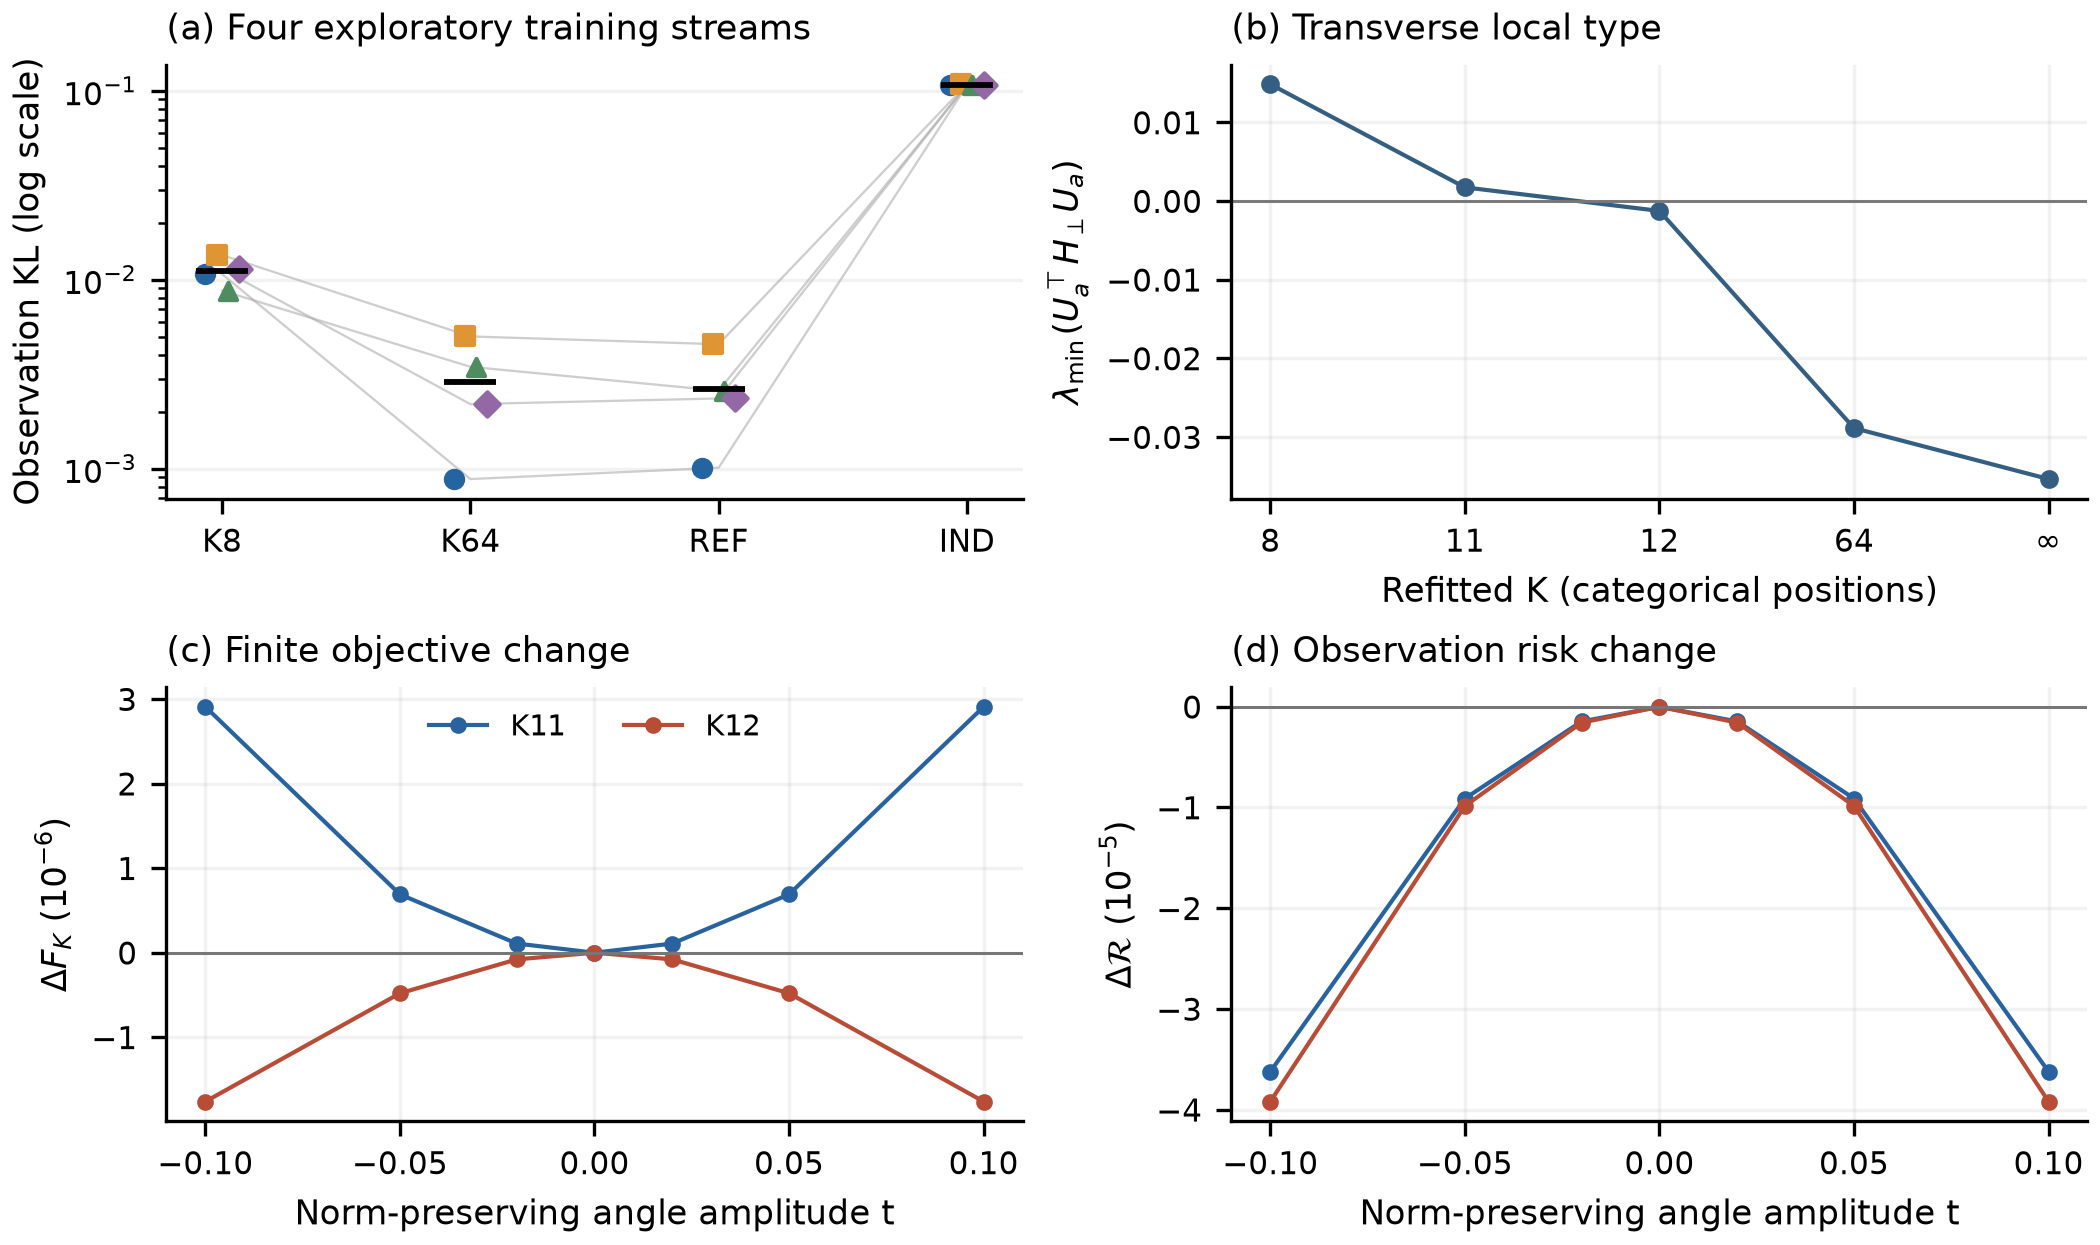
\includegraphics[width=1\linewidth,height=\textheight,keepaspectratio,alt={Learning and local geometry. (a) Observation KL for four independent streams on a logarithmic scale; black bars are means. (b) Minimum Cartesian transverse curvature, excluding common rotation, after refitting at each particle count; these are not angular eigenvalues or a continuous bifurcation. (c,d) K11/K12 objective and risk changes in nats per observation along d\_\{\textbackslash mathrm\{ang\}\}\^{}\{(12)\}, with biases and row lengths fixed. These small numerical effects differ from the same-root K8 certificate (14)--(15).}]{figures/joint_mechanism.png}
\caption{Learning and local geometry. (a) Observation KL for four
independent streams on a logarithmic scale; black bars are means. (b)
Minimum Cartesian transverse curvature, excluding common rotation, after
refitting at each particle count; these are not angular eigenvalues or a
continuous bifurcation. (c,d) K11/K12 objective and risk changes in nats
per observation along \(d_{\mathrm{ang}}^{(12)}\), with biases and row
lengths fixed. These small numerical effects differ from the same-root
K8 certificate (14)--(15).}
\end{figure}

\subsection*{I.8. Certified population local minimum and risk
conflict}\label{proof-theorem-3}

This section proves Theorem 3 for the exact population objective (I.1),
at K8. The witness is a genuine stationary point of the expectation
objective, located by inclusion rather than by treating the printed
numerical endpoint as an exact root. The teacher, the centre and every
norm in the argument refer to the same model.

\protect\phantomsection\label{full-local-statement}
\textbf{Full quantitative statement of Theorem 3.}

\textbf{(i) Full-space local minimum and positive risk.}

For the exact teacher in (13), let \(q_*\) be its observation law and
\(\mathcal R(\theta)=D(q_*\Vert Q_\theta)\). There exist a collinear
interior parameter \(\theta_*=(0,a_*,0)\) with \(a_{*,i}>0\) and a fixed
physical unit direction \(d_{\mathrm{risk}}\in\mathbb R^{24}\) such that
\(\theta_*\) is a strict local minimum of \(F_8^{q_*}\) in the full
24-dimensional parameter space modulo common latent rotations. For the
exact dyadic center \(\theta_0\) specified in
\hyperref[proof-theorem-3]{Appendix I.8},

\[
\begin{gathered}
\|\theta_*-\theta_0\|_2<1.805\times10^{-8},\\
\nabla F_8^{q_*}(\theta_*)=0,\qquad
D\mathcal R(\theta_*)[d_{\mathrm{risk}}]<-.0201723.
\end{gathered}
\]

Every observation marginal is correct,
\(Q_{\theta_*}(Y_j=1)=q_*(Y_j=1)=1/2\), while
\(0.0104335716\le\mathcal R(\theta_*)\le0.0104335744\). The fixed
\(10^{-7}\) step along \(d_{\mathrm{risk}}\) raises \(F_8\) and strictly
lowers risk while preserving these observation marginals; row lengths
and Gaussian logit variances change.

\Needspace{5\baselineskip}

\textbf{(ii) Same-root angular conflict.}

There is also a fixed
\(d=d_{\mathrm{ang}}^{(8)}\in\mathbf1^\perp\subset\mathbb R^8\),
\(\|d\|_2=1\), such that the path \(\theta_{\mathrm{ang}}(t)=(0,W(t))\)
satisfies

\[
\begin{aligned}
W_i(t)&=a_{*,i}\bigl(\cos(td_i),\sin(td_i)\bigr),\\
r(t)&=\mathcal R(\theta_{\mathrm{ang}}(t)),\\
r'(0)&=0,\qquad r''(0)<-.00450377.
\end{aligned}
\]

There exists \(\varepsilon>0\) such that, for every
\(0<|t|<\varepsilon\),

\[
\begin{gathered}
F_8^{q_*}(\theta_{\mathrm{ang}}(t))>F_8^{q_*}(\theta_*),\\
\mathcal R(\theta_{\mathrm{ang}}(t))<\mathcal R(\theta_*),\\
\operatorname{rank}W(t)=2.
\end{gathered}
\]

The path preserves all row lengths, logit marginals \(N(0,a_{*,i}^2)\)
and fair observation marginals. Its unit normalization is in angle
space, not in Cartesian path velocity. The preserved candidate logit
variances differ from the teacher's \(.8^2\).

\subsubsection*{I.8.1. Exact inputs, symmetry and the full parameter
space}\label{i.8.1.-exact-inputs-symmetry-and-the-full-parameter-space}

The teacher length and angles are exact rationals. The candidate centre
is an exact dyadic interpretation of the paired symmetrization of the
old population endpoint. Its positive first four row lengths are
specified below, and the remaining four are their reversal. The centre
is not reoptimized. Write the loading columns as u and v; vectors use
physical Euclidean norms and matrices use operator norms.

\[
\begin{aligned}
W_{*,j}&=\tfrac45(\cos\phi_{*,j},\sin\phi_{*,j}),\quad b_*=0,\quad
\phi_*=(-\tfrac7{10},-\tfrac12,-\tfrac3{10},-\tfrac1{10},\tfrac1{10},\tfrac3{10},\tfrac12,\tfrac7{10}),\\
\theta_0&=(0,a_0,0),\qquad a_{0,j}=a_{0,9-j},\\
(a_{0,1},\ldots,a_{0,4})&=
\left(\frac{4236614515730759}{9007199254740992},
\frac{1274451243427741}{2251799813685248},
\frac{181129089615167}{281474976710656},
\frac{775431105319425}{1125899906842624}\right).
\end{aligned}
\tag{I.21}
\]

Let P reverse the eight observations. The teacher satisfies
label-complement symmetry and reversal symmetry: the latter reverses the
sign of its second latent coordinate. Simultaneously complementing
labels and all latent particles proves whole-vector bias evenness, not
separate evenness of each bias. Reflection of the second latent
coordinate is valid for every target. Consequently, with four isometric
coordinates,

\[
\begin{aligned}
q_*(\mathbf1-y)&=q_*(y)=q_*(Py),\qquad
F_8^{q_*}(-b,W)=F_8^{q_*}(b,W),\\
F_8^q(b,u,-v)&=F_8^q(b,u,v),\qquad
U_+=\frac1{\sqrt2}(e_1+e_8,e_2+e_7,e_3+e_6,e_4+e_5),\\
a&=U_+\xi,\qquad f(\xi)=F_8^{q_*}(0,U_+\xi,0),\qquad
\nabla_bF_8^{q_*}=\nabla_vF_8^{q_*}=0,\quad \nabla_aF_8^{q_*}=U_+\nabla f.
\end{aligned}
\tag{I.22}
\]

The last line holds on the paired zero-bias, collinear subspace. It
gives equality of the four-coordinate and full 24-coordinate gradient
norms. It does not reduce the local-type test to four directions: the
test retains eight biases, four symmetric and four antisymmetric
row-length directions, and seven nonrotation transverse directions. All
Hessians below are differentiated in the unconstrained full model before
evaluation at the paired centre.

For computation only, a label has four paired counts. Gaussian particle
reflection identifies each count with its complement, leaving 41
lexicographically chosen representatives. Original teacher probabilities
are summed into these classes. The teacher is not assumed exchangeable
within individual pairs.

\[
\begin{aligned}
c_j&=y_j+y_{9-j}\in\{0,1,2\},\qquad
A_c(z)=\prod_{j=1}^4\sigma(a_{0,j}z)^{c_j}[1-\sigma(a_{0,j}z)]^{2-c_j},\\
G_{\xi,c}(z)&=\frac z{\sqrt2}\{c-2\sigma(a_{0,1:4}z)\},\qquad
A_{2-c}(-z)=A_c(z),\quad G_{\xi,2-c}(-z)=G_{\xi,c}(z),\\
\mu_c&=-E\sum_{k=1}^8\pi_kG_{\xi,c}(Z_k)=\mu_{2-c},\qquad
\nabla f=\sum_{r\in\mathcal C}w_r\mu_r,\\
\mathcal C&=\{\min(c,2-c):c\in\{0,1,2\}^4\},\quad|\mathcal C|=41,\quad
w_r=\sum_{y:\min(c(y),2-c(y))=r}q_*(y).
\end{aligned}
\tag{I.23}
\]

The equality of class gradients uses the sign-reflected Gaussian bank,
not an unchanged fixed bank. For Hessians the full label residual must
be retained.

\subsubsection*{I.8.2. The Hessian density that is actually
integrated}\label{i.8.2.-the-hessian-density-that-is-actually-integrated}

Set the likelihood scale to one and use the physical Laplace variable.
With the full 16-coordinate score and conditional negative Hessian from
(I.6), define the following inner moments; all expectations are
one-dimensional standard Gaussian expectations at the collinear point.
Here \(B=B_y(z)\) is the single-particle conditional negative Hessian,
whereas \(\mathcal B=\mathcal B_y(v)\) is its \(t\)-weighted Gaussian
moment; the label and auxiliary-coordinate dependence is suppressed in
(I.24).

\[
\begin{aligned}
u&=e^v,\quad t=uA_y(z)e^{-uA_y(z)},\quad\Psi=E e^{-uA_y(Z)},\quad T_0=Et,\\
\mathcal R&=E[tG],\quad\mathcal Q=E[tGG^\top],\quad\mathcal B=E[tB],\quad
\mathcal Q_p=E[trr^\top],\quad\mathcal B_p=E[t\operatorname{diag}\sigma'(a_0Z)],\\
I_{ba,y}(v)&=K\Psi^{K-1}\mathcal B-K(K-1)\Psi^{K-2}(T_0\mathcal Q-\mathcal R\mathcal R^\top),\\
I_{p,y}(v)&=K\Psi^{K-1}\mathcal B_p-K(K-1)\Psi^{K-2}T_0\mathcal Q_p,\qquad K=8.
\end{aligned}
\tag{I.24}
\]

Integrating these densities over the real auxiliary axis and averaging
over labels gives the complete radial and transverse blocks. The first
term is the conditional negative Hessian. The second term contains the
same-particle contribution minus the distinct-particle score outer
product. In the transverse block the latter vanishes because different
particles have independent, centred second coordinates. The identities
for the reciprocal and squared reciprocal in I.3 supply the displayed
powers and factors; there is no additional scaling by K or u.

One must distinguish this same/distinct-particle density from direct
parameter differentiation of the gradient density. For a real bank put
the sum and likelihood weights below; the resulting covariance is
positive semidefinite.

\[
\begin{aligned}
S&=\sum_kA_k,\quad w_k=A_k/S,\quad s=e^vS,\\
\bar B&=\sum_kw_kB_k,\quad\bar G=\sum_kw_kG_k,\quad\bar Q=\sum_kw_kG_kG_k^\top,\\
I_{ba}(v)&=E[e^{-s}\{s\bar B-s^2(\bar Q-\bar G\bar G^\top)\}],\\
I_{\rm dir}(v)&=E[e^{-s}\{s(\bar B-\bar Q)+s^2\bar G\bar G^\top\}],\\
I_{ba}(v)-I_{\rm dir}(v)&=E[\partial_v(se^{-s})\bar Q],\\
\int_{\mathbb R}(I_{ba}-I_{\rm dir})\,dv&=0.
\end{aligned}
\tag{I.25}
\]

The boundary term is zero for each positive bank sum, with Gaussian
score moments justifying exchange of expectation and integration. The
densities have the same full real integral but different finite-grid
values. The error envelopes below apply to the first density, which is
the one used for the certificate.

For a complement-side label use its effective label complement, while
the self-complement count is included once. This preserves the three
diagonal blocks; the bias--radial mixed block changes sign and is zero
only after using exact teacher symmetry. For each representative form
weighted label moments and inner probability moments:

\[
\begin{aligned}
W&=\sum q_y,\quad M_i=\sum q_y\widetilde y_i,\quad S_{ij}=\sum q_y\widetilde y_i\widetilde y_j,\\
T_l&=E[tz^l],\quad P_{l,i}=E[tz^lp_i(z)],\quad PP_{l,ij}=E[tz^lp_i(z)p_j(z)],\quad p_i(z)=\sigma(a_{0,i}z),\\
D_l&=W\operatorname{diag}(P_l-\operatorname{diag}PP_l),\quad l=0,2,\\
J_{bb}&=W(T_0PP_0-P_0P_0^\top),\\
J_{aa}&=(T_0T_2-T_1^2)S-T_0(MP_2^\top+P_2M^\top)
+T_1(MP_1^\top+P_1M^\top)+W(T_0PP_2-P_1P_1^\top),\\
J_p&=T_0(T_0S-MP_0^\top-P_0M^\top+WPP_0),\\
I_{bb}&=K\Psi^{K-1}D_0-K(K-1)\Psi^{K-2}J_{bb},\quad
I_{aa}=K\Psi^{K-1}D_2-K(K-1)\Psi^{K-2}J_{aa},\\
I_p&=K\Psi^{K-1}D_0-K(K-1)\Psi^{K-2}J_p.
\end{aligned}
\tag{I.26}
\]

The label moments cancel algebraically in the first covariance
difference, but remain in the other two. They are eight-coordinate
vectors and matrices; no division by class mass is used. Four distinct
probabilities reduce the inner scalar moment count to 36 including the
Laplace transform, without reducing any Hessian dimension. This retains
the information needed for broken-pair and antisymmetric row-length
directions.

\subsubsection*{I.8.3. Interval quadrature, discrete tails and
composition}\label{i.8.3.-interval-quadrature-discrete-tails-and-composition}

The computation uses 192-bit midpoint-radius arithmetic
\citep{johansson2017}. Finite sums are enclosed by their exact dyadic
endpoints. They are then enlarged by analytic infinite-grid and
omitted-grid errors. Agreement between floating-point rules is not used
as an error bound. For an analytic strip with vanishing contour edges
and integrable boundary envelopes, Fourier contour shift followed by
Poisson periodization gives \citep{trefethen2014}

\[
\left\|\int_{\mathbb R}f(x)\,dx-h\sum_{k\in\mathbb Z}f(kh)\right\|
\le\frac{M_++M_-}{e^{2\pi d/h}-1},\qquad
M_\pm\ge\int_{\mathbb R}\|f(x\pm id)\|\,dx.
\tag{I.27}
\]

The same argument holds for vector Euclidean and matrix operator norms.
In this model all real-axis derivatives have Gaussian-polynomial or
auxiliary rapid-decay envelopes, so the real functions are Schwartz;
absolute convergence of the Fourier series also verifies the
periodization identity. Analyticity alone would not suffice.

For the teacher the grid is the full-weight two-dimensional lattice on
the stated rectangle. In its polystrip each logit avoids sigmoid poles,
and the sum of absolute likelihoods over all labels factorizes. This
bounds the complete probability vector without multiplying a per-label
bound by 256.

Specifically, \(\sum_y|A_y(x+it)|\le\prod_j\sec(B_j/2)\), and
\(|\varphi(x_i+it_i)|=e^{t_i^2/2}\varphi(x_i)\). Fourier shifts in the
two coordinates give the product of their geometric alias sums; deleting
the zero frequency gives the factor in the next formula.

\[
\begin{aligned}
\theta_{\rm T}&=(b_*,W_*),\quad h_t=\tfrac18,\quad L_t=10,\quad d_t=1,\\
q_y^f&=h_t^2\sum_{|k_1|,|k_2|\le80}\varphi(h_tk_1)\varphi(h_tk_2)A_y(h_tk;\theta_{\rm T}),\\
B_j&=d_t(|W_{*,j1}|+|W_{*,j2}|)<\pi,\quad
M_t=e^{d_t^2}\prod_j\sec(B_j/2),\quad \rho_t=e^{-2\pi d_t/h_t},\\
\|q_*-q^f\|_1&\le\delta_t:=M_t\frac{4\rho_t}{(1-\rho_t)^2}
+2(1+h_t\varphi(0))\frac{2\varphi(L_t)}{L_t}<4.894\,10^{-21}.
\end{aligned}
\tag{I.28}
\]

The second term is an omitted-lattice Gaussian mass bound: the infinite
one-axis mass is at most one plus the central grid weight, and each
omitted right tail is bounded by its adjacent continuous tail. All
retained edges and corners have full weights. Finite-sum arithmetic
radii are retained separately in the probability balls.

The candidate inner and outer grids, including full endpoint weights,
are fixed as follows. Set the total loading sum, sector angle and secant
constants below. Each sigmoid factor has argument between zero and its
logit imaginary part, so the likelihood product has a continuous
argument bounded by the sector angle. Hence its real part is positive in
the inner strip, uniformly for every real auxiliary coordinate.

\[
\begin{aligned}
h_z&=\tfrac1{40},\ L_z=11,\ d_z=\tfrac18,\qquad
h_v=\tfrac18,\ v_-=-32,\ v_+=64,\ d_v=\tfrac12,\ W_v=96.125,\\
C_a&=\sum_i|a_{0,i}|,\quad\beta=C_ad_z<\pi/2,\quad
c_i=\sec(|a_{0,i}|d_z/2),\ C_R^2=\sum_i c_i^2,\ c_*^2=\max_i c_i^2,\\
\operatorname{Re}A_y(x+it)&\ge|A_y(x+it)|\cos\beta>0,\quad
|e^{-uA_y}|\le1,\quad |uA_ye^{-uA_y}|\le(e\cos\beta)^{-1},\\
F_z&=\frac{e^{d_z^2/2}}{e\cos\beta},\quad J_z=2+d_z^2,\quad
\rho_z=e^{-2\pi d_z/h_z},\qquad
\delta_X=\frac{2M_X\rho_z}{1-\rho_z}+T_X.
\end{aligned}
\tag{I.29}
\]

There are 881 inner nodes and 769 outer nodes. On the strip, residual
norms and conditional-Hessian norms are bounded by the secants; Gaussian
boundary integration gives the following envelopes. The middle column is
a scalar, vector or operator boundary-integral bound as appropriate; the
last column is an omitted-inner-grid bound.

The finite-sum implementation can enclose \(e^{-x}\) and \(xe^{-x}\) by
\([0,e^{-128}]\) and \([0,128e^{-128}]\) when the interval input proves
\(x=uA\ge128\). These are conservative saturation intervals, not
substituted zero values; their radii remain in the final finite-sum
boxes.

\begin{longtable}[]{@{}lll@{}}
\toprule\noalign{}
Moment & \(M_X\) & \(T_X\) \\
\midrule\noalign{}
\endhead
\bottomrule\noalign{}
\endlastfoot
\(\Psi\) & \(e^{d_z^2/2}\) & \(p_L\) \\
\(T_0\) & \(F_z\) & \(p_L/e\) \\
\(\mathcal R\) & \(F_z\sqrt{C_R^2J_z}\) &
\(2\sqrt{2m}\varphi(L_z)/e\) \\
\(\mathcal Q\) & \(F_z C_R^2J_z\) & \(m j_L/e\) \\
\(\mathcal B\) & \(F_z c_*^2J_z/4\) & \(j_L/(4e)\) \\
\(\mathcal Q_p\) & \(F_z C_R^2\) & \(m p_L/e\) \\
\(\mathcal B_p\) & \(F_z c_*^2/4\) & \(p_L/(4e)\) \\
\end{longtable}

The tail symbols are \(p_L=2\varphi(L_z)/L_z\) and
\(j_L=2\varphi(L_z)(L_z+2/L_z)\), with \(m=8\). They follow from
monotone right-rectangle comparison beyond the retained endpoint,
including the first and second Gaussian moments. Ordinary transposes,
not conjugate transposes, occur in the analytic density; complex
rank-one matrices still satisfy the operator bound by the squared vector
norm.

Uniform inner errors propagate through the nested powers and matrix
products. For this estimate only, let lower-case letters denote upper
bounds on the true moment norms, and use the following product-error
operator.

\[
\begin{aligned}
P&=1+\delta_\Psi,\quad
\mathcal E_n(b,\delta b)=P^n\delta b+nP^{n-1}\delta_\Psi b,\\
C&=T_0\mathcal Q-\mathcal R\mathcal R^\top,\quad
\|C\|\le tq+r^2,\quad
\delta_C\le\delta_{T_0}q+(t+\delta_{T_0})\delta_{\mathcal Q}+2r\delta_{\mathcal R}+\delta_{\mathcal R}^2,\\
C_p&=T_0\mathcal Q_p,\quad\|C_p\|\le tq_p,\quad
\delta_{C_p}\le\delta_{T_0}q_p+(t+\delta_{T_0})\delta_{\mathcal Q_p},\\
E_{{\rm in},ba}&=W_v\{K\mathcal E_{K-1}(b,\delta_{\mathcal B})
+K(K-1)\mathcal E_{K-2}(tq+r^2,\delta_C)\},\\
E_{{\rm in},p}&=W_v\{K\mathcal E_{K-1}(b_p,\delta_{\mathcal B_p})
+K(K-1)\mathcal E_{K-2}(tq_p,\delta_{C_p})\}.
\end{aligned}
\tag{I.30}
\]

The factor \(W_v=769h_v=96.125\) is the total weight of the finite outer
sum, including full endpoint weights. The terms \(E_{{\rm in},ba}\) and
\(E_{{\rm in},p}\) compare exact and approximated inner moments within
this finite sum; outer alias and omitted-grid tails are bounded
separately.

The valid real-axis bounds are \(t=1/e\), \(r=\sqrt{2m}/e\), \(q=2m/e\),
\(b=1/(2e)\), \(q_p=m/e\), and \(b_p=1/(4e)\). Telescoping powers and
the matrix triangle inequality prove (I.30); no factor close to one is
silently removed. The four-gradient computation uses the same argument
for \(D=E[tG_\xi]\), with \(\|D\|\le E_G/e\) and the following vector
envelope.

\[
\begin{aligned}
E_G&=\sqrt m\sqrt{2/\pi},\quad
M_D=F_z\sqrt{C_R^2(1+d_z^2)},\quad
\delta_D=\frac{2M_D\rho_z}{1-\rho_z}+2\sqrt m\varphi(L_z)/e,\\
E_{{\rm in},g}&=KW_v\{P^{K-1}\delta_D+(K-1)P^{K-2}\delta_\Psi E_G/e\}.
\end{aligned}
\tag{I.31}
\]

For the outer strip, real-bank likelihood weights remain real; only the
auxiliary scalar becomes complex. Integrating the absolute bank
densities after the change of variable to the bank-scaled auxiliary
radius gives

\[
\begin{aligned}
M_{ba}&=(1+K)\{(4\cos d_v)^{-1}+m(\cos d_v)^{-2}\},\\
M_p&=(4\cos d_v)^{-1}+m(\cos d_v)^{-2},\quad M_g=KE_G/\cos d_v,\\
E_{{\rm alias},X}&=\frac{2M_X\rho_v}{1-\rho_v},\qquad
\rho_v=e^{-2\pi d_v/h_v},\quad X\in\{ba,p,g\}.
\end{aligned}
\tag{I.32}
\]

At the lower end, the densities and their derivatives decay
exponentially. At the upper end split Gaussian banks at a latent
threshold proportional to the auxiliary coordinate: on the
bounded-latent part the likelihood sum gives double-exponential decay;
on its complement Gaussian tails give rapid decay. Differentiating
produces polynomials in the bank-scaled auxiliary radius times its
damped exponential, so the same split applies at every fixed derivative
order. This establishes the contour-edge and Schwartz conditions for the
outer use of (I.27).

Omitted outer points require discrete-tail bounds. For the two bank
kernels, the total variations below control a right-grid tail by its
continuous integral plus a mesh-times-variation term. If the boundary is
already past the peak, monotone right rectangles give the tighter
continuous bound.

\[
\begin{aligned}
f_1(v)&=se^{-s},\quad f_2(v)=s^2e^{-s},\quad
\int_{\mathbb R}|f_1'(v)|\,dv=2/e,\quad\int_{\mathbb R}|f_2'(v)|\,dv=8/e^2,\\
l_1&=\frac{h_ve^{v_-}}{e^{h_v}-1},\quad l_2=\frac{h_ve^{2v_-}}{e^{2h_v}-1},\quad
E_{{\rm low},p}\le Kl_1/4+mK^2l_2,\quad E_{{\rm low},ba}\le(1+K)E_{{\rm low},p},\\
T&=4,\quad U=e^{v_+},\quad\eta=2^{-m}e^{-C_aT},\quad U\eta>2,\\
p_T&=2\varphi(T)/T,\quad t_{2T}=2\varphi(T)(T+1/T),\quad
C_{\rm bad}=\tfrac14(1+2h_v/e)+m(1+8h_v/e^2),\\
G_p&=\{\tfrac14+m(1+U\eta)\}e^{-U\eta},\quad
E_{{\rm up},p}\le G_p+C_{\rm bad}p_T^K,\\
E_{{\rm up},ba}&\le(1+K)G_p+C_{\rm bad}(p_T^K+Kt_{2T}p_T^{K-1}).
\end{aligned}
\tag{I.33}
\]

Here \(Z_k\) is the scalar first latent coordinate used by the collinear
likelihood and its one-dimensional inner integration. Define
\(G=\{\min_{1\le k\le8}|Z_k|\le T\}\) and
\(G^c=\bigcap_{k=1}^8\{|Z_k|>T\}\). On \(G\), the likelihood sum
satisfies \(S=\sum_k A_y(Z_k)\ge\eta\). On \(G^c\), independence and
double-sided Gaussian tails give \(\Pr(G^c)\le p_T^K\) and
\(E[(1+M^2)\mathbf1_{G^c}]\le p_T^K+Kt_{2T}p_T^{K-1}\), where
\(M=\max_k|Z_k|\). Thus the mesh correction is retained on the bad set
rather than applying a continuous Laplace tail to every omitted lattice
point. For the gradient the corresponding bounds are

\[
\begin{aligned}
E_{{\rm low},g}&\le KE_Gl_1,\\
E_{{\rm up},g}&\le\sqrt m\{\sqrt K e^{-U\eta}+(1+2h_v/e)2K\varphi(T)p_T^{K-1}\}.
\end{aligned}
\tag{I.34}
\]

Sum the inner replacement, outer alias and the two discrete tails to
obtain a uniform error for each label. The finite teacher mass is at
most one plus its L1 error. The labelwise true gradient bound and
conservative Hessian bounds below transfer teacher error only once per
vector or matrix norm.

\[
\begin{aligned}
E_X^{\rm unif}&=E_{{\rm in},X}+E_{{\rm alias},X}+E_{{\rm low},X}+E_{{\rm up},X},\\
\|g_{\xi,y}\|&\le\sqrt m E\max_k|Z_k|\le\sqrt{mK}=8,\\
\|H_{ba,y}\|&\le(2m+\tfrac14)(1+K)=146.25,\quad\|H_{p,y}\|\le m+\tfrac14=8.25,\\
E_g&\le(1+\delta_t)E_g^{\rm unif}+8\delta_t,\quad
E_{ba}\le(1+\delta_t)E_{ba}^{\rm unif}+146.25\delta_t,\\
E_p&\le(1+\delta_t)E_p^{\rm unif}+8.25\delta_t.
\end{aligned}
\tag{I.35}
\]

For the Hessian, use each label's block-diagonal bias/radial principal
blocks and its transverse block; folding preserves exactly these
objects. The exact teacher mixed block is zero. Finite teacher
probabilities need not satisfy a bitwise symmetry test. The interval
finite matrices retain their weight and arithmetic uncertainty;
Frobenius upper bounds dominate operator norms when comparing them with
saved dyadic matrices.

The final outward-rounded bounds are as follows. The saved matrices are
exact dyadic interpretations of the previous symmetric binary64
matrices; their positivity is proved by interval LDL. A rational basis
of the fixed transverse slice is tested against its Gram matrix, rather
than assumed orthonormal.

The rational basis has columns \(V_j=e_j-(a_{0,j}/a_{0,8})e_8\),
\(1\le j\le7\). The test is \(V^\top(S_p-.014I)V\succ0\), which
certifies the physical curvature bound relative to \(V^\top V\).

\[
\begin{aligned}
\|\nabla F_8^{q_*}(\theta_0)\|_2&<7.572\,10^{-10},\\
\|H_{ba}(\theta_0)-S_{ba}\|_{\rm op}&<1.138\,10^{-8}<.001,\\
\|H_p(\theta_0)-S_p\|_{\rm op}&<2.531\,10^{-9}<.001,\\
S_{ba}&\succ.050I_{16},\qquad
w^\top S_pw>.014\|w\|_2^2\quad(0\ne w\perp a_0).
\end{aligned}
\tag{I.36}
\]

\begin{longtable}[]{@{}
  >{\raggedright\arraybackslash}p{(\linewidth - 6\tabcolsep) * \real{0.2000}}
  >{\raggedleft\arraybackslash}p{(\linewidth - 6\tabcolsep) * \real{0.2667}}
  >{\raggedleft\arraybackslash}p{(\linewidth - 6\tabcolsep) * \real{0.2667}}
  >{\raggedleft\arraybackslash}p{(\linewidth - 6\tabcolsep) * \real{0.2667}}@{}}
\toprule\noalign{}
\begin{minipage}[b]{\linewidth}\raggedright
Contribution
\end{minipage} & \begin{minipage}[b]{\linewidth}\raggedleft
Gradient L2
\end{minipage} & \begin{minipage}[b]{\linewidth}\raggedleft
Radial Hessian operator
\end{minipage} & \begin{minipage}[b]{\linewidth}\raggedleft
Transverse Hessian operator
\end{minipage} \\
\midrule\noalign{}
\endhead
\bottomrule\noalign{}
\endlastfoot
Inner replacement & 2.49106e−10 & 9.04057e−9 & 2.27090e−9 \\
Outer alias & 5.00387e−10 & 2.33628e−9 & 2.59587e−10 \\
Outer lower tail & 2.14647e−13 & 2.14005e−13 & 2.37783e−14 \\
Total mathematical error, including teacher & \textless7.497076e−10 &
\textless1.137708e−8 & \textless2.530514e−9 \\
Finite-box norm or distance to saved matrix & \textless7.490176e−12 &
\textless1.456e−13 & \textless2.663e−14 \\
\end{longtable}

Table decimals summarize bounds; exact dyadic endpoints and rational
comparisons determine (I.36). The omitted upper-tail contribution is
included in the total. No 41-class, 256-label or matrix-entry multiplier
is inserted into a bound already expressed in the corresponding vector
or operator norm.

\subsubsection*{I.8.4. Root inclusion and 23-direction local
minimality}\label{i.8.4.-root-inclusion-and-23-direction-local-minimality}

A uniform full-parameter Hessian variation bound turns the centre
certificate into a neighbourhood certificate. Let the bank envelope
below include both latent coordinates. Conditional log-kernel
derivatives of orders one, two and three are bounded by the stated
powers. Differentiating log-sum-exp gives a mean third derivative, three
covariance terms and a centred third moment; their bounds give the
displayed constant. Gaussian moments justify differentiation under
expectation.

\[
\begin{gathered}
q_Z=\sqrt{1+\max_{k\le K}\|Z_k\|^2},\\
\|D\ell_k\|\le\sqrt m q_Z,\quad\|D^2\ell_k\|\le q_Z^2/4,\quad\|D^3\ell_k\|\le q_Z^3/4,\\
L_F\le(\tfrac14+\tfrac32\sqrt m+8m^{3/2})
[1+2dK+dK(dK+2)]^{3/4}<14069,\quad m=K=8,\ d=2,\\
\|H_F(\theta)-H_F(\theta')\|_{\rm op}\le14069\|\theta-\theta'\|_2.
\end{gathered}
\tag{I.37}
\]

For example each covariance term is at most twice the product of the
first- and second-derivative bounds, and the centred third moment is at
most eight times the cube of the first bound. The bank's squared
envelope is dominated by one plus a chi-square variable with sixteen
degrees of freedom. The integer cap is checked by rational upper bounds,
not fitted from numerical derivatives. With the preassigned physical
radius,

\[
\begin{aligned}
r&=5\,10^{-7},\qquad
m_r=m_{16}=.050-.001-14069r=.0419655,\\
m_T&=.014-.001-14069r=.0059655,\qquad
\epsilon_g=7.572\,10^{-10}<m_rr=2.098275\,10^{-8}.
\end{aligned}
\tag{I.38}
\]

The four-coordinate closed ball has a strongly convex restricted
objective. On its sphere, integrating the Hessian along the
centre-to-boundary line gives the outward inequality below. A
closed-ball minimum cannot lie on the boundary, since an inward move
would decrease the objective. It is therefore an interior restricted
root, unique within this ball by strong convexity. Exact symmetry in
(I.22) lifts it to a full stationary point. Strong monotonicity further
gives its location.

\[
\begin{aligned}
\delta^\top\nabla f(\xi_0+\delta)&\ge-\epsilon_g r+m_rr^2>0\quad(\|\delta\|=r),\\
\nabla F_8^{q_*}(\theta_*)&=0,\qquad\theta_*=(0,a_*,0),\qquad
\|\theta_*-\theta_0\|_2<\epsilon_g/m_r<1.805\,10^{-8}.
\end{aligned}
\tag{I.39}
\]

The fixed slice is \(a_0^\top v=0\). The derivative of this constraint
along a common latent rotation is \(a_0^\top u\), positive throughout
the small neighbourhood. The implicit function theorem gives a unique
small rotation taking any nearby point into the slice. At the true root,
reflection makes the radial/transverse mixed blocks zero; (I.38) makes
its 16 radial and seven slice-transverse directions positive. Taylor's
theorem gives a strict slice minimum, and rotation invariance lifts it
to a strict local minimum modulo common rotation. The 24-dimensional
Hessian is singular along the common-rotation direction, as rotation
invariance requires; the strict minimum is modulo that rotation, with
the 16 bias/radial and seven transverse directions certified positive.

\subsubsection*{I.8.5. Risk direction, fixed small step and
scope}\label{i.8.5.-risk-direction-fixed-small-step-and-scope}

The same centre and a fixed paired dyadic vector define the mathematical
unit direction \(d_{\mathrm{risk}}\in\mathbb R^{24}\). Candidate
probabilities and their directional derivatives are enclosed by 177
one-dimensional full-weight nodes with spacing one eighth on the
interval from minus eleven to eleven. Strip and Gaussian-tail errors are
added; teacher probability errors transfer through the posterior ratios.
Jensen's inequality supplies a uniform positive probability bound on the
physical ball, and the posterior negative-Hessian identity bounds risk
curvature.

The direction-defining vector \(h\) in (I.40) differs from the grid
spacings \(h_t,h_z,h_v\) and the generic scalar mesh in (I.27). Its
entries come from pair symmetrization of a numerical radial risk
gradient; certification uses the fixed exact dyadics without assuming
equality to the true gradient. Its first four components are the
following exact dyadics; set \(h_{9-j}=h_j\) and use the mathematical
norm \(\|h\|_2=\sqrt{\sum_{j=1}^8h_j^2}\).

\begin{longtable}[]{@{}ll@{}}
\toprule\noalign{}
Component & Exact dyadic \\
\midrule\noalign{}
\endhead
\bottomrule\noalign{}
\endlastfoot
\(h_1\) & \(-8589911184852041/1152921504606846976\) \\
\(h_2\) & \(-2443582330405755/288230376151711744\) \\
\(h_3\) & \(-5282230754430109/576460752303423488\) \\
\(h_4\) & \(-2739850785036709/288230376151711744\) \\
\end{longtable}

\[
\begin{aligned}
d_{\mathrm{risk}}&=(0,-h/\|h\|_2,0),\\
B_{h,y}&=E[A_y(Z)Z\sum_i h_i\{y_i-\sigma(a_{0,i}Z)\}],\\
DR(\theta_0)[d_{\mathrm{risk}}]&=\sum_yq_*(y)\frac{B_{h,y}}{Q_y(\theta_0)\|h\|_2}\\
&\in[-.024564580310120128,-.024564580310120124],\\
Q_y(\theta)&\ge q_{\min}:=2^{-8}
\exp\{-3r/2-[r^2+(\|a_0\|_2+r)^2]/8\},\\
\|H_R(\theta)\|&\le M_R:=24/q_{\min}<8784.371,\\
DR(\theta)[d_{\mathrm{risk}}]&<-\nu,\quad\nu=.0201723,\qquad\|\theta-\theta_0\|_2\le r.
\end{aligned}
\tag{I.40}
\]

The numerator \(B_{h,y}\) is the derivative of \(Q_y\) along
\(+(0,h,0)\), so \(DQ_y(\theta_0)[d_{\mathrm{risk}}]=-B_{h,y}/\|h\|_2\).
The negative log probability in the risk contributes a second minus
sign, giving the positive sign in (I.40).

For completeness, the candidate probability and numerator boundary norms
in a width-one strip are at most the Gaussian shift factor times the
product of loading secants, and this quantity times the secant-weighted
absolute direction sum times square root of two, respectively. Formula
(I.27) bounds their lattice errors; omitted tails are at most twice the
Gaussian endpoint density divided by the endpoint, and twice that
density times the absolute direction sum. Positive probability lower
bounds permit interval division. The teacher L1 allowance multiplies the
largest absolute posterior ratio once.

To verify the curvature bound, a label's negative-log-probability
Hessian is the posterior mean conditional negative Hessian minus the
posterior score covariance. Both terms are positive semidefinite, so
their difference has norm at most the larger individual norm. The
likelihood is at most one; dividing prior score moments by the uniform
probability lower bound gives the stated bound. The direction is not
selected after evaluating the root.

The preassigned step remains inside the certified ball even when started
at the unknown exact root. It preserves zero biases, hence each observed
Bernoulli marginal is exactly fair by Gaussian central symmetry, while
row logit variances change with the row lengths. It is not the
fixed-row-norm angular path of I.7. Radial curvature and the uniform
risk derivative give

\[
\begin{aligned}
t&=10^{-7},\quad \|\theta_*-\theta_0\|_2+t<r,\\
F_8^{q_*}(\theta_*+td_{\mathrm{risk}})-F_8^{q_*}(\theta_*)&\ge\tfrac12m_{16}t^2=2.098275\,10^{-16}>0,\\
R(\theta_*)-R(\theta_*+td_{\mathrm{risk}})&>\nu t=2.01723\,10^{-9},\qquad
R(\theta_*)>2.01723\,10^{-9}.
\end{aligned}
\tag{I.41}
\]

This is an analytic consequence of the certified neighbourhood, not a
subtraction of nearly equal float64 losses. It certifies a strict
conflict at one population local minimum, not the size of a typical
training improvement. The positivity of KL proves the final inequality.

\textbf{Risk magnitude from stored probability intervals.} The preceding
small-step bound remains the core existence certificate. The teacher and
candidate probability intervals also allow a deterministic KL enclosure
at the centre and its transfer to the exact root. The observed score
information is bounded by the complete-data information, so the
following derivative bound uses only probability ratios.

\[
\begin{aligned}
\chi^2(q_*\Vert Q_0)&=\sum_y\frac{(q_*(y)-Q_y(\theta_0))^2}{Q_y(\theta_0)},\quad
I_{\rm obs}(\theta_0)\preceq I_{\rm complete}(\theta_0)\preceq\tfrac14I_{24},\\
\|\nabla R(\theta_0)\|_2&\le\tfrac12\sqrt{\chi^2(q_*\Vert Q_0)},\\
|R(\theta_*)-R(\theta_0)|&\le\tfrac12\sqrt{\chi^2(q_*\Vert Q_0)}\,\eta_*+\tfrac12M_R\eta_*^2,\quad
\eta_*=\epsilon_g/m_r.
\end{aligned}
\tag{I.42}
\]

Indeed the conditional complete-data score has cross-row information
zero and within-row information at most one quarter times the expected
outer product of the augmented Gaussian input, which is the identity.
Conditional expectation gives the observed score, decreasing information
by Jensen's inequality. Its model-probability-weighted mean is zero;
Cauchy--Schwarz applied to the target-minus-model weights then yields
(I.42). No target probability is renormalized, and no old floating-point
gradient is substituted for the full gradient norm.

Endpoint-only interval composition gives a centre risk about
0.01043357299286302, chi-square divergence about 0.021791388777069481, a
full gradient bound below 0.073809534, and a root-transfer allowance
below 1.334e−9. Outward rational rounding yields the rigorous enclosure

\[
R(\theta_*)\in[.0104335716,\ .0104335744].
\tag{I.43}
\]

This additional bound is a deterministic composition of saved
probability intervals and the certified root distance, with no new
integral, fit or random sample. It explains why the conservative
positive-risk lower bound in (I.41) should not be read as the actual
risk magnitude.

The evidence consists of complete interval finite sums plus the analytic
errors above. Independent alternative implementations recomputed eight
selected teacher labels over their full grid and two of the 41
gradient/Hessian classes over their full grids; this is not independent
recomputation of every class. All endpoint uncertainties enter the final
certificates. The earlier empirical fits, weak-loading K2 precision
failures, K11/K12 numerical continuation and mixed profile comparisons
retain their original scope. The result does not certify a globally
optimal solution, an optimizer's probability of entering the
neighbourhood, a universal critical K, or numerical detectability of the
tiny guaranteed finite step.

\subsection*{I.9. Qualitative stability under target
perturbations}\label{local-persistence}

\textbf{Corollary I.1 (qualitative teacher-law persistence).} There is a
neighbourhood of the exact teacher probability vector in the interior of
the probability simplex such that every target in that neighbourhood has
a nearby rank-one strict local minimum of its K8 objective modulo common
rotation, with negative integrated-risk derivative along the same fixed
direction \(d_{\mathrm{risk}}\in\mathbb R^{24}\). The perturbed
probabilities need not preserve complement or reversal symmetry. The
conclusion also holds for the distributions induced by all sufficiently
nearby teacher parameters in the original two-factor model. The
neighbourhood is not quantified.

\textbf{Proof.} Use all 23 coordinates on the fixed slice
\(\mathcal S=\{a_0^\top v=0\}\), not the four-coordinate symmetric
branch. Let \(E_{\mathcal S}\) have orthonormal columns spanning its
tangent space and use affine coordinates for probabilities summing to
one. The finite-particle objective is linear in the target and smooth in
the parameters, with Gaussian polynomial domination permitting each
derivative. At the certified root define

\[
\begin{aligned}
\mathcal F(s,q)&=E_{\mathcal S}^\top\nabla_\theta F_8^q(\theta_*+E_{\mathcal S}s),\\
\mathcal F(0,q_*)&=0,\qquad
D_s\mathcal F(0,q_*)=E_{\mathcal S}^\top H_F(\theta_*)E_{\mathcal S}\succ0.
\end{aligned}
\tag{I.44}
\]

The implicit function theorem gives a unique local smooth slice-critical
branch \(\theta(q)\). Take a sufficiently small slice neighbourhood
centred at \(\theta_*=(0,a_*,0)\) that is invariant under
\(T(b,u,v)=(b,u,-v)\) and lies inside the theorem's uniqueness
neighbourhood; shrink the target neighbourhood so that the branch
remains there. For every target, latent reflection leaves the objective
and the fixed slice invariant. The reflection of its slice-critical
point is therefore another slice-critical point in the same
neighbourhood. Uniqueness makes them equal. Continuity keeps \(u(q)\)
nonzero, so

\[
\begin{aligned}
F_8^q(T\theta)&=F_8^q(\theta),\qquad T\mathcal S=\mathcal S,\qquad T\theta(q)=\theta(q),\\
v(q)&=0,\qquad \operatorname{rank}W(q)=1.
\end{aligned}
\]

Slice criticality means that the ambient gradient is proportional to the
slice normal. Rotation invariance makes that gradient orthogonal to the
orbit tangent; the normal has nonzero product with this tangent because
the original transverse condition persists. Thus the ambient gradient is
zero, without imposing bias or paired-row constraints on the perturbed
target. Positive slice curvature persists by continuity, giving strict
local minimality modulo rotation.

\[
\begin{aligned}
\theta(q)&=\theta_*+E_{\mathcal S}s(q),\qquad
\nabla F_8^q(\theta(q))=0,\\
R_q(\theta)&=D_{\rm KL}(q\Vert p_\theta),\qquad
D R_q(\theta(q))[d_{\mathrm{risk}}]<0.
\end{aligned}
\tag{I.45}
\]

The final strict inequality follows by continuity of the directional
risk derivative, since all probabilities remain positive near the
interior teacher vector and the certified root. It also gives positive
risk. For the correctly specified teacher subclass, each observed
probability is continuous in the teacher parameters: its likelihood is
continuous and bounded by one, so dominated convergence applies. The
inverse image of the probability neighbourhood is thus a neighbourhood
of the original teacher parameters, and the conclusion holds there. This
does not assert that every nearby probability vector belongs to the
original two-factor model.

This is a qualitative consequence of nondegeneracy, not a new
teacher-grid experiment or a quantified applicability region. No
additional K range is claimed. The nearby branch remains rank one, while
its biases and paired row lengths need not retain their original
symmetry. In particular, the fair observation marginals at the original
root and along its certified risk step in I.8.5 are not asserted for
perturbed teachers or their roots.

\subsection*{I.10. A fixed-marginal angle conflict at the same exact
root}\label{same-root-angle}

We strengthen the witness in I.8 using its same exact teacher \(q_*\),
centre \(\theta_0=(0,a_0,0)\) and root \(\theta_*=(0,a_*,0)\). No root
is refitted. The new path changes relative angles while keeping every
row length fixed; it diagnoses the local minimum in the full model,
rather than imposing a constraint on the original learning problem.

\subsubsection*{I.10.1. Direction and full path
derivative}\label{i.10.1.-direction-and-full-path-derivative}

Define the integer vector and mathematical unit angle direction by

\[
\begin{aligned}
(u_1,u_2,u_3,u_4)&=(-8440215,-6758298,-4585241,-1673686),\\
u_{9-i}&=-u_i\quad(1\le i\le4),\qquad S=\sum_i u_i^2=281474961915412,\\
d=d_{\mathrm{ang}}^{(8)}&=u/\sqrt S,\qquad \|d\|_2=1,\qquad \mathbf1^\top d=0.
\end{aligned}
\tag{I.46}
\]

Saved numerical risk-angle information at the earlier P point motivated
this direction. Its exact construction was fixed before the new integral
evaluation and was not changed after evaluation; this is an exploratory
existence witness, not a blindly selected direction. All quadratic
coefficients use exact ratios such as \((u_i-u_j)^2/S\), without
rounding \(\sqrt S\). The angle normalization is distinct from unit
Cartesian path speed. This direction is also distinct from both
\(d_{\mathrm{risk}}\) in I.8.5 and \(d_{\mathrm{ang}}^{(12)}\) in
I.6--I.7.

For a collinear loading \(a\), let \(Z,X\) be independent standard
Gaussians and set \(\eta_i(t)=a_i\{Z\cos(td_i)+X\sin(td_i)\}\). Write
\(p_i(z)=\sigma(a_i z)\), \(r_i=y_i-p_i(z)\), \(D_i=p_i(1-p_i)\),
\(A_y(z)=\prod_i p_i^{y_i}(1-p_i)^{1-y_i}\) and \(Q_y=E A_y(Z)\). For
this paragraph define \(U=\sum_i a_i d_i r_i\),
\(V=\sum_i a_i d_i^2r_i\), \(G=\sum_i a_i r_i\) and
\(T=\sum_i a_i^2d_i^2D_i\). Differentiating the likelihood and
integrating out \(X\) gives

\[
\begin{aligned}
W_i(t)&=a_i(\cos(td_i),\sin(td_i)),\qquad b_i(t)=0,\\
\dot\eta_i(0)&=a_i d_iX,\qquad \ddot\eta_i(0)=-a_i d_i^2Z,\\
Q_y'(0)&=0,\qquad Q_y''(0)=E B_y(Z),\\
B_y(z)&=A_y(z)\{U^2-T-zV\}.
\end{aligned}
\tag{I.47}
\]

The first derivative vanishes by reflection in \(X\). In particular,
this is not a negative first-order risk direction. The acceleration term
\(-zV\) cannot be dropped: a Cartesian transverse Hessian alone
differentiates a different path. Bounded real sigmoid derivatives and
Gaussian polynomial envelopes justify these differentiations.

Set \(P_y(z)=\sum_{i<j}a_ia_j(d_i-d_j)^2r_ir_j\). Expansion gives
\(P_y=GV-U^2\), \(A_y'=A_yG\) and \(V'=-T\). Consequently

\[
\begin{aligned}
B_y+A_yP_y&=(A_yV)'-zA_yV
=\{\varphi A_yV\}'/\varphi,\\
Q_y''(0)&=-E[A_y(Z)P_y(Z)],\qquad N_y:=E[A_y(Z)P_y(Z)],\\
\mathcal H_R(a;d)&:=\left.\frac{d^2R(\theta(t))}{dt^2}\right|_{t=0}
=\sum_yq_*(y)\frac{N_y}{Q_y}
=\sum_yq_*(y)E_{\pi_y}P_y,\\
\pi_y(dz)&=A_y(z)\varphi(z)\,dz/Q_y.
\end{aligned}
\tag{I.48}
\]

Here \(\varphi A_yV\) vanishes at both real infinities because
\(A_y\le1\) and \(V\) is bounded. Thus the first line is a Gaussian
weighted total derivative, and the second line follows only after
integration. The integrands \(B_y\) and \(-A_yP_y\) are not asserted to
be equal pointwise. Differentiating the negative log probability
supplies the second minus sign; \(Q_y'(0)=0\) removes its
squared-first-derivative term. Constant \(d\) gives \(P_y=0\), as
required for common rotation.

\subsubsection*{I.10.2. Centre enclosure and an alternative path
expression}\label{i.10.2.-centre-enclosure-and-an-alternative-path-expression}

At the exact centre in (I.21), \(|a_{0,i}|<1\) and
\(\sum_{i<j}(d_i-d_j)^2=8\), so \(|P_y|\le8\). All 256 labels are
evaluated individually. On the closed strip
\(|\operatorname{Im}z|\le1\), set \(c=\sec(1/2)\). The inequality
\(|1+s e^{iv}|\ge(1+s)\cos(v/2)\) for \(s\ge0\), \(|v|\le1\), bounds
each complex Bernoulli factor by \(c\) times its real-axis value. Hence
\(|A_y|\le c^8\), \(|r_i|\le c\) and \(|D_i|\le c^2/4\). The two
numerator expressions have separate one-sided boundary-integral and
omitted-lattice bounds:

\[
\begin{aligned}
h&=1/8,\quad N=88,\quad L=Nh=11,\quad c=\sec(1/2),\\
M_{\rm pair}&=e^{1/2}c^8\,8c^2,\qquad M_Q=e^{1/2}c^8,\\
M_{\rm path}&=e^{1/2}c^8\{8c^2+c^2/4+c\sqrt2\},\\
T_{\rm pair}&=16\varphi(L)/L,\qquad T_Q=2\varphi(L)/L,\\
T_{\rm path}&=(8+1/4)2\varphi(L)/L+2\varphi(L),\\
\epsilon_j&=\frac{2M_j}{e^{2\pi/h}-1}+T_j,\qquad j\in\{{\rm pair},{\rm path},Q\}.
\end{aligned}
\tag{I.49}
\]

For the pair expression the integrand is \(\varphi A_yP_y\); for the
alternative it is \(-\varphi B_y\). On a strip boundary,
\(|U|\le\sqrt8c\), \(|T|\le c^2/4\), \(|V|\le c\) and
\(E|Z\pm i|\le\sqrt2\), which prove \(M_{\rm path}\). Contour
translation gives Fourier decay \(M_j e^{-|\xi|}\); summing the nonzero
Poisson frequencies proves the alias term, as in (I.27). The Gaussian
envelope makes the contour end boundaries vanish. On the real axis the
two numerator factors are bounded by \(8\) and \(8+1/4+|z|\),
respectively. The omitted full-weight nodes \(|k|>N\) are bounded by
adjacent continuous tails, using the monotonicity of \(\varphi(x)\) and
\(x\varphi(x)\) for \(x\ge L\ge1\). The identities
\(\int_L^\infty x\varphi(x)dx=\varphi(L)\) and
\(\int_L^\infty\varphi(x)dx\le\varphi(L)/L\) give the stated tails.

Each 177-node sum includes both endpoints with full weight and uses
192-bit Arb arithmetic. Its outward arithmetic interval is retained
separately from the analytic error. The pair error is approximately
\(1.44001098659947\,10^{-20}\) per label, not an error for the final
curvature. The alternative implementation forms the complete path
derivative in (I.47), retaining acceleration, with separate
integer-label probability products and its own bounds in (I.49); it also
recomputes \(Q_y\).

Let \([F_y]\) be the pair finite-sum interval and \([Q_y]\) the original
strictly positive true-probability enclosure used in I.8.5. Let
\(\widehat q_y\) be the exact midpoint of the two outward endpoints of
the saved teacher finite-sum interval. No normalization is applied to
these midpoints. The teacher certificate gives
\(\|q_*-\widehat q\|_1<\epsilon_q:=4.894\,10^{-21}\). Interval
composition is

\[
\begin{aligned}
[N_y]&=[F_y]+[-\epsilon_{\rm pair}^{\rm up},\epsilon_{\rm pair}^{\rm up}],\\
[\mathcal H_0]&=\sum_y\widehat q_y[N_y]/[Q_y]+[-8\epsilon_q,8\epsilon_q],\\
|N_y/Q_y|&=|E_{\pi_y}P_y|\le8,\qquad
8\epsilon_q=3.9152\,10^{-20}.
\end{aligned}
\tag{I.50}
\]

Here \(\epsilon^{\rm up}\) denotes a certified outward upper endpoint.
The teacher allowance occurs once, through the true posterior ratio
bound; the label-wise numerator error is propagated through division and
weighting. The alternative centre enclosure substitutes its path sum and
\(\epsilon_{\rm path}\), but uses the same old \([Q_y]\). Its newly
computed probabilities are a cross-check, not a different denominator
for this composition.

After their respective analytic enlargements, all 256 pairs of numerator
intervals overlap; all 256 recomputed probability intervals overlap
their old counterparts. These checks compare enclosures of equal
integrals, not identical finite sums, and do not replace the analytic
error proof. The implementations share Arb, teacher inputs and the root
certificate. A separate exact rational-arithmetic check recomposes saved
endpoints only; it does not recompute transcendental functions or
integrals. They are different-expression implementation checks, not
independent end-to-end certifications with different arithmetic
backends.

\subsubsection*{I.10.3. Scalar transfer to the certified
root}\label{i.10.3.-scalar-transfer-to-the-certified-root}

We require a variation bound for the one scalar \(\mathcal H_R(a;d)\) at
fixed \(q_*,b=0,d\), not a bound on the full risk Hessian. Suppose
\(\max_i|a_i|\le A\) along the segment in question, with \(m\) rows and
\(\|d\|_2=1\). Integrating \((zA_y\varphi)'\) over the real line gives

\[
\begin{aligned}
E_{\pi_y}Z^2&=1+E_{\pi_y}[Z\,\partial_z\log A_y],\qquad
|\partial_z\log A_y|\le mA,\\
\mu_y^2&\le E_{\pi_y}Z^2\le1+mA\mu_y,\qquad \mu_y:=E_{\pi_y}|Z|,\\
\mu_y&\le M_1:=\frac{mA+\sqrt{m^2A^2+4}}2.
\end{aligned}
\tag{I.51}
\]

The boundary vanishes by Gaussian decay, and Cauchy--Schwarz gives the
second line. No numerical lower bound on \(Q_y\) is needed for this
posterior-moment estimate. Write \(c_{ij}=(d_i-d_j)^2\), so
\(\sum_{i<j}c_{ij}\le m\) and \(|P_y|\le mA^2\). For a unit loading
direction \(h_0\), direct differentiation gives

\[
\begin{aligned}
D_aP_y[h_0]&=\sum_{i<j}c_{ij}\big[(h_{0,i}a_j+a_ih_{0,j})r_ir_j\\
&\hspace{20mm}-za_ia_j(D_ih_{0,i}r_j+r_iD_jh_{0,j})\big],\\
|D_aP_y[h_0]|&\le2mA+(mA^2/2)|z|,\qquad
|D_a\log A_y[h_0]|\le\sqrt m|z|,\\
D_a E_{\pi_y}P_y[h_0]&=E_{\pi_y}D_aP_y[h_0]
+\operatorname{Cov}_{\pi_y}(P_y,D_a\log A_y[h_0]),\\
|\operatorname{Cov}_{\pi_y}(P_y,D_a\log A_y[h_0])|
&\le2m^{3/2}A^2 E_{\pi_y}|Z|.
\end{aligned}
\tag{I.52}
\]

The covariance retains differentiation of the posterior denominator; its
two terms are each bounded using \(|P_y|\le mA^2\). Weighting by the
fixed probability vector and integrating the derivative bound along the
loading segment proves

\[
\begin{aligned}
|\mathcal H_R(a;d)-\mathcal H_R(a';d)|&\le L_{\rm ang}\|a-a'\|_2,\\
L_{\rm ang}&=2mA+(mA^2/2+2m^{3/2}A^2)M_1,\\
L_{\rm ang}\big|_{m=8,A=1}
&=16+(4+16\sqrt8)(8+\sqrt{68})/2<417.
\end{aligned}
\tag{I.53}
\]

For an exact rational verification of the last cap, \(\sqrt8<2829/1000\)
and \(\sqrt{68}<8247/1000\) give an upper bound \(52024513/125000<417\).
All coordinates of \(a_0\pm(1.805\,10^{-8})\mathbf1\) lie in \((0,1)\).
By (I.39), the segment to the same true root therefore satisfies
\(A=1\), with no bias or teacher variation. Thus

\[
|\mathcal H_R(a_*;d)-\mathcal H_R(a_0;d)|
<417(1.805\,10^{-8})=7.52685\,10^{-6}.
\tag{I.54}
\]

This uses neither the risk-Hessian norm cap in (I.40) nor the
finite-objective variation constant in (I.37) as a risk-curvature
variation bound. Combining (I.50) and (I.54) yields the following
conservative decimal enclosures, each containing both corresponding
saved dyadic certificates:

\begin{longtable}[]{@{}
  >{\raggedright\arraybackslash}p{(\linewidth - 4\tabcolsep) * \real{0.2727}}
  >{\raggedleft\arraybackslash}p{(\linewidth - 4\tabcolsep) * \real{0.3636}}
  >{\raggedleft\arraybackslash}p{(\linewidth - 4\tabcolsep) * \real{0.3636}}@{}}
\toprule\noalign{}
\begin{minipage}[b]{\linewidth}\raggedright
Object
\end{minipage} & \begin{minipage}[b]{\linewidth}\raggedleft
Lower endpoint
\end{minipage} & \begin{minipage}[b]{\linewidth}\raggedleft
Upper endpoint
\end{minipage} \\
\midrule\noalign{}
\endhead
\bottomrule\noalign{}
\endlastfoot
\(\mathcal H_R(a_0;d)\) & \(-0.004511298531248709\) &
\(-0.004511298531248699\) \\
\(\mathcal H_R(a_*;d)\) & \(-0.004518825382\) & \(-0.004503771681\) \\
\end{longtable}

\subsubsection*{I.10.4. Fixed-marginal local
conflict}\label{i.10.4.-fixed-marginal-local-conflict}

Finally take \(a=a_*\) in (I.47). The preceding enclosure and reflection
give \(R'(0)=0\) and \(R''(0)<-0.00450377\). Twice differentiability
implies risk descent for every sufficiently small nonzero step on either
side. Since \(d\) is nonconstant and all \(a_{*,i}>0\), some two-row
minor is \(a_{*,i}a_{*,j}\sin(t(d_j-d_i))\ne0\) for all sufficiently
small nonzero \(t\). Such rank-two points lie outside the
common-rotation orbit of the rank-one root. Its full-space strict local
minimality modulo rotation, established in I.8.4, then proves that for
some \(\varepsilon>0\),

\[
\begin{gathered}
R'(0)=0,\qquad R''(0)<-0.00450377,\\
0<|t|<\varepsilon\quad\Longrightarrow\quad
R(\theta(t))<R(\theta_*),\\
F_8^{q_*}(\theta(t))>F_8^{q_*}(\theta_*),\quad\operatorname{rank}W(t)=2.
\end{gathered}
\tag{I.55}
\]

The entire path preserves every candidate logit law \(N(0,a_{*,i}^2)\)
and every observation marginal \(\operatorname{Bernoulli}(1/2)\). The
latter correctly match the teacher; the candidate logit variances need
not match the teacher's \((4/5)^2\). Relative covariances change as
\(a_{*,i}a_{*,j}\cos(t(d_i-d_j))\), so this is a change of dependence,
not a common rotation. It supplies the fixed-logit-marginal part of
Theorem 3 at the original exact root, while preserving the distinct
radial finite-step guarantee in (I.41).

No numerical \(\varepsilon\), specified finite-step gain, full
angle-spectrum certificate or K11/K12 transition is asserted. In
particular the curvature bound is not a certified loss change at
\(t=.02\). I.9 remains a qualitative result for the radial direction;
I.10 alone does not extend all its angle-path properties to perturbed
teachers. I.11 gives that extension for a specified zero-bias family.
Exact inputs, finite intervals and their evidence mapping are retained
with the AngularWitness-v1 certificate; the proof here depends on the
displayed scalar identity, integral envelopes and transfer argument
rather than on execution logs.

\subsection*{I.11. Quantitative persistence in a changing teacher
family}\label{quantitative-teacher-family}

\protect\phantomsection\label{teacher-family-full-statement}
\textbf{Corollary (quantitative local persistence in an explicit teacher
family).} Keep the teacher biases zero and all teacher row lengths
\(4/5\), and replace only its first angle by \(-.7+\lambda\). Let
\(q_\lambda\) be its observation law and
\(\mathcal R_\lambda(\theta)=D(q_\lambda\Vert Q_\theta)\). There is a
smooth branch \(\theta_\lambda=(0,a(\lambda),0)\) on the entire interval
\(|\lambda|\le10^{-3}\), connected to Theorem 3's root, such that every
\(\theta_\lambda\) is a strict local minimum of its own
\(F_8^{q_\lambda}\) in the full parameter space modulo common latent
rotation. With the same fixed \(d=d_{\mathrm{ang}}^{(8)}\) as in (14),
set \(\theta_\lambda(t)=(0,W_\lambda(t))\),
\(f_\lambda(t)=F_8^{q_\lambda}(\theta_\lambda(t))\) and
\(r_\lambda(t)=\mathcal R_\lambda(\theta_\lambda(t))\). Then

\[
\begin{aligned}
W_{\lambda,i}(t)&=a_i(\lambda)(\cos(td_i),\sin(td_i)),\\
f_\lambda'(0)&=r_\lambda'(0)=0,\\
f_\lambda''(0)&>.0011,\qquad
r_\lambda''(0)\le-.004351070278<0.
\end{aligned}
\]

For each \(\lambda\), some \(\varepsilon_\lambda>0\) makes every
\(0<|t|<\varepsilon_\lambda\) raise \(F_8^{q_\lambda}\), lower its own
true risk \(\mathcal R_\lambda\) and give
\(\operatorname{rank}W_\lambda(t)=2\). The path preserves the candidate
logit marginals \(N(0,a_i(\lambda)^2)\) and the correct fair observation
marginals.

\subsubsection*{I.11.1. Teacher expansion with a joint
remainder}\label{i.11.1.-teacher-expansion-with-a-joint-remainder}

Keep the teacher of (13), except for its first angle, and write
\(\rho=4/5\), \(\phi=(-.7,-.5,-.3,-.1,.1,.3,.5,.7)\). For
\(z\in\mathbb R^2\), let \(A_y^*(z;\lambda)\) denote its Bernoulli
product. Differentiating only the first factor gives

\[
\begin{aligned}
t_i^*&=\rho\{\cos(\phi_i+\lambda\mathbf1_{i=1})z_1
+\sin(\phi_i+\lambda\mathbf1_{i=1})z_2\},\\
\partial_\lambda A_y^*&=A_y^*(y_1-\sigma(t_1^*))\partial_\lambda t_1^*,
\qquad q_\lambda(y)=E A_y^*(Z;\lambda),\\
q_\lambda&=q_0+\lambda q'_0+e_\lambda,\qquad
\sum_y e_{\lambda,y}=0,\\
\|q''_\lambda\|_1&\le\frac{\rho^2}{3\sqrt3}
+\frac\rho2\sqrt{2/\pi}<.442323,\qquad
\|e_\lambda\|_1\le .2211615\lambda^2.
\end{aligned}
\tag{I.56}
\]

The second-derivative bound holds for all real \(\lambda\): sum the two
first-bit derivatives before the other seven factors, use
\(\sup|\sigma''|=1/(6\sqrt3)\), \(\sup\sigma'=1/4\),
\(E(\partial_\lambda t_1^*)^2=\rho^2\) and
\(E|\partial_\lambda^2t_1^*|=\rho\sqrt{2/\pi}\). Exact probability mass
gives the zero sum. Gaussian reflection preserves complement symmetry
and fair marginals, without preserving reversal symmetry.

All 256 components of \(q_0,q'_0\) are enclosed by the two-dimensional
full-weight trapezoidal rule with spacing \(\delta=1/8\), cutoff
\(L=10\) and 192-bit arithmetic. For complex coordinate shifts of
modulus at most \(\eta=1\), put
\(\beta_i=\rho\eta(|\cos\phi_i|+|\sin\phi_i|)/2\). The Bernoulli modulus
sum is at most \(\sec\beta_i\); the derivative factor has bound
\(\rho\sec^2\beta_1/2\) times a linear Gaussian envelope. With
\(s=e^{-2\pi\eta/\delta}\) and \(\kappa=|\sin\phi_1|+|\cos\phi_1|\),
explicit boundary and omitted-node bounds give

\[
\begin{aligned}
M_q&=e^{\eta^2}\prod_i\sec\beta_i,\\
M_{q'}&=e^{\eta^2}\frac\rho2\sec^2\beta_1
\left(\prod_{i>1}\sec\beta_i\right)\kappa(\sqrt{2/\pi}+\eta),\\
S_0&=1+\delta\varphi(0),\quad S_1=\sqrt{2/\pi}+4\delta\varphi(1),\\
T_0&=2\varphi(L)/L,\quad T_1=2\varphi(L),\\
T_q&=2S_0T_0,\qquad T_{q'}=(\rho/2)\kappa(T_1S_0+T_0S_1),\\
\epsilon_j&\le M_j\frac{4s}{(1-s)^2}+T_j,\qquad j\in\{q,q'\},\\
\|q_0-q_0^f\|_1&<4.894\times10^{-21},\qquad
\|q'_0-(q'_0)^f\|_1<5.927\times10^{-21}.
\end{aligned}
\tag{I.57}
\]

The alias coefficient sums both single-axis and double-axis frequencies.
Discrete tails use monotonic Gaussian tails outside the cutoff and the
total variation of \(|z|\varphi(z)\) for its whole-axis moment. These
are joint label-\(L^1\) bounds, paid once. Arithmetic intervals remain
separate; the resulting component enclosures are neither averaged nor
normalized.

\subsubsection*{I.11.2. Eight free candidate row
lengths}\label{i.11.2.-eight-free-candidate-row-lengths}

Reversal pairing cannot reduce the new candidate. The eight row-length
parameters \(a_i\) can vary separately. We apply the Laplace
representations in I.3 and I.8.3 with all eight row lengths free. At
\(u=e^v\), let \(p_i=\sigma(a_i z)\), \(\widetilde p_i=p_i-1/2\),
\(\widetilde y_i=y_i-1/2\), \(t=uA_y e^{-uA_y}\) and
\(\Psi=E e^{-uA_y}\). The complete centered moments are

\[
\begin{aligned}
T_l&=E[tz^l],\quad \widetilde P_l=E[tz^l\widetilde p],\quad
\widetilde{PP}_l=E[tz^l\widetilde p\widetilde p^\top],\\
R_1&=T_1\widetilde y-\widetilde P_1,\\
\Gamma_l&=T_l\widetilde y\widetilde y^\top
-\widetilde y\widetilde P_l^\top-\widetilde P_l\widetilde y^\top
+\widetilde{PP}_l,\\
D_l&=\operatorname{diag}(T_l/4-\operatorname{diag}\widetilde{PP}_l),\qquad
c_K=K\Psi^{K-1},\quad d_K=K(K-1)\Psi^{K-2}.
\end{aligned}
\tag{I.58}
\]

Use \(l=0,1,2\) for \(T,\widetilde P\) and \(l=0,2\) for
\(\widetilde{PP}\), retaining every matrix entry by symmetry.
Conditional gradient and Hessian blocks are the integrals over all real
\(v\) of

\[
\begin{aligned}
g_y(v)&=-c_KR_1,\\
H_{bb,y}(v)&=c_KD_0-d_K(T_0\widetilde{PP}_0-\widetilde P_0\widetilde P_0^\top),\\
H_{aa,y}(v)&=c_KD_2-d_K(T_0\Gamma_2-R_1R_1^\top),\\
H_{\perp,y}(v)&=c_KD_0-d_KT_0\Gamma_0,\qquad K=8.
\end{aligned}
\tag{I.59}
\]

Centering is an exact algebraic change of moments. The transverse block
lacks a mean-score square because the second Gaussian coordinate has
zero mean. Reflection \(A_{1-y}(z)=A_y(-z)\) makes these four quantities
complement-invariant, allowing 128 representatives weighted by
\(q_y+q_{1-y}\). No 41-class paired reduction is used. The I.8 contour
and discrete-tail bounds apply with \(\sum_i\bar a_i\) and
\(\sum_i\sec^2(\bar a_i d_z/2)\) over all eight individual upper
endpoints. Their uniform gradient and operator errors are denoted
\(\epsilon_g,\epsilon_H,\epsilon_P\); interval dependence and arithmetic
radii remain in the finite matrices.

\subsubsection*{I.11.3. One root box for the entire
interval}\label{i.11.3.-one-root-box-for-the-entire-interval}

Let \(a_0\) be the exact center (I.21), \(h=.001\),
\(X=a_0+\prod_i[-r_i,r_i]\), \(r=(.00075,.00015,\ldots,.00015)\) and
\(t_h=.2211615h^2\). Write \(g_y^f,H_y^f\) for the finite conditional
enclosures. Preserve the signed teacher derivative by first forming

\[
\begin{aligned}
G_1^f(X)&=\sum_y[q'_{0,y}]g_y^f(X),\\
H_{j,\mathrm{fin}}(X)&=\sum_y[q_{0,y}]H_{j,y}^f(X)
+[-h,h]\sum_y[q'_{0,y}]H_{j,y}^f(X),\\
E_H&=\epsilon_H(1+hQ_1)+146.25t_h,\qquad
E_P=\epsilon_P(1+hQ_1)+8.25t_h,\quad Q_1\ge\|q'_0\|_1.
\end{aligned}
\tag{I.60}
\]

Here \(j=bb,aa,\perp\); \(E_H\) applies to both principal blocks of the
full bias/radial Hessian. Teacher component intervals already contain
(I.57). The global conditional caps are those of I.8: 8, 146.25 and
8.25. Multiplying each linearized weight by an unrelated interval for
\(\lambda\) before summation would discard useful sign cancellation.

Use the certificate's fixed rational symmetric preconditioner \(A\),
whose positive definiteness is checked by strict interval LDL, and
\(T_\lambda(a)=a-AG(a,\lambda)\). For row \(A_i\), let \(b_i\) be the
midpoint of the joint range of \((Ag_y^f(X))_i\). Zero remainder mass
permits subtraction of this same constant from every label. Thus

\[
\begin{aligned}
\widehat C_i&=\min\left\{8\|A_i\|_2,
\max_y\sup|(Ag_y^f(X))_i-b_i|+\|A_i\|_2\epsilon_g\right\},\\
Y_i&=7.572\times10^{-10}\|A_i\|_2
+h\sup|(AG_1^f(X))_i|
+h\|A_i\|_2\epsilon_gQ_1+t_h\widehat C_i.
\end{aligned}
\tag{I.61}
\]

The old center residual is retained. Although \(G_1^f\) covers \(X\),
\(Y_i\) is needed only for the displacement at \(a_0\). For the
derivative of \(T_\lambda\), an operator-error allowance gives

\[
\begin{aligned}
Z_i&=\sum_j\sup|(I-AH_{aa,\mathrm{fin}}(X))_{ij}|r_j
+\|A_i\|_2E_H\|r\|_2,\\
\max_i Z_i/r_i&<.264019,\qquad
\max_i(Y_i+Z_i)/r_i<.753428,\\
\min_i(r_i-Y_i-Z_i)&>8.37210\times10^{-5}.
\end{aligned}
\tag{I.62}
\]

Banach's theorem supplies a unique radial root in \(X\) for every
\(\lambda\), uniformly in the radius-weighted maximum norm.
Invertibility of \(A\) equates fixed points with roots. Uniform
contraction gives continuity. The old true root is inside \(X\) by
(I.39), so uniqueness identifies \(a(0)=a_*\). Smoothness follows from
the implicit function theorem and the uniformly invertible radial
Hessian below; local branches agree by uniqueness.

\subsubsection*{I.11.4. Full stability from original-matrix
uncertainty}\label{i.11.4.-full-stability-from-original-matrix-uncertainty}

For each original symmetric \(8\times8\) finite interval matrix with
exact endpoints \(l_{ij},u_{ij}\), form the midpoint before projection:

\[
\begin{aligned}
(M_0)_{ij}&=(l_{ij}+u_{ij})/2,\qquad B_{ij}=(u_{ij}-l_{ij})/2,\\
\|H_{j,\mathrm{fin}}-M_0\|_{\rm op}&\le\|B\|_F
\le\bar\rho_F,\qquad \sum_{i,j}B_{ij}^2\le\bar\rho_F^2.
\end{aligned}
\tag{I.63}
\]

The final squared comparison is checked with exact rational arithmetic,
including all 64 entries. Let \(U_0\) be the last seven columns of the
Householder matrix for \(u_0=a_0/\|a_0\|\), \(v_0=u_0+e_1\). Its exact
orthogonality and \(U_0^\top a_0=0\) give unit operator norm. Strict
interval LDL proves, with each block's own \(M_0,\bar\rho_F\),

\[
\begin{aligned}
M_{0,bb}-(.1+E_H+\bar\rho_{F,bb})I_8&\succ0,\\
M_{0,aa}-(.02+E_H+\bar\rho_{F,aa})I_8&\succ0,\\
U_0^\top M_{0,\perp}U_0-(.005+E_P+\bar\rho_{F,\perp})I_7&\succ0.
\end{aligned}
\tag{I.64}
\]

Bounding original-matrix uncertainty avoids the extra dependency loss
from projecting an interval matrix first. The thresholds remain
unchanged. Complement and latent-coordinate reflections, as in I.2, make
the other gradient components and mixed blocks zero. At the root,
rotation invariance supplies the Ward identity:

\[
\begin{gathered}
\nabla F_8^{q_\lambda}(0,a(\lambda),0)=0,\qquad
H_\perp a(\lambda)=0,\qquad a_0^\top a(\lambda)>0,\\
H_{bb}\succ .1I_8,\qquad H_{aa}\succ .02I_8,\qquad
U_0^\top H_\perp U_0\succ .005I_7.
\end{gathered}
\tag{I.65}
\]

The fixed slice is transverse to the rotation direction throughout
\(X\); its positivity therefore gives full-space strict local minimality
modulo rotation. The number .005 is a bound on \(a_0^\perp\), and is not
asserted unchanged on the moving \(a(\lambda)^\perp\).

\subsubsection*{I.11.5. Each teacher's own angular
risk}\label{i.11.5.-each-teachers-own-angular-risk}

Use the fixed angular direction \(d=d_{\mathrm{ang}}^{(8)}\) defined in
(I.46), with the full path from I.10, including its acceleration. For
every \(a\in X\), independently enclose all 256 quantities

\[
\begin{aligned}
Q_y(a)&=E A_y(Z;a)>0,\\
N_y(a)&=E[A_y(Z;a)P_y(Z;a,d)],\qquad
\rho_y(a)=N_y(a)/Q_y(a),\\
\sum_y A_y(z;a)P_y(z;a,d)&=0,\qquad \sum_y N_y(a)=0.
\end{aligned}
\tag{I.66}
\]

The node identity follows by summing independent Bernoulli residual
cross-products. The 177-node rule and separate probability/numerator
bounds in (I.49) apply directly to every member of \(X\) because
\(0<a_i<1\). This encloses candidate movement without a
417-times-displacement transfer. Positive denominators, analytic errors
and arithmetic intervals are all included. Set \(B_*\) to the midpoint
of the joint \(\rho_y(X)\) range. Then

\[
\begin{aligned}
R_0(a)&=\sum_y q_{0,y}\rho_y(a)
=\sum_y(q_{0,y}-Q_y(a))\rho_y(a),\\
[r_\lambda''(0)]&\subset [R_0(X)]
+[-h,h]\sum_y[q'_{0,y}]\rho_y(X)\\
&\hspace{8mm}+[-t_h,t_h]\max_y\sup|\rho_y(X)-B_*|\\
&\subset[-.004671548834,-.004351070278].
\end{aligned}
\tag{I.67}
\]

Intersecting the two valid enclosures of \(R_0\) tightens its bound;
their overlap alone would not certify arbitrary inputs. Both centerings
use exact zero-mass identities, without changing target probabilities.
Reflection gives \(r_\lambda'(0)=0\). For finite-objective curvature put
\(v=\operatorname{diag}(a)d\), \(c=(a_0^\top v)/(a_0^\top a)\) and
\(w=v-ca\). From (I.65),

\[
\begin{aligned}
w&\in a_0^\perp,\qquad
f_\lambda''(0)=v^\top H_\perp v=w^\top H_\perp w\\
&>.005\|w\|^2\ge .005a_{\min}^2\|d-c\mathbf1\|^2
\ge .005a_{\min}^2>.0011,\\
a_{\min}&=\min_i(a_{0,i}-r_i),\qquad
\|d-c\mathbf1\|^2=1+8c^2.
\end{aligned}
\tag{I.68}
\]

Stationarity gives \(f_\lambda'(0)=0\). Twice differentiability now
proves the teacher-family corollary and its consequences for each
teacher's own sufficiently small two-sided steps. Positive lengths and
nonconstant \(d\) give rank two, while fixed lengths preserve candidate
Gaussian logits and fair observation marginals. No common numerical step
radius or family-wide KL interval is inferred.

\subsubsection*{I.11.6. Nontriviality and certification
boundary}\label{i.11.6.-nontriviality-and-certification-boundary}

Taylor's inequality and the enclosed \(\|q'_0\|_1\) show a genuine law
change:

\[
\begin{aligned}
.159347929859&\le\frac{\|q_\lambda-q_0\|_1}{|\lambda|}
\le .159790252860\quad(0<|\lambda|\le .001),\\
\|q_{\pm.001}-q_0\|_1&\in[.000159347929,.000159790253].
\end{aligned}
\tag{I.69}
\]

The seven first-row spin-pair derivatives remain strictly positive after
the allowance \(.442323h\); the joint law of the other seven
observations is unchanged. Hence the formerly equal \((1,2)\) and
\((8,7)\) moments separate for every nonzero \(\lambda\), breaking
reversal symmetry. To enclose the implicit derivative
\(a'=-H_{aa}^{-1}G_\lambda\), choose \(g_C\) coordinatewise as the
midpoint of the joint conditional-gradient range, and set
\(C_g=\min\{8,\max_y\sup\|g_y^f(X)-g_C\|_2+\epsilon_g\}\). Since
\(q'_\lambda-q'_0\) has zero mass and \(L^1\) norm at most \(.442323h\),
the error in approximating \(G_\lambda\) by \(G_1^f\) is at most
\(\epsilon_gQ_1+C_g\,.442323h\). Enlarge every entry of the finite
\(H_{aa}\) enclosure by \(E_H\) and perform interval linear solution.
This gives

\[
\begin{aligned}
a'_1(\lambda)-a'_8(\lambda)&\in[.429945195966,.565673464386],\\
\frac{a_1(\lambda)-a_8(\lambda)}{\lambda}
&\in[.429945195966,.565673464386]\quad(\lambda\ne0),\\
|a_1(\pm.001)-a_8(\pm.001)|&\in[.000429945195,.000565673465].
\end{aligned}
\tag{I.70}
\]

Here \(a_1(0)=a_8(0)\) comes from the old root's exact symmetry. The
branch therefore leaves the paired-length subspace. The three prescribed
box halfwidths retain the following outcomes; ``unresolved'\,' means
insufficient enclosure, not a counterexample.

\begin{longtable}[]{@{}
  >{\raggedleft\arraybackslash}p{(\linewidth - 8\tabcolsep) * \real{0.2500}}
  >{\raggedright\arraybackslash}p{(\linewidth - 8\tabcolsep) * \real{0.1875}}
  >{\raggedright\arraybackslash}p{(\linewidth - 8\tabcolsep) * \real{0.1875}}
  >{\raggedright\arraybackslash}p{(\linewidth - 8\tabcolsep) * \real{0.1875}}
  >{\raggedright\arraybackslash}p{(\linewidth - 8\tabcolsep) * \real{0.1875}}@{}}
\toprule\noalign{}
\begin{minipage}[b]{\linewidth}\raggedleft
Halfwidth \(h\)
\end{minipage} & \begin{minipage}[b]{\linewidth}\raggedright
Original root inclusion
\end{minipage} & \begin{minipage}[b]{\linewidth}\raggedright
Original \(bb/aa/\perp\) LDL
\end{minipage} & \begin{minipage}[b]{\linewidth}\raggedright
Own-risk sign
\end{minipage} & \begin{minipage}[b]{\linewidth}\raggedright
After midpoint spectral bound
\end{minipage} \\
\midrule\noalign{}
\endhead
\bottomrule\noalign{}
\endlastfoot
\(.01\) & Unresolved & Pass / unresolved / unresolved & Negative &
Unresolved \\
\(.001\) & Pass & Pass / pass / unresolved & Negative & Full
certificate \\
\(.0001\) & Pass & Pass / pass / pass & Negative & Full certificate \\
\end{longtable}

The midpoint argument was a subsequent deterministic refinement of saved
matrices; it preserves the original failures and all thresholds. Seven
floating-point development points reaching \(\pm.1\) do not certify that
interval. The endpoint law change in (I.69) locates the proved result at
a small quantitative local scale. Exact intervals and their expression
checks reside in R03TeacherFamily-v1; no development trajectory is
needed for this proof.
\end{document}
